%%%%%%%%%%%%%%%%%%%%%%%%%%%%%%%%%%%%%%%%%%%%%%%%%%%%%%%%%%%%%%%%%%%%%%
% Lớp 12 | Phương trình mặt phẳng, đường thẳng, mặt cầu | Phương trình mặt cầu trong không gian
% Dạng 2H5?3-4: Toán thực tế áp dụng phương trình mặt cầu
% Số câu: 86  (sinh tự động bởi tach_cau.py; từ nay thầy sửa trực tiếp file này)
%%%%%%%%%%%%%%%%%%%%%%%%%%%%%%%%%%%%%%%%%%%%%%%%%%%%%%%%%%%%%%%%%%%%%%

%%%%%%%%%%%%%%%% TRẮC NGHIỆM 4 PHƯƠNG ÁN %%%%%%%%%%%%%%%%

% nguồn: Phan1_Lop_12_Hinh_hoc_Chuong_5
\begin{ex}%[2H5H3-4]%[ma:9041c4eb]
	Trong không gian $Oxyz$ (đơn vị đo là cm), mặt sàn nhà đa năng thuộc mặt phẳng $(Oxy)$. Một quả cầu bằng nhựa nằm trên mặt sàn nhà đa năng và có tâm $I(12; 20; 50)$. Khi đó, mặt ngoài của quả cầu nhựa $(S)$ có phương trình là 
	 \choice
		{$(x-12)^2+(y-20)^2+(z-50)^2=12^2$} 
		{$(x+12)^2+(y+20)^2+(z+50)^2=12^2$} 
		 {$(x-12)^2+(y-20)^2+(z-50)^2=20^2$}
		{\True $(x-12)^2+(y-20)^2+(z-50)^2=50^2$} 
	\loigiai{ 
		 Do quả cầu nằm trên mặt sàn nhà đa năng nên mặt ngoài của quả cầu tiếp xúc với mặt phẳng $Oxy$.\\
		Ta có: $d(I,(Oxy))=R=50$.\\ 
		Vậy mặt ngoài của quả cầu $(S)$ có phương trình là $(x-12)^2+(y-20)^2+(z-50)^2=50^2$. 
	} 
\end{ex}

% nguồn: Phan1_Lop_12_Hinh_hoc_Chuong_5
\begin{ex}%[2H5H3-4]%[ma:eebfed6a]
	Trong không gian $Oxyz$ (đơn vị trên mỗi trục tính theo mét), một thiết bị phát sóng đặt tại vị trí $A(30; 0; 0)$. Vùng phủ sóng của thiết bị có bán kính bằng $ 50  \mathrm{\,m} $. Điểm nào dưới đây \textbf{không} thuộc vùng phủ sóng của thiết bị nói trên?
	\choice 
		{$M(50;  0; 0)$}
		{$Q(0;-20;  0)$}
		{\True $P(-10; 30;  10)$}
		{$N(30;-15;  1)$}
	 \loigiai{
		Ta  có:
		\begin{itemize}
			\item $AM=\sqrt{(50-30)^2+(0-0)^2+(0-0)^2}=20<50 \Rightarrow$ điểm $M$ thuộc vùng phủ  sóng.
			\item $AQ=\sqrt{(0-30)^2+(-20-0)^2+(0-0)^2}=10 \sqrt{3}<50 \Rightarrow$ điểm $Q$ thuộc vùng  phủ sóng.
			\item $AP=\sqrt{(-10-30)^2+(30-0)^2+(10-0)^2}=10 \sqrt{26}>50 \Rightarrow$ điểm $P$ \textbf{không} thuộc vùng  phủ sóng.
			\item $AN=\sqrt{(30-30)^2+(-15-0)^2+(1-0)^2}=\sqrt{226}<50 \Rightarrow$ điểm $N$  thuộc vùng phủ sóng.
		\end{itemize}
	} 
\end{ex}

% nguồn: Phan1_Lop_12_Hinh_hoc_Chuong_5
\begin{ex}%[2H5H3-4]%[ma:6b720dc4]
	Trong không gian hệ trục tọa độ  $Oxyz$, bề mặt của một quả bóng thám không dạng hình cầu có phương trình $x^2+y^2+z^2-200x-600y-4\,000z+4\,099\,900=0$. Tìm tâm và bán kính mặt cầu.
	 \choice
		{Tâm $I\left(100;300;2\,000\right)$, bán  kính $r=100$}
		{Tâm $I\left(-100;-300;-2\,000\right)$, bán  kính $r=10$}
		{\True Tâm $I\left(100;300;2\,000\right)$, bán  kính $r=10$}
		{Tâm $I\left(-100;-300;-2\,000\right)$, bán  kính $r=100$}
	\loigiai{ 
	Tâm của mặt cầu là $I\left(100;300;2\,000\right)$ và bán  kính $r=\sqrt{100^2+300^2+2\,000^2-4\,099\,900}=10$ m.}
\end{ex}

% nguồn: Phan1_Lop_12_Hinh_hoc_Chuong_5
\begin{ex}%[2H5H3-4]%[ma:eba3005e]
	Trong không gian $Oxyz$ (đơn vị của các trục tọa độ là kilomet), một trạm thu phát sóng điện thoại di động có đầu thu phát được  đặt tại điểm $I\left(-6;-1;4\right)$. Cho biết bán kính phủ sóng của trạm là $2$ km. Người sử dụng điện thoại đứng ở điểm nào sau đây thì sử dụng được dịch vụ của trạm nói trên?
	 \choice
		{$A\left(-4;0;2\right)$} 
		 {\True $B\left(-5;-2;5\right)$}
		 {$C\left(-6;2;2\right)$}
		{$D\left(0;-1;4\right)$} 
	\loigiai{ 
		Ta có $IA=3>2$; $IB=\sqrt{3}<2$, $IC=\sqrt{13}>2$,  $ID=6>2$.\\
	Vậy người đứng tại điểm $B$ nằm trong mặt cầu nên sẽ sử dụng được dịch vụ của  trạm thu phát sóng điện thoại di động.}
\end{ex}

% nguồn: Phan1_Lop_12_Hinh_hoc_Chuong_5
\begin{ex}%[2H5H3-4]%[ma:7bc51eb4]
	Trong không gian với hệ tọa độ $Oxyz$ (đơn vị trên mỗi trục tọa độ là km), một máy bay đang ở vị trí $A(3;-2; 1)$ và sẽ hạ cánh ở  vị trí $B(2;-5; 0)$ trên đường băng. Có một đám mây được mô phỏng bởi mặt phẳng $(P)$ tiếp xúc với mặt cầu $(S)\colon (x-2)^2+(y+1)^2+(z+1)^2=16$ tại $M\left(\dfrac{10}{9};-\dfrac{25}{9}; \dfrac{7}{9}\right)$. Tính
	độ cao của máy bay khi đi xuyên qua đám mây để hạ cánh (Giả  sử mặt đất ở vị trí máy bay đang bay được coi là mặt phẳng mặt phẳng $(Oxy)$)
	\choice 
		 {$\dfrac{3}{5} \mathrm{~km}$}
		{$\dfrac{4}{5}  \mathrm{~km}$}
		{$\dfrac{1}{5}  \mathrm{~km}$}
		{\True $\dfrac{2}{5} \mathrm{~km}$} 
	 \loigiai{
		Mặt cầu $(S)$ có tâm $I(2;-1;-1);  \overrightarrow{IM}=\left(-\dfrac{8}{9};-\dfrac{16}{9}; \dfrac{16}{9}\right)=-\dfrac{8}{9}(1; 2;-2)$.\\
		Vì $(P)$ tiếp xúc với $(S)$ tại $M$ nên có vectơ pháp tuyến là $\vec{n}=(1; 2;-2)$.\\ 
		Phương  trình mặt phẳng $(P)$ là $x-\dfrac{10}{9}+2\left(y+\dfrac{25}{9}\right)-2\left(z-\dfrac{7}{9}\right)=0$\\ hay $(P)\colon x+2y-2z+6=0$.\\
		Giả  sử điểm $C(a; b; c)$ là vị trí mà máy bay xuyên qua đám mây để hạ cánh, suy ra $C\in(P)$ và ba điểm $A$, $B$, $C$ thẳng hàng, $C$ nằm giữa $A$ và $B$.\\
		 Do đó $\overrightarrow{AC}=k\cdot \overrightarrow{AB}$ với $k > 0$.\\
		 Ta có: $\overrightarrow{AC}=(a-3; b+2; c-1), \overrightarrow{AB}=(-1;-3;-1)$.
		 \allowdisplaybreaks
		\begin{eqnarray*}
			 &&\overrightarrow{AC}=k \overrightarrow{AB}\\
			&\Leftrightarrow&\heva{&a-3=-k  \\&b+2=-3k \\&c-1=-k}\\
			&\Leftrightarrow&\heva{&a=3-k \\&b=-2-3k \\&c=1-k}\\ 
			&\Rightarrow& C(3-k;-2-3k; 1-k). 
		\end{eqnarray*}
		$C\in(P) \Rightarrow 3-k+2(-2-3k)-2(1-k)+6=0\Rightarrow k=\dfrac{3}{5}$ suy  ra $C\left(\dfrac{12}{5};-\dfrac{19}{5}; \dfrac{2}{5}\right)$.\\
		Vậy tại vị trí $C$ độ cao của  máy bay là $\dfrac{2}{5} \mathrm{~km}$.
	} 
\end{ex}

% nguồn: Phan1_Lop_12_Hinh_hoc_Chuong_5
\begin{ex}%[2H5H3-4]%[ma:9d2e4951]
	Một vệ tinh quay quanh Trái  Đất với độ cao so với mặt đất là $18\,900$ km. Ta xét trong không gian $Oxyz$ với tâm $O$ là tâm Trái Đất, $1$ đơn vị dài trong không gian $Oxyz$ tương ứng với $6\,300$ km trên thực tế. Biết bán kính Trái Đất khoảng $6\,300$ km. Phương trình biểu diễn quỹ đạo chuyển động của vệ tinh đó là
	\choice 
		{$x^2+y^2+z^2=4$} 
		 {\True $x^2+y^2+z^2=16$}
		{$x^2+y^2+z^2=2$} 
		{$x^2+y^2+z^2=5$} 
	 \loigiai{
		Khoảng cách từ tâm Trái Đất đến  vệ tinh là $18\,900+6\,300=25\,200$ tương ứng bằng $4$ đơn vị.\\
		Ta thấy quỹ đạo chuyển động của vệ tinh quanh Trái Đất là một mặt cầu có tâm là tâm Trái Đất có tọa độ là $O(0; 0; 0)$ và bán kính $R=4$.\\ 
		Do đó phương  trình mặt cầu là $x^2+y^2+z^2=16$.
	} 
\end{ex}

% nguồn: Phan1_Lop_12_Hinh_hoc_Chuong_5
\begin{ex}%[2H5H3-4]%[ma:2c996182]
	Trong không gian $Oxyz$ (đơn vị trên mỗi trục là km), một trạm  thu phát sóng điện thoại di động được đặt ở vị trí $I(4; -3; 6)$. Sử dụng mặt cầu để mô tả ranh giới bên ngoài của vùng phủ sóng trong không gian, biết rằng trạm thu phát sóng đó thiết kế với bán kính phủ sóng là $4$\,km. Người dùng điện thoại ở vị trí nào sau đây thì có thể sử dụng được dịch vụ của trạm này?
	 \choice
		{$A(6;2;-1)$} 
		 {$B(-4;1;3)$}
		 {\True $C(1;-2;5)$}
		 {$D(-2;-1;6)$}
	\loigiai{ 
		 Trạm được đặt tại $I(4;-3;6)$, bán kính phủ sóng là $4$\,km. \\
		 Ta có\\
		$IA = \sqrt{(6-4)^2+(2+3)^2+(-1-6)^2} = \sqrt{4+25+49}  = \sqrt{78} > 4$ \\
		$IB = \sqrt{(-4-4)^2+(1+3)^2+(3-6)^2} = \sqrt{64+16+9} = \sqrt{89} >  4$ \\
		$IC = \sqrt{(1-4)^2+(-2+3)^2+(5-6)^2} = \sqrt{9+1+1} = \sqrt{11} < 4$  \\
		$ID = \sqrt{(-2-4)^2+(-1+3)^2+(6-6)^2}  = \sqrt{36+4} = \sqrt{40} > 4$ \\
		Chỉ điểm $C$ nằm trong vùng phủ  sóng.
	 }
\end{ex}

% nguồn: Phan1_Lop_12_Hinh_hoc_Chuong_5
\begin{ex}%[2H5H3-4]%[ma:c8c134ea]
	Một máy Rađa có tầm hoạt động với bán kính tối đa là $20$ km. Ta xét trong không gian $Oxyz$ với tâm $O$ là  vị trí máy Rađa, $1$ đơn vị dài trong không gian $Oxyz$ tương ứng với
	$10$ km trên thực tế. Hỏi trong không gian $Oxyz$ trên, vật thể có tọa độ tương ứng với đáp án nào dưới đây sẽ  bị Rađa phát hiện?
	 \choice
		{\True $M(1; 0; 2)$} 
		{$N(2;-1;  1)$}
		 {$P(1; 1; \sqrt{2})$}
		{$Q(3;  0; 0)$}
	 \loigiai{
		Ta thấy quỹ đạo của  Rađa là một khối cầu giới hạn bởi mặt cầu $(S)$ có tâm là vị trí máy Rađa có tọa độ là $O(0; 0; 0)$ và bán kính $R=2$.\\
		Do đó ta có phương trình mặt  cầu $(S)\colon x^2+y^2+z^2=4$.\\
		Vật  thể bắt đầu bị phát hiện khi nó nằm trong hoặc trên mặt cầu $(S)$.
	 }
\end{ex}

% nguồn: Phan1_Lop_12_Hinh_hoc_Chuong_5
\begin{ex}%[2H5H3-4]%[ma:73722297]
	Các thiên thạch có đường kính lớn hơn $40\ \mathrm{m}$ và có thể lại gần Trái Đất ở khoảng cách nhỏ hơn $7\ 500\ 000\ \mathrm{km}$ được coi là những vật thể có khả năng va chạm gây nguy hiểm cho Trái Đất. Để theo dõi những thiên thạch này, người ta đã thiết lập các trạm quan sát các vật thể bay gần Trái Đất. Để theo dõi những thiên thạch này, người ta đã thiết lập các trạm quan sát các vật thể bay gần Trái Đất. Giả sử có một hệ thống quan sát có khả năng theo dõi các vật thể ở độ cao không vượt quá $6\ 630\ \mathrm{km}$. Chọn hệ  trục tọa độ $Oxyz$ trong không gian có gốc $O$ tại tâm Trái Đất và đơn vị trên mỗi trục tọa độ là $1\ 000\ \mathrm{km}$. Một thiên thạch (coi như một hạt) chuyển động với tốc độ không đổi theo một đường thẳng từ điểm $M(-12;29;10)$ theo phương song song với giá của vectơ $\vec{u}=(-12;17;5)$. Vị trí cuối cùng mà thiên thạch di chuyển trong phạm vi theo dõi của hệ thống quan sát là điểm nào dưới đây?
	\begin{center}
		\begin{tikzpicture}[line join=round,line cap=round,>=stealth]
				\path 
					(0,0)  coordinate (O)
					(-4,4)  coordinate (M) node [above] {$M$}
					(1,3) coordinate (N) 
					(6,2)  coordinate (P);
				\draw[name path=c] (O) circle  (4);
				\draw  [fill=gray!50] (O) circle (2);
				\draw[<->] (O)--(2,0) node  [pos=.5,above] {$6370\ \mathrm{km}$};
				\draw [<->] (2,0)--(4,0) node [pos=.5,above] {$6630\  \mathrm{km}$};
				\draw [name path=a,blue] (M)--(N); 
				\draw [name  path=b,blue] (N)--(P);
				\path[name intersections={of=c and a}] (intersection-1) coordinate (A) node [below right]  {$A$};
				\path[name intersections={of=c and b}] (intersection-1) coordinate (B) node [below  left] {$B$};
			\end{tikzpicture}
	\end{center}
	 \choice
		 {$B(12;0;-5)$}
		 {$B(12;5;0)$}
		 {\True$B(12;-5;0)$}
		 {$B(0;12;5)$}
	\loigiai{Phương trình  đường thẳng $AB\colon \heva{&x=-12-12t\\& y=29+17t\\&z=10+5t.}$\\
		Phương trình mặt cầu tâm $O(0;0;0)$, bán kính $R=\dfrac{6\ 370+6\ 630}{1\ 000}=13$ có  dạng:
		\begin{center}
			$x^2+y^2+z^2=13^2$  hay $x^2+y^2+z^2=169$.
		\end{center}
		Tọa độ giao điểm của đường  thẳng $AB$ và mặt cầu thỏa mãn
		\begin{center}
			$(-12-12t)^2+(29+17t)^2+(10+5t)^2=169\Leftrightarrow  458t^2+1\ 374t+916=0\Leftrightarrow\hoac{&t=-1\\&t=-2.}$
		\end{center}
		Suy ra tọa độ giao điểm của đường thẳng $AB$ và mặt cầu là  $(0;12;5)$, $(12;-5;0)$.\\
		Do $x_B>x_A$ (vị trí cuối cùng mà thiên thạch  đi qua) nên $B(12;-5;0)$.
	 }
\end{ex}

% nguồn: Phan1_Lop_12_Hinh_hoc_Chuong_5
\begin{ex}%[2H5H3-4]%[ma:cb252697]
	Khi đặt hệ tọa độ $Oxyz$ vào không gian với đơn vị trên trục tính  theo kilômét, người ta thấy rằng một không gian phủ sóng điện thoại có dạng một hình cầu $(S)$ (tập hợp những điểm nằm trong và nằm trên mặt cầu tương ứng). Biết mặt cầu $(S)$ có phương trình $x^2+y^2+z^2-4x-2y-8z+5=0$. Khoảng cách xa nhất giữa hai điểm thuộc vùng phủ sóng là
	 \choice
		 {$10$ kilômét}
		{\True  $8$ kilômét}
		{$5$  kilômét}
		{$4$  kilômét}
	\loigiai{ 
		Phương trình mặt cầu $(S)$  có tâm là $I(2; 1; 4)$ và bán kính $R=4$\,km.\\
		Vùng phủ sóng điện thoại là một hình cầu (bao  gồm cả các điểm bên trong và trên bề mặt của mặt cầu). Khoảng cách xa nhất giữa hai điểm bất kỳ thuộc vùng phủ sóng chính là đường kính của hình cầu đó.\\
		Đường kính của mặt cầu là $D = 2R = 2 \times 4 = 8$\,km. 
	 }
\end{ex}

% nguồn: Phan1_Lop_12_Hinh_hoc_Chuong_5
\begin{ex}%[2H5C3-4]%[ma:05c0ef5c]
	Trong không gian với hệ trục toạ độ $Oxyz$, cho mặt cầu $(S)\colon x^2+y^2+z^2=8$ và điểm $M\left(\dfrac{1}{2}; \dfrac{\sqrt{3}}{2}; 0\right)$. Đường thẳng $d$ thay  đổi, đi qua điểm $M$ và cắt mặt cầu $(S)$ tại hai điểm $A$, $B$ phân biệt. Tính diện tích lớn nhất của tam giác $OAB$.
	 \choice
		{$2\sqrt{2}$} 
		{$2\sqrt{7}$} 
		 {$4$}
		{\True $\sqrt{7}$} 
	 \loigiai{
		Ta  có mặt cầu $(S)$ có tâm $O(0; 0; 0)$ và $R=2\sqrt{2}$.\\
		$OM=1< R\Rightarrow$ điểm $M$ nằm  trong mặt cầu $(S)$.\\
		Gọi $h=\mathrm{d}(O, d) \leq  OM=1$, khi đó ta có \\$S_{\triangle OAB}=\dfrac{1}{2} h \cdot AB=\dfrac{1}{2} h \cdot 2\sqrt{OA^2-h^2}=\sqrt{8h-h^3}$.\\
		Xét hàm $f(x)=\sqrt{8x-x^3},  \forall x \in[0; 1]$.\\
		$S_{\triangle OAB}$  đạt giá trị lớn nhất là $\underset{[0; 1]}{\mathrm{max}}f(x)=\sqrt{7} \Leftrightarrow x=1\Leftrightarrow OM\perp d$.
	} 
\end{ex}


%%%%%%%%%%%%%%%% ĐÚNG/SAI %%%%%%%%%%%%%%%%

% nguồn: Phan1_Lop_12_Hinh_hoc_Chuong_5
\begin{ex}%[2H5H3-4]%[ma:913d784b]
	Trong không gian $Oxyz$ (đơn vị trên trục  là mét), một ngọn hải đăng đặt ở vị trí $I(30;15;53)$, bề mặt nước biển trùng với mặt phẳng $(Oxy)$. Biết rằng bán kính phủ sáng của ngọn hải đăng đó là $3\,500$ m. (Hình minh hoạ bên dưới)
	\begin{center}
		\begin{tikzpicture}[>=stealth,line join=round,line cap=round,font=\footnotesize,scale=1]
				 \def\x{1.41}
				\def\y{0.2} 
				\path 
					 (0,0) coordinate (I)
					($(I)+(-45:2)$)  coordinate (A)
					($(I)+(-135:2)$) coordinate  (B)
					 ($(A)!0.5!(B)$) coordinate (J);
				\draw[dashed]  (I)--(B)--(J)--cycle;
				\draw[dashed] (A) arc (0:180:\x cm  and \y cm);
				\draw (A) arc (0:-180:\x cm and \y cm); 
				 \draw (I) circle (2);
				\foreach \x/\g  in {I/90,J/0}\fill (\x) circle (1pt)+(\g:3mm) node{$ \x $};
				\foreach \a/\b/\c in {I/J/B}{\draw pic [draw,angle radius=1.5mm] {right  angle=\a--\b--\c};}
			\end{tikzpicture}
	\end{center}
	\choiceTF 
		{\True Phương trình mặt cầu mô tả ranh giới  của vùng phủ sáng trên biển của hải đăng là $(x-30)^2 + (y-15)^2 + (z-53)^2 = 3\,500^2$}
		{Nếu người đi biển ở vị trí $A(4\,000;250;0)$ thì nằm  trong vùng chiếu sáng của ngọn hải đăng}
		{Giả sử vị trí chân của ngọn hải đăng là điểm $J$ là hình chiếu của  điểm $I$ lên mặt phẳng $(Oxy)$. Khi đó $J(30;0;53)$}
		{\True Chiều cao của ngọn hải đăng  là $53$ mét}
	 \loigiai{
		\begin{itemchoice}
			\itemch \textbf{Đúng}. Phương trình mặt cầu mô tả ranh giới của vùng phủ sáng trên biển của hải đăng là phương trình mặt cầu tâm $I(30;15;53)$, bán kính $3\,500$ nên phương trình này là $(x-30)^2 + (y-15)^2 + (z-53)^2 =  3\,500^2$.
			\itemch \textbf{Sai}. Ta có $IA = \sqrt{(4\,000-30)^2 +  (250-15)^2 + (0-53)^2} \approx 3\,977 < 3\,500^2$.\\
			 Do đó, nếu người đi biển ở vị trí $A(4\,000;250;0)$ thì nằm trong vùng chiếu sáng của ngọn hải đăng.
			\itemch \textbf{Sai}. Nếu điểm $J$ là  hình chiếu của điểm $I$ lên mặt phẳng $(Oxy)$. Khi đó $J(30;15;0)$.
			 \itemch \textbf{Sai}. Ta có $IJ = \sqrt{(30-30)^2 + (15-15)^2 + (0-53)^2} = 53$.\\
			 Do đó, chiều cao của ngọn hải đăng là $53$ mét.
		\end{itemchoice}
	 }
\end{ex}

% nguồn: Phan1_Lop_12_Hinh_hoc_Chuong_5
\begin{ex}%[2H5H3-4]%[ma:d996d03e]
	Trong không gian $Oxyz$, cho  mặt cầu $(S)\colon x^2+y^2+z^2-6x+4y-2z+5=0$.
	\choiceTF 
		{\True Tọa độ tâm mặt  cầu $(S)$ là $I(3;-2;1)$}
		{\True  Điểm $A(1;-1;2)$ nằm bên trong mặt cầu $(S)$}
		{Một quả bóng hình cầu có bán kính $R$ (cm) bằng với bán kính mặt  cầu $(S)$ có thể đựng trong hình lập phương có cạnh bằng $4$ (cm)}
		{Đường thẳng $d\colon\heva{&x=1-t\\&y=-3+t\\&z=2+2t}$ tiếp xúc  với mặt cầu $(S)$}
	\loigiai{ 
		\begin{itemchoice}
			\itemch Ta có $\heva{&-2a=-6\\&-2b=4\\&-2c=-2\\&d=5}\Rightarrow\heva{&a=3\\&b=-2\\&c=1\\&d=5.}$\\ 
			Vậy tọa độ tâm mặt cầu  $(S)$ là $I(3;-2;1)$.
			\itemch Ta có bán kính mặt cầu  $R=\sqrt{3^2+(-2)^2+1^2-5}=3$.\\ $IA=\sqrt{(1-3)^2+(-1+2)^2+(2-1)^2}=\sqrt{6}<3$.\\
			 Vậy điểm $A(1;-1;2)$ nằm bên trong mặt cầu $(S)$.
			\itemch Hình lập phương có cạnh bằng $4$ cm thì bán kính mặt cầu  nội tiếp hình lập phương có bán kính là $2$ cm.\\
			Vậy Một quả bóng hình cầu có bán kính $R$ (cm) bằng với bán kính mặt cầu $(S)$ không thể đựng trong hình lập phương có cạnh bằng $4$  (cm).
			 \itemch Ta có
			\begin{eqnarray*}
				 &&(1-t)^2+(-3+t)^2+(2+2t)^2-6(1-t)+4(-3+t)-2(2+2t)+5=0\\
				&\Leftrightarrow&  1-2t+t^2+9-6t+t^2+4+8t+4t^2-6+6t-12+4t-4-4t+5=0\\
				&\Leftrightarrow&  6t^2+6t-3=0\\
				&\Leftrightarrow&\hoac{&t=\frac{-1+\sqrt{3}}{2}\\&t=\frac{-1-\sqrt{3}}{2}.} 
			\end{eqnarray*}
			Vậy $d$  và $(S)$ có hai điểm chung.
		\end{itemchoice}
	} 
\end{ex}

% nguồn: Phan1_Lop_12_Hinh_hoc_Chuong_5
\begin{ex}%[2H5H3-4]%[ma:d71136b4]
	Trong không gian $Oxyz$, cho ba  điểm $D(4;0;-1)$, $E(2;2;3)$, $F(5;3;7)$. Gọi $T$ là trung điểm của đoạn $DE$.
	\choiceTF 
		{\True Tọa độ của  điểm $T$ là $(3;1;1)$}
		{Phương  trình mặt cầu $(S)$ có đường kính $DE$ là $(x-3)^2+(y-1)^2+(z-1)^2=24$}
		{Một trạm phát sóng điện thoại được đặt tại điểm $T$, có bán kính phủ sóng $R=\sqrt{6}$\,(km). Nếu một người dùng ở vị trí $F$ thì nhận được tín hiệu sóng của trạm} 
		{Nếu hai người dùng đều nhận được tín hiệu của trạm phát sóng thì khoảng cách giữa hai người dùng lớn hơn $5$\,km} 
	\loigiai{\begin{itemchoice}
		\itemch Do $T$ là trung điểm của $DE$ nên $\heva{&x_T=\dfrac{x_D+x_E}{2}=3\\&y_T=\dfrac{y_D+y_E}{2}=1\\&z_T=\dfrac{z_D+z_E}{2}=1}\Rightarrow T(3;1;1)$. 
		\itemch Do mặt cầu $(S)$ nhận $DE$ làm đường kính nên nhận $T$ làm tâm  và bán kính là $R=TD=\sqrt{1+1+4}=\sqrt{6}$.\\
		Suy ra phương trình  mặt cầu $(S)$ là $(x-3)^2+(y-1)^2+(z-1)^2=6$.
		\itemch Ta có $TF=\sqrt{4+4+36}=2\sqrt{11}>\sqrt{6}$, suy ra người dùng ở vị trí $F$ không nhận được tín hiệu sóng  của trạm.
		\itemch Xét hai người dùng ở vị trí $M$ và $N$, đồng thời đều nhận được tín hiệu của  trạm phát sóng.\\
		Ta có $MN$ là dây cung của mặt cầu $(S)$  nên $MN\ge2R=2\sqrt{6}\approx4{,}899$.
\end{itemchoice}}
\end{ex}

% nguồn: Phan1_Lop_12_Hinh_hoc_Chuong_5
\begin{ex}%[2H5V3-4]%[ma:8f501ae2]
	Xét một hệ trục tọa độ $Oxyz$ được cho sẵn, đơn~vị trên mỗi trục là $\mathrm{dm}$, mặt ngoài của một quả bóng được mô hình hóa bởi phương trình mặt cầu $(x-2)^2+(y+1)^2+(z+1)^2=6$, quả bóng nằm yên trên sàn nhà. Người ta nhìn thấy một tấm ván ngã xuống đè lên  quả bóng, phần giao của tấm ván và sàn nhà là đường thẳng $d$ có phương trình $\dfrac{x+2}{2}=\dfrac{y+1}{-3}=\dfrac{z}{1}$. Gọi $A$, $B$ lần lượt là hai tiếp điểm của tấm ván, sàn nhà với quả bóng và $I$ là tâm quả bóng.
	\choiceTF 
		{\True Quả bóng có tâm $I(2;-1;-1)$ và  bán kính $R=\sqrt{6}~\mathrm{dm}$}
		 {Khoảng cách từ tâm quả bóng đến đường thẳng $d$ bằng $2\sqrt{6}~\mathrm{dm}$}
		{\True Nếu $\cos \widehat{AIB}$ bằng $\dfrac{a}{b}$ (phân số tối giản) thì giá trị $a^2+b^2=82$} 
		{\True Một con kiến bò từ vị trí $A$ đến vị trí $B$ trên quả bóng với tốc độ $2~\mathrm{cm/s}$; thời gian ngắn nhất cho chuyến đi này là $21~\text{ giây}$ (làm tròn đến  hàng đơn~vị)}
	\loigiai{ 
		\begin{itemchoice}
			 \itemch \textbf{Mệnh đề đúng.}\\
			Mặt ngoài quả bóng  là mặt cầu $(S)$ có tâm $I(2;-1;-1)$ và bán kính $R=\sqrt{6}~\mathrm{dm}$.
			\itemch \textbf{Mệnh đề  sai.}\\
			Đường thẳng $d\colon \dfrac{x+2}{2}=\dfrac{y+1}{-3}=\dfrac{z}{1}$ qua điểm  $A(-2;-1;0)$ và có véc-tơ chỉ phương $\vec{u}_d=(2;-3;1)$.\\
			Ta có $\overrightarrow{AI}=(4;0;-1)$;  $\left[\vec{u}_d,\overrightarrow{AI}\right]=(3;6;12)$.\\
			Do đó  $\mathrm{d}(I,d)=\dfrac{\left|\left[\vec{u}_d,\overrightarrow{AI}\right]\right|}{\left|\vec{u}_d\right|}=\dfrac{\sqrt{3^2+6^2+12^2}}{\sqrt{2^2+(-3)^2+1^2}}=\dfrac{3\sqrt{6}}{2}~\mathrm{dm}$.
			\itemch \textbf{Mệnh  đề đúng.}\\
			\begin{center}
				\begin{tikzpicture}[scale=.75,font=\footnotesize]
						 \def\r{2}
						 \path (0:0) coordinate (I)
						(-150:2*\r)  coordinate (K)
						($(I)!.5!(K)$) coordinate  (O);
						\path[name  path=ciro] (I) circle (\r);
						\path[name path=cirom] (O) let\p1=($(O)-(I)$)  in circle ({veclen (\x1,\y1)});
						\path[name  intersections={of = ciro and cirom,by={G,B}}];
						 \path
						($(K)!1!-6:(G)$) coordinate (A) 
						(intersection of A--B and  I--K) coordinate (H)
						(-3,-3)  coordinate (S)
						(0,2) coordinate (X) 
						($(X)!0.5!(B)$)  coordinate (L);
						 \pgfmathanglebetweenpoints{\pgfpointanchor{L}{center}}{\pgfpointanchor{X}{center}}
						 \let\StartAngle\pgfmathresult
						\draw (X) let \p1 =  ($(L) - (B)$),
						\n1 = {veclen (\x1,\y1)} in arc (\StartAngle:{\StartAngle-180}:{\n1}); 
						 \path ($(X)!0.5!(B)$) coordinate (Q);
						\pgfmathanglebetweenpoints{\pgfpointanchor{Q}{center}}{\pgfpointanchor{X}{center}} 
						\let\StartAngle\pgfmathresult 
						\draw[dashed] (X) let \p1 = ($(Q) -  (B)$),
						\n1  = {veclen (\x1,\y1)} in arc (\StartAngle:{\StartAngle+180}:{\n1});
						\path 
						($(S)!2.8!(K)$)  coordinate (T)
						($(B)!-1!(K)$) coordinate  (N)
						($(I)!(T)!(B)$) coordinate (Th) 
						(barycentric cs:T=1,Th=-2) coordinate  (V)
						 ($(S)!0.5!(V)$) coordinate (P)
						($(P)!-1!(T)$) coordinate (U) 
						 ($(K)!2!(A)$) coordinate (E)
						($(S)!0.5!(E)$) coordinate (J) 
						 ($(J)!-1!(K)$) coordinate (F)
						($(T)!0.5!(E)$) coordinate  (M)
						 ($(M)!-1!(K)$) coordinate (W)
						($(K)!1.5!(T)$) coordinate (C) 
						($(K)!1.8!(S)$)  coordinate (D)
						 (D) node[above right]{$d$}
						(S)--(D)--([turn]90:7pt) coordinate  (xt)
						($(S)-(D)+(xt)$) coordinate  (yt)
						(intersection  of K--B and S--F) coordinate (R)
						($(T)!.73!(V)$) coordinate  (Y);
						\draw[dashed] 
						(0:\r) arc (0:180:{\r} and {\r/3}) 
						(90:\r)  arc (90:270:{\r/1.25} and {\r})
						(90:\r) arc  (90:-270:{\r/1.25} and {\r})
						 (I)--(O)
						(A)--(B) 
						 (A)--(I)--(B)
						(180:\r) arc  (180:235:{\r} and {\r/3})
						(O)--(K) 
						 (K)--(R)
						 (T)--(Y);
						 \draw
						 (-1.2,-.55) arc (-140:11:{\r/1.1} and {\r/3.06})
						(K)--(A) 
						 (S)--(T)
						(V)--(U)--(S) 
						(T)--(W)--(F)--(S) 
						(T)--(C) 
						 (S)--(D)
						(Y)--(V) 
						(T)--(W)--(F)--(S) 
						 (T)--(C)
						(S)--(D) 
						(R)--(B); 
						\foreach  \x/\y/\z in {T/W/F}{
						\path (\y) pic[draw,angle radius=20pt,angle eccentricity=0.5,"$P$"]{angle =  \x--\y--\z};
						} 
						\foreach  \x/\y/\z in {V/U/S}{
						\path (\y) pic[draw,angle radius=20pt,angle eccentricity=0.5,"$Q$"]{angle = \x--\y--\z}; 
						} 
						\foreach \x/\y/\z in  {I/H/B}{
						\path (\y) pic[draw,angle radius=5pt]{right  angle = \x--\y--\z};
						 }
						\foreach \x/\g in {I/60,K/-150,B/-90,H/-120,A/20} \draw (\x)  circle (.05) +(\g:.3) node{$\x$};
					\end{tikzpicture}
			\end{center}
			Gọi $K$ là hình chiếu của $I$ trên $d$, ta  có $IK = \mathrm{d}(I,d) = \dfrac{3\sqrt{6}}{2}$ và $KA\perp IA$; suy ra $\cos\widehat{AIK}=\dfrac{IA}{IK}= \dfrac{2}{3}$.\\
			Do vậy $\cos\widehat{AIB} = 2\cos^2\widehat{AIK}-1 = 2\left(\dfrac{2}{3}\right)^2-1  =-\dfrac{1}{9}$.\\
			Suy ra $a=-1$,  $b=9$ (hoặc $a=1$, $b=-9$).\\
			 Vậy $a^2+b^2=1+81=82$.
			\itemch \textbf{Mệnh đề  đúng.}\\
			Độ dài cung tròn  bé nhất mà con kiến có thể đi là
			 \[l_{AB}=R\cdot \widehat{AIB}=\sqrt{6}\cdot\arccos\left(-\dfrac{1}{9}\right)\approx4{,}12~\mathrm{dm}.\]
			Thời  gian tối thiểu để kiến đến nơi là $\dfrac{l_{AB}\cdot10}{2} \approx 21~\text{ giây}$.
		\end{itemchoice}
	} 
\end{ex}

% nguồn: Phan1_Lop_12_Hinh_hoc_Chuong_5
\begin{ex}%[2H5V3-4]%[ma:8157ba70]
	Trong không gian $Oxyz$, đơn vị trên mỗi trục là mét,  có hai chiếc chiến đấu cơ từ hai vị trí $A(40;-15;15)$, $B(55;-10;65)$ cần đáp xuống hai vị trí thuộc tàu sân bay hải quân để nạp nhiên liệu. Bề mặt chứa các đường băng trên tàu là mặt phẳng $(P)$ có phương trình $3x-y+2z-25=0$.
	\choiceTF 
		{Đường thẳng qua $A$ và vuông góc với mặt phẳng $(P)$ có phương trình là  $\dfrac{x-40}{3}=\dfrac{y+15}{1}=\dfrac{z-15}{-2}$}
		{Tổng khoảng cách từ hai vị trí chiến đấu cơ đến mặt phẳng chứa đường băng là  $110$\,m (kết quả làm tròn đến hàng đơn vị)}
		{\True Tọa độ điểm đối xứng của điểm $A$ qua mặt  phẳng $(P)$ là $A'(-20;5;-25)$}
		{\True Người chỉ huy ở tàu sân bay phát tín hiệu để hai chiến đấu cơ đáp xuống các vị trí $M$, $N$ cách nhau $5\sqrt{6}$\,m. Tổng đường bay ngắn nhất  $AM+BN$ bằng $115$\,m (kết quả làm tròn đến hàng đơn vị)}
	\loigiai{ 
		\begin{itemchoice}
			\itemch Mặt phẳng $(P)$ có một vectơ pháp tuyến là  $\overrightarrow{n}=(3;-1;2)$.\\
			Gọi $d$ là đường  thẳng qua $A$ và vuông góc với mặt phẳng $(P)$, khi đó $\overrightarrow{n}=(3;-1;2)$ là một vectơ chỉ phương của đường thẳng $d$.\\
			Phương trình  chính tắc của $d\colon \dfrac{x-40}{3}=\dfrac{y+15}{-1}=\dfrac{z-15}{2}$.
			\itemch  Ta có
			\[\mathrm{d}\big(A,(P)\big)+\mathrm{d}\big(B,(P)\big)=\dfrac{|120+15+30-25|}{\sqrt{9+1+4}}+\dfrac{|165+10+130-25|}{\sqrt{9+1+4}}=30\sqrt{14}\approx 112.\] 
			Do đó, tổng khoảng cách từ hai vị trí chiến đấu  cơ đến mặt phẳng chứa đường băng gần bằng $112$\,m.
			 \itemch
			Gọi $H$ là hình chiếu vuông góc của $A$ trên mặt phẳng  $(P)$.\\
			Ta  có $H\in d\colon\heva{&x=40+3t\\&y=-15-t\\&z=15+2t}\Rightarrow H(40+3t;-15-t;15+2t)$.\\
			 Mà $H\in (P)$ nên
			\allowdisplaybreaks 
			\begin{eqnarray*}
				&&3(40+3t)-(-15-t)+2(15+2t)-25=0\\ 
				 &\Leftrightarrow&120+9t+15+t+30+4t-25=0\\
				 &\Leftrightarrow&14t=-140\\
				 &\Leftrightarrow&t=-10.
			\end{eqnarray*}
			Suy  ra $H(10;-5;-5)$.\\
			Mà $H$ là trung  điểm của $AA'$ nên $\heva{&x_{A'}=2x_H-x_A\\&y_{A'}=2y_H-y_A\\&z_{A'}=2z_H-z_A}\Leftrightarrow\heva{&x_{A'}=20-40=-20\\&y_{A'}=-10+15=5\\&z_{A'}=-10-15=-25.}$\\
			Vậy tọa độ  $A'(-20;5;-25)$.
			 \itemch
		 \immini{
			Lấy điểm $E$ thỏa mãn $\overrightarrow{A'E}=\overrightarrow{MN}$, suy  ra $MNEA'$ là hình bình hành và $A'M=EN$.\\
			Vì $A'$ cố định  mà $A'E=MN=5\sqrt{6}$ nên $E$ thuộc đường tròn tâm $A'$ bán kính $r=5\sqrt{6}$.\\
			Đường tròn này thuộc mặt phẳng $(Q)$ qua $A'$ và song song  với mặt phẳng $(P)$.\\
			Gọi $K$ và  $F$ lần lượt là hình chiếu vuông góc của $B$ lên mặt phẳng $(P)$ và $(Q)$.\\
			Gọi $d'$ là đường thẳng đi qua $B$ và vuông góc với $(P)$ nên phương trình tham số của $d'$ là $\heva{&x=55+3s\\&y=-10-s\\&z=65+2s}, s\in\mathbb{R}$.\\ 
			Suy ra  tọa độ $K(55+3s;-10-s;65+2s)\in d'$.\\
			Mà $K\in  (P)$ nên ta có
			\allowdisplaybreaks 
			\begin{eqnarray*}
				&&3(55+3s)-(-10-s)+2(65+2s)-25=0\\ 
				&\Leftrightarrow&165+9s+10+s+130+4s-25=0\\ 
				&\Leftrightarrow&14s=-280\\ 
				 &\Leftrightarrow&s=-20.
			\end{eqnarray*}
			} 
			 {
			\begin{tikzpicture}[scale=1,font=\footnotesize,line join=round,line cap=round,>=stealth]
					\def\a{1.5} 
					\path 
						(0,0) coordinate  (O)++(0:5) coordinate (O1)++(60:\a) coordinate (O2)++(180:5) coordinate (O3)
						(O)++(30:\a)  coordinate (H)
						(H)++(90:\a) coordinate (A) 
						(H)++(0:3) coordinate (K)++(90:2*\a) coordinate  (B)
						(K)++(-90:\a)  coordinate (F)
						(H)++(-90:\a) coordinate (A')++(0:1) coordinate  (E)
						(intersection of E--B and H--K) coordinate (N)++(180:1)  coordinate (M)
						(intersection of A'--H and O--O1)  coordinate (H1)
						(intersection of A'--M and O--O1) coordinate (M1) 
						(intersection of E--N  and O--O1) coordinate (E1)
						(intersection of F--K and O--O1) coordinate (F1) 
						(intersection of E--N  and O2--O3) coordinate (E2)
						(intersection of F--K  and O2--O3) coordinate (F2);
					 \draw[teal] (O)--(O1)--(O2)--(F2)
						 (E2)--(O3)--(O)
						 (M1)--(A')--(H1)
						(E)--(E1) 
						(E)--(F)--(F1) 
						(A)--(H) 
						 (N)--(B)--(K)--(H);
					\draw[teal,dashed] 
						(H)--(H1) 
						(M)--(M1) 
						 (N)--(E1)
						(F1)--(K) 
						(E2)--(F2); 
					 \draw[teal,->](M)--(N);
					\draw[teal,->](A')--(E); 
					\draw[teal] pic[draw,thin,angle  radius=2mm] {right angle=A--H--M}
						 pic[draw,thin,angle radius=2mm] {right angle=N--K--B}
						pic[draw,thin,angle radius=2mm]  {right angle=E--F--B};
					\foreach \x/\g  in {A/90,H/160,B/90,K/30,M/30,N/30,E/-90,F/-90,A'/-90}
					 \fill (\x) circle (1pt)++(\g:3mm) node{$\x$};
				\end{tikzpicture}
			 }
			\noindent 
			Suy ra  $K(-5;10;25)$ và $\overrightarrow{HK}=(-15;15;30)$; $HK=\sqrt{(-15)^2+15^2+30^2}=15\sqrt{6}$.\\
			 Ta có $KF=A'H=AH=\sqrt{(-30)^2+10^2+(-20)^2}=10\sqrt{14}$.\\
			Lúc này $AM+BN=A'M+BN=EN+BN\ge BE$.\\ 
			Đẳng thức xảy ra khi và chỉ khi $N$ thuộc đoạn  thẳng $BE$.\\
			Khi  đó $H$, $M$, $N$, $K$ thẳng hàng.\\
			Xét $\triangle BEF$ vuông tại  $F$ có
			 \allowdisplaybreaks
			\begin{align*}
				 BE&=\sqrt{BF^2+EF^2}\\
				 &=\sqrt{(BK+KF)^2+(HK-MN)^2}\\
				 &=\sqrt{\left(30\sqrt{14}\right)^2+\left(15\sqrt{6}-5\sqrt{6}\right)^2}\\
				&=20\sqrt{33}. 
			\end{align*}
			Vậy tổng độ dài $AM+BN$ bé nhất  là $20\sqrt{33}\approx 115$\,m.
		\end{itemchoice}
	 }
\end{ex}

% nguồn: Phan1_Lop_12_Hinh_hoc_Chuong_5
\begin{ex}%[2H5V3-4]%[ma:c2611fdc]
	Sao Thủy gần như \textbf{không có khí quyển thật sự} như Trái Đất hay sao Kim. Tuy nhiên, nó có một lớp khí rất mỏng gọi là \textbf{exosphere} - tức là \textbf{thượng quyển loãng}, gồm các hạt khí cực kỳ thưa thớt như hydro, heli, oxy, natri\ldots Trong không  gian $Oxyz$, \textbf{đơn~vị trên mỗi trục là nghìn km}, vùng thượng quyển loãng của sao Thủy được mô hình hóa bởi phương trình mặt cầu $x^2+y^2+z^2-2x-4y-4=0$. Các nhà khoa học không gian đang quan sát các tiểu hành tinh ở các vị trí có tọa độ $A(4;2;4)$, $B(1;4;2)$ và xem xét sự di chuyển của chúng. Nếu tiểu hành tinh nằm trong vùng thượng quyển loãng thì nó sẽ bị hút xuống bề mặt sao Thủy.\\
	Xét tính  đúng sai các mệnh đề sau:
	 \choiceTF
		{\True Vùng thượng quyển loãng sao Thủy có tâm $(1;2;0)$, bán  kính bằng $3$}
		{Hai tiểu hành tinh  ở các vị trí $A$, $B$ sẽ bị hút xuống bề mặt sao Thủy}
		{Các nhà quan sát cho rằng có  một sao chổi mang tên Haxen di chuyển theo quỹ đạo đường thẳng với vận tốc $51{,}5~\mathrm{km/s}$; khoảng cách ngắn nhất từ tâm sao Thủy đến sao chổi bằng $\dfrac{\sqrt{871}}{10}$ nghìn km. Thời gian sao chổi đi trong vùng thượng quyển loãng của sao Thủy bằng $20$ giây (làm tròn đến hàng đơn~vị của giây)}
		{\True Sao chổi Haxen di chuyển theo phương vectơ $\vec{u}=(0; 5; 2)$. Giả sử $M$, $N$ là điểm đầu và điểm cuối mà sao chổi này đi qua thuộc vùng  thượng quyển loãng của sao Thủy. Giá trị nhỏ nhất của tổng $AM+BN$ bằng $3970$ km (làm tròn đến hàng đơn~vị của km)}
	\loigiai{ 
		\begin{enumerate}[a)]
			\item Mệnh  đề đúng.\\
			Vùng thượng quyển loãng  sao Thủy có tâm $I(1; 2; 0)$, bán kính \\$R=\sqrt{1^2+2^2+0^2+4}=3$.
			\item Mệnh đề sai.\\ 
			Ta  có\\
			 $IA=\sqrt{(4-1)^2+(2-2)^2+(4-0)^2}=5$; \\$IB=\sqrt{(1-1)^2+(4-2)^2+(2-0)^2}=2\sqrt{2}$.\\
			Vì $IA>R$; $IB<R$ nên tiểu hành tinh $A$ nằm ngoài vùng thượng quyển loãng, còn tiểu hành tinh $B$ thì nằm tròn vùng thượng quyển loãng của sao Thủy và  nó sẽ bị hút xuống bề mặt sao Thủy.
			\item Mệnh  đề sai.\\
			Gọi $d$ là quỹ đạo đường thẳng của sao chổi và $H$ là hình chiếu vuông góc của  tâm $I$ trên $d$.\\
			Gọi $M$, $N$ là điểm đầu và điểm cuối của sao chổi trong vùng thượng quyển loãng  của sao Thủy.\\
			Ta có $IH=\dfrac{\sqrt{871}}{10}$, suy ra $MN=2MH=2\sqrt{R^2-IH^2}=2\sqrt{9-\dfrac{871}{100}}=\dfrac{\sqrt{29}}{5}$ (nghìn  km).\\
			Thời gian sao chổi di chuyển trong vùng thượng  quyển loãng
			\\$\dfrac{\sqrt{29}}{5} \times 1000\div51{,}5\approx 21$  (giây).
			 \item Mệnh đề đúng.\\
			Đặt $\overrightarrow{MN}=(0; 5k; 2k)$; ta có $MN^2=25k^2+4k^2=\dfrac{29}{25}$ suy ra $k=\dfrac{1}{5}$, nên  $\overrightarrow{MN}=\left(0;1;\dfrac{2}{5} \right)$.\\
			Vì $AMNC$ là hình bình hành nên $\overrightarrow{MN}=\overrightarrow{AC}=\left(0;1;\dfrac{2}{5}  \right)$. \\
			Suy ra $\begin{aligned}
			&  x_C=x_A+0=4+0=4 \\
			&  y_C=y_A+1=2+1=3 \\
			& z_C=z_A+\dfrac{2}{5}=4+\dfrac{2}{5}=\dfrac{20}{5}+\dfrac{2}{5}=\dfrac{22}{5}. 
		\end{aligned}$.\\
		Nên $C\left(4; 3;  \dfrac{22}{5}\right)$.\\
		Khi  đó $AM=CN$ và $AM+BN=CN+BN\ge BC=\dfrac{\sqrt{394}}{5} \approx 3{,}97$.\\
		Vậy  giá trị nhỏ nhất của biểu thức $AM+BN$ là khoảng $3970$ km.
	\end{enumerate}
 }
\end{ex}

% nguồn: Phan1_Lop_12_Hinh_hoc_Chuong_5
\begin{ex}%[2H5V3-4]%[ma:caeef07e]
	\immini[thm]{Trong  một mô hình game $3$D, với hệ trục toạ độ $Oxyz$ cho trước, đơn vị trên mỗi trục là mét, mặt đất là mặt phẳng $(Oxy)$. Người chơi cùng với khẩu súng của anh ta được xem như một chất điểm, xuất phát từ vị trí gốc toạ độ $O$ và di chuyển trên mặt đất. Hai mục tiêu nhắm bắn là các vị trí cố định $(5;5;5)$, $(5;10;10)$.
	}{\begin{tikzpicture}[line cap=round,line join=round,>=stealth]%[2H5V3-4]
		\draw[teal,->] (15:0.8)  coordinate (O) --+(0:5) node[below]{$x$};
		\draw[teal,->] ($(O)+(45:0.5)$)--+(45:3) node[above]{$y$}; 
		\draw[teal,->] (O)--+(90:4) node[left]{$z$}; 
		\path[inner color=orange!60!white,outer color=orange!50!red] ($(O)+(25:5)$) coordinate (At)  circle (1);
		\fill[yellow] ($(At)+(80:1)$) circle  (1pt) node[above,text=black]{$B$}
			($(At)+(165:0.8)$)  circle (1pt) node[above left,text=black]{$A$};
		\path[fill,rotate=15] (0.44,0).. controls (0.36,0.03) and (0.27,0.04).. (0.18,0.04).. controls (0.11,0.03) and (0.09,0.03).. (0.03,0.01).. controls (0.01,0) and (0,0).. (0,0.01).. controls (-0,0.05) and (0.03,0.08).. (0.07,0.09).. controls (0.1,0.11) and (0.11,0.12).. (0.14,0.14).. controls (0.15,0.13) and (0.17,0.12).. (0.18,0.1).. controls (0.24,0.12) and (0.3,0.13).. (0.36,0.13).. controls (0.44,0.14) and (0.45,0.11).. (0.51,0.12).. controls (0.64,0.13) and (0.72,0.21).. (0.8,0.22).. controls (0.87,0.23) and (0.92,0.19).. (0.99,0.22).. controls (1.07,0.24) and (1.11,0.32).. (1.23,0.31).. controls (1.22,0.36) and (1.24,0.43).. (1.29,0.44).. controls (1.31,0.45) and (1.36,0.45).. (1.4,0.41).. controls (1.42,0.39) and (1.44,0.35).. (1.43,0.34).. controls (1.43,0.33) and (1.42,0.33).. (1.41,0.33).. controls (1.41,0.31) and (1.41,0.31).. (1.4,0.3).. controls (1.39,0.29) and (1.4,0.27).. (1.39,0.27).. controls (1.39,0.27) and (1.38,0.26).. (1.38,0.26) -- (1.25,0.26).. controls (1.24,0.27) and (1.24,0.29).. (1.23,0.3).. controls (1.23,0.31) and (1.23,0.31).. (1.21,0.31).. controls (1.18,0.3) and (1.15,0.29).. (1.12,0.27).. controls (1.11,0.27) and (1.1,0.26).. (1.08,0.24).. controls (1.05,0.23) and (1.02,0.21).. (1,0.2).. controls (0.96,0.19) and (0.92,0.19).. (0.88,0.2).. controls (0.85,0.2) and (0.84,0.2).. (0.82,0.2).. controls (0.8,0.21) and (0.78,0.2).. (0.77,0.2).. controls (0.75,0.19) and (0.74,0.19).. (0.69,0.16).. controls (0.63,0.13) and (0.61,0.12).. (0.56,0.11).. controls (0.53,0.11) and (0.51,0.1).. (0.48,0.1).. controls (0.46,0.1) and (0.46,0.1).. (0.43,0.11).. controls (0.41,0.11) and (0.4,0.12).. (0.37,0.12).. controls (0.33,0.12) and (0.28,0.11).. (0.21,0.1).. controls (0.19,0.1) and (0.19,0.1).. (0.22,0.1).. controls (0.27,0.1) and (0.34,0.11).. (0.37,0.1).. controls (0.39,0.1) and (0.4,0.1).. (0.42,0.09).. controls (0.44,0.08) and (0.45,0.08).. (0.46,0.08).. controls (0.49,0.08) and (0.53,0.09).. (0.59,0.11).. controls (0.61,0.12) and (0.64,0.12).. (0.68,0.14).. controls (0.75,0.17) and (0.77,0.18).. (0.82,0.18).. controls (0.83,0.18) and (0.84,0.17).. (0.86,0.17).. controls (0.89,0.17) and (0.91,0.17).. (0.93,0.17).. controls  (0.98,0.17) and (1.02,0.19).. (1.08,0.24).. controls (1.08,0.24) and (1.08,0.24).. (1.07,0.23).. controls (1.04,0.2) and (1,0.16).. (0.96,0.14)..controls (0.87,0.08) and (0.78,0.05).. (0.66,0.03).. controls (0.64,0.03) and (0.63,0.02).. (0.63,0.02).. controls (0.63,0.02) and (0.64,0.02).. (0.66,0.02).. controls (0.67,0.02) and (0.7,0.02).. (0.74,0.03).. controls (0.9,0.03) and (0.93,0.03).. (0.98,0.04).. controls (1.05,0.05) and (1.12,0.07).. (1.18,0.1) -- (1.19,0.11) -- (1.19,0.11).. controls (1.19,0.12) and (1.18,0.13).. (1.17,0.14).. controls (1.16,0.15) and (1.15,0.16).. (1.15,0.17).. controls (1.14,0.18) and (1.14,0.18).. (1.15,0.17).. controls (1.17,0.15) and (1.19,0.13).. (1.23,0.08).. controls (1.28,0.03) and (1.29,0.02).. (1.3,0.03).. controls (1.34,0.06) and (1.37,0.11).. (1.4,0.16) -- (1.38,0.19).. controls (1.35,0.16) and (1.32,0.13).. (1.3,0.1) -- (1.29,0.1) -- (1.28,0.12).. controls (1.25,0.18) and (1.23,0.25).. (1.23,0.25).. controls (1.24,0.25) and (1.41,0.25).. (1.43,0.26).. controls (1.43,0.26) and (1.44,0.27).. (1.45,0.27).. controls (1.45,0.28) and (1.46,0.28).. (1.47,0.28).. controls (1.47,0.28) and (1.47,0.29).. (1.47,0.29).. controls (1.47,0.29) and (1.51,0.29).. (1.51,0.29) -- (1.49,0.28).. controls (1.49,0.28) and (1.56,0.28).. (1.64,0.28).. controls (1.73,0.28) and (1.79,0.28).. (1.79,0.28).. controls (1.79,0.27) and (1.79,0.27).. (1.79,0.27).. controls (1.85,0.27) and (1.96,0.27).. (1.96,0.27) -- (1.96,0.3) -- (1.97,0.3) -- (1.98,0.27) -- (2,0.27) -- (2,0.25) -- (1.79,0.25).. controls (1.8,0.24) and (1.79,0.24).. (1.79,0.23).. controls (1.75,0.23) and (1.7,0.23).. (1.66,0.23).. controls (1.65,0.21) and (1.61,0.2).. (1.59,0.19).. controls (1.6,0.17) and (1.61,0.14).. (1.62,0.12).. controls (1.62,0.12) and (1.58,0.1).. (1.57,0.1).. controls (1.57,0.1) and (1.55,0.15).. (1.55,0.15).. controls (1.55,0.15) and (1.47,0.02).. (1.45,0.01).. controls (2.06,-0.01) and (0.63,0).. (0.44,0) -- cycle (1.43,0.02).. controls (1.42,0.02) and (1.4,0.04).. (1.37,0.06).. controls (1.39,0.09) and (1.4,0.1).. (1.41,0.13).. controls (1.42,0.12) and (1.43,0.11).. (1.43,0.1).. controls (1.43,0.1) and (1.46,0.12).. (1.49,0.16).. controls (1.53,0.2) and (1.53,0.2).. (1.52,0.19).. controls (1.52,0.19) and (1.5,0.19).. (1.48,0.2).. controls (1.48,0.2) and (1.46,0.17).. (1.45,0.16).. controls (1.44,0.16) and (1.43,0.16).. (1.42,0.16).. controls (1.39,0.11) and (1.36,0.06).. (1.32,0.02).. controls (1.35,0.01) and (1.4,0.01).. (1.42,0.01).. controls (1.44,0.01) and (1.44,0.01).. (1.43,0.02) -- cycle (1.26,0.03).. controls (1.24,0.04) and (1.23,0.06).. (1.21,0.08).. controls (1.2,0.09) and (1.2,0.1).. (1.2,0.1).. controls (1.2,0.1) and (1.19,0.1).. (1.19,0.09).. controls (1.16,0.07) and (1.11,0.05).. (1.07,0.04).. controls (1.05,0.03) and (1.02,0.02).. (1,0.02).. controls (1,0.02) and (0.99,0.02).. (0.99,0.02).. controls (0.99,0.02) and (1.11,0.02).. (1.23,0.02) -- (1.27,0.02) -- cycle (1.38,0.21).. controls (1.38,0.21) and (1.35,0.2).. (1.27,0.17).. controls (1.27,0.17) and (1.3,0.12)..(1.3,0.12).. controls (1.32,0.15) and (1.35,0.18).. (1.38,0.21) -- cycle (1.52,0.2).. controls (1.52,0.2) and (1.52,0.21).. (1.52,0.22).. controls (1.51,0.21) and (1.5,0.21).. (1.49,0.21).. controls (1.49,0.21) and (1.5,0.2).. (1.5,0.2).. controls (1.5,0.2) and (1.49,0.2).. (1.49,0.21).. controls (1.48,0.22) and (1.48,0.22).. (1.48,0.21).. controls (1.48,0.19) and (1.52,0.2).. (1.52,0.2) -- cycle (1.42,0.37).. controls (1.38,0.43) and (1.32,0.44).. (1.3,0.43).. controls (1.25,0.41) and (1.23,0.36).. (1.24,0.3) -- (1.24,0.3).. controls (1.25,0.47) and (1.36,0.42).. (1.42,0.37) -- cycle;
	\end{tikzpicture}
	} 
	\noindent Để tăng thêm độ hấp dẫn trò chơi, người ta dùng công nghệ hologram tạo ra một quả cầu giả lập bán kính thay đổi, có ánh sáng lấp lánh luôn đi qua hai điểm mục tiêu và lăn  trên mặt đất, làm người chơi có phần hoa mắt và khó nhắm bắn trúng các mục tiêu này.
	\choiceTF 
		{Mục tiêu gần nhất cách người chơi khoảng $8{,}5$\,m  (làm tròn đến hàng phần chục)}
		{\True Biết viên đạn  có thể bắn xuyên qua cầu, người chơi cần đứng vị trí $(5;0;0)$ để bắn trúng cùng lúc hai mục tiêu}
		{Gọi $M$ là điểm tiếp xúc của quả cầu với mặt đất thì $M$ luôn thuộc một đường tròn cố định  có bán kính bằng $8$\,m}
		{\True Khoảng cách ngắn nhất từ vị trí người  chơi (gốc tọa độ $O$) đến điểm $M$ bằng $5$\,m}
	 \loigiai{
		\begin{itemchoice}
			\itemch Gọi $A(5;5;5)$,  $B(5;10;10) \Rightarrow \overrightarrow{AB}=(0;5;5)=5(0;1;1)$.\\
			$OA=\sqrt{5^2+5^2+5^2}=5\sqrt{3}$;  $OB=\sqrt{5^2+10^2+10^2}=15 > OA$.\\
			Do vậy mục tiêu $A$ gần người chơi nhất, có khoảng cách 
			$OA  = 5\sqrt{3} \approx 8{,}7$ m.
			\itemch Người chơi cần đứng vị trí $I$ sao cho $I$, $A$, $B$ thẳng hàng để bắn trúng cùng lúc hai mục tiêu.\\ 
			Đường thẳng $AB$ qua  $A(5;5;5)$, vectơ chỉ phương $\vec{u}=(0;1;1)$ nên có phương trình
			 $AB\colon\heva{&x=5\\&y=5+t\\& z=5+t.}$\\
			Gọi $I(5;5+t;5+t)\in AB$, $I\in (Oxy)\colon z=0 \Rightarrow 5+t=0  \Rightarrow t=-5 \Rightarrow I(5;0;0)$.
			\itemch \immini{ 
			Vì $IM$ là tiếp tuyến của mặt cầu nên 
			\begin{eqnarray*}
				&&IM^2 = IA \cdot  IB\\
				&\Leftrightarrow&  IM^2=\sqrt{0^2+5^2+5^2}\cdot \sqrt{0^2+10^2+10^2}=100\\
				 &\Leftrightarrow& IM=10.
			\end{eqnarray*}
			 }{
			\begin{tikzpicture}[font=\footnotesize,scale=0.8]
					\coordinate  (O) at (0,0);
					\draw[teal] (O)--++(60:2) coordinate (E)--++(8,0) coordinate (F)--++(-120:2)--cycle; 
					\path  [name path=EF] (E)--(F);
					\path[name path=dtron] (3,2) coordinate (J) circle  (1.5);
					 \path[name intersections={of=dtron and EF,by={P,Q}}];
					 \draw[teal,fill=white] (3,2) circle (1.5);
					\coordinate  (A) at ($(J)+(20:1.5)$);
					\coordinate  (B) at ($(J)+(80:1.5)$);
					 \coordinate (M) at ($(J)+(-90:1.5)$);
					\coordinate (K) at ($(M)+(4,0)$); 
					\path[name path=AB](A)--(B); 
					\path[name path=MK](M)--(K); 
					\coordinate  (I) at (intersection of M--K and A--B);
					\draw[teal] [dashed] (J)--(M)  node[midway,left]{$R$}
						 (A)--(B)
						 (P)--(Q);
					 \draw[teal] (M)--(I)--(A);
					\draw[teal] ($(O)+(1,0)$)  arc (0:60:1);
					\node at ($(O)+(24:0.6)$){$Oxy$}; 
					\foreach\x/\y in {J/120,A/30,M/-90,B/90,I/0}{ 
						\fill  (\x) node[shift={(\y:2mm)}]{$\x$} circle (0.05);
					} 
				\end{tikzpicture}
			} 
			\itemch  \immini{
			Ta có $OI = 5 < 10 = R$. Vì vậy khoảng cách từ $O$ đến 
			tâm quả cầu ngắn nhất khi $I$, $O$,  $M$ thẳng hàng theo thứ tự đó. \\
			$OM_{\min\limits} = R - OI = 10 - 5 =  5$.\\
			Vậy khoảng cách ngắn nhất từ vị trí người chơi đến điểm tiếp  xúc
			quả cầu, mặt đất bằng $5$  m.
			 }{
			\begin{tikzpicture}[font=\footnotesize,scale=0.8]8
					\coordinate (K)  at (0,0);
					 \draw[teal] ($(K)+(1,0)$) arc (0:60:1);
					\node at  ($(K)+(24:0.6)$){$Oxy$};
					 \draw[teal] (0,0)--++(60:3) coordinate (E)--++(8,0) coordinate (F)--++(-120:3)--cycle;
					\draw[teal] (4.5,1.3) coordinate (I) ellipse (1.7 and  1);
					\coordinate (M)  at ($(I)+(-160:1.7 and 1)$);
					\draw[teal]  (I)--(M);
					\coordinate (O) at  ($(I)!0.5!(M)$);
					\draw[teal] (O)--(I) node[midway,above]{$5$} 
						(O)--(M)  node[midway,above]{$5$};
					\foreach\i/\g  in{O/100,I/90,M/-150}{
						\fill (\i) node[shift={(\g:3mm)}]{$\i$} circle (0.05); 
					} 
				\end{tikzpicture}
			 }
		\end{itemchoice}
	 }
\end{ex}

% nguồn: Phan1_Lop_12_Hinh_hoc_Chuong_5
\begin{ex}%[2H5V3-4]%[ma:443817de]
	Trong một mô hình game $3$D, với hệ trục tọa độ thích hợp, người chơi cùng với khẩu súng của anh ta được mô phỏng như một chất điểm di chuyển trên mặt phẳng $(P) \colon x-2y+2z-3=0$ và nhắm bắn các mục tiêu di động trên mặt cầu $(S)$ có phương trình $x^2+y^2+z^2+2x-4y-2z+5=0$. Người chơi vẫn có thể bắn trúng mục tiêu nếu nó di chuyển trên bán cầu khuất phía sau tầm nhìn. Sau khi trò chơi bắt đầu, anh ta quyết định nhắm bắn theo phương vectơ  $\vec{u}=(1;0;1)$.
	\begin{center}
		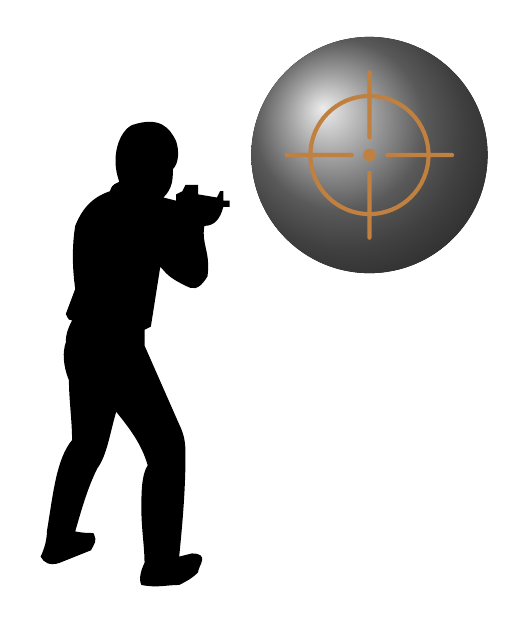
\begin{tikzpicture}[line cap=round,line join=round,scale=1]
				\def\muctieu{\tikz{ 
				\fill[ball color=gray] (0,0)  circle (2cm);
				\fill[brown] circle (3pt); 
				 \draw[teal,line width=2pt,brown] circle (1cm)
					 (90:0.3)--++(0,1.1)
					(-90:0.3)--++(0,-1.1) 
					(0:0.3)--++(1.1,0) 
					 (180:0.3)--++(-1.1,0);
					 }}
				\def\nguoi{ 
				\tikz[yscale=-1]{ 
				\fill  (3.1,16.8).. controls (2.8,16.0) and
					(3.1,15.2).. (3.5,15.0)..  controls (4.4,14.7) and (4.7,15.1).. (4.9,
					15.5).. controls (5.0,15.8) and (5.0,16.2)..  (4.8,16.4).. controls (4.8,
					16.7) and (4.8,17.0).. (4.5,17.3) -- (4.9,17.4)  -- (4.9,17.2) -- (5.1,
					 17.1) -- (5.2,16.9) -- (5.6,16.9) -- (5.6,17.2) -- (6.2,17.3) -- (6.3,
					17.1) -- (6.4,17.1) -- (6.4,17.4) --  (6.6,17.4) -- (6.6,17.6) -- (6.4,
					17.6).. controls (6.3,18.0) and  (6.1,18.2).. (5.8,18.2).. controls (5.7,
					18.8) and  (6.0,19.0).. (5.9,19.8).. controls (5.6,20.3) and (5.4,20.2)..
					(5.2,20.1).. controls (4.6,19.8) and (4.6,19.7).. (4.4,19.5) -- (4.1, 
					21.4) -- (3.9,21.5) -- (3.9,22.0) -- (5.0,24.5)..  controls (5.2,24.9) and
					(5.2,25.2).. (5.2,25.5).. controls (5.2,26.6) and  (5.1,27.7).. (5.0,
					28.7) -- (5.4,28.6).. controls (6.0,28.6) and  (5.6,29.0).. (5.6,29.2)..
					 controls (5.4,29.4) and (5.2,29.5).. (5.0,29.6).. controls (4.6,29.6) and
					(4.3,29.7)..  (3.8,29.6).. controls (3.7,29.4) and (3.8,29.1).. (3.9,
					28.9).. controls  (3.9,28.4) and (3.8,27.8).. (3.8,27.2).. controls (3.8,
					26.7) and (3.8,26.1).. (4.0,25.8).. controls (3.8,25.1)  and (3.4,24.6)..
					(3.0,24.1).. controls (2.8,24.8)  and (2.7,25.5).. (2.4,25.9).. controls
					(2.1,26.5) and (1.9,27.2).. (1.7,27.9).. controls (2.2,28.0) and (2.3, 
					27.9).. (2.3,28.0).. controls (2.4,28.2) and (2.3,28.3).. (2.2,28.5) -- 
					(1.2,28.9).. controls (0.9,29.0) and (0.7,28.9)..  (0.6,28.7).. controls
					(0.7,28.5) and  (0.8,28.2).. (0.8,27.9).. controls (1.0,26.7) and (1.1,
					25.6).. (1.6,25.0).. controls (1.6,24.4) and (1.5,23.7).. (1.5,23.1).. 
					controls (1.3,22.6) and (1.3,22.2).. (1.4,21.9).. controls (1.4,21.6)  and
					(1.5,21.4).. (1.6,21.2).. controls  (1.5,21.2) and (1.5,21.2).. (1.4,
					21.0) -- (1.7,20.2).. controls (1.6,19.5) and (1.6,18.8).. (1.7,18.2).. 
					controls (1.9,17.7) and (2.2,17.3).. (2.8,17.1).. controls  (2.9,16.8) and
					 (3.0,16.9).. (3.1,16.8) -- cycle;
					 }}
				\path (3,2.5) coordinate (B) 
					(0,0) coordinate (A); 
				\path (A)  node (nA) {\resizebox{!}{6cm}{\nguoi}};
				\path  (B) node (nB) {\resizebox{!}{3cm}{\muctieu}};
			\end{tikzpicture}
	\end{center}
	 \choiceTF
		{\True  Mặt cầu $(S)$ có tâm $I(-1;2;1)$ và bán kính $R=1$}
		 {\True Mặt phẳng $(P)$ và mặt cầu $(S)$ không có điểm chung}
		{\True Người chơi đứng ở  vị trí giao của mặt phẳng $(P)$ với trục $Ox$, khoảng cách từ tâm của quả cầu đến đường bay của viên đạn bằng $\dfrac{\sqrt{66}}{2}$}
		{\True Khoảng cách lớn nhất từ vị trí người bắn đến mục tiêu bằng $3\sqrt{2}$} 
	\loigiai{ 
		\begin{itemchoice}
			\itemch Mặt cầu $(S)$ có tâm $I(-1; 2; 1)$ và  bán kính $R = 1$.
			\itemch Ta có $\mathrm{d}(I, (P))=\frac{|-1-4+2-3|}{\sqrt{1+4+4}} = 2 >  R$; do đó $(P)$ và mặt cầu $(S)$ không có điểm chung.
			\itemch Giao điểm của $(P)$ và $Ox$ là điểm $M_0(3; 0; 0)  \Rightarrow \vec{IM} = (4; -2; -1) \Rightarrow \left[\vec{IM}, \vec{u}\right] = (-2; -5; 2)$.\\
			Khoảng cách từ $I$ đến đường  bay viên đạn là
			\[\mathrm{d} = \dfrac{\left|[\vec{IM}, \vec{u}]\right|}{\left|\vec{u}\right|} = \dfrac{\sqrt{4+25+4}}{\sqrt{1+0+1}} = \dfrac{\sqrt{66}}{2}.\] 
			\itemch Gọi $M$ thuộc $(P)$, $N$ thuộc $(S)$ theo thứ tự là vị trí người chơi và vị trí mục tiêu đang bắn; $H$  là hình chiếu của điểm $N$ trên $(P)$. $MN$ hợp với $(P)$ một góc $\varphi$ thỏa mãn
			 \[\sin \varphi = \dfrac{\left|\vec{u} \cdot \vec{n}_P\right|}{\left|\vec{u}\right| \cdot \left|\vec{n}_P\right|} = \dfrac{|1+0+2|}{\sqrt{1+0+1} \cdot \sqrt{1+4+4}} = \dfrac{\sqrt{2}}{2}.\]
		 \immini{
			Xét  tam giác $MNH$ vuông tại $H$, ta có
			$$\sin \varphi = \dfrac{NH}{MN} \Rightarrow MN  = \dfrac{NH}{\sin \varphi } \text{ hay } MN = \sqrt{2}NH.$$
			Dễ thấy $MN$ lớn nhất  khi và chỉ khi $NH$ lớn nhất.\\
			Mà $NH \le \mathrm{d}(I, (P)) + R  = 2+1=3.$\\
			Do đó $MN$ lớn nhất bằng $3\sqrt{2}$ khi đó $N$, $I$,  $H$ thẳng hàng.
			 }{
			\begin{tikzpicture}[line join=round,line cap=round,scale=1]
					\path 
						(0,0) coordinate  (I)
						(0,1.5) coordinate  (N)
						(0,-3) coordinate  (H)
						(2,-3) coordinate  (M)
						 (-2,-2) coordinate (P1)
						 (-3,-4) coordinate (P2)
						 (2,-4) coordinate (P3)
						($(P1)+(P3)-(P2)$)  coordinate (P4)
						 (intersection of M--N and P1--P4) coordinate (P41)
						(intersection  of H--N and P1--P4) coordinate (P11);
					\path[name path=c]  (I) circle (1.5);
					\path[name path=l1] (M)--(N); 
					\path[name path=l2] (H)--(N); 
					\path[name intersections={of=c and l1}]  (intersection-2) coordinate (M1);
					\path[name intersections={of=c and l2}] (intersection-2)  coordinate (H1);
					\draw[teal]  (I) circle (1.5)
						 (1.5,0) node[right]{$(S)$}
						 (P11)--(P1)--(P2)--(P3)--(P4)--(P41)
						 (M1)--(M)--(H)--(H1);
					\draw[teal,dashed,thin]  (P11)--(P41)
						 (M1)--(N)--(H1);
					 \pic[draw,thin,angle radius=2mm] {right angle = N--H--M};
					\draw[teal] pic["{\scriptsize $\varphi$}",draw,angle  eccentricity=1.5,angle radius=0.4cm]{angle=N--M--H};
					\draw[teal]  pic["{\scriptsize $P$}",draw,angle eccentricity=0.65,angle radius=0.7cm]{angle=P3--P2--P1};
					\foreach  \i/\g in {I/180,N/90,H/-110,M/-60}{\fill (\i) circle (1.5pt)
						($(\i)+(\g:3mm)$)  node[scale=1]{$\i$};}
				\end{tikzpicture}
			} 
		\end{itemchoice}
	 }
\end{ex}

% nguồn: Phan1_Lop_12_Hinh_hoc_Chuong_5
\begin{ex}%[2H5V3-4]%[ma:7f098e9f]
	Một tàu cứu hộ đang ở vị trí $A(1;-2; 2)$ (đơn vị km) và di chuyển theo đường thẳng với vectơ vận tốc $\vec{v}=(-2; 4; 1)$ (km/giờ). Một cơn bão đang hình thành biết vùng nguy hiểm được  mô tả bởi một hình cầu có tâm bão tại $B(-3; 0; 4)$ (đơn vị km) và bán kính $R=6$ km.
	 \choiceTF
		{Phương trình mô tả ranh giới vùng nguy hiểm  của cơn bão là $(x+3)^2+y^2+(z-4)^2=6$}
		{\True Phương trình tham số của đường thẳng biểu diễn quỹ đạo di chuyển của tàu cứu hộ là $\heva{&x=1-2t \\ &y=-2+4t\\  &z=2+t}, t \geq 0$}
		 {\True Khoảng thời gian mà tàu ở trong vùng nguy hiểm là $2$ giờ}
		{\True Khoảng  cách ngắn nhất từ tàu cứu hộ đến tâm bão là $3$ km (kết quả làm tròn đến hàng đơn vị của km)}
	\loigiai{ 
		\begin{itemchoice}
			\itemch Phương trình mô tả ranh giới vùng nguy hiểm của cơn bão là  phương trình mặt cầu tâm $B(-3;0;4)$ bán kính $R=6$: $(x+3)^2+y^2+(z-4)^2=36$.
			\itemch Phương trình đường  thẳng biểu diễn quỹ đạo tàu đi qua $A(1;-2;2)$ và có vectơ chỉ phương $\vec{v}=(-2; 4; 1)$ là $\heva{&x=1-2t \\ &y=-2+4t\\ &z=2+t}, t \geq 0$.
			\itemch Gọi $M(1-2t;-2+4t;2+t)$ là một điểm bất kỳ nằm trên  quỹ đạo của tàu cứu hộ.\\
			Khi đó tàu ở trong  vùng nguy hiểm khi
			\begin{eqnarray*}
				BM\leq 6&\Leftrightarrow& BM^2\leq 36\\ 
				&\Leftrightarrow&  (4-2t)^2+(4t-2)^2+(2-t)^2\leq 36\\
				 &\Leftrightarrow& 21t^2-36t-12\leq0\\
				&\Leftrightarrow& -\dfrac{2}{7}\leq  t\leq 2.
			\end{eqnarray*}
			Do $t\geq0$ nên ta có $0\leq t\leq  2$ suy ra khoảng thời gian tàu ở trong vùng nguy hiểm là $2-0=2$ giờ.
			\itemch Khoảng cách ngắn nhất của tàu đến tâm bão là  $BM_{\min}\Leftrightarrow BM^2_{\min}$.\\
			Ta có $BM^2=(4-2t)^2+(4t-2)^2+(2-t)^2=21t^2-36t+24$  đạt giá trị nhỏ nhất tại $t=\dfrac{36}{42}$.\\
			 Khi đó $BM=\sqrt{\left(4-\dfrac{2\cdot36}{42}\right)^2+\left(\dfrac{4\cdot36}{42}-2\right)^2+\left(2-\dfrac{36}{42}\right)^2}\approx3$ km.
		\end{itemchoice}
	} 
\end{ex}

% nguồn: Phan1_Lop_12_Hinh_hoc_Chuong_5
\begin{ex}%[2H5V3-4]%[ma:c6b77749]
	\immini[thm]{Sao Thủy gần như không có khí quyển thật sự như Trái Đất hay Sao Kim. Tuy nhiên, nó có một lớp khí rất mỏng gọi là exosphere - tức là thượng quyển loãng, gồm các hạt khí cực kỳ thưa thớt như hydro, heli, oxy, natri,...Trong không gian $Oxyz$, đơn vị trên mỗi trục là nghìn km, vùng thượng quyển loãng của  Sao Thủy được mô hình hóa bởi phương trình mặt cầu \break $x^2+y^2+z^2-2x-4y-4=0$.}
	{\begin{tikzpicture}[scale=0.8,font=\footnotesize,line join=round,line cap=round,>=stealth]
		\def\cau#1#2#3{ 
		 \def\r{#1}
		\shade[ball color=#2,opacity=1,shading angle=-110]  #3 circle (\r);
		\begin{scope}
			\clip #3 circle (\r); 
			\foreach \i in  {1,...,300}{
				 \pgfmathsetmacro{\x}{(rand*2-1)*\r}
				 \pgfmathsetmacro{\y}{(rand*2-1)*\r}
				 \pgfmathsetmacro{\s}{0.02*\r + 0.03*\r*rand}
				\fill[white,opacity=.08] #3 ++(\x,\y) circle (\s); 
			} 
			\foreach \i in {1,...,200}{ 
				\pgfmathsetmacro{\x}{(rand*2-1)*\r} 
				 \pgfmathsetmacro{\y}{(rand*2-1)*\r}
				\pgfmathsetmacro{\s}{0.02*\r  + 0.03*\r*rand}
				\fill[opacity=.06] #3 ++(\x,\y) circle (\s); 
			} 
		\end{scope}
		 }
		\fill[gray!50] (-5,-3) rectangle (5,3); 
		 \cau{2.8}{brown!85!yellow}{(0,0)}
		 \cau{0.5}{gray!50}{(4,0)} \path (4,-0.5) node[below,scale=1.5]{$B$};
		\cau{0.5}{gray}{(-4,0)} \path  (-4,-0.5) node[below,scale=1.5]{$A$};
		\fill[white] (-4.75,1)  circle (4pt);
		\draw[white,path fading = north,line width=3pt]  (-4.75,1)--++(25:2.75cm);
	\end{tikzpicture}
	 }
	\noindent 
	Các nhà khoa học không gian đang quan sát các tiểu hành tinh ở các vị trí có tọa độ $A(4;2;4)$, $B(1;4;2)$ và xem xét sự di chuyển  của chúng. Nếu tiểu hành tinh nằm trong vùng thượng quyển loãng thì nó sẽ bị hút xuống bề mặt Sao Thủy.
	 \choiceTF
		{\True  Vùng thượng quyển loãng Sao Thủy có tâm $(1;2;0)$, bán kính bằng $3$}
		{Hai tiểu hành tinh ở các vị trí $A$, $B$ sẽ bị hút xuống bề mặt Sao Thủy} 
		{Các nhà quan sát cho rằng có một sao chổi mang tên Haxen di chuyển theo quỹ đạo đường thẳng với vận tốc $51{,}5$ km/s khoảng cách ngắn nhất từ tâm Sao Thủy đến Sao Chổi bằng $\dfrac{\sqrt{871}}{10}$ nghìn km. Thời gian Sao Chổi đi trong vùng  thượng quyển loãng của Sao Thủy bằng $20$ giây (làm tròn đến hàng đơn vị của giây)}
		{\True Sao Chổi Haxen di chuyển theo phương vectơ $\vv{u}=(0;5;2)$. Giả sử $M$, $N$  là điểm đầu và điểm cuối mà sao chổi này đi qua thuộc vùng thượng quyển loãng của Sao Thủy. Giá trị nhỏ nhất của tổng $AM+B N$ bằng $3\,970$ km (làm tròn đến hàng đơn vị của km)}
	 \loigiai{
		\begin{itemchoice}
			\itemch Vùng thượng quyển loãng Sao  Thủy có tâm $I(1;2;0)$, bán kính $R=\sqrt{1^2+2^2+0^2+4}=3$.
			\itemch Ta có $IA=\sqrt{(4-1)^2+(2-2)^2+(4-0)^2}=5$, $IB=\sqrt{(1-1)^2+(4-2)^2+(2-0)^2}=2  \sqrt{2}$.\\
			Vì $IA>R$, $IB<R$ nên tiểu hành tinh $A$ nằm ngoài vùng thượng quyển loãng, còn tiểu hành tinh $B$  thì nằm tròn vùng thượng quyển loãng của Sao Thủy và nó sẽ bị hút xuống bề mặt Sao Thủy.
			\itemch Gọi $d$ là quỹ đạo đường thẳng của Sao Chổi và $H$ là hình chiếu vuông góc của tâm $I$ trên $d$.\\ 
			Gọi $M$, $N$ là điểm đầu và điểm cuối của Sao Chổi trong vùng thượng quyển  loãng của Sao Thủy.\\
			Ta có $IH=\dfrac{\sqrt{871}}{10}$.\\ 
			Suy ra $MN=2MH=2 \sqrt{R^2-I H^2}=2 \sqrt{9-\frac{871}{100}}=\dfrac{\sqrt{29}}{5}$ (nghìn  km).\\
			Thời gian Sao  Chổi di chuyển trong vùng thượng quyển loãng $\dfrac{\sqrt{29}}{5} \cdot \dfrac{1\,000}{51{,}5} \approx 21$ (giây).
			 \itemch
			\begin{center}
				\begin{tikzpicture}[line join=round,line cap=round,>=stealth]
						\coordinate (I) at  (0,0);
						\coordinate (M) at ($(I) + (230:2.5)$); 
						 \coordinate (N) at ($(I) + (310:2.5)$);
						\coordinate (H) at  ($(M)!0.5!(N)$);
						\coordinate (b) at ($(I)  + (300:2.5)$);
						 \coordinate (A) at (-1,-3);
						\coordinate  (C) at ($(A) + (b)-(M)$);
						\coordinate (B)  at ($(C)!1.5!(b)$);
						\draw[name path=(I)] (I) circle (2.5 cm); 
						\draw  (I)--(M)--(N)
						(B)--(b) 
						 (I)--(H);
						\draw  [->] (M)--(b);
						 \draw[dashed] (A)--(C);
						\draw [dashed] (C)--(b) 
						(M)--(A); 
						\draw pic[draw,angle  radius=0.3cm]{right angle=I--H--N};
						\foreach \i/\g in {I/90,M/-140,N/-45,H/130,A/-120,C/-45,B/90}{\draw (\i) circle (1.2pt) 
						 ($(\i)+(\g:3mm)$) node[scale=1]{$\i$};}
					\end{tikzpicture}
			\end{center}
			Đặt $\overrightarrow{MN}=(0;5 k;2 k)$, ta có  $MN^2=25 k^2+4 k^2=\dfrac{29}{25} \Rightarrow k=\dfrac{1}{5}$.\\
			 Suy ra $\overrightarrow{MN}=\left(0;1;\dfrac{2}{5}\right)$.\\
			Chọn  $C$ sao cho $AMNC$ là hình bình hành.\\
			Suy ra  $C\left(4;3;\dfrac{22}{5}\right)$.\\
			Khi đó $AM=CN$ và $AM+BN=CN+BN \geq BC=\dfrac{\sqrt{394}}{5} \approx  3{,}97$.\\
			Vậy giá trị  nhỏ nhất của biểu thức $AM+BN$ là khoảng $3\,970$ km.
		\end{itemchoice}
	 }
\end{ex}

% nguồn: Phan1_Lop_12_Hinh_hoc_Chuong_5
\begin{ex}%[2H5V3-4]%[ma:b0c12f23]
	Một tiểu hành tinh nhỏ (coi như một hạt) được phát hiện đang bay theo chuyển động thẳng đều trong không gian $Oxyz$ với $O$ là tâm Trái Đất. Tại thời điểm $t=0$, tiểu hành tinh ở vị trí $A(10\,000;5\,000;8\,000)$ (km), bay theo hướng vectơ $\overrightarrow{v}=(-300;-100;-160)$ (km/h). Coi  bề mặt Trái Đất là mặt cầu bán kính $6\,371$ (km).
	\choiceTF 
		 {\True Phương trình mặt cầu biểu diễn bề mặt Trái Đất là $x^2+y^2+z^2=40\,589\,641$}
		{\True Phương trình đường thẳng mô tả quỹ đạo của tiểu hành tinh là $\heva{&x=10\,000-300t\\&y=5\,000-100t\\&z=8\,000-160t}$, $t\ge 0$} 
		{\True Tại thời điểm $5$ giờ kể từ khi phát hiện, tiểu hành tinh ở vị trí  có tọa độ $(8\,500;4\,500;7\,200)$ (km)}
		{\True Thời điểm tiểu hành tinh va chạm  với Trái Đất là sau $21$ giờ $43$ phút (làm tròn đến đơn vị phút)}
	\loigiai{ 
		\begin{itemchoice}
			 \itemch Phương trình mặt cầu biểu diễn bề mặt Trái Đất là
			\[x^2+y^2+z^2=6\,371^2 \Leftrightarrow  x^2+y^2+z^2=40\,589\,641.\]
			\itemch Tại thời điểm $t=0$, tiểu hành tinh ở vị trí $A(10\,000;5\,000;8\,000)$ (km), bay theo hướng vectơ $\overrightarrow{v}=(-300;-100;-160)$ (km/h) nên vị trí của tiểu hành tinh tại thời điểm $t$ là $\heva{&x=10\,000-300t\\&y=5\,000-100t\\&z=8\,000-160t}$ với $t  \ge 0$.
			\itemch Tại thời điểm $5$  giờ kể từ khi phát hiện, tiểu hành tinh ở vị trí có tọa độ
			\[\heva{&x=10\,000-300 \cdot 5\\&y=5\,000-100 \cdot  5\\&z=8\,000-160 \cdot 5} \Leftrightarrow \heva{&x=8\,500\\&y=4\,500\\&z=7\,200.}\]
			\itemch Gọi $B$ là điểm va  chạm của tiểu hành tinh với Trái Đất.\\
			Vì điểm $B$  thuộc đường thẳng mô tả quỹ đạo của tiểu hành tinh nên $B(10\,000-300t;5\,000-100t;8\,000-160t)$.\\
			Vì $B$ thuộc vào mặt cầu biểu diễn bề mặt  Trái Đất nên ta có
			\[(10\,000-300t)^2+(5\,000-100t)^2+(8\,000-160t)^2=40\,589\,641 \Leftrightarrow \hoac{&t \approx 21{,}72\\&t \approx 54{,}39.}\] 
			Vậy thời điểm va chạm đầu tiên của hành tinh là tại $t=21{,}72$  h hay $21$ giờ $43$ phút.
	\end{itemchoice}}
\end{ex}

% nguồn: Phan1_Lop_12_Hinh_hoc_Chuong_5
\begin{ex}%[2H5V3-4]%[ma:227d1c13]
	Ngày nay, nhờ vào hệ thống định vị toàn cầu GPS (Global Positioning System), việc di chuyển của con người hết sức thuận lợi dù bằng đường bộ, đường sắt hay đường hàng không hay đường biển. Nếu có thiết bị bắt sóng GPS, bạn luôn có thể kết nối được đến bốn vệ tinh GPS dù ở bất kì đâu trên Trái Đất. Khi thiết bị của bạn biết khoảng từ ít nhất ba vệ tinh đến nó, máy sẽ tính toán ra vị trí hiện tại của bạn bằng một quy trình gọi là Trolateration. Cho biết trái đất có dạng hình cầu bán kính bằng $\sqrt{41}\cdot10^{3}$ km. Bạn An đang đứng trên mặt đất. Có ba vệ tinh báo về máy chủ tiếp nhận  thông tin rằng vệ tinh thứ nhất đang cách An $3\cdot10^{3}$ km, vệ tinh thứ hai đang cách An $5\cdot10^{3}$ km, vệ tinh thứ ba đang cách An $4\cdot10^{3}$ km. Chọn hệ trục tọa độ $Oxyz$ với $O$ là tâm trái đất và đơn vị độ dài trên mỗi trục là $10^3$ km. Tại thời điểm vệ tinh thông báo về máy chủ thì tọa độ của các vệ tinh lần lượt là $I_1\left(4;4;6\right)$, $I_2\left(4;9;3\right)$ và $I_3\left(8;4;3\right)$. Xem vị trí An là điểm $A$ và An cần di chuyển thẳng đến nhà Bình là điểm $B\left(4;4;3{,}01\right)$ với tốc độ không đổi $20$ km/h.
	 \choiceTF
		{\True Điểm $A$ đang nằm trên mặt  cầu tâm $O$ bán kính $\sqrt{41}\cdot10^3$ km}
		{Phương  trình mặt cầu mô tả ranh giới bên trong và bên ngoài Trái Đất là
		$x^2+y^2+z^2=\sqrt{41}$} 
		{\True Điểm $A$ chính là giao điểm của bốn mặt cầu: Trái Đất và ba mặt cầu tâm lần lượt là  $I_1$, $I_2$, $I_3$ có bán kính lần lượt là khoảng cách từ các vệ tinh đến An}
		{Thời gian An đi đến nhà Bình là $30$  phút}
	 \loigiai{
		\begin{itemchoice}
			 \itemch
			Điểm $A$ nằm  trên mặt đất nên nằm trên mặt cầu tâm $O$ bán kính $\sqrt{41}\cdot10^{3}$ km.
			\itemch 
			Phương trình mặt cầu mô  tả ranh giới bên trong và bên ngoài Trái Đất có tâm $O(0;0;0)$, bán kính $R=\sqrt{41}$ là $x^{2}+y^{2}+z^{2}=41$.
			\itemch 
			Điểm $A$ chính là giao điểm của bốn mặt cầu: Trái Đất và ba mặt cầu tâm lần lượt là $I_1$, $I_2$, $I_3$ có bán kính lần lượt là khoảng cách  từ các vệ tinh đến An.
			\begin{itemize}
				\item Mặt cầu Trái  Đất $x^2+y^2+z^2=41$.
				\item Mặt cầu tâm $I_1$, bán kính $R=3$ có phương trình  $\left(x-4\right)^{2}+\left(y-4\right)^{2}+\left(z-6\right)^{2}=9$.
				\item Mặt cầu tâm $I_2$, bán kính $R=5$ có phương trình $\left(x-4\right)^{2}+\left(y-9\right)^{2}+\left(z-3\right)^{2}=25$. 
				\item Mặt  cầu tâm $I_3$, bán kính $R=4$ có phương trình $\left(x-8\right)^{2}+\left(y-4\right)^{2}+\left(z-3\right)^{2}=16$.
			\end{itemize}
			Xét hệ 
			$\heva{&x^{2}+y^{2}+z^{2}=41\\ &\left(x-4\right)^{2}+\left(y-4\right) ^{2}+\left(z-6\right)^{2}=9 \\ &\left(x-4\right)^{2}+\left(y-9\right)^{2}+\left(z-3\right)^{2}=25 \\ &\left(x-8\right)^{2}+\left(y-4\right)^{2}+\left(z-3\right)^{2}=16}\Rightarrow  \heva{&x=4 \\&y=4 \\&z=3.}$\\
			Vậy  $A\left(4;4;3\right)$.
			\itemch 
			Khoảng cách giữa An với Bình là 
			$AB=\sqrt{\left(4-4\right)^{2}+\left(4-4\right)^{2}+\left(3{,}01-3\right)^{2}}=0{,}01$.\\ 
			Thời gian An đi đến  nhà Bình là
			$t=\dfrac{AB}{v}=\dfrac{0{,}01\cdot10^{3}}{20}\cdot60=30$  (phút).
		\end{itemchoice}
	 }
	\loigiai{} 
\end{ex}

% nguồn: Phan1_Lop_12_Hinh_hoc_Chuong_5
\begin{ex}%[2H5V3-4]%[ma:7c3a7478]
	Các thiên thạch có đường kính lớn hơn $140$ m và có thể lại gần Trái Đất  ở khoảng cách nhỏ hơn $7\,500\,000$ km được coi là những vật thể có khả năng va chạm gây nguy hiểm cho Trái Đất. Để theo dõi những thiên thạch này, người ta đã thiết lập các trạm quan sát các vật thể bay gần Trái Đất. Giả sử có một hệ thống quan sát có khả năng theo dõi các vật thể ở độ cao không vượt quá 6 600 km so với mực nước biển. Coi Trái Đất là khối cầu có bán kính $6\,400$ km. Chọn hệ trục tọa độ $Oxyz$ trong không gian có gốc $O$ tại tâm Trái Đất và đơn vị độ dài trên mỗi trục tọa độ là $1\,000$ km. Một thiên thạch (coi như một hạt) chuyển động với tốc độ không đổi theo một đường thẳng từ điểm $M(6;20;0)$ đến điểm $N(-6;-12;16)$.
	\begin{center}
		\begin{tikzpicture}[scale=1,font=\footnotesize,line join=round,line cap=round,>=stealth]
				 \def \r{1.5}
				\path 
					(0,0) coordinate  (O)
					(130:2*\r) coordinate  (A)
					 (40:2*\r) coordinate (B)
					($(A)!1.3!(B)$) coordinate  (N)
					($(B)!1.2!(A)$) coordinate (M) 
					(0:\r) coordinate (X) 
					(0:2*\r)  coordinate (Y)
					($(O)!0.5!(X)$) coordinate  (x) node[above]{$6\,400\,\mathrm{km}$}
					 ($(X)!0.5!(Y)$) coordinate (x) node[above]{$6\,600\,\mathrm{km}$};
				 \draw (O) circle (\r);
				\draw (O)  circle (2*\r);
				 \draw (M)--(N);
				\draw[<->] (O)--(X); 
				\draw[<->] (X)--(Y); 
				\foreach \x/\g  in {A/100,B/80,M/120,N/40,O/-90}\fill (\x) circle (1pt)+(\g:.3) node{$\x$};
			\end{tikzpicture}
	\end{center}
	\choiceTF 
		{\True Đường thẳng $MN$ có phương trình tham  số là $\heva{& x=6+3t\\&y=20+8t\\& z=-4t}$ ($t\in \mathbb{R}$)}
		{Vị trí đầu tiên thiên thạch di  chuyển vào phạm vi theo dõi của hệ thống quan sát là điểm $A(-3;-4;12)$}
		{\True Khoảng cách giữa vị trí đầu tiên và vị trí cuối cùng mà thiên thạch di chuyển trong phạm vi theo dõi của hệ thống quan sát là $18\,900$ km (kết quả làm  tròn đến hàng trăm theo đơn vị km)}
		{\True Nếu thời gian di  chuyển của thiên thạch trong phạm vi theo dõi của hệ thống quan sát là $3$ phút thì thời gian nó di chuyển từ $M$ đến $N$ là $6$ phút}
	 \loigiai{
		\begin{itemchoice}
			\itemch Vectơ chỉ phương của đường thẳng $MN$  là $\overrightarrow{MN}=(-12;-32;16)=-4(3;8;-4)$.\\
			Phương  trình tham số của đường thẳng $MN$ là $\heva{& x=6+3t\\&y=20+8t\\& z=-4t}$, $t\in \mathbb{R}$.\\
			\itemch Để tìm vị trí đầu tiên thiên thạch di chuyển vào phạm vi theo dõi, ta cần tìm điểm giao  của đường thẳng $MN$ với mặt cầu có tâm $O(0;0;0)$ và bán kính $R~=6{,}4+6{,}6=13$.\\
			Phương trình mặt cầu là $x^2+y^2+z^2=13^2$.\\ 
			Thay $x=6~+~3t$; $y=20~+~8t$ và $z=-4t$ vào phương trình mặt cầu ta  được
			 \allowdisplaybreaks
			\begin{eqnarray*}
				&&(6+3t)^2+(20+8t)^2+(-4t)^2=13^2\\ 
				 &\Leftrightarrow& 89t^2+356t+267=0\\
				&\Leftrightarrow&  \hoac{&t=-3\\&t=-1.}
			\end{eqnarray*}
			Với $t=-3$  ta được tọa độ $(3;12;4)$.\\
			Với $t=-1$ ta được tọa độ  $(-3;-4;12)$.\\
			Nhận thấy từ $M$ đến  $N$ thì hoành độ có xu hương giảm dần nên điểm $A(3;12;4)$.
			\itemch Ta  có $B(-3;-4;12)$.\\
			Khoảng cách giữa vị trí đầu tiên và vị trí cuối cùng $AB$  là\\
			$AB=\sqrt{(-3-3)^2+(-4-12)^2+(12-4)^2}=2\sqrt{89}$ tương đương với $\approx 18\,900$  km.
			\itemch  Thời gian thiên thạch di chuyển từ $M$ đến $N$ là\\
			$MN=\sqrt{(6+6)^2+(-12-20)^2+(16-0)^2}=4\sqrt{89}=2AB$ nên do đó $t=\dfrac{MN}{AB}\cdot3\approx 6$  phút.
		\end{itemchoice}
	 }
\end{ex}

% nguồn: Phan1_Lop_12_Hinh_hoc_Chuong_5
\begin{ex}%[2H5V3-4]%[ma:80dda0a4]
	Trong không gian hệ trục tọa độ $Oxyz$ (đơn vị trên mỗi trục  là kilômét), đài kiểm soát không lưu của một sân bay ở vị trí $O(0;0;0)$ và được thiết kế phát hiện máy bay ở khoảng cách tối đa $600$ km. Một máy bay đang chuyển động với vận tốc $900 \mathrm{~km}/\mathrm{h}$ theo đường thẳng $d$ có phương trình $\heva{&x=-1\,000+100t\\&y=-300+80t\\&z=100\sqrt{11}}$, $t\in \mathbb{R}$ và hướng về đài kiểm soát không lưu (như hình vẽ).
	\begin{center}
		\begin{tikzpicture}[>=stealth,line join=round,line cap=round,font=\footnotesize,scale=1]
				\tikzset{declare function={r=2; r2=.8;}} 
				\path 
					(0,0)  coordinate (O)+
					(0:r)  coordinate (M)+
					(180:r) coordinate (N)+(90:1.4*r) coordinate (z) 
					(90:.8*r) coordinate  (z1)
					(-90:1.5*r) coordinate  (z2)
					(0:r*1.4)  coordinate (y)
					 (180:r*1.4) coordinate (y')
					(-130:r*1.4) coordinate  (x)
					(165:r*1.5) coordinate (A) 
					 (2:r*1.5) coordinate (d)
					($(x)!.6!(O)$)  coordinate (x1)
					($(x)!2!(O)$) coordinate (x2) 
					($(A)!.25!(d)$)  coordinate (B)
					($(A)!.7!(d)$) coordinate  (C);
				\draw (0,0) circle (r); 
				 \draw (N) arc (180:360:r and r2);
				\draw[dashed](N) arc  (180:0:r and r2);
				\foreach \pointo/\pointt in  {M/N,z1/z2,x1/x2,B/C}{
					\draw[dashed](\pointo)--(\pointt); 
				} 
				\foreach \pointo/\pointt  in {N/y',A/B,C/d}{
					\draw (\pointo)--(\pointt); 
				 }
				\foreach \pointo/\pointt in  {z1/z,M/y,x1/x}{
					\draw[->](\pointo)--(\pointt); 
				 }
				\foreach \point/\goc in  {A/90,B/90,C/90,z/180,x/170,y/-90}{
					\draw (\point) circle (0pt)+(\goc:2mm)  node[scale=.8]{$\point$};
				 }
				\foreach \point/\goc in  {O/-45}{
					\draw  (\point) circle (.8pt)+(\goc:2mm) node[scale=.8]{$\point$};
				 }
			\end{tikzpicture}
	\end{center}
	\choiceTF 
		{\True Phương trình mặt cầu để mô tả ranh giới bên ngoài vùng phát sóng của  đài kiểm soát không lưu trong không gian là $x^2+y^2+z^2=360\,000$}
		{\True Máy bay đang chuyển động theo đường thẳng $d$ đến vị  trí điểm $M(-500; 100; 100 \sqrt{11})$. Vị trí này nằm ngoài vùng kiểm soát không lưu của đài kiểm soát không lưu sân bay}
		{Thời gian kể từ khi đài kiểm soát không lưu phát hiện may bay đến  khi máy ra khỏi vùng kiểm soát không lưu là $\dfrac{4}{3}$ giờ}
		{Ranh giới vùng  phát sóng bên ngoài của đài kiểm soát không lưu trong không gian là mặt cầu có bán kính bằng $300$ km}
	 \loigiai{
		\begin{itemchoice}
			\itemch Mặt cầu để mô tả ranh giới bên ngoài vùng phát sóng của đài kiểm soát không lưu trong không gian có tâm $O(0;0;0)$ và bán kính $R=600$ có phương  trình là
			\[(S)\colon x^2+y^2+z^2=600^2=360\,000\] 
			\itemch $OM=\sqrt{(-500)^2+100^2+\left(100\sqrt{11}\right)^2}\approx 608>R$.\\ 
			Suy ra vị  trí $M$ nằm ngoài vùng kiểm soát không lưu của đài kiểm soát không lưu sân bay.
			\itemch  Gọi $B=(S)\cap d$, $C=(S)\cap d$.\\
			Ta có  $B\in d\Rightarrow B(-1\,000+100t;-300+80t;100\sqrt{11})$.\\
			Mặt khác  $B\in (S)$ nên
			\begin{eqnarray*}
				(-1\,000+100t)^2+(-300+80t)^2+(100\sqrt{11})^2&=&360\,000\\ 
				 16\,400t^2-248\,000t+840\,000&=&0\\
				t=10 \ \text{  hoặc} \ t&=&\dfrac{210}{41}.
			\end{eqnarray*}
			Do đó $B(0;500;100\sqrt{11})$ và  $C\left(-\dfrac{20\,000}{41};\dfrac{4\,500}{41};100\sqrt{11}\right)$.\\
			Ta có $BC\approx  624{,}7$.\\
			Thời gian kể  từ khi đài kiểm soát không lưu phát hiện may bay đến khi máy ra khỏi vùng kiểm soát không lưu là
			\[\dfrac{BC}{900}\approx 0{,}69\ \text{  (giờ)}.\]
			\itemch 
			Ranh giới  vùng phát sóng bên ngoài của đài kiểm soát không lưu trong không gian là mặt cầu có bán kính bằng $300$ km.
		\end{itemchoice}
	 }
\end{ex}

% nguồn: Phan1_Lop_12_Hinh_hoc_Chuong_5
\begin{ex}%[2H5V3-4]%[ma:eed2c453]
	Trong  không gian $Oxyz$ cho trước, đơn~vị trên mỗi trục là mét, có hai chiếc chiến đấu cơ từ hai vị trí $A(40;-15; 15), B(55;-10; 65)$ cần đáp xuống hai vị trí thuộc tàu sân bay hải quân để nạp nhiên liệu. Bề mặt chứa các đường băng trên tàu là mặt phẳng $(P)$ có phương trình $3x-y+2z-25=0$.
	Xét tính đúng sai các mệnh đề sau 
	\choiceTF 
		{Đường thẳng qua $A$  và vuông góc với mặt phẳng $(P)$ có phương trình chính tắc là $\dfrac{x-40}{3}=\dfrac{y+15}{1}=\dfrac{z-15}{-2}$}
		{Tổng khoảng cách từ hai vị trí chiến đấu cơ đến mặt phẳng chứa đường  băng là $110~\mathrm{m}$ (làm tròn đến hàng đơn~vị của mét)}
		{\True Tọa độ $A'$ đối xứng với $A$  qua $(P)$ là $A'(-20; 5;-25)$}
		{\True Người chỉ huy ở tàu sân bay phát tín hiệu để hai chiến đấu cơ đáp xuống  các vị trí $M$, $N$ cách nhau $5\sqrt{6}~\mathrm{m}$. Tổng đường bay ngắn nhất $AM+BN$ bằng $115~\mathrm{m}$ (làm tròn đến hàng đơn~vị)}
	 \loigiai{
		\begin{itemchoice}
			 \itemch {\bf Mệnh đề sai}.\\
			Đường thẳng qua $A$ và vuông góc với mặt phẳng $(P)$ có phương trình chính tắc là  $\dfrac{x-40}{3}=\dfrac{y+15}{-1}=\dfrac{z-15}{2}$.
			\itemch  {\bf Mệnh đề sai}.\\
			 Ta có
			 \allowdisplaybreaks
			\begin{eqnarray*}
				 \mathrm{d}\left(A, (P)\right)+\mathrm{d}\left(B, (P)\right)
				&=&  \dfrac{\left|120+15+30-25\right|}{\sqrt{9+1+4}}+\dfrac{\left|165+10+130-25\right|}{\sqrt{9+1+4}}\\
				&=& 30\sqrt{14} \approx 112~\mathrm{m}. 
			\end{eqnarray*}
			\itemch  {\bf Mệnh đề đúng}.\\
			Gọi $H$ là hình chiếu vuông góc của $A$ trên $(P)$ thì  tọa độ $H$ thỏa hệ phương trình\\
			$$\left\{\begin{aligned} &\dfrac{x-40}{3}=\dfrac{y+15}{-1}=\dfrac{z-15}{2} \\ &3x-y+2z-25=0
		\end{aligned}\right.
		\Leftrightarrow \left\{\begin{aligned} &x+3y+5=0 \\ &2y+z+15=0 \\ &3x-y+2z-25=0
	\end{aligned}\right.
	\Leftrightarrow \left\{\begin{aligned} &x=10 \\ &y=-5 \\ &z=-5
	\end{aligned}\right.$$\\
	 hay $H(10;-5;-5)$.\\
	$A'$  đối xứng với $A$ qua $(P)$ nên $H$ là trung điểm của $AA'\Rightarrow A'(-20; 5;-25)$.
	\itemch {\bf Mệnh  đề đúng}.\\
	\begin{tikzpicture}[scale=0.8,line join=round,line cap=round,>=stealth]
			\def\h{5}; 
			\coordinate (M') at  (0,0);
			\coordinate (Q)  at (5,0);
			\coordinate  (P) at (3,-2);
			\coordinate  (B) at (3.5,5);
			\coordinate (K) at (3.5,-1); \coordinate  (K') at (3.5,-1.5);
			\coordinate (N') at ($(M')+(P)-(Q)$); 
			\coordinate  (A) at (.5,1);
			 \coordinate (A') at (.5,-3);
			 \coordinate (E) at (1.5,-3);
			\coordinate (F) at (3.5,-3); 
			\coordinate (H) at (.5,-1); \coordinate  (M) at (1,-1);
			\coordinate (N) at  (2,-1);
			\draw (2.25,0)--(M')--(N')--(P)--(Q)--(3.5,0) 
				(N)--(B)--(K) 
				 (A)--(H)
				(.5,-2)--(A')--(.75,-2) 
				(1.75,-2)--(E)--(F)--(3.5,-1.5); 
			\draw[dashed]  (2.25,0)--(3.5,0)
				 (1.75,-2)--(N)
				 (.5,-2)--(H)--(M)--(.75,-2)
				(N)--(K)--(3.5,-1.5); 
			\draw[->]  (A')--(E); \draw[->] (M)--(N);
			\path pic[draw,angle  radius=5pt]{right angle=A--H--M}
				pic[draw,angle  radius=5pt]{right angle=B--K--N}
				pic[draw,angle radius=5pt]{right angle=K--F--E}; 
			 \foreach \x/\y in {A/90,B/180,H/180,M/90,N/100,K/60,A'/-90,E/-90,F/-90} \fill (\x) circle (1pt)
				 ($(\x)+(\y:0.5cm)$) node{$\x$};
		\end{tikzpicture}
	Lấy điểm E thỏa mãn  $\overrightarrow{A'E}=\overrightarrow{MN}$, suy ra $A'M=EN$.\\
	Vì $A'$ cố định mà $A'E=5\sqrt{6}$ nên $E$ thuộc đường tròn tâm $A'$, bán kính $r=5\sqrt{6}$, đường tròn này thuộc mặt phẳng $(Q)$  qua $A'$ và song song với $(P)$.\\
	Gọi $K,  F$ theo thứ tự là hình chiếu vuông góc của $B$ trên $(P)$, $(Q)$.\\
	Suy  ra $K(-5; 10; 25)\Rightarrow HK=15\sqrt{6}$; $KF=HA'=AH=10\sqrt{14}$.\\
	Ta có $AM+BN=A'M+BN=EN+BN\ge BE$.\\ 
	Dấu đẳng thức xảy ra khi $E, N, B$ thẳng hàng theo thứ tự đó ($H, M, N,  K$ thẳng hàng).\\
	Ta  có
	 \allowdisplaybreaks
	\begin{eqnarray*}
		BE&=&  \sqrt{BF^2+(A'F-A'E)^2}=\sqrt{(BK+KF)^2+(HK-MN)^2}\\
		&=& \sqrt{\left(20\sqrt{14}+10\sqrt{14} \right)^2+\left(15\sqrt{6}-5\sqrt{6}  \right)^2} =20\sqrt{33}.
	\end{eqnarray*}
	Vậy tổng độ dài bé nhất  $AM+BN$ là $20\sqrt{33} \approx 115~\mathrm{m}$.
	\end{itemchoice}
	} 
	\end{ex}

% nguồn: Phan1_Lop_12_Hinh_hoc_Chuong_5
\begin{ex}%[2H5V3-4]%[ma:31601709]
	Trong Dragon Ball, quả cầu Genki là chiêu thức lợi hại mà SonGoku thường sử dụng khi gặp những đối thủ lớn. Được biết trong trận đánh với Frieza đại đế, cuộc chiến  có liên quan đến vận mệnh vũ trụ, Goku đã dùng quả cầu này để tung đòn tuyệt sát với Frieza.
	Chọn hệ trục tọa độ $Oxyz$ thích hợp, đơn~vị trên mỗi trục là mét, mặt phẳng $Oxy$ là mặt đất và tia $Oz$ hướng lên trời, SonGoku đứng ở vị trí $A(5; 0; 40)$, Frieza  đại đế đứng ở vị trí $B(85; 60; 40)$. Trước khi Goku tạo ra quả cầu Genki thì Frieza đã tấn công phủ đầu, hắn lao về phía Goku với vận tốc $50$ m/s.
	 \choiceTF
		 {\True Frieza sẽ mất $2$ giây để đến được vị trí Goku đang đứng}
		{Vectơ vận tốc của Frieza là $\vec{v}=(400; 300;  0)$, đơn~vị: m/s}
		{\True Sau khi tránh được đòn hiểm từ Frieza, Goku đứng ở vị trí $C(8;-1; 46)$  đã tạo ra quả cầu Genki được mô hình hóa với phương trình $(x-8)^2+(y+1)^2+(z-58)^2=100$. Khoảng cách bé nhất từ vị trí $D(-182; 159; 45)$ mà Frieza đang đứng đến quả cầu bằng $238{,}7$ m \textit{(kết quả làm tròn đến hàng phần chục)}}
		{\True Quả cầu được Goku ném về phía Frieza với vận tốc lên đến $64$ m/s. Cứ sau mỗi giây thì bán kính nó tăng lên $1$ mét. Nếu Frieza không di chuyển thì sau $3{,}67$ giây thì quả cầu Genki đến  được vị trí của Frieza \textit{(làm tròn đến hàng phần trăm của giây)}.}
	 \loigiai{
		\begin{itemchoice}
			\itemch  \textbf{Đúng}.\\
			Ta có $\overrightarrow{BA}=(-80;-60;  0)$ và $AB=\sqrt{(-80)^2+(-60)^2}=100$ m.\\
			Thời gian để Frieza bay từ $B$ đến $ A$ để  tấn công Goku là $\dfrac{100}{50}=2$ s.
			\itemch \textbf{Sai}.  \\
			Vectơ vận tốc của  Frieza có dạng $\vec{v}=k\overrightarrow{BA}=(-80k;-60k; 0)$, với tham số $k > 0$.\\
			Ta có $\left|\vec{v}\right|=50\Rightarrow  \sqrt{(-80k)^2+(-60k)^2}=50\Rightarrow 100k=50\Rightarrow k=\dfrac{1}{2} > 0$.\\
			Do đó Frieza bay đến chỗ Goku với vectơ vận tốc $\vec{v}=(-40;-30; 0)$. 
			 \itemch \textbf{Đúng}.
			\begin{center}
				\begin{tikzpicture}
						\coordinate (I) at  (0,0);
						\draw  (I) circle (2cm);
						\coordinate (M) at  (2,0);
						\coordinate (D)  at (5,0);
						\draw  (I)--node[above]{$R$}
						 (M)--(D);
						\foreach \x/\y in {I/180,M/45,D/0}{\fill (\x) circle  (1pt)
						($(\x)+(\y:0.3cm)$)  node{$\x$};}
					\end{tikzpicture}
			\end{center}
			 Quả cầu Genki có tâm $I(8;-1; 58)$, bán kính $R=10$ m.\\
			$ID=\sqrt{(-182-8)^2+(159+1)^2+(45-58)^2}=\sqrt{61869} \approx  248{,}7$.\\
			Khoảng cách ngắn nhất cần tính là  $MD=ID-R=\sqrt{61869}-10\approx 238{,}7$ m.
			\itemch \textbf{Đúng}.\\ 
			 Sau $t$ giây, điểm $M$ (thuộc mặt cầu gần Frieza nhất) di chuyển đoạn đường $64t+t=65t$ (m).\\
			Khi $M$ chạm vào Frieza (nếu hắn đứng yên)  thì $ID-R=65t\Rightarrow t=\dfrac{ID-R}{65} \approx 3{,}67$ (giây).
		\end{itemchoice}
	} 
\end{ex}

% nguồn: Phan1_Lop_12_Hinh_hoc_Chuong_5
\begin{ex}%[2H5V3-4]%[ma:90042f0f]
	Sao Thủy gần như không có khí quyển thật sự như Trái Đất hay sao Kim. Tuy nhiên, nó có một lớp khí rất mỏng gọi là exosphere -- tức là thượng quyển loãng, gồm các hạt khí cực kỳ thưa thớt như hydro, heli, oxy, natri\ldots Trong không gian $Oxyz$, đơn~vị trên mỗi trục là nghìn $\mathrm{km}$, vùng thượng quyển loãng của sao Thủy được mô hình hóa bởi phương trình mặt cầu $x^2+y^2+z^2-2x-4y-4=0$. Các nhà khoa học không gian đang quan sát các tiểu hành tinh ở các vị trí có tọa độ $A(4;2;4)$, $B(1;4;2)$ và xem xét sự di chuyển của chúng. Nếu tiểu hành tinh nằm trong vùng  thượng quyển loãng thì nó sẽ bị hút xuống bề mặt sao Thủy.
	 \choiceTF
		{\True Vùng thượng quyển loãng sao Thủy có tâm $(1;2;0)$, bán kính  bằng $3$}
		{Hai tiểu hành tinh ở các vị  trí $A$, $B$ sẽ bị hút xuống bề mặt sao Thủy}
		{\True Các nhà quan sát cho rằng có một sao chổi mang tên Haxen di chuyển theo quỹ đạo đường thẳng với vận tốc $51{,}5~\mathrm{km/s}$; khoảng cách ngắn nhất từ tâm  sao Thủy đến sao chổi bằng $\dfrac{\sqrt{871}}{10}$ nghìn $\mathrm{km}$. Thời gian sao chổi đi trong vùng thượng quyển loãng của sao Thủy bằng $21$ giây (làm tròn đến hàng đơn~vị của giây)}
		{\True Sao chổi Haxen di chuyển theo phương véc-tơ $\vec{u}=(0;5;2)$. Giả sử $M$, $N$ là điểm đầu và  điểm cuối mà sao chổi này đi qua thuộc vùng thượng quyển loãng của sao Thủy. Giá trị nhỏ nhất của tổng $AM+BN$ bằng $3970~\mathrm{km}$ (làm tròn đến hàng đơn~vị của $\mathrm{km}$)}
	\loigiai{ 
		\begin{itemchoice}
			 \itemch \textbf{Mệnh đề đúng.}\\
			Ta có  \[x^2+y^2+z^2-2x-4y-4=0 \Leftrightarrow (x-1)^2+(y-2)^2+z^2=9.\]
			Vùng thượng quyển loãng sao Thủy có tâm $I(1;2;0)$, bán kính  $R=\sqrt{9}=3$ nghìn $\mathrm{km}$.
			\itemch \textbf{Mệnh  đề sai.}\\
			$IA=\sqrt{(4-1)^2+(2-2)^2+(4-0)^2}=\sqrt{25}=5~\text{ nghìn  km}$.\\
			$IB=\sqrt{(1-1)^2+(4-2)^2+(2-0)^2}=2\sqrt{2}\approx 2{,}828$ nghìn $\mathrm{km}$.\\ 
			Vì $IA=5 > R=3$, tiểu hành tinh $A$ nằm ngoài vùng thượng  quyển loãng.\\
			Vì $IB=2\sqrt{2} < R=3$, tiểu hành tinh $B$ nằm trong vùng thượng quyển loãng của sao Thủy và nó sẽ bị hút  xuống bề mặt sao Thủy.
			\itemch  \textbf{Mệnh đề đúng.}\\
			Gọi $d$ là quỹ đạo đường  thẳng của sao chổi và $H$ là hình chiếu vuông góc của tâm $I$ trên $d$.\\
			Gọi $M$, $N$ là điểm đầu và  điểm cuối của sao chổi trong vùng thượng quyển loãng của sao Thuỷ.\\
			Ta có $IH = \dfrac{\sqrt{871}}{10}$;  suy ra
			\begin{align*}MN &= 2MH = 2\sqrt{R^2-IH^2}\\
				&=2\sqrt{9-\dfrac{871}{100}}\\ 
				 &=\dfrac{\sqrt{29}}{5}~\text{ (nghìn km)}.
			\end{align*}
			Thời gian sao chổi di chuyển trong vùng thượng quyển loãng: 
			\[t = \dfrac{MN}{v} = \dfrac{\dfrac{\sqrt{29}}{5} \cdot  1000}{51{,}5} \approx 21~\text{ giây}.\]
			\itemch \textbf{Mệnh đề đúng.}\\ 
			\begin{center}
				\begin{tikzpicture}[scale=1,font=\footnotesize,line join=round,line cap=round,>=stealth]
						\def\r{2} 
						\path 
						(0:0) coordinate (I) 
						 (-50:\r) coordinate (N)
						(-130:\r)  coordinate (M)
						($(M)!(I)!(N)$) coordinate (H) 
						 ($(N)+(-0.4,0.4)$) coordinate (B)
						($(N)+(0.1,-1.2)$) coordinate (C) 
						($(M)!1.4!(N)$) coordinate  (n)
						($(N)!1.4!(M)$)  coordinate (m);
						\path[name  path=BC] (B)--(C);
						\path[name path=c1] (I) circle (\r); 
						 \path[name intersections={of=BC and c1}]
						 (intersection-1) coordinate (i);
						\path 
						($(M)+(C)-(i)$)  coordinate (A);
						 \fill[pink!20](M)--(i)--(C)--(A)--cycle;
						\draw 
						 (I) circle (\r)
						 (N)--(M)--(I)--(H)
						(B)--(i); 
						\draw[dashed]  (M)--(A)
						 (i)--(C)
						(m)--(M) 
						(N)--(n); 
						\draw[->]  (M)--(i);
						\draw[->] (A)--(C); 
						\foreach \p/\g in  {I/90,M/-130,N/-70,A/-90,C/10,H/120,B/30}
						\draw (\p) circle (1pt)  node[shift=(\g:3mm)] {$\p$};
						\pic[draw,angle radius=2mm]{right angle = N--H--I}; 
					\end{tikzpicture}
			\end{center}
			 Đặt $\overrightarrow{MN}=(0;5k;2k)$.\\
			Ta có $MN^2=25k^2+4k^2=\dfrac{29}{5}\Rightarrow k=\dfrac{1}{5}$; suy ra  $\overrightarrow{MN}=\left(0;1;\dfrac{2}{5}\right)$.\\
			Dựng $C$ sao cho $AMNC$ là hình bình hành, suy  ra $C\left(4;3;\dfrac{22}{5}\right)$.\\
			Khi đó $AM=CN$ và $AM+BN = CN+BN \ge CB=\dfrac{\sqrt{394}}{5}\approx 3{,}97~\text{ nghìn  km}$.\\
			 Vậy giá trị nhỏ nhất của biểu thức $AM+BN$ là khoảng $3\,970~\mathrm{km}$.
		\end{itemchoice}
	} 
\end{ex}

% nguồn: Phan1_Lop_12_Hinh_hoc_Chuong_5
\begin{ex}%[2H5V3-4]%[ma:4c0ccda7]
	Trong không gian $Oxyz$, một thiết bị phát  sóng đặt tại vị trí $A(4;0;0)$. Vùng phủ sóng của thiết bị có bán kính bằng 4.
	\choiceTF 
		{\True Điểm $M(4;2;2)$ thuộc vùng phủ sóng} 
		{Tập hợp tất cả các điểm thuộc vùng phủ sóng của thiết bị được giới  hạn bởi mặt cầu có phương trình $(x-2)^{2}+y^{2}+z^{2}=4$}
		{\True Một bức tường được xây gần đó có phương trình $(P):x+y-z=6$ sẽ chắn sóng của thiết  bị}
		{Vùng nhận được tín  hiệu trên mặt phẳng $(P)$ là hình tròn có bán kính bằng 4}
	\loigiai{ 
		\begin{itemchoice}
			 \itemch Ta có
			$AM=\sqrt{(4-4)^2+(2-0)^2+(2-0)^2} =\sqrt{0+4+4}  = 2\sqrt{2}<4$.\\
			Do đó, vị trí điểm $M$ thuộc vùng phủ  sóng.
			\itemch Phương trình mặt cầu tâm $A(4;0;0)$ bán kính $R=4$ là $(x-2)^2+y^2  +z^2 =4$
			\itemch $d(A,(P)) =\dfrac{|4+0-0-6|}{\sqrt{1^2  +1^2 +(-1)^2}} = {2}{\sqrt{3}} = \dfrac{2\sqrt{3}}{3} <4$
			\itemch Gọi $H$ là hình chiếu $A$ lên  mặt phẳng,
			$B$ là điểm vừa thuộc mặt cầu vừa thuộc mặt phẳng\\ 
			Áp dụng định lí Py-ta-go vào tam giác $ABH$ vuông tại  $H$\\
			$BH  = \sqrt{AB^2 - AH^2} = \sqrt{4^2 - \left(\dfrac{2\sqrt{3}}{3}\right)^2} = \sqrt{16 - \dfrac{12}{9}} = \sqrt{16 - \dfrac{4}{3}} = \sqrt{\dfrac{44}{3}} = \dfrac{2\sqrt{33}}{3}$
		\end{itemchoice}
	} 
\end{ex}

% nguồn: Phan1_Lop_12_Hinh_hoc_Chuong_5
\begin{ex}%[2H5V3-4]%[ma:68b547c3]
	Đặt một quả bóng ở góc nhà, biết trên quả bóng có một điểm $M$ cách hai bức tường $5$cm và cách sàn nhà $6$cm.  Chọn hệ trục tọa độ
	$Oxyz$ sao cho  góc nhà là góc phần tư thứ nhất và sàn nhà là mặt phẳng $Oxy$. Khi đó
	 \choiceTF
		 {\True $M(5;5;6)$}
		{\True Mặt phẳng chứa hai bức tường có phương trình lần lượt là  $y=0$ và $x=0$}
		{Chỉ có một quả bóng thỏa mãn  yêu cầu bài toán}
		{Bán kính của quả bóng thuộc $(5;11)$ (cm)} 
	 \loigiai{
		\begin{itemchoice}
			\itemch Với cách chọn hệ trục tọa độ $Oxyz$ như trên, mặt phẳng chứa hai bức tường lần  lượt là hai mặt phẳng $(Oxz)$ và $(Oyz)$.\\
			Vì  điểm $M$ cách sàn nhà $6$cm nên $z_M=\mathrm{d} \left(M,(Oxy)\right)=6$.\\
			Vì điểm $M$ cách  hai bức tường $5$cm nên $x_M=\mathrm{d} \left(M,(Oyz)\right)=5$ và $y_M=\mathrm{d} \left(M,(Oxz)\right)=5$.\\
			 Do đó $M(5;5;6)$.
			\itemch Mặt phẳng chứa hai bức tường là hai mặt phẳng $(Oxz)$ và $(Oyz)$ có phương trình lần lượt là  $y=0$ và $x=0$.
			\itemch Gọi mặt cầu $(S)$ là mô hình của quả bóng $(S)$ trong hệ trục tọa độ $Oxyz$ và $I(x_I;y_I;z_I)$ là  tâm của quả bóng.\\
			Vì ta chọn hệ  trục tọa độ $Oxyz$ sao cho góc nhà là góc phần tư thứ nhất nên $x_I,y_I,z_I>0$.\\
			Vì quả bóng nằm ở góc nhà nên nó tiếp xúc với ba mặt phẳng $(Oxy)$, $(Oyz)$  và $(Oxz)$.\\
			Do  đó $R=x_I=y_I=z_I$.\\
			Vậy ta  có điểm $I(R;R;R)$ và phương trình mặt cầu $(S)$ có dạng $$(S) \colon (x-R)^2+(y-R)^2+(z-R)^2=R^2.$$
			Vì $M(5;5;6)  \in (S)$ nên $(5-R)^2+(5-R)^2+(6-R)^2=R^2 \Leftrightarrow 2R^2 -32R+86=0 \Leftrightarrow \hoac{&R=8+\sqrt{21}\approx12{,}6\\&R=8-\sqrt{21} \approx 3{,}4.}$\\
			Vậy có $2$ giá  trị $R$ nên có $2$ quả bóng thỏa mãn yêu cầu bài toán.
			\itemch Theo ý trên, hai giá trị  $R=12{,}6$ và $R=3{,}4$ đều không thuộc $(5;11)$.
	\end{itemchoice}}
\end{ex}

% nguồn: Phan1_Lop_12_Hinh_hoc_Chuong_5
\begin{ex}%[2H5V3-4]%[ma:3caa47d0]
	Trong một mô hình game 3D, với hệ trục tọa độ thích hợp, người chơi cùng với khẩu súng của anh ta được mô phỏng như một chất điểm di chuyển trên mặt phẳng $(P)\colon x-2y+2z-3=0$ và nhắm bắn các mục tiêu di động trên mặt cầu $(S)$ có phương trình $x^2+y^2+z^2+2x-4y-2z+5=0$. Người chơi vẫn có thể bắn trúng mục tiêu nếu nó di chuyển trên bán cầu khuất phía sau  tầm nhìn. Sau khi trò chơi bắt đầu, anh ta quyết định nhắm bắn theo phương véc-tơ $\vec{u}=(1;0;1)$.
	\choiceTF 
		{\True Mặt  cầu $(S)$ có tâm $I(-1;2;1)$ và bán kính $R=1$}
		{\True Mặt phẳng $(P)$ và mặt  cầu $(S)$ không có điểm chung}
		{\True Người chơi đứng ở vị trí  giao điểm của $(P)$ và $Ox$, khoảng cách từ tâm mặt cầu $(S)$ đến đường bay viên đạn bằng $\dfrac{\sqrt{66}}{2}$}
		{\True Khoảng cách  lớn nhất từ vị trí người bắn (trên $(P)$ và đường bắn có phương $\vec{u}$) đến mục tiêu (trên $(S)$) bằng $3\sqrt{2}$}
	 \loigiai{
		\begin{itemchoice}
			\itemch  \textbf{Mệnh đề đúng.}\\
			Mặt cầu $(S)$ có  tâm $I(-1;2;1)$ và bán kính $R=1$.
			\itemch \textbf{Mệnh  đề đúng.}\\
			 Ta có
			$\mathrm{d}(I,(P))=\dfrac{|(-1)-2(2)+2(1)-3|}{\sqrt{1^2+(-2)^2+2^2}}=2$.\\ 
			Vì $\mathrm{d}(I,(P))=2 > R=1$,  nên $(P)$ và mặt cầu $(S)$ không có điểm chung.
			\itemch \textbf{Mệnh  đề đúng.}\\
			Giao điểm của $(P)$ và  trục $Ox$ là điểm $M_0(3;0;0)$.\\
			$\overrightarrow{IM_0}=(4;-2;-1)$; $\left[\overrightarrow{IM_0},\vec{u}\right]  =(-2;-5;2)$.\\
			Khoảng  cách từ $I$ đến đường bay viên đạn là
			 \[d = \dfrac{\left|\left[\overrightarrow{IM_0},\vec{u}\right]\right|}{|\vec{u}|} = \dfrac{\sqrt{4+25+4}}{\sqrt{2}} =\dfrac{\sqrt{66}}{2}.\]
			\itemch \textbf{Mệnh đề đúng.} 
			\begin{center}\begin{tikzpicture}[font=\footnotesize,line join=round,line cap=round,>=stealth]
		 \def\r{1}
		\path 
			 (0,0) coordinate (a)
			 (1,2) coordinate (b)
			(5,0)  coordinate (d)
			($(b)+(d)-(a)$) coordinate (c) 
			(3,3.5) coordinate (I) 
			(3,4.5)  coordinate (N)
			(3,1) coordinate  (H)
			(5,1) coordinate  (M);
		\path[name  path=HN] (H)--(N);
		\path[name  path=MN] (M)--(N);
		\path[name path=c1] (I) circle  (\r);
		\path[name intersections={of=HN  and c1}]
			(intersection-2) coordinate  (i);
		\path[name intersections={of=MN and c1}] 
			(intersection-2) coordinate (j); 
		\path 
			(intersection of H--N and  b--c) coordinate (i1)
			(intersection of M--N and b--c) coordinate  (j1);
		\draw 
			(I) circle  (\r)
			(i1)--(b)--(a)--(d)--(c)--(j1) 
			 (i)--(H)--(M)--(j)
			($(I)-(1,0)$)  node[left]{$(S)$}
			($(a)+(0.5,0.2)$) node[left]{$P$}; 
		\draw[dashed] (i)--(N)--(j); 
		\foreach \p/\g  in {H/-100,M/-100,I/180,N/90}
		\draw  (\p) circle (1pt) node[shift=(\g:3mm)] {$\p$};
		\pic[draw,angle radius=2mm]{right  angle = M--H--i};
		\pic[draw,angle radius=5mm]{angle = j--M--H}; 
		\pic[draw,angle radius=5mm]{angle =  d--a--b};
	\end{tikzpicture}
			\end{center}
			Gọi  $M$ thuộc $(P)$ là vị trí người chơi, $N$ thuộc $(S)$ là mục tiêu,$H$ là hình chiếu của $N$ trên $(P)$.\\
			$MN$ hợp  với $(P)$ một góc $\varphi$ thoả mãn
			 \[\sin\varphi=\dfrac{\left|\vec{u}\cdot \vec{n}_P\right|}{\left|\vec{u}\right|\cdot \left|\vec{n}_P\right|}=\dfrac{|1+0+2|}{\sqrt{2}\cdot\sqrt{9}}=\dfrac{\sqrt{2}}{2}.\]
			 Vậy $\varphi=45^{\circ}$.\\
			Trong $\triangle  MNH$ vuông tại $H$, $NH = MN \sin\varphi = MN \dfrac{\sqrt{2}}{2}$ hay $MN = NH\sqrt{2}$.\\
			Dễ thấy $MN$ lớn nhất khi và chỉ khi $NH$ lớn  nhất. \\
			Mà $NH \le  \mathrm{d}(I,(P))+R = 2+1=3$.\\
			Do đó $MN_{\max} = 3\sqrt{2}$. Điều này xảy ra khi $N$ là điểm trên $(S)$ xa  $(P)$ nhất (nằm trên đường thẳng qua $I$ và vuông góc với $(P)$), và $M$ là điểm trên $(P)$ sao cho $MN$ có phương $\vec{u}$ và $NH=3$.
		\end{itemchoice}
	 }
\end{ex}

% nguồn: Phan1_Lop_12_Hinh_hoc_Chuong_5
\begin{ex}%[2H5C3-4]%[ma:6e2203ab]
	Trong không gian $Oxyz$  (đơn vị trên mỗi trục tính theo kilômét), một trạm thu phát sóng điện thoại di động được đặt ở vị trí $I(1; 3; 7)$. Trạm thu phát sóng đó được thiết kế với bán kính phủ sóng là $3$ km. Xét tính đúng sai của các khẳng định sau
	 \choiceTF
		{Phương trình mặt cầu $(S)$ để mô tả ranh giới bên ngoài của vùng phủ sóng trong  không gian là $(x+1)^2+(y+3)^2+(z+7)^2=9$}
		{\True Nếu người dùng điện thoại ở vị trí điểm $A(2; 2; 7)$ thì  có thể sử dụng dịch vụ của trạm thu phát sóng đó}
		{\True Nếu người dùng điện thoại ở vị trí có toạ độ $B(5; 6; 7)$ thì không thể sử dụng dịch vụ của trạm thu  phát sóng đó}
		{\True Tính theo đường chim bay, khoảng cách lớn nhất để một người ở vị trí có toạ độ $B(5; 6; 7)$ di  chuyển được tới vùng phủ sóng theo đơn vị ki-lô-mét là 8 km}
	 \loigiai{
		\begin{itemchoice}
			\itemch Phương trình mặt cầu $(S)$ tâm  $I(1; 3; 7)$ bán kính 3 km mô tả ranh giới bên ngoài của vùng phủ sóng trong không gian là $(x-1)^2+(y-3)^2+(z-7)^2=9$.
			\itemch Ta có: $IA=\sqrt{(2-1)^2+(2-3)^2+(7-7)^2}=\sqrt{2} < 3$ nên điểm $A$ nằm trong mặt cầu. Vì điểm $A$ nằm trong mặt cầu nên người dùng điện  thoại ở vị trí có toạ độ $A(2; 2; 7)$ có thể sử dụng dịch vụ của trạm thu phát sóng đó.
			\itemch Ta có: $IB=\sqrt{(5-1)^2+(6-3)^2+(7-7)^2}=5> 3$ nên điểm $B$ nằm ngoài mặt cầu. Vậy người dùng điện thoại ở vị trí có toạ độ $B(5; 6; 7)$ không thể sử dụng dịch vụ của trạm thu  phát sóng đó.
			\itemch Ta có: $\overrightarrow{IB}(4; 3; 0); IB=\sqrt{(5-1)^2+(6-3)^2+(7-7)^2}=5> 3$ nên điểm $B$ nằm ngoài mặt cầu. Phương trình đường thẳng $BI$ dạng: $\left\{\begin{array}{l}x=1+4t \\ y=3+3t \\ z=7
		\end{array}\right.$.\\
		Gọi mặt cầu $(S) \cap BI\equiv E$ suy ra tọa độ $E$ là  nghiệm của hệ \allowdisplaybreaks
		\begin{eqnarray*}
			&&\heva{&x=1+4t \\&y=3+3t \\&z=7\\&(x-1)^2+(y-3)^2+(z-7)^2=9}\\ &\Leftrightarrow&\hoac{&\heva{&t=\dfrac{3}{5} \\&x=\dfrac{17}{5} \\&y=\dfrac{24}{5} \\&z=7}\Rightarrow E\left(\dfrac{17}{5}; \dfrac{24}{5}; 7\right)\Rightarrow EB\approx 1{,}7  \\
			&\heva{&t=-\dfrac{3}{5} \\ &x=-\dfrac{7}{5} \\ &y=\dfrac{6}{5}  \\ &z=7}\Rightarrow E\left(-\dfrac{7}{5};\dfrac{6}{5};7\right)\Rightarrow EB=8
			 }
		\end{eqnarray*}
		Vậy khoảng cách lớn nhất để một người ở vị trí có toạ độ $B(5; 6; 7)$ di chuyển được  tới vùng phủ sóng theo đơn vị kilômét là 8 km.
	\end{itemchoice}
	 }
	\end{ex}

% nguồn: Phan1_Lop_12_Hinh_hoc_Chuong_5
\begin{ex}%[2H5C3-4]%[ma:c4d05da7]
	Một đài kiểm soát không lưu tại một sân bay có nhiệm vụ kiểm soát, điều hành hoạt động bay của máy bay trong vòng bán kính 70 km. Để theo dõi hành trình của máy bay, ta có thể thiết lập hệ trục tọa độ $Oxyz$ có gốc tọa độ $O$ trùng với vị trí trung tâm của đài kiểm soát không lưu, mặt phẳng $(Oxy)$ trùng với mặt đất (được coi  là mặt phẳng) với trục $Ox$ hướng về phía Tây, trục $Oy$ hướng về phía Nam và trục $Oz$ hướng thẳng đứng lên trời và đơn vị độ dài trên mỗi trục tọa độ là 1 km. Một máy bay chiến đấu đang ở vị trí $A(-65;-25; 30)$, quỹ đạo bay theo đường thẳng có vectơ chỉ phương $\vec{u}=(1; 1; 0)$, tốc độ bay không đổi là $2280$ km/h và hướng về đài kiểm soát không lưu.
	 \choiceTF
		{\True Phương trình mặt cầu để mô tả ranh giới bên ngoài và bên trong vùng phát sóng của  đài kiểm soát không lưu trong không gian là $(S)\colon x^2+y^2+z^2=4900$}
		{\True Khi máy bay ở vị trí $A$ thì đài kiểm soát không lưu  của sân bay không theo dõi được máy bay}
		{Máy bay di chuyển theo quỹ đạo bay là đường thẳng $d$ có  phương trình $\heva{&x=-65+t\\&y=-25+t\\&z=0}$}
		{Thời gian  máy bay di chuyển trong phạm vi đài kiểm soát không lưu của sân bay theo dõi được là 3 phút}
	 \loigiai{
		\begin{itemchoice}
			\itemch \textbf{Đúng}.\\ 
			Phương trình mặt cầu  để mô tả ranh giới bên ngoài và bên trong vùng phát sóng của đài kiểm soát không lưu trong không gian là $(S)\colon x^2+y^2+z^2=4900$.
			 \itemch \textbf{Đúng}.\\
			Ta có $OA=\sqrt{(-65)^2+(-25)^2+30^2}=5\sqrt{230}\approx 75{,}8>70$ nên đài kiểm soát không lưu của sân bay không theo dõi được máy bay. 
			 \itemch \textbf{Sai}.\\
			Máy bay di chuyển theo quỹ đạo bay là đường thẳng $d$ có phương  trình $\heva{&x=-65+t\\&y=-25+t\\&z=30.}$
			\itemch  \textbf{Sai}.\\
			Gọi $M$ và $N$ lần lượt là  giao điềm của mặt cầu $(S)$ và đường thẳng $d$.\\
			Khi đó tọa độ  $M$ và $N$ là nghiệm của hệ phương trình $\heva{&x=-65+t\\&y=-25+t\\&z=30\\&x^2+y^2+z^2=4900.}$\\
			Suy ra $(-65+t)^2+(-25+t)^2+30^2=4900\Leftrightarrow \hoac{&t=5\Rightarrow M(-60;-20;30)\\&t=85\Rightarrow N(20;60;30).}$\\ 
			Suy ra  $MN=\sqrt{80^2+80^2}=80\sqrt{2}$.\\
			Vậy thời gian máy  bay di chuyển trong phạm vi đài kiểm soát không lưu của sân bay theo dõi là $t=\dfrac{80\sqrt{2}}{2280}\cdot 60\approx 2{,}977$ phút.
		\end{itemchoice}
	 }
\end{ex}


%%%%%%%%%%%%%%%% TRẢ LỜI NGẮN %%%%%%%%%%%%%%%%

% nguồn: Phan2_Lop_12_Hinh_hoc_Chuong_5
\begin{bt}%[2H5H3-4]%[ma:8d47ccb7]
	Khi đặt hệ tọa độ $Oxyz$ vào không gian với đơn vị trên trục tính theo kilômét, người ta thấy rằng một không gian phủ sóng điện thoại có dạng một hình cầu $(S)$ (tập hợp những điểm nằm trong và nằm trên mặt  cầu tương ứng). Biết mặt cầu $(S)$ có phương trình: $x^2+y^2+z^2-2x-4y-6z+5=0$. Khoảng cách xa nhất giữa hai điểm của vùng phủ sóng là $a\,$ (km). Giá trị của $a$ bằng bao nhiêu?\shortans{6}
	 \loigiai{
		Khoảng cách xa nhất giữa  hai điểm của vùng phủ sóng chính là đường kính của mặt cầu $(S)$.\\
		Phương trình mặt cầu có dạng $x^2+y^2+z^2 - 2ax  - 2by - 2cz + d = 0$, với tâm $I(a;b;c)$ và bán kính $R = \sqrt{a^2+b^2+c^2-d}$.\\
		 Từ phương trình $x^2+y^2+z^2-2x-4y-6z+5=0$, ta có bán kính của mặt cầu $(S)$ là
		$$R = \sqrt{1^2 + 2^2 + 3^2 - 5} = \sqrt{1 + 4 + 9 - 5} = \sqrt{9} = 3\,\text{ (km).}$$ 
		Đường kính của mặt  cầu $(S)$ là $2R = 2 \cdot 3 = 6$ km.\\
		Vậy giá  trị của $a$ là $6$.
	} 
\end{bt}

% nguồn: Phan2_Lop_12_Hinh_hoc_Chuong_5
\begin{bt}%[2H5H3-4]%[ma:32fb41a6]
	Trong trong không gian $Oxyz$, bề mặt Trái Đất có phương trình $x^2+y^2+z^2=1$, ($1$ đơn vị dài trong không gian $Oxyz$ tương ứng với $6371$ km trên thực tế); vị trí $P$ có vĩ độ, kinh độ tương ứng là $\alpha^\circ$ N, $\beta^\circ$ E, $(0<\alpha<90$, $0<\beta<180)$ có toạ độ $P\left(\cos \alpha^\circ \cos \beta^\circ; \cos \alpha^\circ \sin \beta^\circ; \sin \alpha^\circ\right)$. Ứng dụng Google Maps cho phép xác định khoảng cách giữa hai vị trí trên bề mặt Trái Đất khi biết vĩ độ và kinh độ của chúng. Khoảng cách giữa hai vị trí $P$ và $Q$ trên bề mặt Trái Đất là độ dài cung nhỏ $PQ$ của đường tròn có tâm $O$ và đi qua hai điểm $P$, $Q$. Tính khoảng cách trên mặt đất giữa hồ Hoàn Kiếm (Hà Nội) ở vị trí $21^\circ 02'$ N, $105^\circ 51'$ E và đảo Trường Sa ở vị trí $8^\circ 39'$  N, $111^\circ 56'$ E (đơn vị: km, \textit{kết quả làm tròn đến hàng đơn vị})
	\shortans{1524} 
	 \loigiai{
		 Gọi $P$ và $Q$ lần lượt là vị trí tương ứng với hồ Hoàn Kiếm và đảo Trường Sa.
		Ta  có
		 \allowdisplaybreaks
		\begin{eqnarray*}
			&P&\left(\cos 21^\circ 02' \cos  105^\circ 51'; \cos 21^\circ 02' \sin 105^\circ 51'; \sin 21^\circ 02'\right),
			\\&Q&\left(\cos  8^\circ 39' \cos 111^\circ 56'; \cos 8^\circ 39' \cos 111^\circ 56'; \sin 8^\circ 39'\right).
		\end{eqnarray*}
		 Suy ra
		 \allowdisplaybreaks
		\begin{eqnarray*}
			\overrightarrow{OP}&=&\left(\cos  21^\circ 02' \cos 105^\circ 51'; \cos 21^\circ 02' \sin 105^\circ 51'; \sin 21^\circ 02'\right), \\
			\overrightarrow{OQ}&=&\left(\cos 8^\circ 39' \cos 111^\circ 56'; \cos 8^\circ 39' \cos 111^\circ  56'; \sin 8^\circ 39'\right) .
		\end{eqnarray*}
		Do đó  $\overrightarrow{OP} \cdot \overrightarrow{OQ} \approx 0{,}9715384942$ vì $P$, $Q$ thuộc mặt đất nên $|\overrightarrow{OP}|=|\overrightarrow{OQ}|=1$.\\
		Suy ra $\cos \widehat{POQ}=\dfrac{\overrightarrow{OP} \cdot \overrightarrow{OQ}}{\left|\overrightarrow{OP}\right| \cdot\left|\overrightarrow{OQ}\right|} \approx 0{,}97154\Rightarrow\widehat{POQ} \approx  13{,}70257035^\circ$.\\
		Mặt khác, mặt cầu tâm $O$, đi qua $P$, $Q$ có bán kính $1$ nên cung nhỏ $\wideparen{PQ}$  của đường tròn đó có độ dài xấp xỉ bằng $\dfrac{13{,}70257035 \pi}{180} \approx 0{,}2391549686$.\\
		Do $1$ đơn vị dài trong không gian $Oxyz$ tương ứng với $6371$ km trên thực tế, nên khoảng cách trên mặt đát giữa hai vị trí $P$, $Q$ xấp xỉ bằng  $$0{,}2391549686 \cdot 6371=1523{,}656305 \approx 1524(\mathrm{~km}).$$
	} 
\end{bt}

% nguồn: Phan2_Lop_12_Hinh_hoc_Chuong_5
\begin{bt}%[2H5H3-4]%[ma:2d76b991]
	Công nghệ hỗ trợ trọng tài VAR (Video Assistant Referee) thiết lập một hệ tọa độ $Oxyz$ để theo dõi vị trí của quả bóng $M$. Cho biết $M$ đang nằm trên mặt sân có phương trình $z=0$,  đồng thời thuộc mặt cầu $(S)\colon (x-32)^2+(y-50)^2+(z-10)^2=109$ (độ dài tính theo mét). Gọi $J$ là hình chiếu vuông góc của tâm $I$ mặt cầu trên mặt sân. Khoảng cách từ vị trí $M$ của quả bóng đến điểm $J$ bằng bao nhiêu mét?
	\begin{center}
		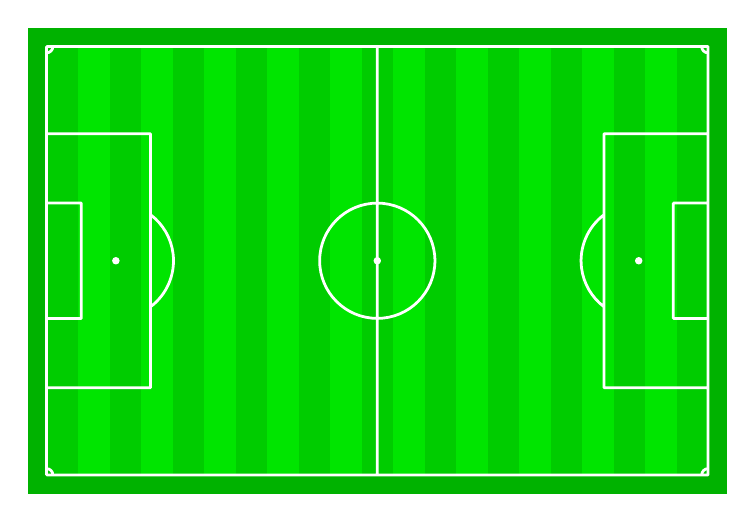
\begin{tikzpicture}[font=\footnotesize,line join=round,line cap=round,>=stealth,scale=0.08,declare function={dai=105; rong=68; bankinh=9.15; khung=7.32; vcam=16.5; vnam=5.5;}]
				 \fill[green!70!black] (0-3,0-3) rectangle (dai+3,rong+3);
				\foreach \i in  {0,2,...,20}{
					\fill[green!80!black] (5*\i,0) rectangle (5*\i+5,68); 
				 }
				\foreach \i  in {0,2,...,18}{
					 \fill[green!90!black] (5*\i+5,0) rectangle (5*\i+10,68);
				} 
				\draw[white,line width=1pt] 
					(0,0) rectangle (dai,rong) 
					 (dai/2,0)--++(0,rong)
					(dai/2,rong/2)  circle (bankinh)
					(0+1,0) arc  (0:90:1)
					 (0,rong-1) arc (-90:0:1)
					(dai,1) arc  (90:180:1)
					(dai,rong-1) arc (-90:-180:1) 
					 (0,rong/2-khung/2-vcam) rectangle (vcam,rong/2+khung/2+vcam)
					(0,rong/2-khung/2-vnam) rectangle  (vnam,rong/2+khung/2+vnam)
					(dai,rong/2-khung/2-vcam) rectangle  (dai-vcam,rong/2+khung/2+vcam)
					(dai,rong/2-khung/2-vnam) rectangle  (dai-vnam,rong/2+khung/2+vnam)
					(11,rong/2)+(-53:bankinh)  arc (-53:53:bankinh)
					 (dai-11,rong/2)+(127:bankinh) arc (127:233:bankinh);
				\fill[white,draw] 
					(dai/2,rong/2) circle (0.5) 
					(11,rong/2) circle  (0.5)
					 (dai-11,rong/2) circle (0.5);
			\end{tikzpicture}
	\end{center}
	 \shortans{3}
	\loigiai{ 
		Từ phương trình mặt cầu, suy ra  mặt cầu có tâm $I(32;50;10)$ và bán kính $R=\sqrt{109}$ (m).\\
		Khoảng cách từ tâm $I$ đến mặt sân  là $\mathrm{d}\left(I,(Oz)\right)=10$.\\
		Suy  ra $IJ=10$ (m).\\
		 Do $M\in(S)$ nên $IM=R=\sqrt{109}$ (m).\\
		Khi đó, khoảng cách từ vị trí $M$ của quả bóng đến điểm $J$ bằng 
		 $$IM=\sqrt{R^2-IJ^2}=\sqrt{\sqrt{109}^2-10^2}=\sqrt{9}=3\,\text{ (m)}.$$
	} 
\end{bt}

% nguồn: Phan2_Lop_12_Hinh_hoc_Chuong_5
\begin{bt}%[2H5H3-4]%[ma:3b19d73e]
	Khi đặt hệ toạ độ $Oxyz$ vào không gian với đơn vị trên trục tính theo ki-lô-mét, người ta thấy rằng một không gian  phủ sóng điện thoại có dạng một hình cầu $(S)$ (tập hợp những điểm nằm trong và nằm trên mặt cầu tương ứng). Biết mặt cầu $(S)$ có phương trình $x^2+y^2+z^2-2x-4y-6z+5=0$. Khoảng cách xa nhất giữa hai điểm thuộc vùng phủ sóng là bao nhiêu ki-lô-mét?
	 \shortans{6}
	 \loigiai{
		Ta có $a=1$,  $b=2$, $c=3$, $d=5$, $R=\sqrt{a^2+b^2+c^2-d}=\sqrt{1^2+2^2+3^2-5}=3$.\\
		Khoảng cách xa nhất giữa hai điểm thuộc vùng phủ sóng bằng đường kính mặt cầu  $$d=2R=2\cdot 3=6.$$
	} 
\end{bt}

% nguồn: Phan2_Lop_12_Hinh_hoc_Chuong_5
\begin{bt}%[2H5H3-4]%[ma:e7cd9db2]
	Trong không gian với hệ trục tọa độ $Oxyz$ (đơn vị trên mỗi trục là mét), một thiết bị phát sóng wifi được đặt tại vị trí $I(3;4;2)$. Vùng phủ sóng của thiết bị là một hình cầu có bán kính $R= 10$ m. Một người sử dụng điện thoại đứng ở vị trí $K(x-7;7;1)$. Sau đó, người đó  di chuyển đến vị trí $H(x+11;7;1)$. Tìm giá trị nguyên của $x$ sao cho cả hai vị trí $K$ và $H$ đều có thể bắt được tín hiệu wifi từ thiết bị.
	 \shortans{1}
	\loigiai{Cả hai vị trí  $K$ và $H$ đều có thể bắt được tín hiệu wifi từ thiết bị khi và chỉ khi
		 \allowdisplaybreaks
		\begin{eqnarray*}
			\heva{&IK \leq 10 \\& IH \leq 10}&\Leftrightarrow&\heva{&(x-10)^2+3^2+(-1)^2 \leq 100 \\& (x+8)^2+3^2+(-1)^2 \leq 100} \\&\Leftrightarrow&\heva{&x^2-20 x+10 \leq 0 \\& x^2+16 x-26 \leq 0} \\&\Leftrightarrow&\heva{&10-3 \sqrt{10} \leq x \leq 10+3 \sqrt{10} \\& -8-3 \sqrt{10} \leq x \leq-8+3 \sqrt{10}}\\&\Leftrightarrow&10-3 \sqrt{10} \leq x \leq-8+3 \sqrt{10}\\&\Leftrightarrow&0{,}5131 \leq x  \leq 1{,}4868.
		\end{eqnarray*}
		Do $x$ nguyên nên  $x=1$.
	} 
\end{bt}

% nguồn: Phan2_Lop_12_Hinh_hoc_Chuong_5
\begin{bt}%[2H5H3-4]%[ma:2ced061a]
	Trong không gian với hệ trục tọa độ $Oxyz$ (đơn vị trên mỗi trục là mét), một ngọn hải đăng được đặt ở vị trí $I(21; 35; 50)$, biết rằng ngọn hải đăng được thiết kế với bán kính phủ sáng là $4$ km. Giả sử người đi biển di chuyển theo một đường thẳng từ vị trí điểm $I$ đến vị trí điểm $D(5\,121; 658; 0)$. Khi người đi biển di chuyển đến điểm $H(a; b; c)$ là điểm cuối cùng trên đoạn $ID$ mà người đi biển có thể nhìn thấy ánh sáng từ ngọn hải đăng. Lúc đó $c$ (cao độ của điểm $H$) có giá trị  bằng bao nhiêu (làm tròn kết quả đến hàng đơn vị)?
	 \shortans{11}
	 \loigiai{
		Mặt cầu phủ sáng  tâm $I$, bán kính $R=4$ (km) $=4\,000$ (m) có phương trình
		\[ 
		(C)\colon (x-21)^2 + (y-35)^2  + (z-50)^2 = 4\,000^2.
		\] 
		 Ta có $\vec{ID} = (5\,100; 623; -50)$.\\
		Phương trình  đường thẳng $ID$ là $ID\colon\heva{&x=21+510t\\ &y=35+623t\\ &z=50-50t.}$\\
		Vì $H$ là điểm cuối  cùng trên đoạn $ID$ mà người đi biển có thể nhìn thấy ánh sáng từ ngọn hải đăng nên $H$ là giao điểm của $ID$ và mặt cầu.\\
		Vì $H\in ID$ nên $H(21+510t;35+623t;50-50t)$.\\ 
		Vì $H\in  (C)$ nên
		\allowdisplaybreaks 
		\begin{eqnarray*}
			&&(21+510t-21)^2 + (35+623t-35)^2  + (50-50t-50)^2 = 4\,000^2\\
			&\Leftrightarrow&  26\,400\,629t^2 = 4\,000^2\\
			&\Leftrightarrow& t\approx \pm  0{,}78.
		\end{eqnarray*}
		Với $t=0{,}78$  thì $z_H\approx 11$, với $t=-0{,}78$ thì $z_H\approx 89$.\\
		Vì người đó di chuyển từ vị trí $I$ về $D$, cao độ giảm dần nên suy ra cao độ cần tìm là  $c=z_H=11$.
	 }
\end{bt}

% nguồn: Phan2_Lop_12_Hinh_hoc_Chuong_5
\begin{bt}%[2H5H3-4]%[ma:b5b59a30]
	Trong không gian $Oxyz$, người  ta muốn thiết kế một lều cắm trại có dạng một phần của mặt cầu bằng phần mềm 3D. Cho phương trình bề mặt của lều là $(S) \colon (x-2)^2+(y-3)^2+(z-1)^2=9$ và sàn của lều nằm trong mặt phẳng $(Oxy)$. Tính bán kính đường tròn sàn của lều (làm tròn đến hàng phần trăm).
	 \shortans{2,83}
	 \loigiai{
		Mặt cầu $(S)$ có tâm  $I(2;3;1)$ và bán kính $R=3$.
		 \\
		Khoảng cách từ tâm $I$ đến $(Oxy)$  là
		$$ 
		d = |z_I| = |1| =  1.
		$$ 
		Bán kính của đáy lều là 
		 $$
		r = \sqrt{R^2 - d^2} = \sqrt{3^2-1^2}  = 2\sqrt{2}
		 \approx 2{,}83.
		$$ 
	} 
\end{bt}

% nguồn: Phan2_Lop_12_Hinh_hoc_Chuong_5
\begin{bt}%[2H5H3-4]%[ma:76c176a7]
	Khi đặt hệ tọa độ $Oxyz$ vào không gian với đơn vị trên trục tính theo ki-lô-mét, người ta thấy rằng một không gian phủ sóng điện thoại có dạng một hình cầu $(S)$ (tập hợp những điểm nằm trong và  nằm trên mặt cầu tương ứng). Biết mặt cầu $(S)$ có phương trình \break $x^2+y^2+z^2-2x-4y-6z+5=0$. Khoảng cách xa nhất giữa hai vùng phủ sóng là bao nhiêu ki-lô-mét?
	\shortans{6} 
	\loigiai{ 
		 Ta có: $x^2+y^2+z^2-2x-4y-6z+5=0\Leftrightarrow (x-1)^2+(y-2)^2+(z-3)^2=3^2$.\\
		Khoảng cách xa nhất giữa hai  điểm thuộc vùng phủ sóng là đường kính của mặt cầu, tức là $6$ km.
	 }
\end{bt}

% nguồn: Phan2_Lop_12_Hinh_hoc_Chuong_5
\begin{bt}%[2H5V3-4]%[ma:c5380468]
	\immini 
	{Một robot khảo sát không gian hoạt động trong môi trường 3D có một cảm biến hình cầu, được lập trình để di chuyển sao cho cảm biến này tiếp xúc tại một điểm  $Q$ trên một bức tường nghiêng có phương trình là mặt phẳng $x + y - z - 3 = 0$ để đo đạc.
	} 
	{\begin{tikzpicture}[font=\footnotesize,scale=0.8]
		 \coordinate (O) at (0,0);
		\draw[teal] (O)--++(60:2) coordinate  (E)--++(8,0) coordinate (F)--++(-120:2)--cycle;
		\path [name path=EF] (E)--(F); 
		 \path[name path=dtron] (3,2) coordinate (J) circle (1.5);
		\path[name intersections={of=dtron  and EF,by={P,Q}}];
		 \draw[teal,fill=white] (3,2) circle (1.5);
		\coordinate (N)  at ($(J)+(20:1.5)$);
		\coordinate (B)  at ($(J)+(80:1.5)$);
		\coordinate (M) at  ($(J)+(-90:1.5)$);
		\coordinate  (K) at ($(M)+(4,0)$);
		\path[name  path=NB](N)--(B);
		\path[name  path=MK](M)--(K);
		\coordinate (I) at  (intersection of M--K and N--B);
		\draw[teal] [dashed]  (J)--(M) node[midway,left]{$R$}
			 (N)--(B)
			(P)--(Q); 
		 \draw[teal] (M)--(I)--(N);
		\draw[teal]  ($(O)+(1,0)$) arc (0:60:1);
		 \node at ($(O)+(24:0.6)$){$Oxy$};
		 \foreach\x/\y in {J/120,N/30,M/-90,B/90,I/0}{
			 \fill (\x) node[shift={(\y:2mm)}]{$\x$} circle (0.05);
		} 
	\end{tikzpicture}
	 }\noindent
	Trong lúc khảo sát, cảm biến luôn phải đi qua hai điểm chuẩn đã cố định sẵn trong không gian là điểm $M(1; 1; 1)$ - \textit{vị trí cảm biến tại lần đo đầu tiên} và điểm $N(-3;-3;-3)$ \textit{vị trí cảm biến tại lần đo tiếp theo}. Để tối ưu hoá phần mềm điều hướng, kỹ sư muốn xác định rằng: Dù cảm biến (hình cầu) có di chuyển sao cho tiếp xúc ở đâu trên  bức tường, điểm tiếp xúc đó luôn nằm trên một đường tròn cố định. Tính bán kính của đường tròn cố định đó, từ đó giúp lập trình robot dò tìm tiếp điểm dễ dàng hơn trong các lần đo tiếp theo.
	\shortans{6} 
	\loigiai{ 
		Đường  thẳng $M N$ có phương trình tham số là $\heva{&x=1+t \\& y=1+t \\& z=1+t.}$\\
		Gọi $I = MN \cap (P)$. khi đó tọa độ điểm $I$ ứng với $t$ thỏa mãn 
		$$1 + t + 1  + t - 1 - t - 3 = 0 \Leftrightarrow t - 2 = 0 \Leftrightarrow t = 2 \Rightarrow I(3; 3; 3) \Rightarrow IM = 2\sqrt{3}, I N=6 \sqrt{3}.$$
		Do mặt cầu $(S)$ đi qua $M$, $N$ và tiếp xúc với đường thẳng  $IQ$ tại điểm $Q$ nên ta có
		 $$IQ^2 = IM \cdot IN = KI^2 - R^2 \Rightarrow IQ^2 = IM \cdot IN = 36 \Leftrightarrow IQ=6.$$
		Vậy $Q$  luôn thuộc đường tròn tâm $I$ bán kính $R = 6$.
	} 
\end{bt}

% nguồn: Phan2_Lop_12_Hinh_hoc_Chuong_5
\begin{bt}%[2H5V3-4]%[ma:d6cd0b0a]
	\immini{Trong không gian với hệ trục tọa độ $Oxyz$ (đơn vị trên mỗi trục là kilômét), đài kiểm soát không lưu sân bay ở vị  trí $O(0; 0; 0)$ và được thiết kế phát hiện máy bay ở khoảng cách tối đa 500 km . Một máy bay đang ở vị trí $A(-1000; -185; 30)$ và chuyển động với vận tốc không đổi theo quỹ đạo là đường thẳng $d$ có vectơ chỉ phương $\vec{u} = (100; 80; 0)$. Tính khoảng cách từ vị trí $A$ đến khi đài kiểm soát không lưu phát hiện được máy bay (đơn vị km, làm tròn kết quả đến hàng đơn vị).
	}{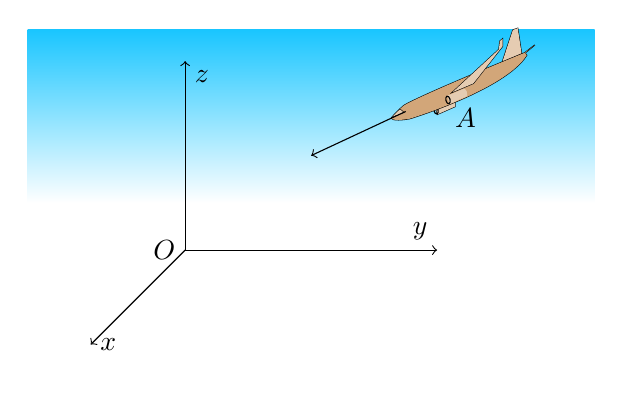
\begin{tikzpicture}[scale=0.8]
		 \definecolor{deepskyblue}{rgb}{0.0,0.75,1.0}
		 \fill[bottom color=white,top color=deepskyblue!90,middle color=white] (-4.5,-3) rectangle (4.5,2.5);
		\tikzset{radar/.pic={ 
		\begin{scope}
			\clip (1.9,2.11) -- +(70:2.5) --  +(-20:2.5)-- cycle;
			\fill[even odd rule] (1.9,2.11) circle (0.5) circle (0.75)  circle (1) circle (1.25)
				circle  (1.5) circle (1.75);
		\end{scope}
		\fill[shift={(25:0.2)}] (1.9,2.11) circle  (0.15);
		\fill (1.02,1.79) -- (1.12,1.6) -- (1.85,2.06).. controls +(162:0.05)  and +(-106:0.05)..
			 (1.81,2.13) -- cycle
			(0.57,2.71).. controls +(-107:0.25)  and +(117:0.25)..
			(0.92,1.56)..  controls +(-62:0.25) and +(158:0.3)..
			(1.6,0.7).. controls +(-173:0.35) and  +(-59:0.7)..
			(0.52,1.36).. controls +(121:0.75) and  +(-150:0.35)..
			(0.57,2.71) -- cycle 
			(1,0.1) -- (0.1,0.1) -- 
			(0.36,1.59).. controls +(-71:0.3) and +(138:0.3).. (0.82,0.9)  -- cycle;
		\draw[line  width=2.5pt] (1.27,1.98).. controls (1.08,2.31) and (0.77,2.77)..
			(0.67,2.71).. controls (0.56,2.65) and (0.81,1.99).. 
			(0.98,1.66).. controls  (1.14,1.33) and (1.55,0.73)..
			(1.66,0.79).. controls (1.77,0.86) and  (1.55,1.42)..
			 (1.41,1.69);
		\fill (0,0) -- (1.1,0) arc  (90:0:0.2)
			-- (-0.2,-0.2) arc (180:90:0.2)--cycle; 
			 }}
		 \tikzset{maybay/.pic={
		\def\D{(-2,-.45)--(-2.36,.24)--(-2.2,.3)--(-1.35,-.25)--cycle;} 
		 \draw \D;
		 \fill[brown!40!] \D;
		\def\Q{ 
			 (.15,-.1)
			..controls +(-140:0.1) and +(140:0.1)..  (.2,-.35)
			--(.8,-.17)--(.7,.07)--cycle; 
		 }
		\draw \Q; 
		\draw[xshift=.5cm] \Q; 
		 \fill[brown!40!,xshift=.5cm] \Q;
		\draw[rotate=-70,xshift=-.23cm,yshift=1.27cm] (.7,-.1)  ellipse (.12cm and 0.07cm);
		\def\T{(-2.1,-.5) 
			..controls +(40:0)  and +(-170:0.7).. (2,.74)
			..controls +(-40:0) and  +(170:0.3).. (2.55,.7)
			..controls +(-150:0) and +(30:.65).. (2.1,.3) 
			..controls +(-150:0) and +(-18:1.25)..  (-2.1,-.6)
			..controls +(90:0) and +(-90:0)..  (-2.1,-.51)
			--(-2.5,-.52)--cycle; 
		} 
		\draw  \T;
		\fill[brown!70!] \T; 
		\def\C{(.5,.05) 
			..controls +(170:0) and +(-10:0).. (-1.48,.12) 
			..controls +(-80:0)  and +(170:0.02).. (-1.65,.3)
			..controls +(180:0) and +(0:0)..  (-1.77,.3)
			..controls +(-80:0) and +(110:0).. (-1.64,.12) 
			..controls +(-35:0)  and +(145:0).. (-.2,-.17)
			--cycle; 
		} 
		\draw \C; 
		\fill[brown!40!] \C; 
		\fill[brown!40!]  \Q;
		\draw[rotate=-70,xshift=-.4cm,yshift=.8cm] (.7,-.1) ellipse  (.12cm and 0.07cm);
		\draw  (2.18,0.73)--(2.5,0.7)--(2.14,0.58)--cycle;
		 \fill[brown!40!](2.18,0.73)--(2.51,0.71)--(2.14,0.57)--cycle;
			 }}
		\path 
			 (2.45,1.65) pic[rotate=35,xscale=-.4,yscale=.4,yslant=-.1]{maybay};
		 \path
			(-2,-1)  coordinate (O)
			 (2.45,1.4) coordinate (A)
			(-3.5,-2.5)  coordinate (x)
			(2,-1) coordinate (y) 
			(-2,2) coordinate  (z);
		 \draw[->] (O)--(x) node[right]{$x$};
		\draw[->] (O)--(y) node [above left]{$y$}; 
		\draw[->] (O)--(z) node  [below right]{$z$};
		\draw[->] (1.5,1.2)--(0,.5); 
		 \draw (O) node[left]{$O$};
		\draw (A) node [below] {$A$}; 
	\end{tikzpicture}
	 }
	\shortans{761} 
	 \loigiai{
		Gọi $M$ là giao điểm của đường thẳng $d$ với  mặt cầu $(S)$ tâm $O$ bán kính $R = 500$ km.\\
		Khi đó, yêu cầu bài toán là tính độ dài  đoạn $AM$.\\
		Ta có $(S)\colon x^2+y^2+z^2=500^2$,  $d \colon \heva{&x = -1000 + 100t\\& y = -185 + 80t \\& z = 30} \Rightarrow AM = 20\sqrt{41}t$.\\
		Khi  đó
		\allowdisplaybreaks 
		\begin{eqnarray*}
			&&(-1000 + 100t)^2  + (-185 + 80t)^2 + 30^2 = 250000 \\
			&\Leftrightarrow& 16400t^2 - 229600t + 785125  = 0\\
			&\Leftrightarrow& 656t^2 - 9184t +  31405 = 0\\
			&\Rightarrow& \hoac{&t =  \dfrac{1148 + \sqrt{30299}}{164} \Rightarrow AM \approx 1032\\&t = \dfrac{1148 - \sqrt{30299}}{164} \Rightarrow AM \approx 761.}
		\end{eqnarray*}
		Vậy  $AM \approx 761$ km.
	} 
\end{bt}

% nguồn: Phan2_Lop_12_Hinh_hoc_Chuong_5
\begin{bt}%[2H5V3-4]%[ma:59ac9c55]
	 \immini
	{Một công ty xây dựng một hệ thống Giám sát môi trường tại khu công nghiệp. Hai cảm biến không dây được đặt tại hai vị trí $A$, $B$ trong không gian $3$ chiều để thu  thấp dữ liệu không khí. Để đảm bảo tín hiệu truyền giữa hai cảm biến ổn định, công ty thiết kế một bóng bảo vệ tín hiệu hình ảnh cầu di động nhưng luôn đi qua cả hai cảm biến $A$ và $B$. Bóng này cần tiếp xúc với mặt đất để đảm bảo tính ổn định.
	}{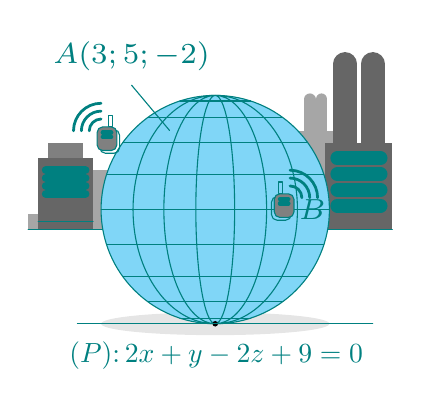
\begin{tikzpicture}[scale=0.5,line join=round,line cap=round,>=stealth]
		 \draw[teal] (-4.75,-0.5) coordinate (T) --(4.5,-0.5) coordinate (P);
		\fill[gray!70] (T) rectangle  ++(1,0.4);
		\fill[gray!70] (T)++(0.5,0) rectangle  ++(3,1.5);
		\fill[gray] (T)++(0.5,0)  rectangle ++(0.9,2.2);
		\fill[black!60]  (T)++(0.25,0) coordinate (dd) rectangle ++(1.4,1.8) coordinate (tt);
		\draw[teal] (dd)++(0,0.2)--++(1.4,0); 
		\foreach \i in  {0,1,2,3}{\draw[teal,line width=3pt](tt)++(-0.2,-0.3-\i*0.2)--++(-1,0);}
		 \fill[gray!70] (P)++(-1.5,0) rectangle ++(-1,2.5) coordinate (pt);
		\draw[teal,line  width=1.5mm,gray!70] (pt)++(0.4,0)--++(0,0.8)
			(pt)++(0.7,0)--++(0,0.8); 
		 \fill[black!60] (P) rectangle ++(-1.7,2.2) coordinate (pt2);
		\draw[teal,line width=3mm,black!60]  (pt2)++(0.5,0)--++(0,2)
			(pt2)++(1.2,0)--++(0,2); 
		\foreach \i in  {0,1,2,3}{\draw[teal,line width=5pt](pt2)++(0.3,-0.4-\i*0.4)--++(1.1,0);}
		 \def\R{2.9}
		\fill[gray!20] (0,-\R) ellipse (\R cm  and 0.1*\R cm);
		\draw[teal,fill=cyan!50] circle  (\R cm);
		\path  (90:\R) coordinate (B)
			(-90:\R) coordinate  (N);
		 \draw[teal] ellipse (0.72*\R cm and \R cm)
			ellipse  (0.45*\R cm and \R cm)
			ellipse (0.17*\R cm and \R  cm);
		\foreach \i in {0,1,...,9}{\draw[teal] (90+\i*18:\R cm)--(90-\i*18:\R  cm);}
		\foreach \diem/\xs in {(-3,1.5)/1,(-2,-0.2)/-1}{ 
			\begin{scope}[xscale=\xs]
			 \path \diem coordinate (tam);
			\draw[teal,rounded  corners=2pt] (tam)++(2pt,-2pt) rectangle +(5mm,6mm);
			\draw[teal,fill=gray,rounded corners=2pt]  (tam) rectangle +(5mm,6mm) coordinate (d);
			\draw[teal] (d)++(-1mm,0) rectangle ++(-1mm,3mm); 
			\draw[teal,line  width=1.5pt] (d)++(-4pt,-4pt)--++(-5mm+8pt,0)
			(d)++(-4pt,-7pt)--++(-5mm+8pt,0); 
			\draw[teal,line width=1pt]  (d)++(-4mm,2mm) arc (90:180:3mm)
			(d)++(-4mm,4mm)  arc (90:180:5mm)
			(d)++(-4mm,6mm) arc (90:180:7mm); 
			\end{scope}
		} 
		\fill  (0,-\R) circle (2pt);
		\draw[teal] (120: 0.8*\R  cm)--++(130:1.5cm) node[above,scale=1.5]{\scriptsize{$A (3; 5; -2)$}}
			 (0.85*\R cm,0) node[scale=1.5]{\scriptsize{$B$}};
		\draw[teal] (-90:\R  cm)++(-3.5,0)--++(7.5,0)++(0,-2mm) node[below left,scale=1]{$(P)\colon 2x+y-2z+9=0$};
	\end{tikzpicture}
	}\noindent 
	Giả sử trong không gian với hệ toạ độ $Oxyz$, toạ độ các điểm là $A(3;5;-2)$, $B(-1;3;2)$ và mặt đất được mô tả bằng mặt phẳng $P(x) \colon 2x+y-2z+9=0$. Trong quá trình mô phỏng, điểm tiếp xúc giữa bóng bảo vệ và mặt đất (gọi là $C$) thay đổi. Kỹ sư cần xác định khoảng cách giữa gốc toạ độ $O(0;0;0)$ đến điểm tiếp xúc $C$ để đánh giá mức độ ảnh hưởng từ vị trí đặt thiết  bị. Gọi $m_{1}$ là giá trị lớn nhất và $m_{2}$ là giá trị nhỏ nhất của độ dài $OC$. Tính giá trị $m_{1}^{2}+m_{2}^{2}$.
	\shortans{76} 
	\loigiai{ 
		\begin{center}
			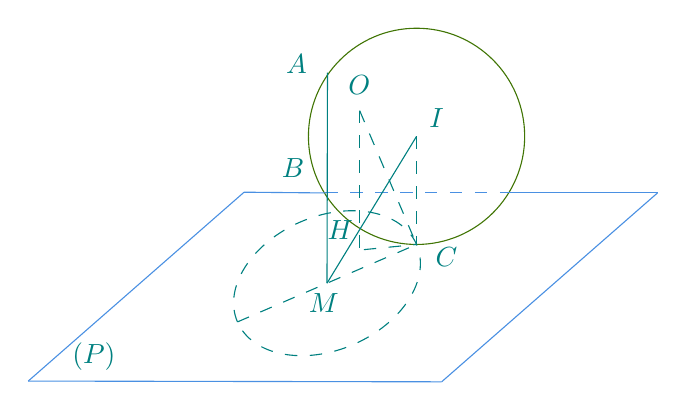
\begin{tikzpicture}[x=0.75pt,y=0.75pt,yscale=-1,xscale=1]
					\draw[teal] [color={rgb,255:red,74; green,144;  blue,226},draw opacity=1] (134,262) -- (333.18,262.36);
					\draw[teal] [color={rgb,255:red,74; green,144; blue,226},draw opacity=1] (333.18,262.36) -- (437.18,171.36); 
					\draw[teal] [color={rgb,255:red,74; green,144; blue,226},draw  opacity=1] (134,262) -- (238,171);
					\draw[teal] [color={rgb,255:red,65; green,117; blue,5},draw opacity=1] (269,144.09).. controls (269,115.32)  and (292.32,92).. (321.09,92).. controls (349.86,92) and (373.18,115.32).. (373.18,144.09).. controls (373.18,172.86) and (349.86,196.18).. (321.09,196.18).. controls (292.32,196.18) and (269,172.86).. (269,144.09) -- cycle;
					\draw[teal] [color={rgb,255:red,74; green,144; blue,226},draw opacity=1] (238,171)  -- (277.18,171.36);
					\draw[teal] [color={rgb,255:red,74; green,144; blue,226},draw opacity=1] [dash pattern={on 4.5pt off  4.5pt}] (277.18,171.36) -- (367.18,171.36);
					\draw[teal] [color={rgb,255:red,74; green,144; blue,226},draw opacity=1] (367.18,171.36)  -- (437.18,171.36);
					\draw[teal] [dash pattern={on 4.5pt off  4.5pt}] (234.81,233.5).. controls (227.76,217.2) and (241.36,195.63).. (265.18,185.32).. controls (289.01,175.02) and (314.04,179.88).. (321.09,196.18).. controls (328.14,212.48) and (314.54,234.06).. (290.72,244.36).. controls (266.89,254.67) and (241.86,249.8).. (234.81,233.5) -- cycle;
					\draw[teal] [dash pattern={on 4.5pt off 4.5pt}] (234.81,233.5)  -- (321.09,196.18);
					 \draw[teal] (278.18,113.36) -- (277.95,214.84);
					\draw[teal] (321.09,144.09) -- (277.95,214.84); 
					\draw[teal] [dash pattern={on 4.5pt off 4.5pt}] (321.09,144.09) -- (321.09,196.18); 
					\draw[teal] [dash pattern={on  4.5pt off 4.5pt}] (293.68,131.68) -- (321.09,196.18);
					\draw[teal] [dash pattern={on 4.5pt off 4.5pt}]  (293.68,131.68) -- (293.68,199.68);
					\draw[teal] [dash pattern={on 4.5pt off  4.5pt}] (295.68,198.68) -- (321.09,196.18);
					\draw[teal] (239.68,207.68); 
					\draw[teal] (154,242.4) node [anchor=north west][inner  sep=0.75pt] {$(P)$};
					\draw[teal] (257,103.4) node [anchor=north west][inner  sep=0.75pt] {$A$};
					\draw[teal] (255,153.4) node [anchor=north  west][inner sep=0.75pt] {$B$};
					\draw[teal]  (326,129.4) node [anchor=north west][inner sep=0.75pt] {$I$};
					\draw[teal] (287,113.4) node [anchor=north west][inner sep=0.75pt]  {$O$};
					 \draw[teal] (329,196.4) node [anchor=north west][inner sep=0.75pt] {$C$};
					\draw[teal] (277,183.4) node [anchor=north west][inner sep=0.75pt]  {$H$};
					\draw[teal] (268,218.4) node [anchor=north west][inner sep=0.75pt] {$M$}; 
				\end{tikzpicture}
		\end{center}
		Dễ thấy  $\heva{&\vec{AB}=(-4;-2;4)=-2(2;1;-2)\\
		&\vec{n}_{P}=(2;1;-2).}$\\ 
		Suy ra $\vec{AB}$, $\vec{n}_{P}$  cùng phương nên $\vec{AB}\perp (P)$, $AB=6$.\\
		Ta có $\mathrm{d}(A,(P))=\dfrac{\left|2\cdot3+5-2\cdot(-2)+9\right|}{\sqrt{2^{2}+1^{2}+(-2)^{2}}}=8$ và $\mathrm{d}(B;(P))=\dfrac{\left|2\cdot(-1)+3-2\cdot(-2)+9\right|}{\sqrt{2^{2}+1^{2}+(-2)^{2}}} = 2$ nên $AB  \cap(P) = M \Rightarrow M$ cố định.\\
		Do $(P)$ tiếp xúc với mặt cầu $(S)$ tại $C$ nên $MC \perp IC$ tại $C$ nên $MA \cdot MB  = MC^{2}$, ta có
		\begin{eqnarray*}
			 \heva{&MA=\mathrm{d}(A,(P))=8\\
			 &MB=\mathrm{d}(B,(P))=2} \Leftrightarrow MC^{2}=16 \Leftrightarrow MC=4.
		\end{eqnarray*}
		Vậy $C$ thuộc đường  tròn tâm $M$ bán kính $r=MC=4$.\\
		 Mặt khác, ta có
		\begin{eqnarray*}
			AB=\heva{&x=3+2t\\ 
			 &y=5+t\\
			&z=-2-2t}\Leftrightarrow M=AB\cap(P) \Rightarrow  M\left( -\dfrac{7}{3};\dfrac{7}{3};\dfrac{10}{3}\right).
		\end{eqnarray*}
		Gọi $H$ là hình chiếu của  $O$ lên mặt phẳng $(P) \Rightarrow \mathrm{d}\left(O,(P)\right)=3, \ OH=\heva{&x=2t\\&y=t\\&z=-2t.}$\\
		Khi đó $H=OM\cap(P) \Leftrightarrow H(-2;-1;2)$, $\ HM = \sqrt{13} <4$ nên $H$ nằm trong đường tròn  tâm $M$ bán kính $r=MC=4$.\\
		 Suy ra $OC = \sqrt{OH^2 + HC^2} = \sqrt{9 + HC^2}$ nên $OC$ đạt GTNN hoặc GTLN $\Leftrightarrow HC$ đạt GTNN hoặc GTLN.
		\begin{eqnarray*}
			\heva{&HC_{\min\limits} = \left| HM-r\right| = 4 - \sqrt{13}\\ &HC_{\max\limits}  = HM+r=4+\sqrt{13}}
			\Rightarrow \heva{&OC_{\min\limits} = \sqrt{9 + \left(4  - \sqrt{13}\right)^2}= m_2\\&OC_{\max\limits} = \sqrt{9 + \left( 4+\sqrt{13}\right) ^{2}} = m_1.}
		\end{eqnarray*}
		Vậy $m_1^2 +  m_2^2 = 76$.
	 }
\end{bt}

% nguồn: Phan2_Lop_12_Hinh_hoc_Chuong_5
\begin{bt}%[2H5V3-4]%[ma:040f5ae6]
	\immini{ 
	Một nhà sản xuất ổ bi đã đặt một mô hình quả cầu khổng lồ trên mái nghiêng của nhà xưởng. Mặt mái có thể được mô tả bằng mặt phẳng $(E)\colon x+2y+2z=10$. Trong đó $A$, $B$, $C$ là giao điểm của mặt phẳng $(E)$ với các trục tọa độ. Một mô hình quả cầu bán kính $r=3$ được đặt tiếp xúc với mặt phẳng $(E)$ tại điểm $C$. Từ $C$ kẻ đường vuông góc với $AB$ tại $F$. Khi thay thế quả cầu, nó lăn trên đường thẳng $CF$ cho đến khi quả cầu vừa tiếp xúc với  mặt phẳng $(Oxy)$ tại $P(a;b;0)$ thì dừng lại. Tính $a+b$.
	 }
	{ 
	\begin{tikzpicture}[scale=0.8,line cap=round,line join=round,font=\footnotesize,>=stealth,declare function={a=4; R=1.2; h=0.6*R; r=1; b=r/4; goc=-130;}]
			 \path
				(0:0)  coordinate (O)
				 (goc:0.6*a) coordinate (A)
				(a,0)  coordinate (B)
				(0,a/2)  coordinate (C)
				($(A)!0.5!(B)$) coordinate (F)++(-10:R)  coordinate (P)
				(R,a/2)  coordinate (M)
				pic[draw,angle radius=1.5mm]  {right angle = C--F--B};
			\draw  (C)--(O)--(B)
				 (O)--(A);
			 \draw[red,line width=1pt](C)--(F)--(P);
			\fill[cyan!70,opacity=0.6] (A)--(B)--(C)--cycle; 
			\draw[line width=0.6pt] (A)--(C)--(B)--cycle; 
			\shade[ball color=yellow!30](M)  circle (R);
			 \draw[->] (B)--++(r,0) node[below]{$y$};
			\draw[->] (A)--++(goc:0.8*r)  node[right]{$x$};
			\draw[->] (C)--++(0,0.8) node[left]{$z$}; 
			 \foreach \x /\gN in {F/-110,A/180,B/-90,C/180,O/50,P/0}
			\fill  (\x) circle (1.2pt)
				 ($(\x)+(\gN:3mm)$) node {$\x$};
		\end{tikzpicture}
	 }
	\shortans{7,8} 
	\loigiai{ 
		Mái nhà xưởng  có phương trình $(E)\colon x+2y+2z=10$.\\
		Giao điểm của $(E)$  với các trục tọa độ:
		\begin{itemize}
			\item Với trục $Ox$,\;$(y=z=0) \Rightarrow  x=10\Rightarrow A(10;0;0)$.
			\item Với trục $Oy$,\;$(x=z=0)  \Rightarrow 2y=10\Rightarrow B(0;5;0)$.
			\item Với trục $Oz$,\;$(x=y=0) \Rightarrow  2z=10\Rightarrow C(0;0;5)$.
		\end{itemize}
		Khi  đó $\vec{AB}=(-10;5;0)$, $AB\colon\heva{&x=10-10t\\&y=5t\\&z=0}\Rightarrow F(10-10t;5t;0)$ \\
		 Điều kiện $CF\perp AB\Leftrightarrow \overrightarrow{CF}\cdot \overrightarrow{AB}=0\Leftrightarrow -100+125t_0=0\Rightarrow t_0=\dfrac{4}{5}
		\Rightarrow  F(2;4;0)$. \\
		Vì quả cầu tiếp xúc với $(E)$ tại $C$ nên $\vec{n}=(1;2;2)$ là vectơ chỉ phương  của đường thẳng đi qua tâm
		quả cầu, khi  đó đường thẳng tìm được là $\heva{&x=s\\&y=2s\\&z=5+2s},\; (s > 0)$.\\
		Khi đó $MC=3\Leftrightarrow s^2+(2s-0)^2+(5+2s-5)^2=3^2\Leftrightarrow 9s^2=9\Leftrightarrow s=1$ suy  ra $M(1;2;7)$. \\
		Quả cầu lăn  theo đường thẳng qua $C$ và $F$, nhận $\vec{CF}=(2;4;-5)$ làm vectơ chỉ phương \\
		Vậy quỹ đạo tâm: $d_M\colon\heva{&x=1+2t\\&y=2+4t\\&z=7-5t},\;  (t\in\mathbb{R})$.\\
		Cuối  cùng quả cầu đặt xuống mặt phẳng $(Oxy)\colon z=0$. \\
		Khi tiếp xúc $(Oxy)\colon z=r=3\Rightarrow 7-5t=3\Rightarrow 5t=4\Rightarrow t=0{,}8$. \\ 
		 Khi đó $P\left(\dfrac{13}{5};\dfrac{26}{5}; 0\right)$ là điểm tiếp xúc với $(Oxy)$. \\
		Vậy $a+b=\dfrac{13}{5}+\dfrac{26}{5}=\dfrac{36}{5}=7{,}8$. 
	 }
\end{bt}

% nguồn: Phan2_Lop_12_Hinh_hoc_Chuong_5
\begin{bt}%[2H5V3-4]%[ma:57e02e27]
	Tại lễ Tri ân và trưởng thành của học sinh khối $12$ của một trường THPT CPV. Kết thúc buổi lễ, một học sinh khối $12$ đại diện cho các bạn thả một khinh khí cầu với khát vọng bay cao và vươn xa. Trong không gian $Oxyz$, mỗi đơn vị ứng với $1$ m, giả sử khinh khí cầu đang ở vị trí có phương trình là $(S)\colon(x-1)^2+(y-2)^2+(z-10)^2=2$. Cùng thời điểm đó có ba chiếc flycam $A$, $B$,  $C$ cách nhau $3$ km, $4$ km, $5$ km và tạo thành một tam giác $ABC$ có ba cạnh tiếp xúc với mặt cầu $(S)$, biết rằng mặt phẳng $(ABC)$ song song với mặt phẳng $(P)\colon 2 x-y+2 z-17=0$ và có phương trình dạng $2 x+a y+b z+c=0$. Tổng giá trị của $T=a+b+c$ bằng bao nhiêu?
	\begin{center}
		\begin{tikzpicture}[line join=round,font=\footnotesize,scale=1,>=stealth]
				 \tikzset{KKC/.pic={
				\fill[yellow!15] (4.391,10.304) 
					.. controls  (-0.128,10.257) and (-0.011,6.648).. (2.353,3.877)
					.. controls (2.676,3.495) and (3.045,3.121)..  (3.46,2.759)
					.. controls (4.391,2.761) and  (4.391,2.76).. (5.321,2.76)
					.. controls (5.732,3.119)  and (6.101,3.493).. (6.424,3.871)
					.. controls  (8.788,6.646) and (8.92,10.252).. (4.39,10.304);
				\fill[cyan!40]  (0.906,8.517)
					 .. controls (0.96,8.565) and (1.119,8.601).. (1.174,8.576)
					.. controls (1.365,8.696) and (1.55,8.74)..  (1.797,8.68)
					.. controls (1.909,8.794) and (2.294,8.834).. (2.67,8.774) 
					.. controls (3.093,8.962) and  (3.52,8.962).. (3.888,8.88)
					.. controls (4.047,8.943) and  (4.586,8.968).. (4.905,8.844)
					.. controls (5.306,8.986) and (5.747,8.932)..  (6.102,8.801)
					.. controls (6.537,8.877) and  (6.773,8.875).. (6.969,8.728)
					.. controls (7.24,8.82) and  (7.457,8.754).. (7.585,8.63)
					.. controls (7.631,8.655)  and (7.758,8.661).. (7.823,8.639)
					.. controls (7.729,8.856) and (7.617,9.015)..  (7.483,9.179)
					.. controls (7.418,9.21) and (7.344,9.222)..  (7.254,9.177)
					 .. controls (7.086,9.306) and (6.908,9.336).. (6.669,9.272)
					..  controls (6.378,9.434) and (6.1,9.431).. (5.823,9.333)
					..  controls (5.468,9.482) and (5.094,9.549).. (4.756,9.421)
					 .. controls (4.565,9.524) and (4.215,9.52).. (4.031,9.427)
					.. controls (3.734,9.544)  and (3.272,9.526).. (2.995,9.384)
					.. controls (2.681,9.437) and (2.331,9.374)..  (2.096,9.25)
					.. controls (1.879,9.294)  and (1.664,9.253).. (1.494,9.138)
					 .. controls (1.433,9.159) and (1.298,9.146).. (1.228,9.092)
					 .. controls (1.087,8.902) and (0.98,8.716).. (0.906,8.516);
				\fill[orange!40] (0.906,8.517) 
					 .. controls (0.96,8.565) and (1.119,8.601).. (1.174,8.576)
					.. controls (1.365,8.696) and (1.55,8.74).. (1.797,8.68) 
					 .. controls (1.909,8.794) and (2.294,8.834).. (2.67,8.774)
					.. controls (3.093,8.962) and (3.52,8.962)..  (3.888,8.88)
					.. controls (4.047,8.943) and (4.586,8.968).. (4.905,8.844) 
					..  controls (5.306,8.986) and (5.747,8.932).. (6.102,8.801)
					.. controls (6.537,8.877) and  (6.773,8.875).. (6.969,8.728)
					.. controls (7.24,8.82)  and (7.457,8.754).. (7.585,8.63)
					.. controls  (7.631,8.655) and (7.758,8.661).. (7.823,8.639)
					..  controls (7.908,8.467) and (7.989,8.169).. (8.014,7.99)
					.. controls (7.946,8.016) and (7.846,8.044)..  (7.751,8.003)
					..  controls (7.635,8.127) and (7.344,8.171).. (7.121,8.109)
					 .. controls (6.88,8.224) and (6.56,8.26).. (6.247,8.187)
					.. controls (5.92,8.313) and  (5.402,8.325).. (5.002,8.209)
					.. controls (4.741,8.33) and (4.084,8.322).. (3.779,8.202) 
					 .. controls (3.358,8.276) and (2.869,8.262).. (2.526,8.12)
					.. controls  (2.158,8.183) and (1.886,8.142).. (1.653,8.021)
					.. controls (1.408,8.061) and  (1.184,8.016).. (1.016,7.902)
					..  controls (0.924,7.92) and (0.819,7.903).. (0.75,7.869)
					.. controls (0.778,8.128) and  (0.817,8.282).. (0.906,8.516);
				\fill[cyan!30]  (1.977,4.347)
					.. controls (2.04,4.311) and (2.183,4.304).. (2.262,4.342) 
					.. controls (2.411,4.302) and (2.64,4.261).. (2.778,4.344) 
					 .. controls (2.952,4.242) and (3.158,4.275).. (3.421,4.361)
					.. controls (3.648,4.275) and (3.766,4.309)..  (4.02,4.417)
					.. controls (4.304,4.278) and (4.52,4.306)..  (4.762,4.437)
					.. controls (5.018,4.302) and (5.162,4.274).. (5.387,4.422) 
					.. controls (5.63,4.305) and  (5.894,4.302).. (6.045,4.406)
					.. controls  (6.23,4.283) and (6.384,4.292).. (6.519,4.343)
					.. controls  (6.565,4.286) and (6.718,4.29).. (6.777,4.312)
					.. controls (6.919,4.502) and (6.988,4.612).. (7.118,4.801) 
					 .. controls (7.033,4.789) and (6.922,4.804).. (6.856,4.855)
					..  controls (6.717,4.803) and (6.535,4.819).. (6.342,4.932)
					.. controls (6.103,4.822) and  (5.856,4.848).. (5.619,4.965)
					.. controls (5.342,4.848) and (5.164,4.839)..  (4.852,4.963)
					.. controls (4.557,4.851) and  (4.246,4.868).. (3.922,4.974)
					.. controls (3.593,4.84) and  (3.404,4.862).. (3.17,4.946)
					.. controls  (2.932,4.847) and (2.679,4.805).. (2.455,4.907)
					.. controls (2.261,4.811)  and (2.079,4.775).. (1.929,4.844)
					.. controls (1.853,4.779) and  (1.723,4.792).. (1.653,4.816)
					.. controls (1.758,4.659)  and (1.794,4.603).. (1.976,4.347);
				 \fill[orange!40] (1.977,4.347)
					.. controls (2.04,4.311) and (2.183,4.304).. (2.262,4.342) 
					..  controls (2.411,4.302) and (2.64,4.261).. (2.778,4.344)
					..  controls (2.952,4.242) and (3.158,4.275).. (3.421,4.361)
					.. controls (3.648,4.275) and  (3.766,4.309).. (4.02,4.417)
					.. controls (4.304,4.278) and  (4.52,4.306).. (4.762,4.437)
					 .. controls (5.018,4.302) and (5.162,4.274).. (5.387,4.422)
					.. controls (5.63,4.305)  and (5.894,4.302).. (6.045,4.406)
					.. controls (6.23,4.283) and (6.384,4.292).. (6.519,4.343) 
					.. controls (6.565,4.286) and (6.718,4.29).. (6.777,4.312) 
					.. controls (6.644,4.14) and (6.581,4.039).. (6.425,3.872) 
					.. controls (6.355,3.827)  and (6.228,3.833).. (6.158,3.865)
					.. controls (6.05,3.808) and  (5.862,3.809).. (5.711,3.877)
					.. controls  (5.54,3.811) and (5.296,3.822).. (5.146,3.905)
					.. controls (4.967,3.833)  and (4.826,3.815).. (4.653,3.889)
					 .. controls (4.511,3.808) and (4.277,3.814).. (4.125,3.887)
					 .. controls (3.989,3.796) and (3.8,3.804).. (3.648,3.875)
					.. controls (3.494,3.799)  and (3.238,3.804).. (3.077,3.874)
					..  controls (2.965,3.82) and (2.742,3.824).. (2.622,3.866)
					.. controls (2.551,3.831) and (2.456,3.823).. (2.352,3.877) 
					.. controls (2.154,4.1) and (2.113,4.156)..  (1.977,4.347);
				\fill[blue!50!black]  (5.32,2.76)
					.. controls  (5.389,2.821) and (5.457,2.881).. (5.525,2.942)
					.. controls (4.754,2.928)  and (4.024,2.929).. (3.256,2.942)
					.. controls (3.324,2.881) and  (3.392,2.821).. (3.46,2.76)--cycle;
				\draw[fill=red!70!cyan]  (5.048,2.237)
					.. controls (5.1,2.413) and (5.213,2.636)..  (5.321,2.76)
					.. controls (4.734,2.76) and (4.043,2.76).. (3.46,2.76) 
					.. controls  (3.563,2.646) and (3.702,2.404).. (3.748,2.225)--cycle
					(4.084,1.094)  rectangle (4.692,1.589)
					 (4.636,1.587)--(5.048,2.237)
					(4.152,1.588)--(3.748,2.225) 
					(4.234,1.588)--(3.917,2.227) 
					(4.29,1.588)--(4.078,2.229) 
					(4.348,1.588)--(4.248,2.229) 
					(4.391,1.588)--(4.391,2.234) 
					(4.441,1.588)--(4.541,2.232) 
					 (4.497,1.588)--(4.71,2.234)
					(4.554,1.588)--(4.873,2.234); 
				\draw (4.394,10.304).. controls (-0.129,10.254) and  (-0.008,6.65).. (2.352,3.879)
					.. controls (2.676,3.496) and  (3.046,3.121).. (3.46,2.76)
					(4.394,10.305).. controls  (-0.468,10.037) and (0.465,5.778).. (3.64,2.761)
					(4.392,10.304).. controls (1.06,10.115) and (0.571,6.86)..  (3.903,2.758)
					 (4.392,10.305).. controls (1.977,9.533) and (1.84,7.077).. (4.23,2.759)
					(4.392,10.305).. controls (3.482,8.56)  and (3.529,6.178).. (4.386,2.759)
					(4.387,10.303).. controls (5.218,8.746)  and (5.331,6.532).. (4.394,2.758)
					 (4.388,10.306).. controls (6.802,9.528) and (6.933,7.075).. (4.552,2.76)
					(4.387,10.304).. controls (7.721,10.115) and (8.214,6.861).. (4.882,2.759) 
					 (4.386,10.303).. controls (9.248,10.036) and (8.311,5.779).. (5.14,2.76)
					(4.388,10.306).. controls (8.917,10.251) and  (8.79,6.647).. (6.424,3.872)
					..  controls (6.101,3.493) and (5.732,3.12).. (5.32,2.759);}}
				\draw (5.5,5.75) coordinate (N)  pic[scale=0.15]{KKC};
				\coordinate  (A) at (3,3);
				\coordinate (B)  at (0,0);
				\coordinate  (C) at (8,0);
				\coordinate  (D) at ($(C)-(B)+(A)$);
				\draw[smooth](B)--(C)--(D)--(A)--(B); 
				\draw[->,line width=1.5](A)--($(A)+(2,0)$); 
				 \draw[->,line width=1.5](A)--($(A)+(0,2)$);
				\draw[->,line width=1.5](A)--($(A)!.4  ! (B)$);
				\foreach \diem  in {D,C,A,B} \fill (\diem) circle (1pt);
				\coordinate [label=left:$A$](M) at  (4.24,5.07);
				\coordinate [label=above:$B$](N)  at (7,6.82);
				 \coordinate [label=below:$C$](P) at (7,3);
				\coordinate [label=right:$(S)$](I) at (6,5); 
				\draw [dashed](6,5)  circle (1);
				\draw[dashed](M)--(N)--(P)--(M); 
				\foreach \diem in {M,N,P,I}  \fill (\diem) circle (1pt);
			\end{tikzpicture}
	\end{center}
	 \shortans{-22}
	\loigiai{Mặt cầu $(S)$ có tâm $I(1;2;10)$,  $R=\sqrt{2}$.\\
		Gọi $(C)$ có bán kính $r$ là đường tròn giao tuyến giữa mặt phẳng $(ABC)$ với mặt cầu $(S)$.\\ 
		Ta có đường tròn $(C)$ nội tiếp  tam giác $(ABC)$.\\
		Vì tam giác $ABC$ có độ dài ba cạnh $3$ km,  $4$ km, $5$ km nên tam giác $ABC$ vuông.\\
		Ta có $S_{ABC}=p \cdot r \Rightarrow r=\dfrac{S_{ABC}}{p}=\dfrac{\dfrac{1}{2} \cdot  3 \cdot 4}{\dfrac{3+4+5}{2}}=1$.\\
		Khoảng cách từ tâm mặt cầu đến mặt phẳng $(ABC)$ là $\mathrm{d}=\sqrt{R^2-r^2}=\sqrt{2-1}=1$.\\ 
		Do mặt phẳng $(ABC)$ song song với $(P)\colon2 x-y+2 z-17=0$ nên phương trình mặt phẳng $(ABC)$ có dạng $(P)\colon 2  x-y+2 z+c=0$ với $c \neq-17$.
		$$\mathrm{d}(I,(ABC))=1  \Leftrightarrow \dfrac{|2\cdot 1-2+2\cdot 10+c|}{\sqrt{2^2+(-1)^2+2^2}}=1 \Leftrightarrow|20+c|=3 \Leftrightarrow\hoac{&c=-17&(\text{loại}) \\& c=-23.}$$
		Vậy $(ABC)\colon 2 x-y+2 z-23=0  \Rightarrow a=-1; b=2; c=-23 \Rightarrow T=a+b+c=-22$.
	 }
\end{bt}

% nguồn: Phan2_Lop_12_Hinh_hoc_Chuong_5
\begin{bt}%[2H5V3-4]%[ma:519e653c]
	Cho một hộp quà hình lập phương có cạnh bằng $10$ cm. Trong hộp có một quả cầu pha lê lớn đặt vừa khít vào hộp sao cho quả cầu tiếp xúc với tất cả các mặt của hộp. Ở $8$ góc của hình lập phương, có $8$ quả cầu pha lê nhỏ cùng tiếp xúc với các mặt hộp và tiếp xúc với quả cầu lớn. Đổ epoxy resin (một loại  keo tổng hợp trong suốt dùng trong thủ công mỹ nghệ) vào đầy hộp để trang trí. Tính thể tích phần keo cần đổ, theo đơn vị lít (làm tròn kết quả đến hàng phần mười).
	\shortans{0,4} 
	 \loigiai{
		Thể tích của khối lập phương là $V_{\text{ lập phương}} =  10^3 = 1\,000$ cm$^3$.\\
		Vì quả cầu lớn tiếp xúc với tất cả các mặt của lập phương nên đường kính của nó bằng cạnh lập phương,  tức là
		$d_{\text{ lớn}} = 10$  (cm) $\Rightarrow r_{\text{ lớn}} = \dfrac{10}{2} = 5$ (cm).\\
		Giả sử bán kính quả cầu nhỏ  là $r$. Mỗi quả cầu nhỏ tiếp xúc với ba mặt hộp và tiếp xúc với quả cầu lớn nên tâm của nó nằm trên đoạn nối từ tâm quả cầu lớn đến một đỉnh của hình lập phương.\\
		Khoảng cách từ tâm quả cầu lớn đến một đỉnh hộp là $R\sqrt{3}$,  còn khoảng cách giữa tâm quả cầu lớn và tâm quả cầu nhỏ là $R+r$.\\
		Để quả cầu nhỏ  tiếp xúc với quả cầu lớn và tiếp xúc với các mặt của hộp
		 \[
		R + r  = \sqrt{3}(R - r)
		\Rightarrow  R + r = \sqrt{3}R - \sqrt{3}r
		\Rightarrow r(1+\sqrt{3}) =  R(\sqrt{3}-1)
		\Rightarrow r = R\cdot\dfrac{\sqrt{3}-1}{1+\sqrt{3}}. 
		 \]
		\begin{center}
			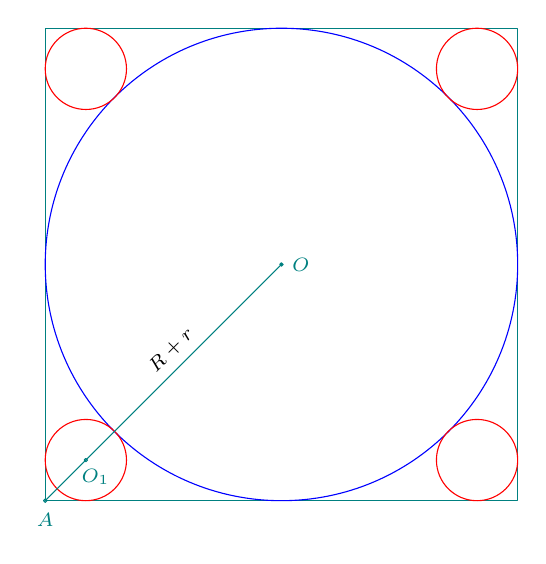
\begin{tikzpicture}[join = round,cap = round,>=stealth,scale=0.6,font=\scriptsize]
					\def\a{10} 
					\def\R{5} 
					 \def\r{0.86}
					 \coordinate (A) at (0,0);
					\coordinate (B)  at (\a,0);
					\coordinate (C)  at (\a,\a);
					\coordinate  (D) at (0,\a);
					 \draw[teal] (A)--(B)--(C)--(D)--cycle;
					\coordinate  (O) at (\a/2,\a/2);
					 \draw[teal,blue] (O) circle (\R);
					\coordinate (O_1)  at (\r,\r);
					\coordinate (O2) at  (\a-\r,\r);
					\coordinate (O3)  at (\a-\r,\a-\r);
					 \coordinate (O4) at (\r,\a-\r);
					\draw[teal,red] (O_1)  circle (\r);
					\draw[teal,red] (O2) circle  (\r);
					\draw[teal,red] (O3)  circle (\r);
					\draw[teal,red] (O4) circle  (\r);
					\foreach \t/\g in {A/-90,O_1/-60,O/0}{ 
						\draw[teal,fill=white] (\t) circle (1pt) node[shift={(\g:7pt)}]{$ \t $}; 
					 }
					\draw[teal]  (A)--(O_1)--(O);
					\path (O_1)--(O)  node[midway,sloped,above]{$R+r$};
				\end{tikzpicture}
		\end{center}
		Rút  gọn
		\[ 
		\dfrac{\sqrt{3}-1}{1+\sqrt{3}} = \dfrac{(\sqrt{3}-1)^2}{(1+\sqrt{3})(\sqrt{3}-1)} =  \dfrac{4-2\sqrt{3}}{2} = 2-\sqrt{3},
		 \]
		nên $r = R(2-\sqrt{3})=  5(2-\sqrt{3})$ cm.\\
		Thể tích quả cầu nhỏ $V_{\text{ nhỏ}} = \dfrac{4}{3}\pi r^3 \approx  \dfrac{4}{3}\pi\left[5(2-\sqrt{3})\right]^3$ cm$^3$.\\
		Tổng thể tích $8$ quả  cầu nhỏ
		$8\cdot V_{\text{ nhỏ}} = 8\cdot \dfrac{4}{3}\pi\left[5(2-\sqrt{3})\right]^3=\dfrac{32\pi}{3}\left[5(2-\sqrt{3})\right]^3$  cm$^3$.\\
		Thể tích quả cầu lớn $V_{\text{ lớn}} = \dfrac{4}{3}\pi(5)^3 = \dfrac{500}{3}\pi $ cm$^3$.\\ 
		Phần thể tích keo cần  đổ
		 \[
		V_{\text{ keo}} = 1\,000 - \dfrac{500}{3}\pi- \dfrac{32\pi}{3}\left[5(2-\sqrt{3})\right]^3 \approx 396\ \mathrm{cm}^3 \approx 0{,}396\ \text{ lít}  \approx 0{,}4\ \text{ lít}.
		 \]
	} 
\end{bt}

% nguồn: Phan2_Lop_12_Hinh_hoc_Chuong_5
\begin{bt}%[2H5V3-4]%[ma:a5cf2680]
	Trong không gian $Oxyz$, (đơn vị trên mỗi trục là mét), một  router phát sóng wifi có đầu thu phát được đặt tại điểm $I(3;-1;2)$ và bán kính phủ sóng wifi là $40\, \mathrm{m}$. Một người đang ở vị trí $A(45;-1;2)$ muốn vào vùng phủ sóng để sử dụng wifi. Để di chuyển theo đường đi ngắn nhất, người đó cần đến điểm $N$ nằm trên ranh giới phủ sóng. Biết $N$ có tọa độ là $(a;b;c)$. Hãy tính giá trị của $a+b+c$.
	\shortans{44} 
	\loigiai{ 
		Vùng phủ sóng wifi có dạng hình cầu tâm $I(3;-1;2)$ và bán  kính $R=40$.\\
		Phương  trình mặt cầu là $(x-3)^2+(y+1)^2+(z-2)^2 = 40^2 = 1600$.\\
		Người  đó đang ở vị trí $A(45;-1;2)$.\\
		Tính khoảng cách từ  $A$ đến $I$:\\
		 $IA = \sqrt{(45-3)^2+(-1-(-1))^2+(2-2)^2} = \sqrt{42^2+0^2+0^2} = \sqrt{42^2} = 42$.\\
	\immini{Vì $IA = 42 > R = 40$ nên điểm $A$ nằm  ngoài vùng phủ sóng.\\
		Để di chuyển theo đường đi ngắn nhất vào vùng phủ sóng, người đó cần di chuyển theo đường thẳng $IA$ và đến  điểm $N$ nằm trên đoạn $IA$ sao cho $N$ nằm trên mặt cầu.\\
		Điểm $N$ là giao điểm của đoạn $IA$ với mặt cầu,  và $N$ gần $A$ nhất.\\
		Ta có $\overrightarrow{IA}  = (45-3;-1-(-1);2-2) = (42;0;0).$\\
		Mà  $\overrightarrow{IN} = \dfrac{R}{IA}\overrightarrow{IA}=
		\dfrac{40}{42}(42;0;0) =  (40;0;0)$.}
		 {
		\begin{tikzpicture}[scale=1,line join=round,line cap=round,>=stealth]
				 \def\bk{2}
				\coordinate  (I) at (0,0);
				\fill (I) circle (1.5pt) node[below left]{$I$}; 
				\draw[blue,name path=semicircle] (I)  ++(0:\bk) arc (0:180:\bk);
				\draw  (-\bk,0)--(\bk,0);
				 \coordinate (A) at (-3,1);
				\fill (A) circle (1.5pt)  node[above left]{$A$};
				\draw[name path=line_AI] (A)--(I); 
				 \path [name intersections={of=semicircle and line_AI,by=N}];
				\fill (N) circle (1.5pt) node[above  left]{$N$};
			\end{tikzpicture}
		 }
		Suy ra 
		$$\heva{&x_N-3 =  40\\& y_N-(-1) = 0 \\&z_N-2 = 0 } \Leftrightarrow \heva{&x_N=43\\&y_N=-1\\&z_N=2.}$$
		Vậy tọa độ điểm  $N$ là $(43;-1;2)$.\\
		Khi đó $a=43, b=-1, c=2$. Suy ra  $a+b+c = 43+(-1)+2 = 44$.
	 }
\end{bt}

% nguồn: Phan2_Lop_12_Hinh_hoc_Chuong_5
\begin{bt}%[2H5V3-4]%[ma:a4909e88]
	\immini{ 
	Để trang trí hội chợ, người ta dùng $2$ quả cầu. Xét trong không gian $Oxyz$, quả cầu thứ nhất có tâm đặt ở vị trí có tọa độ $\left(1;1;2 \right) $ và bán kính bằng $3$ dm; quả cầu thứ hai có tâm đặt ở vị trí có tọa độ $\left( 2;5;-1\right) $ và bán kính bắng $2$ dm. Người ta cố định hai quả cầu bằng hai thanh sắt, một đầu thanh sắt được cố định vào  mỗi quả cầu, đầu còn lại của hai thanh sắt được cố định chung ở một vị trí trên mặt phẳng có phương trình $2x+y+2z+74=0$. Tính tổng độ dài ngắn nhất của hai thanh sắt cần dùng (\textit{kết quả tính theo đơn vị mét và làm tròn đến hàng phần mười}).}
	{\begin{tikzpicture}[line join=round,line cap=round,>=stealth,font=\footnotesize,scale=1]
		 \def\r{1cm}
		 \path
			(0,0) coordinate  (A)
			(6,0.5) coordinate  (B)
			(A)++(-40:1*\r) coordinate  (P)
			 (B)++(-150:0.7*\r) coordinate (Q)
			(A)++(-40:3.5) coordinate  (M);
		\draw  (P)--(M)--(Q);
		\shade[ball color=blue] (A) circle  (\r);
		 \shade[ball color=red] (B) circle (0.7*\r);
		 \foreach \i/\g in {M/-90,P/-90,Q/-90}{\draw (\i) circle (1pt)
			 ($(\i)+(\g:3mm)$) node[scale=1]{$\i$};}
	\end{tikzpicture}
	} 
	 \shortans{49,2}
	\loigiai{ 
		\begin{center}
			\begin{tikzpicture}[line join=round,line cap=round,>=stealth,font=\footnotesize,scale=1]
					 \def\r{1cm}
					 \path
						(0,0) coordinate  (M)
						(-2.3,0)  coordinate (H)
						(40:3.5) coordinate  (I_2)
						(140:3)  coordinate (I_1)
						 (-140:3) coordinate (A)
						 (I_1)++(-40:\r) coordinate (P)
						(I_2)++(-140:0.6*\r)  coordinate (Q);
					 \draw
						(-4,0)--(4,0) 
						(I_1)--(P) node[above,midway,sloped]{$3$}--(M)--(Q)--(I_2) node[above,midway,sloped]{$2$} 
						(I_1)  circle (\r)
						 (I_2) circle (0.6*\r);
					\draw[dashed] (I_1)--(A)--(M); 
					\fill (P) circle (1pt) 
						 (Q) circle (1pt);
					\foreach \i/\g in {M/-60,I_1/90,I_2/90,A/-90,H/-135}{\draw (\i) circle (1pt) 
						($(\i)+(\g:3mm)$)  node[scale=1]{$\i$};}
				\end{tikzpicture}
		\end{center}
		Đặt tên điểm  $I_1\left(1;1;2 \right)$ và $I_2\left( 2;5;-1\right)$.\\
		 Xét hàm số $f(x,y,z)=2x+y+2z+74$.\\
		Ta có $\heva{&f\left(1;1;2 \right)=2\cdot1+1+2\cdot 2+74=81\\&f\left( 2;5;-1\right)=2\cdot2+5+2\cdot (-1)+74=83} \Rightarrow $ Hai điểm $\left(1;1;2 \right)$ và $\left( 2;5;-1\right)$ nằm về  cùng một phía so với mặt phẳng.\\
		Gọi $A$ là  điểm đối xứng với $I_1$ qua mặt phẳng $2x+y+2z+74=0$.\\
		Để tổng độ dài của hai thanh sắt cần dùng là ngắn nhất thì điểm nối hai thanh sắt (Gọi là điểm $M$) phải là  giao điểm của mặt phẳng $2x+y+2z+74=0$ và đường thẳng $AI_2$.\\
		Gọi $H(x;y;z)$ là hình chiếu vuông góc của $I_1$ lên mp $2x+y+2z+74=0$.\\ Khi đó tọa độ điểm $H$ thỏa  mãn hệ phương trình:
		\begin{align*}
			\heva{&x=1  +2t\\&y=1 +t\\&z=2 +2t\\ &2x+y+2z+74=0}\Rightarrow H\left( -17;-8;-16\right).
		\end{align*}
		 Gọi $A\left(x_A;y_A;z_A \right) \Rightarrow \heva{&\dfrac{x_A+1}{2}=-17\\&\dfrac{y_A+1}{2}=-8\\&\dfrac{z_A+2}{2}=-16}\Leftrightarrow \heva{&x_A=-35\\&y_A=-17\\&z_A=-34.}$\\
		Suy ra tọa độ điểm $A(-35;-17;-34)$.\\ 
		Đường thẳng $AI_2$  có $\heva{&\text{ qua điểm } I_2\left( 2;5;-1\right)\\&\text{ vtcp } \vec{AI_2}=\left(37;22;33\right)}\Rightarrow \heva{&x=2+37u \\&y=5+22u\\&z=-1+33u.} $\\
		Do đó tọa độ điểm  $M$ thỏa mãn hệ phương trình:
		\begin{align*}
			\heva{&x=2+37u \\&y=5+22u\\&z=-1+33u\\&2x+y+2z+74=0}\Rightarrow  \heva{&u= \dfrac{-1}{2}\\&x=\dfrac{-33}{2} \\&y=-6\\&z=\dfrac{-35}{2}}\Rightarrow M\left(\dfrac{-33}{2};-6;\dfrac{-35}{2} \right).
		\end{align*}
		Vậy độ dài ngắn nhất của hai thanh sắt cần dùng  là
		\begin{align*}
			I_1M+I_2M- R_1-R_2&=\sqrt{\left( 1+\dfrac{33}{2}\right)^2 +\left( 1+6\right) ^2+\left( 2+\dfrac{35}{2}\right)  ^2} + \sqrt{\left( 2+\dfrac{33}{2}\right)^2 +\left( 5+6\right) ^2+\left( -1+\dfrac{35}{2}\right) ^2}-3-2\\
			&\approx 49{,}2\,\,\text{ dm}. 
		\end{align*}
	} 
\end{bt}

% nguồn: Phan2_Lop_12_Hinh_hoc_Chuong_5
\begin{bt}%[2H5V3-4]%[ma:1ec9c016]
	Công nghệ hỗ trợ trọng tài VAR (Video Assistant Referee) thiết lập một hệ tọa độ $Oxyz$ để theo dõi vị trí của quả bóng $M$. Cho biết $M$ đang nằm trên mặt sân có phương trình $z=0$, đồng thời thuộc mặt cầu $(S):(x-33)^2+(y-50)^2+(z-9)^2=97$ (đơn vị độ dài tính theo mét). Gọi $K$  là hình chiếu vuông góc của tâm $I$ của mặt cầu $(S)$ lên mặt sân. Tính khoảng cách từ vị trí $M$ của quả bóng đến điểm $K$ (đơn vị mét).
	 \shortans{4}
	\begin{center}
		\begin{tikzpicture}[scale=0.4,line join=round,line cap=round,>=stealth]
				 \draw[fill=teal] (0,0) rectangle (17,12);
				\path 
					 (1,11) coordinate (A)
					(16,11)  coordinate (B)
					(1,1)  coordinate (C)
					($(17,0)+(150:4)$) coordinate[label=left:$M$]  (M)
					(17,0) coordinate[label=below right:$K$] (K); 
				 \draw[white,line width=0.3mm] (1,1) rectangle (16,11);
				\draw[white,line width=0.3mm] (1,3) rectangle (4,9); \draw[white,line width=0.3mm] (0.5,5.3)  rectangle (1,6.7); \draw[white,line width=0.3mm] (2.5,7.5) rectangle (1,4.5);
				\draw[white,line width=0.3mm] (4,5) arc (90:270:-0.5 and  -1);
				\draw[white,line  width=0.3mm] (8.5,1)--(8.5,11);
				 \draw[white,line width=0.3mm] (8.5,6) ellipse (2 and 2);
				\draw[white,line width=0.3mm] (13,3) rectangle (16,9); \draw[white,line width=0.3mm] (16.5,5.3) rectangle (16,6.7); \draw[white,line width=0.3mm]  (14.5,7.5) rectangle (16,4.5);
				\draw[white,line  width=0.3mm] (13,5) arc (90:270:0.5 and -1);
				\draw (17,0) circle (4) 
					(M)--(K); 
			\end{tikzpicture}
	\end{center}
	\loigiai{ 
		Mặt cầu $(S)$ có tâm  $I(33,50,9)$ và $R=\sqrt{97}$.\\
		Vì $K$ là hình chiếu vuông góc  của tâm $I$ của mặt cầu $(S)$ lên mặt sân nên $K(33,50,0)$.\\
		Xét tam giác $IKM$ có  $IM^2=IK^2+MK^2$ (định lý Pythagore).\\
		Suy ra  $MK^2=IM^2-MK^2=97-9^2=16\Rightarrow MK=\sqrt{16}=4$.\\
		Vậy khoảng cách từ vị trí $M$ của quả bóng đến điểm $K$  là $4$ mét.
	} 
\end{bt}

% nguồn: Phan2_Lop_12_Hinh_hoc_Chuong_5
\begin{bt}%[2H5V3-4]%[ma:2f4d5313]
	\immini{ 
	Một khinh khí cầu nghiên cứu khí tượng được phóng lên để thu thập dữ liệu trong tầng bình lưu. Khinh khí cầu này có thiết bị định vị sử dụng tín hiệu từ các vệ tinh của công ty $S$ để xác định vị trí trong không gian. Tại thời điểm quan sát,  khí cầu đang bay ở độ cao $50$ km và nhận được tín hiệu từ ba vệ tinh $S$ có toạ độ trong không gian $Oxyz$ (đơn vị: km) như sau: Vệ tinh $A$ tại vị trí $A(103; 204; 62)$, vệ tinh $B$ tại vị trí $B(106; 208; 74)$, vệ tinh $C$ tại vị trí $C(105; 212; 134)$. Từ thời gian truyền tín hiệu, hệ thống xác định rằng khoảng cách từ vị trí $M$ của khinh khí cầu đến các vệ tinh là $MA=13$ km, $MB=26$ km, $MC=85$ km. Tính khoảng cách từ khinh khí cầu đến gốc toạ độ $O$ (làm tròn kết quả đến hàng đơn vị của km).
	}{ 
	\begin{tikzpicture}[scale=0.3,line join=round,line cap=round,>=stealth]
			\clip (-9,-4) rectangle  (9,16);
			 \tikzset{
				 khicau/.pic={
			\begin{scope}
				 \draw[teal] (0,0) -- (-0.45,0).. controls +(180:0.1) and +(-90:1)
					.. (-0.7,1) arc (270:90:0.15) coordinate  (A)
					.. controls +(85:0.1) and +(-90:0.2).. (-0.6,1.8) 
					.. controls +(95:3)  and +(-85:3)..(-5,10.2)
					..  controls +(95:4) and +(180:3)..(0,16)
					 .. controls +(0:3) and +(85:4).. (5,10.2)
					.. controls +(-95:3) and +(85:3)..  (0.6,1.8)
					.. controls  +(-90:0.2) and +(95:0.1).. (0.7,1.3) coordinate (B)
					arc (90:-90:0.15) 
					.. controls +(-90:1) and  +(0:0.1).. (0.45,0)--cycle;
				\def\khuyetnho{(0,0)..  controls +(50:4) and +(-40:5)..(1.95,10.9)
					.. controls  +(-60:5) and +(60:2).. cycle;}
				\fill[shift={(1,3.8)}] \khuyetnho; 
				\fill[shift={(-1,3.8)},xscale=-1]  \khuyetnho;
				\def\khuyetlon{(1.67,0) -- (1.2,0.1).. controls +(120:3) and +(-125:4).. (0.68,11.87)  -- (1.46,11.98).. controls +(-100:5) and +(95:4)..cycle;}
				\fill[shift={(-2,3.7)}] \khuyetlon; 
				\fill[shift={(2,3.7)},xscale=-1] \khuyetlon; 
				\draw[teal,rounded corners=1pt] ($(A)+(0.1,0)$)--($(B)+(-0.1,0)$) -- ++ (97:0.6) coordinate (C) --++(-0.15,0) arc (360:180:0.15) --+(-0.1,0) arc  (360:180:0.15)--++(-0.15,0)--cycle;
				\draw[teal] ($(C)+(95:0.2)$) to[out=90,in=-90] ++(0.1,0.7) 
					to[out=190,in=-10]  ++(-1.2,0) to[out=-90,in=90] ++(0.1,-0.7)
					to[out=-15,in=195]  cycle;
			\end{scope}
				 }}
			\tikzset{ 
				 vetinh/.pic={
			\begin{scope}[color=gray]
				 \fill
					(2.3,9.95).. controls +(-160:0.12) and +(70:0.12).. 
					(0.59,8.22).. controls +(-110:0.4)  and +(-165:0.4)..
					(3.17,5.63).. controls +(22:0.16) and +(-135:0.32).. 
					(3.54,5.94) -- (3.82,6.22) -- (3.98,6.05)  -- (4.16,5.89) -- (3.58,5.31).. controls +(-10:0.8) and +(110:0.8)..
					(5.28,3.62) -- (5.63,3.98) -- (6,4.35) -- (6.32,4.02) -- (5.97,3.66).. controls  +(-133:0.48) and +(63:0)..
					(5.58,3.22).. controls  +(-110:0.4) and +(-165:0.4)..
					(8.18,0.64).. controls +(11:0.16) and +(-136:0.96).. 
					(9.09,1.47).. controls +(46:0.96)  and +(-117:0)..
					(9.94,2.38)..  controls +(75:0.16) and +(-45:1.76)..
					(8.75,3.79).. controls +(135:1.76)  and +(15:0.16)..
					(7.34,4.98).. controls +(-166:0) and +(45:0.32).. 
					(6.98,4.67) -- (6.69,4.38) --  (6.37,4.72)
					 .. controls +(45:0.6) and +(-60:0.2)..
					(6.83,5.64)..  controls +(43:0.8) and +(-45:0.26)..
					(6.86,6.94).. controls  +(135:0.4) and +(45:0.6)..
					 (5.6,6.88).. controls +(150:0.24) and +(45:0.6)..
					(4.78,6.51) -- (4.53,6.26) -- (4.19,6.59).. controls +(47:0.48)  and +(-104:0)..
					(4.93,7.39)..  controls +(70:0.16) and +(-45:1.76)..
					(3.78,8.78).. controls +(136:1.12) and +(-18:0).. 
					(2.56,9.95)..  controls +(153:0.16) and +(27:0.16)..
					 (2.3,9.95) --cycle;
				 \foreach \luc in {0,0.96,1.92,6.8,7.76,8.72}{
					 \path[fill=white,rounded corners,shift={(-45:\luc)}] (2.88,8.78) -- (2.45,8.35) -- (1.98,8.8) -- (2.43,9.23) --cycle
					[shift={(-135:1)}] (2.88,8.78) -- (2.45,8.35)  -- (1.98,8.8) -- (2.43,9.23) --cycle;
				 }
				\fill (3.58,5.31).. controls +(-10:0.8)  and +(110:0.8)..
					(5.28,3.62)  -- (6.37,4.72)
					.. controls +(45:0.6) and +(-60:0.2).. 
					(6.83,5.64).. controls  +(43:0.8) and +(-45:0.26)..
					(6.86,6.94).. controls +(135:0.4)  and +(45:0.6)..
					(5.6,6.88).. controls +(150:0.24) and +(45:0.6).. 
					(4.78,6.51) -- cycle; 
				\fill (1.25,4.93).. controls  +(-120:0.16) and +(106:0.16)..
					(1.26,4.38).. controls +(-71:0.32)  and +(126:0.48)..
					(1.89,3.28) -- (2,3.12) --(2.24,3.54)..  controls +(90:0) and +(-90:0.16)..
					(1.73,4.37).. controls +(90:0.16) and +(147:0.48).. 
					(2.48,4.18).. controls +(-33:0.64)  and +(124:0.64)..
					(4.11,2.56).. controls  +(-56:0.48) and +(0:0.16)..
					(4.34,1.78).. controls +(180:0.16)  and +(0:0)..
					(3.49,2.27) -- 
					(3.12,2.06).. controls +(-45:0.8) and  +(-150:0.4)..
					(4.9,1.3).. controls +(25:0.4) and  +(-50:1.2)..
					(4.69,4.02).. controls +(125:0.32) and +(-38:0.32).. 
					(4.02,4.7).. controls +(140:1)  and +(65:0.64).. cycle;
				\fill (2.77,3.33)  --
					(2.22,2.42).. controls +(0:0)  and +(-45:0)..
					(2.19,2.43).. controls +(135:0) and +(-18:0).. 
					(2.06,2.48).. controls +(167:0.32) and  +(90:0.32)..
					(1.52,2.03).. controls +(-90:0.32) and +(180:0.32).. 
					(1.98,1.57).. controls +(0:0.4) and +(-55:0.28).. 
					(2.4,2.26)  --
					(3.31,2.85).. controls +(39:0.16) and  +(-45:0.16)..
					(3.18,3.23).. controls +(135:0.32)  and +(54:0.16)..
					(2.77,3.33)  --cycle;
				\fill[gray] (0.72,2.16).. controls  +(-143:0.16) and +(102:0.16)..
					(0.67,1.47).. controls +(-77:0.48) and +(174:0.48).. 
					(1.55,0.7).. controls +(-6:0.16) and  +(-162:0.16)..
					(2.06,0.74)..  controls +(27:0) and +(-53:0)..
					 (2.11,0.91).. controls +(170:0.2) and +(-40:0.2)..
					 (1.31,1.15).. controls +(160:0.2) and +(-85:0.4)..
					(0.88,2.16).. controls  +(162:0) and +(34:0)..
					 (0.72,2.16) -- cycle
					(0.03,2.11).. controls  +(-119:0.16) and +(105:0.32)..
					(0,1.17).. controls +(-76:0.48) and  +(153:0.48)..
					(0.75,0.18).. controls +(-35:0.32) and +(195:0.4).. 
					(2.08,0.08) --  (2.09,0.3).. controls +(-174:0.16) and +(-17:0.16)..
					(1.28,0.35).. controls +(163:0.32)  and +(-63:0.32)..
					(0.42,1.07).. controls +(120:0.4) and  +(-90:0)..
					(0.24,2.11).. controls +(124:0) and +(63:0).. 
					(0.03,2.11)  --cycle;
			\end{scope}
				}} 
		\fill[fill=gray!20] (-9,-2) to[bend left=0.8cm] (9,-2)--++(0,-2)--++(-19,0)--cycle;
	\draw[teal] (-9,-2) to[bend left=0.8cm] (9,-2);
	 \path (0,4.3) coordinate (tam);
	\pic[xscale=0.2,yscale=0.15] at (0,-1) [pic  type = khicau];
	\pic[scale=0.1,rotate=4] at (-6.8,11)  [pic type = vetinh];
	\pic[scale=0.1,rotate=4] at (5.5,5.2) [pic type =  vetinh];
	\pic[scale=0.1,rotate=4] at (3,12) [pic type  = vetinh];
	 \draw[teal] (tam)++(-5:2.7)--++(30:3cm) node[midway,below right]{$85$ km};
	\draw[teal] (tam)++(58:3)--++(70:5.5cm) node[midway,right]{$26$  km};
	\draw[teal]  (tam)++(105:2.7)--++(132:6cm) node[midway,below left]{$13$ km};
	\end{tikzpicture}
	} 
	 \shortans{229}
	\loigiai{ 
		Do  khinh khí cầu có độ cao $50$ km nên suy ra $M(x;y;50)$.\\
		Theo giả thiết, ta có 
		 \allowdisplaybreaks
		\begin{eqnarray*}
			\heva{& MA=13\\& MB=26\\& MC=85}&\Leftrightarrow  & \heva{& (x-103)^2+(y-204)^2+(50-62)^2=13^2\\& (x-106)^2+(y-208)^2+(50-74)^2=26^2\\& (x-105)^2+(y-212)^2+(50-134)^2=85^2}\\
			&\Leftrightarrow & \heva{&  x^2+y^2-206x-408y=-52\,200\\& x^2+y^2-212x-416y=-54\,400\\& x^2+y^2-210x-424y=-55\,800}\Leftrightarrow\heva{& x^2+y^2=50\,000\\& x=100\\& y=200.}
		\end{eqnarray*}
		Vậy $M(100;200;50)$, suy ra khoảng cách từ khinh khí cầu đến gốc toạ độ  $O$ là
		$$OM=\sqrt{100^2+200^2+50^2}=50\sqrt{21}\approx  229 \text{ km}.$$
	 }
\end{bt}

% nguồn: Phan2_Lop_12_Hinh_hoc_Chuong_5
\begin{bt}%[2H5V3-4]%[ma:809e810a]
	Khi gắn hệ tọa độ $Oxyz$ (đơn vị trên mỗi trục tính theo kilômét) vào không gian, người ta thấy rằng một không gian phủ sóng điện thoại có dạng một hình cầu $(S)$ (tập hợp những  điểm nằm trên và nằm trong mặt cầu tương ứng). Biết mặt cầu có phương trình $x^2+y^2+z^2-4x-6y-2z+5=0$. Khoảng cách xa nhất giữa hai điểm thuộc vùng phủ sóng là bao nhiêu kilômét?
	 \shortans{6}
	\loigiai{ 
		Mặt cầu  $(S)$ có tâm $I(2;3;1)$ và bán kính $R=\sqrt{2^2+3^2+1^2-5}=3$.\\
		Gọi $A$, $B$ là hai điểm thuộc vùng phủ sóng.\\ 
		Khi đó $A$, $B$ có khoảng cách xa nhất khi đoạn $AB$ là đường  kính của mặt cầu.\\
		Vậy khoảng cách xa  nhất giữa hai điểm thuộc vùng phủ sóng là $6$ kilômét.
	 }
\end{bt}

% nguồn: Phan2_Lop_12_Hinh_hoc_Chuong_5
\begin{bt}%[2H5V3-4]%[ma:517d0453]
	 \immini{
	Một bồn chứa khí hình cầu $(K)$ có đường kính $10$\,m tiếp xúc trực tiếp với một bức tường thẳng đứng tại điểm $T(-6;0;5)$. Bồn được che chắn bằng một tấm chắn nghiêng, cố định xuống mặt  đất tại các điểm $A(0;16{,}25;0)$ và $B(12;16{,}25;0)$, đồng thời được chống đỡ bởi các thanh thẳng đứng tại các điểm $C(0;5;15)$ và $D(12;5;15)$ (tham khảo hình vẽ bên). Tính khoảng cách an toàn giữa tấm chắn $E$ và mặt cầu $(K)$ (đơn vị mét).
	} 
	 {
	\begin{tikzpicture}[scale=0.8,font=\footnotesize,line join=round,line cap=round,>=stealth]
			\tikzset{declare function={a=5; b=0.65*a; goc=45;  h=0.85*a; r=1;}}
			\path (0:0) coordinate (O) 
				 (a,0) coordinate (C1)
				(goc:b) coordinate (A1) ++(a,0) coordinate (B1) 
				(0,h)  coordinate (S)
				($(O)!0.5!(A1)$) coordinate (I1)++(r,r) coordinate  (I)
				 (I1)++(0,r) coordinate (T)
				(I1)++(r,0)  coordinate (It)
				(I1)++(0,1)  coordinate (I1y)
				(I)++(goc+25:r) coordinate  (K)
				($(K)!-0.4!(I)$) coordinate (E) 
				($(K)!1!90:(I)$) coordinate (Et) 
				(intersection of E--Et and  I1--It) coordinate (H)
				(intersection of  E--Et and I1--I1y) coordinate (St)
				(H)++(goc-180:b/2) coordinate (A) 
				($2*(H)-(A)$)  coordinate (B)
				(St)++(goc-180:b/2) coordinate  (M)
				(r,0) coordinate (Cx)++(0,1)  coordinate (Ct)
				($(A1)+(r,0)$)  coordinate (C2)
				(intersection of Cx--Ct and  M--A) coordinate (C)++(goc:b) coordinate (D);
			\draw[gray!70,dashed,line  width=2pt](D)--(C2);
			 \draw[dashed] (K)--(E)
				(O)--(A1) 
				(C)--(D); 
			\fill[pink!70,opacity=0.5] (S)--(O)--(A1)--($(S)+(A1)-(O)$)--cycle; 
			\fill[brown!40,opacity=0.5]  (O)--(A1)--(B1)--(C1)--cycle;
			\shade[ball color=yellow!30,opacity=0.7](I)  circle (r);
			 \draw[fill=cyan!40,opacity=0.5] (M)--(A)--(B)--($(M)+(B)-(A)$)--cycle;
			\draw[gray!90,line  width=2pt](C)--(Cx);
			\fill (K) circle (1pt); 
			\foreach \x /\gN  in {A/-90,B/0,E/90,C/200,D/30,T/180}
			 \fill (\x) circle (1pt)
				($(\x)+(\gN:2.5mm)$) node  {$\x$};
			\draw[->] (C1)--++(r,0) node[below]{$y$}; 
			\draw[->]  (O)--++(goc-180:0.8*r) node[right]{$x$};
			\draw[->] (S)--++(0,0.8) node[left]{$z$}; 
			 \draw (S)--(O)--(C1);
		\end{tikzpicture}
	 }
	\shortans{1} 
	\loigiai{ 
		Bức tường thẳng đứng nằm  trong mặt phẳng $y=0$. \\
		Mặt cầu bán kính $r=5$\,m, tiếp xúc tường  tại $T(-6;0;5)\Rightarrow$ tâm $I(-6;5;5)$. \\
		Tấm  chắn hiện tại $E$ đi qua $A(0;16{,}25;0)$, $B(-12;16{,}25;0)$, $C(0;5;15)$ và $D(-12;5;15)$. \\
		Phương trình mặt cầu  $(K)\colon (x+6)^2+(y-5)^2+(z-5)^2=25$. \\
		Phương  trình mặt phẳng chứa tấm chắn $(E)$ \\
		 $\vec{AB}=(-12;0;0)$, $\vec{AC}=(0;-11,25;15)\Rightarrow\vec{n}=\dfrac{1}{3}\left[\overrightarrow{AB},\overrightarrow{AC}\right]=(0;4;3)$. \\
		 Do đó mặt phẳng $(E)\colon 4y+3z-65=0$. \\
		\lq\lq Khoảng cách an toàn\rq\rq~giữa $(E)$ và mặt cầu $(K)$ là $d=\mathrm{d}(O,(E))=\dfrac{|4\cdot5+3\cdot5-65|}{\sqrt{4^2+3^2}}=\dfrac{30}{5}=6$\,m.  \\
		Khoảng hở giữa bề mặt khối cầu  $(K)$ và $(E)$ là $d-r=6-5=1$\,(m).
	 }
\end{bt}

% nguồn: Phan2_Lop_12_Hinh_hoc_Chuong_5
\begin{bt}%[2H5V3-4]%[ma:165c053c]
	Hệ thống định vị toàn cầu GPS là một hệ thống cho phép xác định chính xác vị trí của một vật trong không gian. Cách thức họat động của GPS như sau: Trong cùng một thời điểm, vị trí $M$ của một vật sẽ được xác định bằng $4$ vệ tinh cho trước, các vệ tinh này có gắn máy thu tín hiệu, bằng cách so sánh thời gian từ lúc tín hiệu được phát đi với thời gian nhận tín hiệu phản hồi thì sẽ xác định được khoảng cách từ các vệ tinh đến vị trí $M$. Như vậy, vị trí $M$ là giao điểm của 4 mặt cầu có tâm là $4$ vệ tinh đã cho. Giả sử trong không gian $Oxyz$, $4$ vệ tinh có tọa độ là $A(-1;6;3)$, $B(4;8;1)$, $C(9;6;7)$, $D(-15;18;7)$. Biết khoảng cách từ $M$ đến các vệ tinh lần lượt là $MA=6$, $MB=7$, $MC=12$, $MD=24$. Khi đó  tọa độ điểm $M\left(x_M;y_M;z_M\right)$. Tính giá trị biểu thức $T=x_M+y_M+z_M$.
	 \shortans{2}
	\loigiai{ 
		Gọi  $M(a;b;c)$. Khi đó ta có\\
		$(a+1)^2+(b-6)^2+(c-3)^2=36\Leftrightarrow  a^2+b^2+c^2+2a-12b-6c+10=0.\hfill(1)$\\
		$(a-4)^2+(b-8)^2+(c-1)^2=49\Leftrightarrow a^2+b^2+c^2-8a-16b-2c+32=0.\hfill(2)$\\ 
		$(a-9)^2+(b-6)^2+(c-7)^2=144\Leftrightarrow  a^2+b^2+c^2-18a-12b-14c+22=0.\hfill(3)$\\
		 $(a+15)^2+(b-18)^2+(c-7)^2=576\Leftrightarrow a^2+b^2+c^2+30a-36b-14c+22=0.\hfill(4)$\\
		Giải  hệ gồm $4$ phương trình trên ta được $a=1$; $b=2$; $c=-1$ nên $M(1;2;-1)$.\\
		 Vậy $T=1+2+(-1)=2$.
	 }
\end{bt}

% nguồn: Phan2_Lop_12_Hinh_hoc_Chuong_5
\begin{bt}%[2H5V3-4]%[ma:8aaa0e59]
	Trong không gian $Oxyz$, đơn vị trên mỗi trục là $2\,000$\,km, người  ta mô phỏng bề mặt Hỏa tinh dưới dạng mặt cầu $(S)\colon x^2+y^2+z^2-2x-2y-2z=0$; một robot do thám được gởi đến bởi các nhà khoa hoạc từ trái đất đang ở vị trí $A(2; 2; 0)$. Người ta cần đặt một thiết bị nhận tín hiệu từ robot ở vị trí $B$ thuộc bề mặt sao Hỏa sao cho $B$ có hoành độ dương và tam giác $OAB$ đều. Tìm khoảng cách thực tế từ vị trí $B$ đến vị trí $C(0; 2; 0)$, nơi đáp xuống của tàu vũ trụ (làm tròn đến hàng phần trăm của nghìn km).
	 \shortans{6,93}
	\loigiai{Gọi $B(x; y; z)$ thuộc $(S)$ với $x  > 0$ và $H$ trung điểm $OA\Rightarrow H(1; 1; 0)$.\\
		 Gọi $(P)$ là mặt phẳng trung trực đoạn $OA$, do đó $(P)$ đi qua trung điểm $H(1; 1; 0)$ của đoạn $OA$ và nhận $\overrightarrow{OA}=(2; 2; 0)$ làm vectơ pháp tuyến. \\
		Suy ra  $(P)\colon 2(x-1)+2(y-1)=0\Leftrightarrow x+y-2=0$.\\
		Theo giả thiết  \allowdisplaybreaks
		\begin{eqnarray*}
			 &&\heva{&OB=AB\\&OB=OA\\&B\in(S)}
			\Leftrightarrow\heva{&B\in(P) \\&OB^2=OA^2\\&B\in(S)}  \Leftrightarrow\heva{&x+y-2=0\\&x^2+y^2+z^2=8\\&x^2+y^2+z^2-2x-2y-2z=0}\\
			&\Leftrightarrow& \heva{&x+y=2 \\&{x  ^ 2+y ^ 2+z ^ 2=8} \\&{2x+2y+2z=8}} \Leftrightarrow \heva{&{x+y=2} \\&{x^2+y^2=4} \\&{z=2}}
			\Leftrightarrow \heva{&{x+y=2} \\&(x+y)^2-2xy=4  \\& {z=2}}
			\Leftrightarrow \heva{&x+y=2\\&x y=0\\&z=2.} 
		\end{eqnarray*}
		Ta tìm được $\heva{&x=2\\&y=0\\&z=2} \Rightarrow B(2; 0; 2)$, (do $x  > 0$). Do đó $BC=\sqrt{2^2+2^2+2^2}=2\sqrt{3}$.\\
		Khoảng cách thực tế là $2\sqrt{3} \cdot 2\approx 6{,}93$  (nghìn km).
	} 
\end{bt}

% nguồn: Phan2_Lop_12_Hinh_hoc_Chuong_5
\begin{bt}%[2H5V3-4]%[ma:2244cd7f]
	\immini{ 
	Bán kính Trái Đất lấy bằng $6\,400$ km, khi gắn hệ trục toạ độ $Oxyz$ thì bề mặt Trái Đất  là mặt cầu có phương trình $x^2+y^2+z^2=64$, đường xích đạo nằm trên mặt phẳng $(Oxy)$. Một tàu vũ trụ X rời khỏi bề mặt Trái Đất theo phương tiếp tuyến với đường tròn vĩ tuyến tại điểm $A(5;\sqrt{23};4)$, với giả thiết rằng sau khi rời khỏi bề mặt Trái Đất tàu vũ trụ X bay theo quỹ đạo thẳng với tốc độ không đổi bằng $8$ km/s. Hỏi sau đúng $20$ phút kể từ khi rời khỏi bề mặt Trái Đất thì khoảng cách từ tàu vũ trụ đến một điểm trên đường tròn xích đạo ngắn nhất bằng bao nhiêu kilomet (làm tròn kết quả đến hàng đơn vị)?
	}{ 
	\begin{tikzpicture}[scale=0.6,line join=round,line cap=round,>=stealth]
			\tikzset{ 
				declare function={ 
				r=4; ry=0.8; d=1.5; ra=sqrt (4^2-1.5^2); rb=0.5; 
				 }}
			 \path
				 (0,0) coordinate (O)
				++(0:r)  coordinate (K)
				($(O)+(90:d)$)  coordinate (H)
				($(O)!1.6!(K)$) coordinate (N) 
				($(H)+(N)-(O)$) coordinate  (M)
				($(H)+(60:ra and rb)$) coordinate  (A)
				($(H)+(0:ra  and rb)$) coordinate (B);
			\draw (O) circle  (r)
				(A)--(M) 
				(K)  arc (0:-180:r and ry)
				(B) arc (0:-180:ra  and rb);
			\draw [dashed] (O)--(H)--(A) 
				 (K) arc (0:180:r and ry)
				 (B) arc (0:180:ra and rb);
			 \foreach \a/\b/\c in {H/A/M}
			\draw pic[draw,angle radius=2mm] {right angle = \a--\b--\c}; 
			\foreach \i/\g in {O/-90,M/90,A/90} 
			\fill  (\i) circle (1pt)+(\g:0.35) node[scale=1]{$\i$};
		\end{tikzpicture}
	} 
	 \shortans{5674}
	 \loigiai{
		\begin{center}
			\begin{tikzpicture}[scale=0.8,line join=round,line cap=round,>=stealth]
					\tikzset{ 
						declare  function={
						r=4; ry=0.8; d=1.5;  ra=sqrt (4^2-1.5^2); rb=0.5;
						}} 
					\path 
						(0,0)  coordinate (O)
						++(0:r) coordinate  (K)
						 ($(O)+(90:d)$) coordinate (H)
						($(O)!1.6!(K)$) coordinate  (N)
						($(H)+(N)-(O)$) coordinate  (M)
						($(H)+(60:ra and rb)$) coordinate  (A)
						($(H)+(0:ra and rb)$)  coordinate (B);
					 \draw (O) circle (r)
						(K) arc  (0:-180:r and ry)
						(B) arc (0:-180:ra and  rb);
					\draw [dashed] (O)--(H)--(A) 
						(O)--(K) node[pos=0.5,below]{$R$} 
						(H)--(B)  node[pos=0.5,below]{$r$}
						(K)  arc (0:180:r and ry)
						(B) arc (0:180:ra and  rb);
					\draw  (B)--(M)--(A)
						(M)--(N)--(K) 
						 (M)--(K);
					\foreach \a/\b/\c  in {H/A/M,K/N/M}
					 \draw pic[draw,angle radius=2mm] {right angle = \a--\b--\c};
					\foreach \i/\g in {O/-90,K/-40,H/180,M/90,N/-90,A/90} 
					\fill  (\i) circle (1pt)+(\g:0.35) node[scale=1]{$\i$};
				\end{tikzpicture}
		\end{center}
		Ta có $R=8$ đơn vị ứng với $6\,400$ km, thì $1$  đơn vị ứng với $\dfrac{6\,400}{8}= 800$ km.\\
		Đường tròn vĩ tuyến tại điểm $A(5;\sqrt{23};4)$ có tâm là  $H(0;0;4)$.\\
		Bán kính $r  =HA= \sqrt{R^2-OH^2} = \sqrt{64-16} = 4\sqrt{3}$.\\
		Quãng  đường tàu vũ trụ bay được\\
		\centerline {$AM = v \cdot t = 8\cdot 20\cdot 60= 9\,600$ km $= 12$  đơn vị.}\\
		Gọi $N$ là  hình chiếu $M$ lên mặt phẳng xích đạo.\\
		Ta có  $MN=OH=4$; $ON=HM=\sqrt{AH^2+AM^2}= 8\sqrt{3}$.\\
		Gọi $K$ là điểm bất kỳ  trên đường xích đạo, ta có\\
		$MK^2=MN^2+KN^2=16+KN^2$.\\ 
		Suy ra $MK$ nhỏ nhất khi $KN$ nhỏ  nhất.\\
		$KN\ge ON-OK\Rightarrow  KN_{min}=ON-R=8\sqrt{3}-8$.\\
		$MK_{min}=\sqrt{MN^2+KN_{min}^2}=\sqrt{4^2+\left(8\sqrt{3}-8\right)^2}$  (đơn vị).\\
		Khoảng cách ngắn nhất cần tìm là $MK_{min}\cdot 800\approx 5\,674$  (km).
	 }
\end{bt}

% nguồn: Phan2_Lop_12_Hinh_hoc_Chuong_5
\begin{bt}%[2H5V3-4]%[ma:5a295d1f]
	 \immini{
	Trong không gian $Oxyz$, mô hình của trái đất là một hình cầu có tâm trái  đất là gốc tọa độ. Giả sử tại một thời điểm, một thiết bị GPS ở vị trí $P(a;b;c)$ cách tâm trái đất $1$\,km và xác định được khoảng cách từ nó tới ba vệ tinh $A$, $B$, $C$ tương ứng là $\sqrt{5}$, $\sqrt{2}$, $2$. Tại thời điểm đó các vệ tinh trên ở vị trí có tọa độ là $A(2;0;0)$, $B(0;2;0)$, $C\left(0;\dfrac{11}{4};\dfrac{\sqrt{7}}{4}\right)$. Tính $a+b+c$ (làm tròn đến hàng phần trăm).
	 }{
	 }
	 \shortans{1,41}
	\loigiai{ 
		Vì thiết bị GPS ở vị trí $P(a;b;c)$ nằm trên mặt  cầu tâm $O$ bán kính $R=1$ nên ta có \[a^2+b^2+c^2=1.\quad (1)\]
		Theo giả thiết, ta  có
		\begin{itemize}
			 \item $PA^2=(a-2)^2+b^2+c^2=\left(\sqrt{5}\right)^2 \Leftrightarrow a^2-4a+4+b^2+c^2=5$.
			\item $PB^2=a^2+(b-2)^2+c^2=\left(\sqrt{2}\right)^2  \Leftrightarrow a^2+b^2-4b+4+c^2=2$.
		\end{itemize}
		Thay $a^2+b^2+c^2=1$ vào  các biểu thức trên, ta được
		\begin{itemize}
			\item $1-4a+4=5 \Leftrightarrow 5-4a=5  \Leftrightarrow a=0$.
			\item $1-4b+4=2 \Leftrightarrow  5-4b=2 \Leftrightarrow 4b=3 \Leftrightarrow b=\dfrac{3}{4}$.
		\end{itemize}
		Thay $a=0$ và $b=\dfrac{3}{4}$ vào phương trình mặt cầu: 
		\[0^2+\left(\dfrac{3}{4}\right)^2+c^2=1 \Leftrightarrow  c^2=1-\dfrac{9}{16}=\dfrac{7}{16}\]
		Lại  có
		 \[PC^2=a^2+\left(b-\dfrac{11}{4}\right)^2+\left(c-\dfrac{\sqrt{7}}{4}\right)^2=4.\]
		Thay $a=0$ và $b=\dfrac{3}{4}$ vào, ta  được
		\allowdisplaybreaks 
		\begin{eqnarray*}
			&&0^2+\left(\dfrac{3}{4}-\dfrac{11}{4}\right)^2+\left(c-\dfrac{\sqrt{7}}{4}\right)^2=4 \\ 
			&\Leftrightarrow& (-2)^2+c^2-\dfrac{\sqrt{7}}{2}c+\dfrac{7}{16}=4 \\ 
			&\Leftrightarrow& 4+c^2-\dfrac{\sqrt{7}}{2}c+\dfrac{7}{16}=4  \\
			&\Leftrightarrow&c^2-\dfrac{\sqrt{7}}{2}c+\dfrac{7}{16}=0\\ 
			&\Leftrightarrow&\dfrac{7}{16}-\dfrac{\sqrt{7}}{2}c+\dfrac{7}{16}=0\\ 
			 &\Leftrightarrow&c=\dfrac{\sqrt{7}}{4}.
		\end{eqnarray*}
		Vậy  $P\left(0;\dfrac{3}{4};\dfrac{\sqrt{7}}{4}\right)$.\\
		Do đó  $a+b+c=0+\dfrac{3}{4}+\dfrac{\sqrt{7}}{4}=\dfrac{3+\sqrt{7}}{4} \approx 1{,}41$.
	 }
\end{bt}

% nguồn: Phan2_Lop_12_Hinh_hoc_Chuong_5
\begin{bt}%[2H5V3-4]%[ma:d80d7a27]
	 \immini
	{Hệ thống định vị toàn cầu (tên tiếng Anh là: Global Positioning System, viết tắt là GPS) là một hệ thống cho phép xác định chính xác vị trí của một vật thể bất kì trong không gian. Với hệ trục tọa độ $Oxyz$ thích hợp, một vệ tinh đang ở vị trí tọa độ $A(-1; -3;-5)$ thường xuyên truyền tín hiệu đến các trạm thu ở các vị trí $B(-1; 1; -1)$ và $C(1; -1; -1)$ trên mặt đất. Biết rằng mặt đất được mô hình hóa bởi phương trình mặt cầu $(S) \colon x^2 + y^2 + z^2 = 3$. Người ta xác định được tọa độ điểm $M(a; b; c)$ thuộc mặt đất sao cho tổng độ dài $MA + MB + MC$ nhỏ nhất. Tính giá trị $a + b + c$ và làm  tròn đến hàng phần chục.
	 }
	{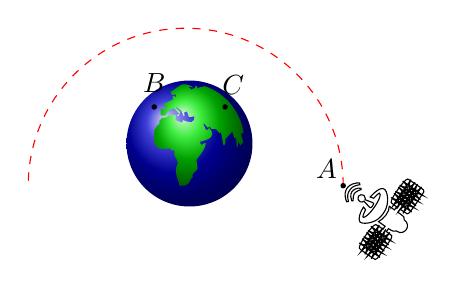
\begin{tikzpicture}
		\tikzset{earth/.pic={ 
		\shade[ball color=blue!80!black] (1.12,1.34) circle  (2);
		\shade[ball color=green!90!black] (1.6,3.16).. controls +(-18:0.68) and +(98:0.72).. 
			(2.84,1.66) --  (2.78,1.68).. controls +(-120:0.1) and +(90:0.1)..
			(2.82,1.38)..  controls +(-90:0.02) and +(90:0.02)..
			(2.74,1.28) -- (2.66,1.4) -- (2.66,1.24)  -- (2.62,1.24) -- (2.6,1.52) --
			(2.54,1.52) -- (2.48,1.72) -- (2.26,1.48) -- (2.26,1.32)  -- (2.2,1.28) --
			 (2.12,1.7) -- (2.08,1.66) -- (1.96,1.8) -- (1.82,1.8) -- (1.76,1.88) --
			(1.7,1.84) -- (1.58,1.98) -- (1.56,1.96) -- (1.64,1.78) -- (1.72,1.78)  --
			 (1.72,1.82) -- (1.76,1.82).. controls +(-50:0.4) and +(14:0.14)..
			(1.46,1.4).. controls +(-90:0.2) and +(180:0.08).. 
			(1.64,1.36).. controls +(-90:0.18)  and +(54:0.16)..
			(1.34,0.82) -- (1.38,0.56).. controls +(-79:0.06)  and +(63:0.08)..
			(1.22,0.36) -- (1.22,0.26) --  (1.16,0.22).. controls +(-96:0.1) and +(0:0.1)..
			 (0.94,0) -- (0.8,0).. controls +(90:0.16) and +(-120:0.3)..
			(0.74,0.68).. controls +(60:0.1)  and +(-90:0.02)..
			(0.64,0.96) -- (0.64,1.12) -- (0.56,1.12)..  controls +(104:0.04) and +(0:0.04)..
			(0.5,1.18)  -- (0.46,1.18).. controls +(190:0.4) and +(-90:0.1)..
			(0,1.42) --  (0,1.68).. controls +(90:0.1) and +(-146:0.08)..
			(0.16,1.96) -- (0.16,2.06) -- (0.26,2.16) -- (0.32,2.16).. controls +(0:0.12) and +(180:0.08).. 
			(0.5,2.24) -- (0.68,2.24) -- (0.68,2.08) -- (0.88,2) -- (0.92,2.08).. controls +(-16:0.08) and +(180:0.1).. 
			(1.14,2.02) -- (1.18,2.02).. controls +(0:0.08)  and +(-90:0.08)..
			(1.28,2.2) -- (1.1,2.18) -- (1.04,2.36) -- (0.94,2.32)..  controls +(-68:0.06) and +(0:0.04)..
			(0.94,2.2) -- (0.86,2.38) -- (0.7,2.5) -- (0.68,2.48) --  (0.82,2.34)..
			controls +(-117:0.06) and +(-53:0.12).. 
			(0.72,2.24) -- (0.8,2.28) --  (0.62,2.46) -- (0.52,2.42) -- (0.4,2.32)..
			controls +(-98:0.08) and +(-10:0.2).. (0.2,2.24)  -- (0.2,2.44) --
			(0.38,2.44) --  (0.32,2.58) -- (0.3,2.56) -- (0.3,2.6) -- (0.6,2.74)..
			controls +(90:0.04)  and +(-90:0.04)..
			(0.58,2.82).. controls +(0:0) and  +(0:0)..
			(0.62,2.86) -- (0.7,2.8) -- (0.68,2.9) -- (0.56,2.88)  --
			(0.52,2.98).. controls +(27:0.1) and  +(180:0.08)..
			(0.92,3.22) -- (0.98,3.22).. controls +(0:0.08) and +(124:0.04).. 
			(1.24,3.12)  -- (1.08,3.14) -- (1.2,3.04) -- (1.22,3.08) --
			(1.3,3.1) -- (1.3,3.16) -- (1.36,3.16) -- (1.36,3.1) -- cycle; 
			 }}
		\tikzset{vetinh/.pic={ 
		 \draw (5.76,24.88).. controls +(-160:0.3) and +(70:0.3)..
			(1.48,20.56).. controls +(-110:1)  and +(-165:1)..
			 (7.92,14.08).. controls +(22:0.4) and +(-135:0.8)..
			 (8.84,14.84) -- (9.56,15.56) -- (9.96,15.12) -- (10.4,14.72) -- (8.96,13.28).. controls +(-10:2) and +(110:2)..
			(13.2,9.04) -- (14.08,9.96)  -- (15,10.88) -- (15.8,10.04) -- (14.92,9.16).. controls +(-133:1.2) and +(63:0)..
			(13.96,8.04).. controls +(-110:1) and  +(-165:1)..
			 (20.44,1.6).. controls +(11:0.4) and +(-136:2.4)..
			(22.72,3.68).. controls  +(46:2.4) and +(-117:0)..
			(24.84,5.96)..  controls +(75:0.4) and +(-45:4.4)..
			(21.88,9.48).. controls  +(135:4.4) and +(15:0.4)..
			(18.36,12.44).. controls +(-166:0) and +(45:0.8).. 
			(17.44,11.68) -- (16.72,10.96)  -- (15.92,11.8)
			.. controls +(45:1.5) and  +(-60:0.5)..
			(17.08,14.1).. controls +(43:2)  and +(-45:0.65)..
			(17.16,17.36)..  controls +(135:1) and +(45:1.5)..
			(14,17.2).. controls  +(150:0.6) and +(45:1.5)..
			(11.96,16.28) -- (11.32,15.64) -- (10.48,16.48).. controls +(47:1.2) and  +(-104:0)..
			(12.32,18.48).. controls +(70:0.4) and  +(-45:4.4)..
			(9.44,21.96).. controls +(136:2.8) and  +(-18:0)..
			(6.4,24.88).. controls +(153:0.4) and +(27:0.4).. 
			(5.76,24.88)  --cycle;
		 \foreach \luc in {0,2.4,4.8,17.6,20,22.4}{
			\draw[rounded corners,shift={(-45:\luc)}] (7.2,21.96) -- (6.12,20.88)  -- (4.96,22) -- (6.08,23.08) --cycle
			[shift={(-135:2.5)}]  (7.2,21.96) -- (6.12,20.88) -- (4.96,22) -- (6.08,23.08) --cycle;
		} 
		\draw (3.12,12.32).. controls  +(-120:0.4) and +(106:0.4)..
			(3.16,10.96).. controls +(-71:0.8)  and +(126:1.2)..
			(4.72,8.2) --  (5,7.8) --(5.6,8.84).. controls +(90:0) and +(-90:0.4)..
			 (4.32,10.92).. controls +(90:0.4) and +(147:1.2)..
			(6.2,10.44).. controls +(-33:1.6)  and +(124:1.6)..
			(10.28,6.4)..  controls +(-56:1.2) and +(0:0.4)..
			(10.84,4.44).. controls +(180:0.4) and  +(0:0)..
			 (8.72,5.68) --
			(7.8,5.16).. controls +(-45:2) and  +(-150:1)..
			 (12.24,3.24).. controls +(25:1) and +(-50:3)..
			(11.72,10.04)..  controls +(125:0.8) and +(-38:0.8)..
			(10.04,11.76).. controls +(140:2.5) and  +(65:1.6).. cycle;
		\draw (6.92,8.32) -- 
			 (5.56,6.04).. controls +(0:0) and +(-45:0)..
			(5.48,6.08).. controls +(135:0) and  +(-18:0)..
			(5.16,6.2).. controls +(167:0.8) and +(90:0.8).. 
			(3.8,5.08).. controls +(-90:0.8) and  +(180:0.8)..
			(4.96,3.92)..  controls +(0:1) and +(-55:0.7)..
			(6,5.64)  --
			(8.28,7.12).. controls +(39:0.4) and  +(-45:0.4)..
			(7.96,8.08).. controls +(135:0.8) and +(54:0.4).. 
			(6.92,8.32)  --cycle;
		\draw (1.8,5.4).. controls +(-143:0.4)  and +(102:0.4)..
			(1.68,3.68).. controls +(-77:1.2) and +(174:1.2).. 
			 (3.88,1.76).. controls +(-6:0.4) and +(-162:0.4)..
			(5.16,1.84).. controls  +(27:0) and +(-53:0)..
			(5.28,2.28)..  controls +(170:0.5) and +(-40:0.5)..
			(3.28,2.88)..  controls +(160:0.5) and +(-85:1)..
			(2.2,5.4)..  controls +(162:0) and +(34:0)..
			 (1.8,5.4) --cycle;
		\draw (0.08,5.28).. controls  +(-119:0.4) and +(105:0.8)..
			(0,2.92).. controls +(-76:1.2)  and +(153:1.2)..
			(1.88,0.44).. controls +(-35:0.8) and  +(195:1)..
			(5.2,0.2) -- (5.23,0.75).. controls +(-174:0.4) and  +(-17:0.4)..
			(3.2,0.88).. controls +(163:0.8)  and +(-63:0.8)..
			 (1.04,2.68).. controls +(120:1) and +(-90:0)..
			(0.6,5.28)..  controls +(124:0) and +(63:0)..
			(0.08,5.28)  --cycle;
			 }}
		\path (0,0)  coordinate (O)
			(2,0) coordinate  (A)
			(-0.4,1) coordinate  (B)
			 (0.5,1) coordinate (C);
		 \draw[red,dashed] (2,0) arc (0:180:2cm);
		 \path (-0.4,0) pic[scale=0.4]{earth};
		\path (2,0) pic[scale=0.04,rotate=-80]{vetinh}; 
		\foreach \p/\r in {A/135,B/90,C/70} 
		\fill (\p) circle  (1pt) node[shift={(\r:3mm)}]{$\p$};
	\end{tikzpicture}
	} 
	 \shortans{-2,1}
	 \loigiai{
		Mặt cầu  $(S)$ có tâm $O(0; 0; 0)$, bán kính $R = \sqrt{3}$.\\
		Ta có $\heva{&\vec{AB} = (0; 4;  4)\\& vec{AC} = (2; 2; 4)} \Rightarrow[\vec{AB}, \vec{AC}] = (8; 8;-8) = 8(1; 1;-1) \Rightarrow (ABC) \colon x + y - z - 1 = 0$.\\
	\immini 
		{ Do $\mathrm{d}(O,(ABC)) = \dfrac{1}{\sqrt{3}}$ nên mặt phẳng  $(ABC)$ cắt mặt cầu $(S)$ theo giao tuyến là một đường tròn $(C)$ bán kính bằng
		$$r = \sqrt{R^2 - d^2} =  \dfrac{2\sqrt{6}}{3}.$$
		Chọn điểm $D$  thuộc $(C)$ sao cho $\triangle BCD$ đều, suy ra $D(1; 1; 1)$.
		 }
		{\begin{tikzpicture}[scale=1.2,font=\footnotesize,line join=round,line cap=round,>=stealth]
		\def\r{1.6} \def\h{0.6} \def\g{8} 
		\pgfmathsetmacro\a{sqrt ((\r)^2-(\h)^2)/cos (\g)} 
		\pgfmathsetmacro\b{\a/4} 
		 \pgfmathsetmacro\gm{asin (\h/\r)}
		\path (0,0) coordinate (O) 
			(-90:\h-.1)  coordinate (I)
			(-\gm:\r) coordinate (D) 
			(D) arc (-\g:\g-120:{\a}  and {\b}) coordinate (B)
			(D)  arc (-\g:\g+100:{\a} and {\b}) coordinate (C)
			(D) arc (-\g:\g+120:{\a} and {\b}) coordinate  (M)
			($(M)+(M)-(D)$) coordinate (A); 
		\draw (O)  circle (\r);
		\draw[dashed] (D) arc (-\g:180-\g:{\a} and {\b}) 
			(O)--(I)--(D)--(A) 
			 (B)--(C)--(D)--cycle;
		 \draw (D) arc (-\g:-180-\g:{\a} and {\b});
		 \foreach\x/\y in {O/90,I/-50,B/-70,D/-10,C/90,M/100,A/100}{
			\fill (\x)  node[shift={(\y:2mm)}]{$\x$} circle (0.05);
		} 
	\end{tikzpicture}
		}  \noindent
		 Xét điểm $M$ thuộc cung nhỏ $BC$, lấy $E$ thuộc đoạn $DM$ sao cho $MC = ME$ (1).\\
		Mặt khác $\widehat{CME} = \widehat{CBD} = 60^{\circ}$ (góc nội tiếp cùng chắn cung $CD$). Vì vậy  tam giác $CME$ đều.\\
		Xét hai $\triangle CMB$ và $\triangle CED$ có $\heva{&CM = CE, CB = CD \\& \widehat{CBM} = \widehat{CDE}.}$\\ 
		Do  đó $\triangle CMB = \triangle CED \Rightarrow MB = ED$ (2).\\
		Từ (1) và  (2) suy ra $MA + MB + MC = MA + ED + ME \geq AD = 2\sqrt{14}$.\\
		Dấu đằng thức xảy  ra khi $M = AD \cap (S)$ hay $M = AD \cap (C)$.\\
		Ta có phương trình tham số của đường thẳng $AD$ là $AD \colon  \heva{&x = 1 + t \\& y = 1 + 2t \\& z = 1 + 3t.}$\\
		Thay phương trình $AD$ vào phương trình $(S)$ thì 
		$$(1  + t)^2 + (1 + 2 t)^2 + (1 + 3t)^2 = 3 \Leftrightarrow \hoac{&t = 0 \\& t = -\dfrac{6}{7}.}$$
		\begin{itemize}
			\item Với $t =  0$ ta có điểm $D(1; 1; 1)$.
			\item Với $t = -\dfrac{6}{7}$ ta có điểm $M  \left(\dfrac{1}{7}; -\dfrac{5}{7}; -\dfrac{11}{7}\right)$.
		\end{itemize}
		 Suy ra $a + b + c = -\dfrac{15}{7} \approx -2{,}1$.
	 }
\end{bt}

% nguồn: Phan2_Lop_12_Hinh_hoc_Chuong_5
\begin{bt}%[2H5V3-4]%[ma:8f6ab1c0]
	Trong không gian với hệ toạ độ $Oxyz$, đài kiểm soát không lưu sân bay có toạ độ $O(0; 0; 0)$, mỗi đơn vị trên trục ứng với 1 km. Máy bay bay trong phạm vi cách đài kiểm soát 417 km sẽ hiển thị trên  màn hình ra đa. Một máy bay đang ở vị trí $A(-688;-185; 8)$, chuyển động theo đường thẳng $d$ có vectơ chỉ phương là $\vec{u}=(91; 75; 0)$ và hướng về đài kiểm soát không lưu.
	\begin{center}
		\begin{tikzpicture}[line join = round,line cap=round,>=stealth,font=\footnotesize,scale=1]
				\def  \daiE{2}
				 \path
					(0,0) coordinate (X1) 
					 --(7,0) coordinate (X2)
					--(9,5) coordinate  (X3)
					--($(X1)+(X3)-(X2)$) coordinate  (X4)
					--cycle 
					($(X2)!1/2!(X4)$) coordinate (tamE) 
					 ($(tamE)-(\daiE,0)$) coordinate (Etrai)
					($(tamE)+(\daiE,0)$) coordinate  (Ephai)
					($(tamE)+(160:2)$) coordinate  (B)
					($(tamE)+(10:2)$) coordinate  (C);
				\draw[fill=cyan,opacity=0.2] (X1)--(X2)--  (X3)--(X4)--cycle;
				\draw[dashed] (tamE) ellipse (\daiE  cm and 1cm)
					 (B)--(C);
				\draw (Ephai) arc (0:-180:\daiE cm  and 1cm);
				\draw[->,dashed] ($(Etrai)!-0.2!(Ephai)$)--($(Etrai)!1.2!(Ephai)$) node[below]{$y$}; 
				\draw[->,dashed] ($(tamE)+(1.5,1.5)$)--($(tamE)+(-1.5,-1.5)$) node[below]{$x$}; 
				\draw[->,dashed] ($(tamE)+(0,-2)$)--($(tamE)+(0,3)$)  node[above]{$z$};
				\draw[fill=red,opacity=0.4] (tamE)  circle (2cm);
				\draw[fill=brown,opacity=0.2] (Ephai) arc (0:-180:\daiE cm and 1cm)--(Etrai) arc (180:360:2cm  and 2cm);
				\draw 
					(tamE)  circle (1pt) node[below right]{$O$}
					(B) circle  (1pt) node[above right]{$B$}
					(C) circle (1pt)  node[above right]{$C$}
					(B)--($(B)!-0.2!(C)$)  node[above]{$A$}
					(C)--($(B)!1.2!(C)$)  node[above]{$d$};
			\end{tikzpicture}
	\end{center}
	Tính  khoảng cách ngắn nhất giữa máy bay và đài kiểm soát không lưu. Kêt quả làm tròn đến hàng đorn vị. \\
	 \shortans{295}
	\loigiai{ 
		Phương trình tham số của đường thẳng $d$ là: $\left\{\begin{array}{l}x=-688+91 t \\ y=-185+75 t \\ z=8
	\end{array}\right.$\\
	Gọi $H$ là vị trí mà máy  bay bay gần đài kiểm soát không lưu nhất.\\
	Khi đó, khoảng OH là ngắn nhất giữa máy bay và đài kiểm soát không lưu, điều này xảy ra khi và chỉ khi  $O H \perp d$.\\
	Vì  $H \in d$ nên $H(-688+91 t;-185+75 t; 8)$.\\
	Ta có $\overrightarrow{\mathrm{OH}}=(-688+91 t;-185+75  t; 8)$.\\
	 Do đó
	$O H \perp d \Leftrightarrow \overrightarrow{O H} \perp \vec{u} \Leftrightarrow \overrightarrow{O H} \cdot \vec{u}=0\\ \Leftrightarrow(-688+91 t) \cdot 91+(-185+75 t) \cdot 75=0 \Leftrightarrow t=\dfrac{11}{2}$.\\ 
	Suy ra  $H\left(-\dfrac{375}{2}; \dfrac{455}{2}; 8\right)$.\\
	Khoảng cách ngắn  nhất giữa máy bay và đài kiểm soát không lưu là
	 $$
	O H=\sqrt{\left(-\dfrac{375}{2}\right)^2+\left(\dfrac{455}{2}\right)^2+8^2}  \approx 295 \mathrm{~km}.
	 $$
	 }
	\end{bt}

% nguồn: Phan2_Lop_12_Hinh_hoc_Chuong_5
\begin{bt}%[2H5V3-4]%[ma:d5f3feae]
	Một nguồn âm phát ra sóng âm là sóng cầu (mặt đầu sóng là mặt cầu). Khi gắn hệ trục tọa độ $Oxyz$ với đơn vị trên mỗi trục là mét, vị trí nguồn âm có tọa độ $(0;-3;-1)$, cường độ âm chuẩn phát ra có bán kính là $10$ mét. Một bạn học sinh di chuyển theo phương thẳng từ vị trí $N(7;10;-4)$ đến vị trí $M(5;0;2)$ để nhận nguồn âm. Khi bạn học sinh đó di chuyển từ $N$ đến $M$ thì vị trí  đầu tiên nhận được nguồn âm là $A\left(x_0;y_0;z_0\right)$. Tính tổng $x_0+y_0+z_0$.
	\begin{center}
		\begin{tikzpicture}[scale=.5]
				 \tikzset{Athlete/.pic={
				\fill (-0.35,2.2)..controls++(-85:0.35) and++(90:0.2)..(-0.1,1.5)..controls++(-90:0.2) and++(50:0.15)..(-0.2,1.2)..controls++(-140:0.5) and++(98:0.25)..(-0.45,0.35)..controls++(-120:0.25) and++(80:0.5)..(-0.8,-0.6)..controls++(-110:0.25) and++(70:0.35)..(-1.3,-1.3)..controls++(-110:0.35) and++(-30:0.25)..(-2.1,-2.05)..controls++(160:0.25)  and++(90:0.25)..(-2.25,-2.7)..controls++(-90:0.3) and++(-70:0.55)..(-2,-2.8)..controls++(110:0.02) and++(-110:0.35)..(-1.78,-2.25)..controls++(32:0.8) and++(-142:1)..(-0.35,-1.15)..controls++(38:0.1) and++(-100:0.5)..(0.2,0)..controls++(-25:0.25) and++(175:0.5)..(1.35,-0.15)..controls++(-140:0.35) and++(40:0.35)..(0.6,-1)..controls++(-160:0.5) and++(112:0.75)..(0.5,-1.75)..controls++(-68:0.1) and++(-68:0.65)..(0.75,-1.8)..controls++(88:0.5) and++(-155:0.25)..(1,-1.08)..controls++(25:0.25) and++(-165:0.25)..(2.2,-0.15)..controls++(15:0.05) and++(-90:0.05)..(2.25,0)..controls++(90:0.35) and++(5:0.15)..(0.6,0.75)..controls++(90:0.15) and++(-85:0.1)..(0.85,1.6)..controls++(-50:0.7) and++(-140:1)..(1.95,2.2)..controls++(40:0.01) and++(-88:0.25)..(1.95,2.4)--++(155:0.28)--++(-132:0.25)..controls++(-82:0.45) and++(50:0.25)..(1.15,1.75)..controls++(110:1) and++(-10:0.05)..(0.65,2.68)..controls++(75:0.3) and++(-60:0.25)..(0.9,2.95)..controls++(30:0.02) and++(-30:0.085)..(0.92,3)--++(20:0.05)--++(95:0.08)--++(40:0.1)..controls++(90:0.05) and++(-100:0.25)..(0.95,3.45)..controls++(100:0.75) and++(135:0.75)..(.2,3.1)--++(-88:0.2)..controls++(-158:0.25) and++(30:1)..(-1.3,2.26)..controls++(-105:0.5) and++(100:0.5)..(-1.35,1)..controls++(-108:0.15) and++(150:0.3)..(-1.4,0.5)--++(-5:0.25)--++(70:0.25)--++(110:0.2)..controls++(110:0.15) and++(-100:1)..(-0.9,2)..controls++(20:0.1) and++(-110:0.15)..(-0.35,2.2);
					 }}
				\draw (25,0) coordinate (N) pic[orange, 
					 scale=0.4]{Athlete};
				 \draw (0,1)--(0,-1)--(1,-1)--(3,-3)--(3,3)--(1,1)--(0,1)--cycle;
				\draw  [line width=12](3.2,2.725) arc (90:-90:2.7);
				\draw [line width=12](3.2,1.725) arc  (90:-90:1.7);
				 \draw [line width=12](3.2,0.725) arc (90:-90:.7);
				\coordinate  (H) at (18,3);
				 \coordinate (G) at (7,0);
				\coordinate  (I) at (18,-3);
				\foreach \diem in {20,40,...,200} \draw pic[draw,angle radius=\diem]{angle=I--G--H}; 
				\coordinate  [label=below:$M$](M) at (8,-6);
				 \coordinate [label=below:$N$](N) at (25,-4);
				\draw[dashed](N)--($(N)!  1.5 ! (M)$);
				\foreach \diem in {M,N} \fill (\diem) circle  (4pt);
			\end{tikzpicture}
	\end{center}
	 \shortans{10}
	 \loigiai{
		Phương trình mặt  cầu mô tả sóng âm phát ra từ nguồn âm là
		$$(S)\colon x^2+(y+3)^2+(z+1)^2=100.$$ 
		Ta  có $\overrightarrow{N M}=(-2;-10; 6)\Leftrightarrow MN\colon \heva{&x=7-t \\& y=10-5 t \\& z=-4+3 t}$, $t \in \mathbb{R}$.\\
		Tọa độ giao điểm của  mặt cầu ( $S$) và đường thẳng $MN$ là nghiệm của hệ
		\allowdisplaybreaks 
		\begin{eqnarray*}
			\heva{&x=7-t \\& y=10-5 t \\& z=-4+3 t \\& x^2+(y+3)^2+(z+1)^2=100}&\Rightarrow&(7-t)^2+(13-5 t)^2+(-3+3 t)^2=100\\&\Leftrightarrow& 35 t^2-162 t+127=0  \Leftrightarrow\hoac{&t=1 \\& t=\dfrac{127}{35}} \\&\Rightarrow&\hoac{&A_1(6;5;-1)\\&A_2\left(\dfrac{118}{35};-\dfrac{57}{7};\dfrac{241}{35}\right)}
		\end{eqnarray*}
		Các giao điểm là $A_1(6;  5;-1);A_2\left(\dfrac{118}{35};-\dfrac{57}{7}; \dfrac{241}{35}\right)$. Khi đó
		 \allowdisplaybreaks
		\begin{eqnarray*}
			NA_1&=&\sqrt{1^2+5^2+(-3)^2}=\sqrt{35};\\NA_2&=&\sqrt{\left(\dfrac{118}{35}-7\right)^2+\left(-\dfrac{57}{7}-10\right)^2+\left(\dfrac{241}{35}+4\right)^2} \approx  21{,}5.
		\end{eqnarray*}
		Ta có $NA_1<N A_2$ nên $A_1(6; 5;-1)$ là vị trí đầu tiên nhận  được nguồn âm. Khi đó $x_0+y_0+z_0=10$.
	} 
\end{bt}

% nguồn: Phan2_Lop_12_Hinh_hoc_Chuong_5
\begin{bt}%[2H5V3-4]%[ma:620bf78e]
	Trong không gian $Oxyz$ (đơn vị của các trục tọa độ là kilômét), một trạm thu phát sóng điện thoại di động có đầu thu phát được đặt tại điểm $I\left(-2;1;-4\right)$. Biết bán kính phủ sóng của trạm là  $3$ km. Có $5$ người sử dụng điện thoại tại các điểm $A\left(2;-1;3\right)$, $B\left(0;1;-4\right)$, $C\left(-2;1;-3\right)$, $ D\left(0;1;-3\right)$, $ E\left(-4;-2;1\right)$. Hỏi trong số $5$ người đó, có bao nhiêu người có thể sử dụng được dịch vụ của trạm nói trên?
	\shortans{3} 
	\loigiai{ 
		Ta tính $IA=\sqrt{4^2+\left(-2\right)^2+7^2}=\sqrt{69}>3$; $IB=\sqrt{2^2+0^2+0^2}=2<3$.\\ 
		$IC=\sqrt{0^2+0^2+1^1}=1<3$;  $ID=\sqrt{2^2+0^2+1^2}=\sqrt{5}<3$; $IE=\sqrt{\left(-2\right)^2+\left(-3\right)^2+5^2}=\sqrt{38}>3$.\\
		Vậy có $3$  người có thể sử dụng dịch vụ của trạm nói trên.
	 }
\end{bt}

% nguồn: Phan2_Lop_12_Hinh_hoc_Chuong_5
\begin{bt}%[2H5V3-4]%[ma:1d5350a9]
	 \immini{
	Một quả bóng hình cầu có bán kính $r$ đang được treo trong một góc của tường nhà (hai bờ tường vuông góc với nhau). Một điểm $B$ cố định nằm trên mép hai bờ  tường và cách mặt đất $80$\,cm, sợi dây treo quả bóng có độ dài $AB=30$\,cm và đây cũng là độ dài ngắn nhất nối điểm $B$ với mặt xung quanh của quả bóng. Biết rằng quả bóng tiếp xúc với hai bên bờ tường và điểm thấp nhất của quả bóng cách mặt đất $20$\,cm. Hỏi quả bóng có đường kính là bao nhiêu cm (làm tròn kết quả đến hàng đơn vị)?
	 }
	{ 
	\begin{tikzpicture}[scale=1,>=stealth,line join=round,line cap=round,font=\footnotesize]
			\def\g{-10} 
			\def\r{.96} 
			 \pgfmathsetmacro\ra{sqrt (1-(\r)^2)}
			\pgfmathsetmacro\a{cos  (\g)}
			\pgfmathsetmacro\b{sin (\g)} 
			\pgfmathsetmacro\ax{\ra*cos  (\g)/sqrt ((\ra*\a)^2+(\b)^2)}
			 \pgfmathsetmacro\bx{\ra*sin (\g)/sqrt ((\ra*\a)^2+(\b)^2)}
			\path 
				 (0,0) coordinate (O)
				+({\ax},{\bx}) coordinate  (i)
				+({\bx/\ra},{-\ax*\ra}) coordinate  (j)
				+(0,{\r})  coordinate (k)
				+($(i)+(j)+1.5*(k)$)  coordinate (bas) coordinate (I)
				($(bas)+\r*0.74*(k)$) coordinate (A) 
				($3.2*(k)$)  coordinate (B);
			 \fill [orange!60!black!40] ($3*(i)$)--(O)--($3*(j)$)--cycle;
			\fill [cyan!60!black!60] (O)--($3.5*(k)$)--($3*(j)+3.5*(k)$)--($3*(j)$)--cycle; 
			\fill [gray!10] (O)--++($.1*(k)$)--++($3*(j)$)--++($-.1*(k)$)--cycle; 
			 \fill [cyan!60!black!40] (O)--($3.5*(k)$)--($3*(i)+3.5*(k)$)--($3*(i)$)--cycle;
			\fill  [gray!10] (O)--++($3*(i)$)--++($.1*(k)$)--++($-3*(i)$)--cycle;
			\draw[dashed,->|] (bas)--++($-1.55*(k)$) node[pos=0.65,right]{\scriptsize $20$\,cm}; 
			 \draw[->](O)--($3.5*(i)$) node[below]{$y$};
			 \draw[->](O)--($3.5*(j)$) node[below]{$x$};
			\draw[->](O)--($4*(k)$)  node[left]{$z$};
			\begin{scope}[scale=.15]
				\path (bas)++(-90:4.54) coordinate (N); 
				\fill [ball color= orange!100!brown,opacity=0.4] (bas) circle (4.54); 
				 \draw (bas)++(1.95,4.1).. controls +(-4.92,.71) and +(-3.58,2.6).. ++(-3.83,-8.24)
					(bas)++(-4.38,1.2).. controls +(1.46,-2.07) and +(-2.73,-.4).. ++(8.34,-3.42) 
					(bas)++(-3.44,2.97).. controls +(-.2,-3.87)  and +(-3.45,3.16).. ++(7.96,-2.55)
					(bas)++(-4.52,-.48)..  controls +(2.12,.59) and +(-4.79,.72).. ++(5.92,-3.83);
			\end{scope}
			\draw[red] (B)--(A) node[pos=0.5,right]{\scriptsize  $30$\,cm}
				 (I)--++(0.72*\r,0) node[pos=0.5,below=-0.65mm]{\footnotesize $r$};
			 \foreach \x /\gN in {A/30,B/0,I/180,O/160}
			 \fill (\x) circle (1pt)
				 ($(\x)+(\gN:2mm)$) node {$\x$};
		\end{tikzpicture}
	} 
	\shortans{38} 
	 \loigiai{
		Gọi tâm quả bóng là $I(a;b;c)$ bán kính $r$.\\ Dựa vào hình vẽ ta có $a;b;c  > 0$ và điểm $B(0;0;80)$. \\
		Ta có $AB\ge |IB-IA|=IB-r$.\\ Do đó $IB-r=30\Leftrightarrow\sqrt{a^2+b^2+(c-80)^2}=r+30$.\quad $(1)$ \\ 
		Quả bóng tiếp xúc với  hai bên bờ tường nên $\mathrm{d}(I,(Oxz))=\mathrm{d}(I,(Oyz))=r\Leftrightarrow b=a=r$.\quad $(2)$ \\
		Điểm thấp nhất của quả bóng cách  mặt đất $20$\,cm nên $\mathrm{d}(I,(Oxy))=r+20\Leftrightarrow c=r+20$.\quad $(3)$ \\
		Vì dây treo  quả bóng nên điểm $I$ phải thấp hơn điểm $B$ nên $c < 80$ hay $r+20< 80\Rightarrow r < 60$. \\
		Thế $(2)$, $(3)$ vào $(1)$ ta có 
		\begin{eqnarray*}
			&&\sqrt{r^2+r^2+(r+20-80)^2}=r+30\\ 
			&\Leftrightarrow&  3r^2-120r+3600=r^2+60r+900\\
			 &\Leftrightarrow&2r^2-180r+2700=0\\
			&\Leftrightarrow&\hoac{&r=45+15\sqrt{3}\\&r=45-15\sqrt{3}.} 
		\end{eqnarray*}
		Đối chiếu $r  < 60$ ta có $r=45-15\sqrt{3}$.\\
		Vậy đường kính quả cầu là  $r=90-30\sqrt{3}\approx 38$\,cm.
	 }
\end{bt}

% nguồn: Phan2_Lop_12_Hinh_hoc_Chuong_5
\begin{bt}%[2H5V3-4]%[ma:171ea7a1]
	 \immini{
	Trong không gian hệ trục tọa độ $Oxyz$, đài kiểm soát không lưu sân bay có tọa độ $O(0;0;0)$, mỗi đơn vị trên trục ứng với $1$ km. Máy bay trong phạm vi cách đài kiểm soát $417$ km sẽ hiển thị trên màn hình ra đa. Một  máy bay đang ờ vị trí $A(222;565;8)$ chuyển động theo đường thẳng $d$ có vectơ chỉ phương $\vec{u}(91;75;0)$ và hướng về đài kiểm soát không lưu (như hình vẽ). Tọa độ của vị trí sớm nhất mà máy bay xuất hiện trên màn hình ra đa là $M(a;b;c)$. Khi đó $a+b+c$ bằng bao nhiêu?
	} 
	 {
	\begin{tikzpicture}[scale=1,font=\footnotesize,line join=round,
				line  cap=round,>=stealth]
			 \draw (-4.5,0)--(-2,0)
				(0,-3)--(0,-2); 
			\draw[->] (2,0) --(4,0) node[below]{$y$}; 
			\draw[->] (0,2) --(0,3)  node[left]{$z$};
			 \draw[dashed] (-2,0)--(0,0) coordinate (O) --(2,0)
				 (0,-2)--(0,2);
			\draw[dashed] (O)--++(55:1.5) 
				(O)--++(-125:1.25)  coordinate (I);
			 \draw[->] (I)--++(-125:1.5) node[right]{$x$};
			\draw[dashed,name path=a]  (-2,0) arc (180:0:2);
			\draw (-2,0)  arc (-180:180:2);
			\draw[dashed,name  path=e] (-2,0) arc (180:0:{2} and {1});
			\draw  (-2,0) arc (-180:0:{2} and {1});
			\path[name  path=t] (-4,.9) coordinate (A)--(3,.3) coordinate (d);
			\path[name  intersections={of=e
				and  t}]
				 (intersection-1) coordinate (B)
				 (intersection-2) coordinate (C);
			\path[name intersections={of=a 
				and  t}]
				(intersection-1)  coordinate (X)
				(intersection-2)  coordinate (Y);
			 \draw (A)--(X)
				 (Y)--(d);
			\draw[dashed]  (X)--(Y);
			 \foreach \x/\g in {A/180,B/-90,C/-140,d/90,O/-45}
			 \fill (\x) circle (1pt)
				($(\x)+(\g:3mm)$) node{$\x$}; 
		\end{tikzpicture}
	} 
	\shortans{463} 
	 \loigiai{
		Vùng phủ sóng Rada được phát ra từ trạm kiểm soát là tập hợp những điểm cách tâm $O(0;0;0)$ không quá $417$ km. Đây là những điểm nằm  trên bề mặt và bên trong khối cầu có phương trình
		$$x^2+y^2+z^2=417^2 \Leftrightarrow x^2+y^2+z^2=173\,889.\quad  (*)$$
		Quỹ đạo chuyển động của máy bay là một đường thẳng có phương trình  $$d\colon \heva{&x=222-91t\\& y=565-75 t\\& z=8} (t \in \mathbb{R}).$$
		Máy bay bắt đầu thuộc vùng kiểm soát  của ra đa khi $M(222-91t;565-75t;8)$ thỏa mãn $(*)$.
		Suy ra $(222-91 t)^2+(565-75 t)^2+8^2=173\,889 \Leftrightarrow 13\,906  t^2-125\,154 t+194\,684=0 \Leftrightarrow\heva{&t=2 \\&t=7.}$\\
		Với $t=2$, ta  có $M(40;415;8) \Rightarrow AM^2=55\,624$. \\
		Với $t=7$, ta có  $M(-415;40;8) \Rightarrow A M^2=681\,395$.\\
		Vậy $M(40;415;8) \Rightarrow  a+b+c=463$.
	 }
\end{bt}

% nguồn: Phan2_Lop_12_Hinh_hoc_Chuong_5
\begin{bt}%[2H5V3-4]%[ma:1b59aa41]
	\immini{Trong một tiết thực hành về quan sát quả địa cầu có một nhóm học sinh cầm một quả địa cầu sao cho nó không chạm vào mặt bàn. Trên mặt bàn có một tờ giấy hình tam giác $ABC$. Xét trong không gian $Oxyz$, tam giác $ABC$ có $A(3;0;0)$, $B(0;5;0)$, $C(0;5;1)$. Giả sử bề mặt quả địa cầu là mặt cầu $(S)\colon x^2+y^2+(z-3)^2=\dfrac{49}{20}$. Cô giáo khẳng định trên quả địa cầu $(S)$ tồn tại duy nhất một điểm $M(a;b;c)$ sao cho biểu thức $T=MA^2+MB^2+MC^2$ đạt giá trị lớn nhất và yêu cầu nhóm học sinh đó đi tìm điểm $M$ nêu trên. Tổng $a+b+c$ bằng bao nhiêu (\textit{làm tròn kết quả đến hàng phần trăm})?}{\begin{tikzpicture}[line join=round,line cap=round,scale=.8,transform shape]
		 \definecolor{ao (english)}{rgb}{0.0,0.5,0.0}
		 \definecolor{ceruleanblue}{rgb}{0.16,0.32,0.75}
		\definecolor{brown  (traditional)}{rgb}{0.59,0.29,0.0}
		 \tikzset{earth/.pic={
		\def\D{ 
			(0,0)  circle (4.9cm);
		} 
		 \fill[ball color=ceruleanblue] \D;
		 \draw\D;
		\def\N{ 
			(-.2,4.87) 
			..controls  +(180:1.52) and +(60:1.5)..(-4.16,2.55)
			..controls +(-80:.5) and +(160:.5)..(-3.7,1.75) --(-3.8,1.55) 
			..controls  +(-45:.5) and +(130:.5)..(-3.45,1)
			..controls +(-20:1)  and +(135:1.9)..(-3.1,-1)
			..controls +(-100:.5) and +(85:.9)..(-3,-2) 
			..controls  +(-95:.5) and +(85:.7)..(-3.1,-3)
			..controls  +(-75:.5) and +(155:.7)..(-2.4,-4.25) --(-2.5,-3.45)
			..controls +(65:1) and +(-125:1.5)..(-1.4,-2.1) 
			..controls +(15:1) and +(-140:1)..(-.3,-.8) 
			..controls +(40:.4) and +(-85:.6)..(-1.3,.3) 
			..controls +(95:.4)  and +(-45:.6)..(-2.6,1.2)
			..controls +(145:.4)  and +(-75:1.2)..(-3.5,1.5)
			..controls +(55:.4) and +(-135:.5)..(-3.4,1.9) 
			..controls +(45:.2)  and +(-35:.2)..(-3.65,2.1)
			..controls +(145:.6) and  +(105:1)..(-2.65,2.4)
			..controls  +(-75:.5) and +(-105:.6)..(-2.45,2.9)
			..controls +(45:.5) and  +(-145:.6)..(-1.5,3.3)
			..controls  +(35:.5) and +(-145:.6)..(-.8,3.5)
			..controls  +(35:.2) and +(-100:.7)..(-.3,3.8)
			..controls  +(-150:.2) and +(-130:.2)..(-.3,4.1)
			 ..controls +(140:.7) and +(-30:.3)..(-1,4.15)
			..controls  +(-130:.7) and +(-160:.5)..(-1.1,4.4)--(-1,4.45)--(-.9,4.4)
			 ..controls +(30:.3) and +(140:.3)..(-.35,4.3)--(0,4.6)--cycle;
		} 
		\draw\N; 
		 \fill[ao (english)] \N;
		 \def\N{
			(2.65,4.1) 
			..controls +(-30:3.4)  and +(32:3.3)..(2.8,-4)
			..controls +(-148:.4) and +(-120:.3)..(2.95,-3.1) 
			..controls +(120:.4)  and +(-120:.5)..(3.3,-2)
			..controls +(120:.4)  and +(-90:.6)..(3.3,-.8)
			..controls +(100:.2) and  +(20:.1)..(3.1,-.8)
			..controls +(120:1) and +(-50:2)..(1.5,0) 
			 ..controls +(80:1) and +(-150:.6)..(2,1.5)
			..controls +(30:.6) and  +(170:.8)..(3.2,1.9)
			..controls  +(-10:.6) and +(180:.8)..(4.5,1.45)
			..controls +(120:.6) and  +(-50:.9)..(3.9,2.1)
			 ..controls +(-120:.2) and +(-50:.2)..(3.6,2.2)
			..controls +(-120:.2) and  +(-100:.2)..(3.4,2.3)
			 ..controls +(150:.4) and +(85:.4)..(2.9,2.1)
			..controls +(-160:.6) and  +(-55:.6)..(2.1,2.5)
			..controls +(30:.6)  and +(-140:.6)..(2.9,2.9)
			 ..controls +(120:.3) and +(-100:.3)..(2.9,3.3)--(2.65,3.33)--(2.5,3.5)
			..controls +(180:.3) and +(-90:.3)..(2.2,4)--cycle; 
		} 
		\draw\N; 
		\fill[ao (english)] \N; 
		\def\N{ 
			 (0,4.9)
			..controls +(0:.2) and +(165:.2)..(1.1,4.78)--(.95,4.35) 
			..controls +(-165:.7) and  +(45:.6)..(.25,3.85)
			..controls +(155:.7)  and +(-45:.6)..cycle
			(.7,4) 
			 ..controls +(155:.2) and +(-145:.2)..(1,4.2)
			..controls +(-45:.2) and  +(90:.2)..(1,3.9)
			..controls +(155:.2)  and +(-25:.2)..cycle
			 (2.2,3.5)
			..controls  +(-30:.2) and +(125:.2)..(2.55,3.05)
			..controls +(-150:.2) and  +(-80:.5)..(2.15,3.25)--(2,3.15)--(1.9,3.25)--(2.1,3.45)
			..controls +(130:.2) and  +(100:.2)..cycle
			 (-3,2)
			..controls  +(40:.2) and +(165:.8)..(-2.2,2)
			..controls +(-40:.2) and  +(-165:.8)..cycle
			(-2.5,1.6) 
			..controls +(40:.2) and  +(140:.2)..(-2,1.7)
			..controls +(-40:.2) and +(-140:.2)..cycle; 
		} 
		\draw\N; 
		\fill[ao (english)] \N; 
			 }}
		 \path
			 (0,0) pic[scale=.4]{earth};
		\coordinate (A) at  (-3,-2.5);
		\coordinate (B) at  (-6,-5);
		\coordinate (C) at  (1,-5);
		 \coordinate (D) at ($(C)-(B)+(A)$);
		 \coordinate (E) at (0,-3);
		\coordinate  (F) at (-3,-4);
		\coordinate (G) at (1,-4); 
		 \draw[smooth](B)--(C)--(D)--(A)--(B)
			 (E)--(F)--(G)--(E);
	\end{tikzpicture}
	} 
	 \shortans{2,40}
	\loigiai{ 
		\begin{itemize}
			\item Gọi $G$ là trọng tâm tam  giác $ABC$ ta có $G\left(1;\dfrac{10}{3};\dfrac{1}{3}\right)$ Khi đó
			$$T=MA^2+MB^2+MC^2=GA^2+GB^2+GC^2+3MG^2.$$ Do đó biểu thức $T=M A^2+M B^2+M C^2$ đạt giá trị lớn nhất khi và  chỉ khi $G M$ lớn nhất.
			\item Ta có $\overrightarrow{IG}=\dfrac{1}{3}(3;10;-8)$ trong đó  $I(0;0;3)$ là tâm mặt cầu $(S)$. \\Khi đó đường thẳng $I G\colon \heva{&x=3t\\&y=10t\\&z=3-8t.}$
			\item Thay $x=3t;y=10t;z=3-8t$ vào phương trình mặt cầu ta có $t= \pm \dfrac{7}{\sqrt{3460}}$. \\Hay đường  thẳng $IG$ cắt mặt cầu $(S)$ tại hai điểm $$M_1\left(\dfrac{21}{\sqrt{3460}};\dfrac{70}{\sqrt{3460}};3-\dfrac{56}{\sqrt{3460}}\right), M_2\left(-\dfrac{21}{\sqrt{3460}};-\dfrac{70}{\sqrt{3460}};3+\dfrac{56}{\sqrt{3460}}\right).$$
			\item Dễ thấy $\overrightarrow{IG}$; $\overrightarrow{IM_1}$ cùng hướng nên  $G M$ lớn nhất khi $M \equiv M_2$ hay $$M\left(-\dfrac{21}{\sqrt{3460}};-\dfrac{70}{\sqrt{3460}};3+\dfrac{56}{\sqrt{3460}}\right).$$
		\end{itemize}
		Khi đó $a+b+c=\dfrac{-21-70+56}{\sqrt{3460}}+3 \approx 2{,}40$. 
	} 
\end{bt}

% nguồn: Phan2_Lop_12_Hinh_hoc_Chuong_5
\begin{bt}%[2H5V3-4]%[ma:8537666c]
	\immini{ 
	Một cơ sở sản xuất Kem làm một mô hình Kem ốc quế lớn gồm $2$ phần: Phần Kem có dạng hình cầu, phần ốc quế có dạng hình nón (như hình vẽ bên). Chủ cơ sở  sản xuất muốn gắn một chiếc đèn Led lớn chiếu thẳng cây kem vào buổi tối, biết rằng chiếc đèn nằm trên mặt phẳng chứa đường tròn $(C)$ là phần tiếp xúc giữa phần Kem và phần ốc quế. Chọn hệ trục tọa độ $Oxyz$ trong không gian thỏa mãn
	phần Kem hình cầu  có tâm $I(1;2;3)$, bán kính $R_C=3$ và phần đỉnh của hình nón là điểm $H(0;1;-2)$ đáy là đường tròn có bán kính $R_N=\sqrt{6}$. Để tối ưu hóa lượng ánh sáng chiếc đèn có thể chiếu vào cây kem người ta tính toán rằng chiếc đèn Led sẽ phải ở vị trí $M(a;b;2), a \in \mathbb{Z}$ và từ điểm $M$ kẻ được $2$ tiếp tuyến với đường tròn $(C)$ sao cho góc giữa $2$ tiếp tuyến đó không bé hơn $60^{\circ}$. Có bao nhiêu vị trí đặt chiếc đèn Led thỏa mãn yêu cầu của chủ cơ sở.}
	{	\begin{tikzpicture}[scale=0.7,font=\footnotesize,line join=round,
			line cap=round,>=stealth] 
		\draw  (0,0) coordinate (O) arc (210:-30:3);
		\draw[dashed] (0,0) coordinate  (O) arc (-150:-30:3);
		 \draw[dashed] (O) arc (180:65:{2.6} and {.5}) coordinate (C) arc (65:0:{2.6} and {.5}) coordinate (J);
		\draw (O) arc (-180:-50:{2.6} and  {.5}) coordinate (D) arc (-50:0:{2.6} and {.5});
		\draw[dashed] (2.6,0)  coordinate (A) --++(90:1.5) coordinate (I)
			(A)--++(-90:5)  coordinate (H);
		\draw  (H)--(O)
			(H)--(J); 
		\foreach \x/\g in  {I/0,H/-90}
		\fill (\x) circle (1pt) 
			($(\x)+(\g:3mm)$)  node{$\x$};
	\end{tikzpicture}
	} 
	 \shortans{6}
	 \loigiai{
		\begin{center}
			\begin{tikzpicture}[scale=0.7,font=\footnotesize,line join=round,
						line cap=round,>=stealth] 
					\draw (0,0) coordinate  (O) arc (210:-30:3);
					\draw[dashed] (0,0) coordinate (O)  arc (-150:-30:3);
					\draw[dashed] (O) arc  (180:65:{2.6} and {.5}) coordinate (C) arc (65:0:{2.6} and {.5}) coordinate (J);
					\draw (O) arc (-180:-50:{2.6} and {.5}) coordinate  (D) arc (-50:0:{2.6} and {.5});
					\draw[dashed] (2.6,0) coordinate (A) --++(90:1.5) coordinate  (I)
						(A)--++(-90:5)  coordinate (H);
					\draw[dashed] (C)--++(-3:1.8)  coordinate (M');
					\draw  (M')--++(-3:4) coordinate (M);
					\draw  ($(M)!.6!(A)$)--(M);
					\draw[dashed] ($(M)!.6!(A)$)--(A)--(C) 
						 (A)--(D);
					\draw (M)--(D); 
					\draw  (H)--(O)
						 (H)--(J);
					\foreach  \x/\g in {A/180,I/0,C/90,D/-110,H/-90,M/0}
					\fill (\x)  circle (1pt)
						($(\x)+(\g:3mm)$) node{$\x$}; 
				\end{tikzpicture}
		\end{center}
		Gọi $A$ là tâm của  đường tròn $(C)$ và $MC$, $MD$ là hai tiếp tuyến kẻ từ $M$ đến $(C)$.\\
		Ta  có $\overrightarrow{IH}=(-1;-1;-5)$, suy ra $IH=\sqrt{(-1)^2+(-1)^2+(-5)^2}=3\sqrt{3}$, $IA=\sqrt{R_C^2-R_N^2}=\sqrt{3^2-6}=\sqrt{3}$.
		Vì $\overrightarrow{IH}=3\overrightarrow{IA}$ nên $\heva{& 0-1=3(x_A-1)\\&1-2=3(y_A-2)\\&-2-3=3(z_A-3)}\Rightarrow \heva{&x=\dfrac{2}{3} \\&y=\dfrac{5}{3} \\&z=\dfrac{4}{3}.}$\\ 
		Vậy hình nón có đáy  là đường tròn có tâm $A\left(\dfrac{2}{3};\dfrac{5}{3};\dfrac{4}{3}\right)$.\\
		 Gọi $(P)$ là mặt phẳng chứa đường tròn $(C)$.\\
		Phương trình mặt phẳng  $(P)\colon \left(x-\dfrac{2}{3}\right)+\left(y-\dfrac{5}{3}\right)+5\left(z-\dfrac{4}{3}\right)=0 \Leftrightarrow x+y+5 z-9=0$.\\
		Điểm $M \in (P) \Rightarrow a+b+5\cdot  2-9=0 \Leftrightarrow b=-a-1$ hay $M(a;-a-1;2) \in (P)$.\\
		Vì từ điểm  $M$ kẻ được hai tiếp tuyến $\Rightarrow AM>\sqrt{6}$.\\
		 Suy ra $
		A M^2>6\Leftrightarrow \left(a-\dfrac{2}{3}\right)^2+\left(-a-1-\dfrac{5}{3}\right)^2+\left(2-\dfrac{4}{3}\right)^2>6\Leftrightarrow  2a^2+4 a+2>0 \Leftrightarrow a \neq-1$.\quad$(1)$\\
		Vì góc giữa  hai tiếp tuyến không bé hơn $60^{\circ}$ nên
		$\sin \widehat{CMA}\geq \sin 30^{\circ} \Rightarrow \dfrac{A C}{A M} \geq \dfrac{1}{2}$.\\ 
		 Lúc đó
		\begin{eqnarray*}
			&&\dfrac{\sqrt{6}}{\sqrt{\left(a-\dfrac{2}{3}\right)^2+\left(-a-1-\dfrac{5}{3}\right)^2+\left(1-\dfrac{4}{3}\right)^2}}  \geq \dfrac{1}{2}\\
			&  \Leftrightarrow& \sqrt{\left(a-\dfrac{2}{3}\right)^2+\left(-a-1-\dfrac{5}{3}\right)^2+\left(1-\dfrac{4}{3}\right)^2} \leq 2 \sqrt{6} \\
			 & \Leftrightarrow&\left(a-\dfrac{2}{3}\right)^2+\left(-a-1-\dfrac{5}{3}\right)^2+\left(1-\dfrac{4}{3}\right)^2 \leq 24 \\
			 & \Leftrightarrow &2a^2+4 a-\dfrac{49}{3} \leq 0 \\
			& \Leftrightarrow&-1-\dfrac{\sqrt{330}}{6} \leq a  \leq-1+\dfrac{\sqrt{330}}{6}.\quad(2)
		\end{eqnarray*}
		Từ $(1)$, $(2)$ và $a \in \mathbb{Z}$ suy ra $a \in\{-4;-3;-2; 0; 1;  2\}$.\\
		Vậy có $6$ giá trị nguyên thỏa  yêu cầu bài toán.
	} 
\end{bt}

% nguồn: Phan2_Lop_12_Hinh_hoc_Chuong_5
\begin{bt}%[2H5V3-4]%[ma:223754ff]
	 \immini
	{Hệ thống định vị toàn cầu GPS (Global Positioning System) hiện tại có 24 vệ tinh, mỗi vệ tinh cách trái đất $20000$ km  , ta coi trái đất là khối cầu có bán kính $R = 6$ (nghìn km). Với một hệ tọa độ $Oxyz$ đã chọn, $O$ là tâm trái đất và đơn vị trên mỗi trục là nghìn km, hai vệ tinh có tọa độ $A(26; 0; 0)$, $B(0; 26; 0)$. Xét điểm $M(x; y; z)$ thuộc bề mặt trái đất. Tính giá trị nhỏ nhất của $MA + MB$ theo đơn vị nghìn km (làm tròn đến hàng đơn vị).
	 }
	{\begin{tikzpicture}[scale=0.8]
		 \definecolor{deepskyblue}{rgb}{0.0,0.75,1.0}
		\fill[bottom color=white,top  color=deepskyblue!90,middle color=white] (-5,-3) rectangle (4.5,2.5);
		\tikzset{vetinh/.pic={ 
		 \draw (5.76,24.88).. controls +(-160:0.3) and +(70:0.3)..
			(1.48,20.56).. controls +(-110:1)  and +(-165:1)..
			(7.92,14.08).. controls +(22:0.4) and  +(-135:0.8)..
			(8.84,14.84) -- (9.56,15.56) -- (9.96,15.12) -- (10.4,14.72) --  (8.96,13.28).. controls +(-10:2) and +(110:2)..
			(13.2,9.04) --  (14.08,9.96) -- (15,10.88) -- (15.8,10.04) -- (14.92,9.16).. controls +(-133:1.2) and +(63:0)..
			(13.96,8.04).. controls +(-110:1) and +(-165:1).. 
			 (20.44,1.6).. controls +(11:0.4) and +(-136:2.4)..
			(22.72,3.68).. controls +(46:2.4) and +(-117:0).. 
			(24.84,5.96).. controls +(75:0.4)  and +(-45:4.4)..
			 (21.88,9.48).. controls +(135:4.4) and +(15:0.4)..
			(18.36,12.44).. controls +(-166:0) and +(45:0.8).. 
			(17.44,11.68) -- (16.72,10.96)  -- (15.92,11.8)
			 .. controls +(45:1.5) and +(-60:0.5)..
			(17.08,14.1).. controls  +(43:2) and +(-45:0.65)..
			(17.16,17.36).. controls +(135:1)  and +(45:1.5)..
			(14,17.2).. controls  +(150:0.6) and +(45:1.5)..
			 (11.96,16.28) -- (11.32,15.64) -- (10.48,16.48).. controls +(47:1.2) and +(-104:0)..
			 (12.32,18.48).. controls +(70:0.4) and +(-45:4.4)..
			 (9.44,21.96).. controls +(136:2.8) and +(-18:0)..
			(6.4,24.88)..  controls +(153:0.4) and +(27:0.4)..
			(5.76,24.88)  --cycle;
		\foreach \luc in  {0,2.4,4.8,17.6,20,22.4}{
			\draw[rounded corners,shift={(-45:\luc)}] (7.2,21.96)  -- (6.12,20.88) -- (4.96,22) -- (6.08,23.08) --cycle
			[shift={(-135:2.5)}] (7.2,21.96) -- (6.12,20.88) -- (4.96,22) --  (6.08,23.08) --cycle;
		 }
		\draw (3.12,12.32).. controls  +(-120:0.4) and +(106:0.4)..
			(3.16,10.96).. controls +(-71:0.8)  and +(126:1.2)..
			(4.72,8.2)  -- (5,7.8) --(5.6,8.84).. controls +(90:0) and +(-90:0.4)..
			(4.32,10.92).. controls +(90:0.4)  and +(147:1.2)..
			(6.2,10.44).. controls +(-33:1.6)  and +(124:1.6)..
			 (10.28,6.4).. controls +(-56:1.2) and +(0:0.4)..
			(10.84,4.44).. controls +(180:0.4)  and +(0:0)..
			(8.72,5.68)  --
			(7.8,5.16).. controls +(-45:2) and +(-150:1).. 
			(12.24,3.24).. controls +(25:1) and  +(-50:3)..
			 (11.72,10.04).. controls +(125:0.8) and +(-38:0.8)..
			 (10.04,11.76).. controls +(140:2.5) and +(65:1.6).. cycle;
		\draw  (6.92,8.32) --
			(5.56,6.04).. controls +(0:0) and  +(-45:0)..
			 (5.48,6.08).. controls +(135:0) and +(-18:0)..
			(5.16,6.2).. controls  +(167:0.8) and +(90:0.8)..
			 (3.8,5.08).. controls +(-90:0.8) and +(180:0.8)..
			(4.96,3.92).. controls +(0:1) and +(-55:0.7).. 
			 (6,5.64) --
			(8.28,7.12).. controls +(39:0.4)  and +(-45:0.4)..
			(7.96,8.08).. controls +(135:0.8) and +(54:0.4).. 
			(6.92,8.32)  --cycle;
		\draw (1.8,5.4)..  controls +(-143:0.4) and +(102:0.4)..
			(1.68,3.68).. controls +(-77:1.2)  and +(174:1.2)..
			(3.88,1.76).. controls +(-6:0.4)  and +(-162:0.4)..
			 (5.16,1.84).. controls +(27:0) and +(-53:0)..
			(5.28,2.28).. controls +(170:0.5) and +(-40:0.5).. 
			(3.28,2.88).. controls +(160:0.5)  and +(-85:1)..
			(2.2,5.4)..  controls +(162:0) and +(34:0)..
			 (1.8,5.4) --cycle;
		\draw (0.08,5.28).. controls +(-119:0.4) and  +(105:0.8)..
			(0,2.92).. controls +(-76:1.2) and +(153:1.2).. 
			(1.88,0.44)..  controls +(-35:0.8) and +(195:1)..
			(5.2,0.2)  -- (5.23,0.75).. controls +(-174:0.4) and +(-17:0.4)..
			(3.2,0.88).. controls +(163:0.8) and  +(-63:0.8)..
			(1.04,2.68).. controls +(120:1) and  +(-90:0)..
			 (0.6,5.28).. controls +(124:0) and +(63:0)..
			(0.08,5.28)  --cycle;
			 }}
		\path 
			 (-2,-1) coordinate (O)
			(-4,-3) coordinate  (x)
			(2.5,-1) coordinate  (B)
			($(O)!0.8!(x)$) coordinate (A) 
			 (4,-1) coordinate (y)
			(-2,2)  coordinate (z)
			(-1.5,-1.5) coordinate  (M);
		\path (A)  pic[scale=0.04,rotate=90]{vetinh};
		\path (2.5,-1)  pic[scale=0.04,rotate=40]{vetinh};
		 \draw[->] (O)--(x) node[below]{$x$};
		 \draw[->] (O)--(y) node [above left]{$y$};
		\draw[->]  (O)--(z) node [below right]{$z$};
		\draw (A)--(B)--(M)--cycle; 
		\draw  (O) node[left]{$O$};
		\foreach\x/\y in  {B/-90,A/-50,M/90}{
			\fill  (\x) node[shift={(\y:2mm)}]{$\x$} circle (0.05);
		} 
	\end{tikzpicture}
	 }
	 \shortans{44}
	\loigiai{ 
	\immini 
		{Phương trình mặt cầu trái đất tâm $O$ bán kính $R=6$  là $$x^2+y^2+z^2=36.$$
		Ta có tâm cầu $O$, $A$, $B$ cùng nằm  trên mặt phẳng kính $(Oxy)$.\\
		Do đó $MA + MB$ đạt giá trị nhỏ nhất thì $M$ nằm trên đường tròn lớn thuộc  mặt phẳng $(Oxy)$.\\
		Ta  đưa bài toán về xét trên mặt phẳng $(Oxy)$.
		 }
		{\begin{tikzpicture}[scale=0.8]
		 \def\r{1.6} \def\h{0.6} \def\g{8} \def\e{0.5}
		 \pgfmathsetmacro\a{sqrt ((\r)^2-(\h)^2)/cos (\g)}
		\pgfmathsetmacro\c{sqrt ((\e)^2+(\e)^2)} 
		 \pgfmathsetmacro\b{\a/4}
		 \pgfmathsetmacro\gm{asin (\h/\r)}
		 \path
			 (-2,-1) coordinate (O)
			(\c-2,-1) coordinate (D) 
			(-90:\h-.1)  coordinate (I)
			 (-4,-3) coordinate (x)
			 (2.5,-1) coordinate (B)
			 ($(O)!0.8!(x)$) coordinate (A)
			(4,-1) coordinate (y) 
			(-2,2) coordinate (z) 
			(-1.5,-1.5) coordinate (M); 
		 \draw[->] (O)--(x) node[below]{$x$};
		\draw[->] (O)--(y) node  [above left]{$y$};
		\draw[->]  (O)--(z) node [below right]{$z$};
		 \draw (O) circle (\c);
		\draw[dashed] (D) arc (0:180:{\c} and  0.4);
		\draw (D) arc (0:-180:{\c} and 0.4); 
		\draw  (A)--(B)--(M)--cycle;
		\draw (O) node[left]{$O$}; 
		\foreach\x/\y  in {B/-90,A/-50,M/-70}{
			\fill  (\x) node[shift={(\y:2mm)}]{$\x$} circle (0.05);
		 }
	\end{tikzpicture}
		} 
	\immini 
		{Ta  có
		\allowdisplaybreaks 
		\begin{eqnarray*}
			MA +  MB
			& = & \sqrt{MH^2  + HA^2} + \sqrt{MH^2 + HB^2}\\
			&\ge & \sqrt{(MH + MH)^2 + (HA + HB)^2} = \sqrt{4MH^2  + AB^2}.
		\end{eqnarray*}
		 Lại có $OM + MH \geq OH \geq OK$ suy ra
		$$MH \geq OK - OM = d(O;AB) - R = \dfrac{AB}{2} - R = 13\sqrt{2} - 6.$$ 
		Gọi $H$ và $K$ lần lượt là hình chiếu  của điểm $M$ và $O$ trên đường thẳng $AB$.\\
		Do $\triangle OAB$ cân tại  $O$ nên $K$ là trung điểm của $AB$.
		} 
		{\begin{tikzpicture}[scale=0.9]
		\path 
			 (0,0) coordinate (O)
			(3,0) coordinate (A) 
			(0,3)  coordinate (B)
			($(A)!(O)!(B)$)  coordinate (K)
			(60:1) coordinate (M) 
			($(A)!(M)!(B)$)  coordinate (H);
		\draw[->]  (-1,0)--(4,0) node[below]{$x$};
		 \draw[->] (0,-1)--(0,4) node [above left]{$y$};
		\draw (-1,4)--(4,-1) 
			(O)--(K) 
			(B)--(M)--(A) 
			 (M)--(H);
		\draw (O) node[below left]{$O$}; 
		\foreach\x/\y in {B/180,A/-90,K/30,M/220,H/45}{ 
			 \fill (\x) node[shift={(\y:2mm)}]{$\x$} circle (0.05);
		 }
		\draw (1,0) arc (0:180:{1} and  {1});
	\end{tikzpicture}
		} \noindent 
		Do  đó $M A+M B \geq \sqrt{4(13 \sqrt{2}-6)^2+(26 \sqrt{2})^2} \approx 44$.\\
		Dấu bằng xảy ra khi $H$ trùng với trung điểm $K$ của  $AB$ và $M$ thuộc đoạn $OK$.
	 }
\end{bt}

% nguồn: Phan2_Lop_12_Hinh_hoc_Chuong_5
\begin{bt}%[2H5V3-4]%[ma:a7a2c964]
	Bạn Bình đố bạn Nam tìm được đường kính của quả bóng rổ, biết rằng nếu đặt quả bóng ở một góc căn phòng hình hộp chữ nhật, sao cho quả bóng chạm  (tiếp xúc) với hai bức tường và nển nhà của căn phòng đó (khi đó khoảng cách từ tâm quả bóng đển hai bức tường và nền nhà đều bằng bán kính của quả bóng) thì có một điểm $M$) trên quả bóng với khoảng cách lần lượt đến hai bức tường và nền nhà là $17$ cm, $1$8 cm và $21$ cm (Hình bên dưới). Tính đường kính của quả bóng rổ đó, biết rằng loại bóng rổ tiêu chuẩn có đường kính từ $23$ cm đến $24{,}5$ cm (kết quả làm tròn đến hàng phần chục, đơn vị là cm).
	\begin{center}
		\begin{tikzpicture}[scale=1.2,>=stealth,line join=round,line cap=round,font=\footnotesize]
				 \def\g{-10}
				\def\r{.96} 
				\pgfmathsetmacro\ra{sqrt  (1-(\r)^2)}
				 \pgfmathsetmacro\a{cos (\g)}
				\pgfmathsetmacro\b{sin (\g)} 
				\pgfmathsetmacro\ax{\ra*cos  (\g)/sqrt ((\ra*\a)^2+(\b)^2)}
				 \pgfmathsetmacro\bx{\ra*sin (\g)/sqrt ((\ra*\a)^2+(\b)^2)}
				 \path
					(0,0)  coordinate (O)
					 +({\ax},{\bx}) coordinate (i)
					 +({\bx/\ra},{-\ax*\ra}) coordinate (j)
					+(0,{\r}) coordinate (k) 
					+($(i)+(j)+.5*(k)$) coordinate (bas) 
					 +($1.5*(i)+1.2*(j)$) coordinate (M')
					 (M')+($(k)$) coordinate (M);
				\fill  [orange!60!black!40] (O)++($3*(j)-.5*(k)$) rectangle ($(O)+3*(i)+2*(k)$);
				\fill  [cyan!60!black!60] (O)--++($2.1*(k)$)--++($3*(j)+.75*(k)$)--++($-2.6*(k)$)--cycle;
				 \fill [gray!10] (O)--++($.1*(k)$)--++($3*(j)$)--++($-.1*(k)$)--cycle;
				\fill [cyan!60!black!40] (O)--++($2.1*(k)$)--++($3*(i)+.5*(k)$)--++($-2.6*(k)$)--cycle; 
				\fill  [gray!10] (O)--++($3*(i)$)--++($.1*(k)$)--++($-3*(i)$)--cycle;
				\begin{scope}[scale=.15]
					\path (bas)++(-90:4.54) coordinate  (N);
					\fill [ball color= orange!100!brown] (bas) circle  (4.54);
					\draw (bas)++(1.95,4.1)..  controls +(-4.92,.71) and +(-3.58,2.6).. ++(-3.83,-8.24)
						(bas)++(-4.38,1.2).. controls +(1.46,-2.07) and  +(-2.73,-.4).. ++(8.34,-3.42)
						(bas)++(-3.44,2.97).. controls +(-.2,-3.87) and +(-3.45,3.16).. ++(7.96,-2.55) 
						(bas)++(-4.52,-.48).. controls +(2.12,.59)  and +(-4.79,.72).. ++(5.92,-3.83);
				\end{scope}
				\draw (M) circle (1pt) node [left]  {$M$};
			\end{tikzpicture}
		\begin{tikzpicture}[scale=1.2,>=stealth,line join=round,line cap=round,font=\footnotesize]
				\def\g{-10} 
				 \def\r{.96}
				\pgfmathsetmacro\ra{sqrt (1-(\r)^2)} 
				\pgfmathsetmacro\a{cos  (\g)}
				\pgfmathsetmacro\b{sin (\g)} 
				\pgfmathsetmacro\ax{\ra*cos  (\g)/sqrt ((\ra*\a)^2+(\b)^2)}
				 \pgfmathsetmacro\bx{\ra*sin (\g)/sqrt ((\ra*\a)^2+(\b)^2)}
				\path 
					 (0,0) coordinate (O)
					+({\ax},{\bx})  coordinate (i)
					+({\bx/\ra},{-\ax*\ra}) coordinate (j) 
					+(0,{\r})  coordinate (k)
					 +($1.5*(i)+1.2*(j)$) coordinate (M')
					(M')++($(k)$)  coordinate (M);
				\fill [orange!60!black!40] (O)++($3*(j)-.5*(k)$) rectangle  ($(O)+3*(i)+2*(k)$);
				\fill  [cyan!60!black!60] (O)--++($2.1*(k)$)--++($3*(j)+.75*(k)$)--++($-2.6*(k)$)--cycle;
				\fill [gray!10]  (O)--++($.1*(k)$)--++($3*(j)$)--++($-.1*(k)$)--cycle;
				\fill  [cyan!60!black!40] (O)--++($2.1*(k)$)--++($3*(i)+.5*(k)$)--++($-2.6*(k)$)--cycle;
				 \fill [gray!10] (O)--++($3*(i)$)--++($.1*(k)$)--++($-3*(i)$)--cycle;
				\draw (M)--(M') node  [midway,left] {$21$}
					(M)--++($-1.5*(i)$) node [midway,below,sloped] {$17$} 
					 (M)--++($-1.2*(j)$) node [midway,below,sloped] {$18$}
					 (M')--++(90:.1)--++(0:.1)--++(-90:.1)
					(M)++($-1.5*(i)$) node [above] {$A$}++($.1*(i)$)--++(-90:.1)--++($-.1*(i)$) 
					(M)++($-1.2*(j)$)  node [above] {$B$}++($.15*(j)$)--++(-90:.1)--++($-.15*(j)$);
				\draw (M) circle (1pt) node [above] {$M$}; 
				\draw (M)++($-1.5*(i)$) circle  (1pt) node [above] {$A$}
					(M)++($-1.2*(j)$) circle (1pt) node  [above] {$B$}
					(M') circle (1pt) node [below]  {$C$};
			\end{tikzpicture}
	\end{center}
	\shortans{23,9} 
	\loigiai{ 
	\immini{Xét quả  bóng tiếp xúc với các bức tường và chọn hệ trục $Oxyz$ như hình vẽ.\\
		Gọi $I(a; a; a)$ là tâm của mặt cầu và $r =  a > 0$.\\
		 Phương trình mặt cầu của quả bóng là $(S)\colon (x - a)^2 + (y - a)^2 + (z - a)^2 = a^2$.\\
		Giả sử $M(x; y; z)$  nằm trên mặt cầu (bề mặt của quả bóng) sao cho
		$$\mathrm{d}(M,(Oxy))=21, \mathrm{d}(M,(Ox  z))=18, \mathrm{d}(M,(O y z))=17.$$
		Khi đó $z=21$, $y=18$, $x=17$. 
		}{\begin{tikzpicture}[scale=1,font=\footnotesize,line join=round,line cap=round,>=stealth]
		 \path
			(0,0) coordinate  (O)
			+(-135:2) coordinate (x) node[left]{$x$} 
			+(0:3.5) coordinate (y) node[below  right]{$y$}
			+(90:1.9) coordinate (z) node[above left]{$z$} 
			 +(90:1.5) coordinate (z1)
			($(O)!0.6!(x)$) coordinate (x1) 
			 (x1)+(0:2) coordinate (C)
			(x1)+(90:2) coordinate (B) 
			 ($(O)+(C)-(x1)$) coordinate (y1)
			 ($(z1)+(y1)-(O)$) coordinate (A)
			 ($(C)+(z1)-(O)$) coordinate (M);
		\draw (A)--(M)--(C) 
			 (M)--(B);
			(z1)--(M)--(c); 
		\draw[->] (O)--(z); 
		\draw[->]  (O)--(y);
		\draw[->] (O)--(x); 
		\foreach \p/\r  in {O/135,M/90,A/80,B/90,C/-90}
		 \fill (\p) circle (1pt) node[shift={(\r:3mm)}]{$\p$};
	\end{tikzpicture}
		} 
		Ta có  phương trình
		\allowdisplaybreaks 
		\begin{eqnarray*}
			(17 - a)^2 + (18 - a)^2 + (21  - a)^2 = a^2
			&\Leftrightarrow& 2a^2 - 112a + 1054  = 0\\
			&\Rightarrow& \hoac{&a \approx 11{,}97 \\&a  \approx 44{,}03 \ \text{ (loại)}.}
		\end{eqnarray*}
		Vậy đường kính của quả bóng rổ  là $2a \approx 23{,}9$ cm.
	} 
\end{bt}

% nguồn: Phan2_Lop_12_Hinh_hoc_Chuong_5
\begin{bt}%[2H5V3-4]%[ma:be0fd0cc]
	\immini{Nhân dịp kỷ niệm  ngày $30/4$ lịch sử, một màn trình diễn ánh sáng nghệ thuật bằng drone quy mô lớn được tổ chức trên bầu trời TP. Hồ Chí Minh. Hàng trăm chiếc drone được lập trình để tạo thành những hình ảnh ánh ý nghĩa. Trong không gian với hệ tọa độ $Oxyz$ (đơn vị trên các trục là mét), mặt đất được coi là mặt phẳng $(Oxy)$.
	}{ 
	
\begin{tikzpicture}[scale=0.3]
			\tikzset{ 
				white  dot/.style={
				circle,fill=white,inner  sep=0.8pt,
				 },
				red dot/.style={ 
				circle,fill=red,inner sep=0.8pt, 
			} 
			 }
			\fill  (-10,-5) rectangle (10,5);
			\begin{scope}[shift={(-4,3)},scale=0.4]
				\foreach \y in  {0,1,...,4}{\node[white dot] at (2,\y) {};}
				 \foreach \x in {0,1,...,4}{\node[white dot] at (\x,4) {};}
				\begin{scope}[shift={(7,0)}]
					\foreach \x  in {0,1,2,3}{
						\node[white dot] at (\x,0)  {};
						\node[white dot] at (\x,4)  {};
					} 
					\foreach  \y in {1,2,3}{
						\node[white dot] at  (0,\y) {};
						\node[white dot]  at (3,\y) {};
					 }
					\node[white dot]  at (1,5.2) {};
					\node[white  dot] at (1.5,5.9) {};
					\node[white dot] at (2,5.2) {}; 
				\end{scope}
				\begin{scope}[shift={(12.5,0)}]
					\foreach \y in {0,1,...,4}{\node[white dot] at  (0,\y) {};}
				\end{scope}
			\end{scope}
			\begin{scope}[shift={(-2.5,0)},scale=0.4]
				\node[white dot] at  (0,4) {};
				\node[white dot] at  (1,3) {};
				\node[white dot]  at (2,2) {};
				\node[white  dot] at (3,3) {};
				\node[white dot]  at (4,4) {};
				\node[white dot] at (2,1) {}; 
				 \node[white dot] at (2,0) {};
				\begin{scope}[shift={(6.5,0)}]
					\foreach  \y in {0,1,...,4}{\node[white dot] at (0,\y) {};}
					\foreach  \x in {0,1,...,3}{
						\node[white  dot] at (\x,0) {};
						 \node[white dot] at (\x,4) {};
					} 
					\foreach  \x in {0,1,...,2}{\node[white dot] at (\x,2) {};}
					\node[white dot] at (1,5.2)  {};
					 \node[white dot] at (1.5,5.9) {};
					\node[white dot] at (2,5.2)  {};
				\end{scope}
				\begin{scope}[shift={(12,0)}]
					\foreach  \y in {1,2,3,4}{
						\node[white dot]  at (0,\y) {};
						\node[white dot] at (3,\y)  {};
					} 
					\foreach \x in {0,1,2,3}{\node[white dot] at (\x,0)  {};}
				\end{scope}
			\end{scope}
			\begin{scope}[shift={(-8.5,-3)},scale=0.4]
				\node[red dot] at (0,4) {}; \node[red  dot] at (0.5,3) {};
				\node[red dot] at (1,2) {}; \node[red dot] at (1.5,1) {}; 
				 \node[red dot] at (2,0) {}; \node[red dot] at (2.5,1) {};
				\node[red dot] at (3,2) {};  \node[red dot] at (3.5,3) {};
				\node[red dot]  at (4,4) {};
				\begin{scope}[shift={(5.5,0)}]
					\foreach \y in {0,1,...,4}{\node[red  dot] at (0,\y) {};}
				\end{scope}
				\begin{scope}[shift={(8,0)}]
					\foreach \y in {0,1,...,4}{\node[red dot] at  (0,\y) {};}
					\foreach \x  in {0,1,...,3}{
						\node[red dot]  at (\x,0) {};
						\node[red dot] at (\x,4) {}; 
					 }
					\foreach  \x in {0,1,...,2}{\node[red dot] at (\x,2) {};}
					\node[red dot]  at (1,5.2) {};
					 \node[red dot] at (1.5,5.9) {};
					\node[red dot] at  (2,5.2) {};
					\node[red  dot] at (1.5,-1.5) {};
				\end{scope}
				\begin{scope}[shift={(13.5,0)}]
					\foreach \y in {0,1,...,4}{\node[red dot] at (2,\y) {};} 
					 \foreach \x in {0,1,...,4}{\node[red dot] at (\x,4) {};}
				\end{scope}
				\begin{scope}[shift={(19.5,0)}]
					 \foreach \y in {0,1,...,4}{
						\node[red dot] at (0,\y)  {};
						 \node[red dot] at (4,\y) {};
					} 
					 \node[red dot] at (1,3) {};
					\node[red dot] at (2,2)  {};
					\node[red dot] at (3,1)  {};
				\end{scope}
				\begin{scope}[shift={(25,0)}]
					\node[red dot] at (0,0) {}; \node[red dot]  at (0.5,1) {};
					\node[red dot] at (1,2) {}; \node[red  dot] at (1.5,3) {};
					\node[red dot] at (2,4) {}; \node[red dot]  at (2.5,3) {};
					\node[red dot] at (3,2) {}; \node[red  dot] at (3.5,1) {};
					\node[red  dot] at (4,0) {};
					\foreach \x in {1,1.5,2,2.5,3}{\node[red  dot] at (\x,2) {};}
				\end{scope}
				\begin{scope}[shift={(30.5,0)}]
					\foreach \y in  {0,1,...,4}{
						\node[red dot] at  (0,\y) {};
						\node[red dot] at  (4,\y) {};
					} 
					 \node[red dot] at (1,3) {};
					\node[red dot] at  (2,2) {};
					\node[red  dot] at (3,3) {};
				\end{scope}
			\end{scope}
		\end{tikzpicture}
	} 
	\begin{itemize}
		\item \textbf{Giai đoạn 1: Hình thành chữ \lq\lq V\rq\rq \  trong \lq\lq VIỆT NAM\rq \rq}\\
		Ba drone $D_1$, $D_2$, $D_3$ được điều khiển để giữ ổn định các vị trí cố định lần lượt là $A(18;22;50)$, $B(30;12;50)$, $C(18;12;50)$. Các  vị trí này tạo thành một phần của chữ \lq\lq V\rq\rq \ khổng lồ.
		\item \textbf{Giai đoạn  2: Drone đặc nhiệm di chuyển}\\
		Một drone đặc nhiệm $D_0$, ban đầu đang ở vị trí $M_0(5,45,30)$, nhận được lệnh di  chuyển thẳng đến một vị trí $M$ trên mặt phẳng $(P): x+y+z=80$. Mặt phẳng $(P)$ là mặt phẳng chính nơi các drone sẽ sắp xếp thành dòng chữ \lq\lq TÔI YÊU\rq\rq \ sau đó. Vị trí $M$ này được chọn sao cho nó cách đều ba drone $D_1$, $D_2$, $D_3$ (tức là $MA=MB=MC$). Drone $D_0$ được lập trình bay với vận tốc không đổi là $v=10$ m/s.
	\end{itemize}
	Để duy trì tín hiệu ổn định, quỹ đạo  bay thẳng $M_0M$ của drone $D_0$ phải hoàn toàn nằm ngoài khối cầu nhiễu sóng $(S)$ có tâm $I(15;25;40)$ và bán kính $R=4$ m (được phép tiếp xúc). Hãy tính tổng thời gian (tính bằng giây, làm tròn đến hàng phần chục) di chuyển của drone $D_0$ từ vị trí ban đầu $M_0$ đến vị trí $M$ theo quỹ đạo thẳng đã định, biết rằng quỹ đạo này thỏa mãn điều kiện an toàn.
	 \shortans{3,5}
	\loigiai{ 
		Do $M$ cách đều $A$, $B$, $C$ $\Rightarrow M$ nằm trên giao tuyến của các mặt phẳng trung trực của các  đoạn $AB$, $BC$, $CA$
		\allowdisplaybreaks 
		\begin{align*}
			\Rightarrow  \quad &
			 \heva{
			& MA^2=MB^2 \\ 
			&  MB^2=MC^2
			}  \\
			 \Rightarrow \quad &
			 \heva{
			& (x-18)^2  + (y-22)^2 + (z-50)^2=(x-30)^2+(y-12)^2+(z-50)^2 \\
			& (x-30)^2+(y-12)^2+(z-50)^2=(x-18)^2+(y-12)^2+(z-50)^2 
			}  \\
			 \Rightarrow \quad &
			 \heva{
			&  6x-5y=59 \\
			 & x=24
			 } \\
			\Rightarrow  \quad &\heva{
			& y=17  \\
			&  x=24.
			 }
		\end{align*}
		Vì $M \in (P) \Rightarrow  24+17+z=80 \Rightarrow z=39$ $\Rightarrow$ $M(24,17,39)$.\\
		 $\Rightarrow M_0M=\sqrt{(24-5)^2+(17-45)^2+(39-30)^2}=\sqrt{19^2+(-28)^2+9^2}=\sqrt{1226}$ m.\\
		Đường thẳng chứa $M_0M$ đi qua $M_0(5;45;30)$ và  có vec-tơ chỉ phương $\overrightarrow{u}=\overrightarrow{M_0M}=(19;-28;9)$.\\
		$\Rightarrow$ $\mathrm{d}(I,M_0M)=\dfrac{\left|\left[\overrightarrow{M_0I},\overrightarrow{u}\right]\right|}{\left|\overrightarrow{u}\right|}  \approx 4{,}9466 > R=4$ (thỏa mãn).\\
		Thời gian di chuyển của drone $D_0$ từ vị trí $M_0$ đến  $M$ theo quỹ đạo đã định là $t=\dfrac{S}{v}=\dfrac{\sqrt{1226}}{10}\approx 3{,}5$ s.
	} 
\end{bt}

% nguồn: Phan2_Lop_12_Hinh_hoc_Chuong_5
\begin{bt}%[2H5V3-4]%[ma:776a3b21]
	\immini{ 
	Trong một dự án khai thác dầu khí ngoài thềm lục địa, các kỹ sử đang lên kế hoạch lắp đặt một đoạn đường ống dẫn dầu $d$ đặc biệt. Đường ống này cần phải tiếp xúc với hai vòm đá ngầm lớn hình cầu để có điểm tựa gia cố. Vòm đá ngầm thứ nhất $(A)$ được xác định vị trí và kích thước trong hệ trục $Oxyz$ bởi mặt cầu $(S)\colon (x-1)^2+y^2+(z-3)^2=36$. Vòm đá ngầm thứ hai $(B)$ được xác định bởi mặt cầu \break  $(S')\colon (x+1)^2+(y-1)^2+(z-1)^2=81$. Tuy nhiên, gần khu vực thi công có một nguồn địa nhiệt ngầm $M(4;-1;-7)$ rất không ổn định, có khả năng gây ảnh hưởng đến vật liệu và hoạt động của đường ống.
	} 
	{ 
	\begin{tikzpicture}[scale=.8,line join=round,line cap=round,>=stealth]
			\path (0,0) coordinate (O) 
				 (5.1,0) coordinate (O1)
				(5.3,0) coordinate (O2) 
				 (10,7.3) coordinate (C2);
			\draw[teal,pattern=dots,pattern color=black] (0,8.3)--(0,6.5)--(5.1,6.5)--++(0,0.8)  coordinate (C1) --++(-2.2,0) decorate[decoration={random steps,segment length=3pt,amplitude=1pt}]
				 {--(0.3,8.3)}--cycle;
			 \draw[teal,pattern = north east lines,pattern color=gray!50] (O) rectangle (C1);
			\draw[teal,line width=1mm,fill=cyan!5] ([xshift=-1.1cm,yshift=1mm]C1) coordinate (tam1) circle (0.7cm); 
			\draw[teal,line  width=1.3mm] (tam1)++(100:0.75)--++(0,0.5mm)
				 (tam1)++(80:0.75)--++(0,0.5mm);
			\draw[teal,line width=0.3mm,white] (tam1)  circle (0.7cm);
			 \fill (tam1) circle (2pt);
			\draw[teal,fill=white,opacity=0.3]  (O) rectangle (C1);
			\draw[pattern = north east lines,pattern color=teal!30]  (O2) rectangle (C2);
			\draw[teal,fill=cyan!5,opacity=0.8]  (C2) rectangle (5.3,6.5);
			\draw[teal,line width=1mm,fill=cyan!5] ([xshift=1.3cm,yshift=-2cm]C1) coordinate (tam1) circle (0.6cm); 
			\draw[teal,line width=1.3mm]  (tam1)++(100:0.65)--++(0,0.4mm)
				(tam1)++(80:0.65)--++(0,0.4mm); 
			\draw[teal,line  width=0.3mm,white] (tam1) circle (0.6cm);
			\fill (tam1)  circle (2pt);
			\def\ong#1#2{ 
		\draw[teal,#1,line width=#2,rounded corners=3pt] (O)++(0,0.3)--++(3.3,0)--++(0,2.75)--++(3.25,0) coordinate (t1) to[bend left=1cm] ++(30:0.8cm) coordinate (t2) to[bend right=1cm] ++(30:0.4cm)
			-|(7.8,7.3);} 
		 \ong{white}{1mm}
		\draw[teal] ([xshift=-0.4cm,yshift=-2pt]t2).. controls +(140:0.5cm)  and +(80:0.5cm).. ([xshift=-0.5cm]t1);
		\draw[teal] ([xshift=-0.55cm,yshift=-3pt]t2).. controls +(140:0.3cm) and +(80:0.3cm).. ([xshift=-0.4cm]t1); 
		 \draw[teal,pattern=dots,pattern color=black] (0,0)--++(0,1.3) decorate[decoration={random steps,segment length=3pt,amplitude=1pt}]
			{--($(O1)+(0,1.3)$)}--(O1)--cycle; 
		\draw[teal,pattern=dots,pattern  color=black] ($(O2)+(0,1.3)$) decorate[decoration={random steps,segment length=3pt,amplitude=1pt}]
			{--(10,1.5)}--(10,0)--(O2)--cycle; 
		 \ong{black}{1mm}
		 \ong{white}{0.7mm}
		 \tikzset{
			thap/.pic={ 
		\begin{scope}[yscale=-1,shift={(83.2,-109.3)}]
			\fill (-83.2,109.3) -- (-83.2,109.8) -- (-82.9,109.8) -- (-82.9,112.4)..  controls +(0:0) and +(0:0)..
				(-78.9,112.4).. controls +(0:0.1)  and +(0:0)..
				(-78.9,109.8) -- (-78.7,109.8) -- (-78.7,109.3) -- (-78.9,109.2) -- (-78.9,107.5) -- (-78.9,107.2) -- (-79.3,107.2) -- (-79.3,106.6) -- (-79.5,106.6) -- (-79.5,107.3) -- (-79.8,107.2) -- (-79.8,107.7) -- (-80.3,107.7) -- (-80.4,107.1) -- (-80.5,107.1) -- (-80.5,106.4) -- (-80.8,106.4) -- (-80.8,107.1) -- (-81,107.1) -- (-81,107.7) -- (-82.3,107.7)  -- (-82.4,108.1) -- (-82.9,108.1) -- (-82.9,109.3) -- cycle;
			\fill[white] (-82.6,109.8) rectangle (-81.1,110.9); 
			 \fill[white] (-80.7,109.8) rectangle (-79.2,110.9);
			\fill[white]  (-80.7,111.2) rectangle (-79.2,112.2);
			\fill[white]  (-82.6,111.2) rectangle (-81.1,112.2);
			\fill[white] (-82.7,108.4) rectangle  (-81.7,109.2);
			 \fill[white] (-80.7,108.4) rectangle (-79.1,109.2);
			\fill[white] (-81.3,108.4)  rectangle (-81.1,109.2);
			\draw[teal]  (-82.7,108.4) -- (-81.7,109.2)
				(-82.7,109.2) -- (-81.7,108.4); 
			\draw[teal] (-80.7,108.4) -- (-79.1,109.2) 
				(-80.7,109.2)  -- (-79.1,108.4);
			\draw[teal] (-82.6,109.8)  -- (-81.1,110.9)
				 (-82.6,110.9) -- (-81.1,109.8);
			\draw[teal] (-80.7,109.8)  -- (-79.2,110.9)
				(-80.7,110.9) --  (-79.2,109.8);
			\draw[teal] (-82.6,112.2)  -- (-81.1,111.2)
				 (-82.6,111.2) -- (-81.1,112.2);
			\draw[teal] (-80.7,111.2) -- (-79.2,112.2) 
				 (-80.7,112.2) -- (-79.2,111.2);
		\end{scope}
			 }}
		 \pic[scale=0.3,rotate=0] at (7.1,8.2) [pic type = thap];
	\end{tikzpicture}
	 }
	\noindent 
	Để  đảm bảo an toàn và tuổi thọ tối đa cho công trình, các kỹ sư phải chọn phương án lắp đặt đường ống $d$ sao cho nó nằm xa nhất có thể với với nguồn địa nhiệt $M$. Sau khi được lắp đặt, đường ống $d$ sẽ được nối vào một trạm điều phối trung tâm $E$. Trạm $E$ này nằm trên một mặt phẳng kỹ thuật $(P)$ đã được gia cố sẵn dưới đáy biển, có phương trình $2x-y+z-17=0$. Việc xác định chính xác tọa độ $E(m;n;p)$ là cực kì quan trọng để đồng bộ hóa toàn bộ hệ thống. Yêu cầu: bạn hãy giúp đội ngũ kỹ sư tính toán giá trị của $T=m+n+p$ từ tọa độ điểm $E$, nhằm phục vị cho việc lập trình hệ thống điều khiển và giám sát đường ống.
	\shortans{88} 
	\loigiai{ 
	\immini{ 
		Mặt cầu $(S)$ có tâm $I(1;0;3)$ và bán kính $R=6$.\\ 
		Mặt cầu $(S')$  có tâm $K(-1;1;1)$ và bán kính $R'=9$.\\
		Khi  đó, $\overrightarrow{KI}=(2;-1;2)$ và $KI=\sqrt{4+1+4}=3$.\\
		Do $KI=R'-R=3$ nên hai mặt cầu tiếp xúc  trong với nhau tại điểm $A(a;b;c)$.\\
		Ta có  $\dfrac{KA}{KI}=\dfrac{R'}{3}=3$, suy ra $\overrightarrow{KA}=3\overrightarrow{KI}$.\\
		Do đó, $\heva{&a+1=6\\&b-1=-3\\&c-1=6}\Leftrightarrow \heva{&a=5\\&b=-2\\&c=7.}$ 
		 }
		 {
		\begin{tikzpicture}[scale=1,font=\footnotesize,line join=round,line cap=round,>=stealth]
				 \def\a{1}
				 \path
					(0,0) coordinate (K)++(0:\a) coordinate (I)++(0:2*\a) coordinate  (A)
					(A)++(90:2*\a) coordinate (H)++(-10:2.5*\a) coordinate  (M)
					(A)++(90:3*\a)  coordinate (d1)++(-90:6*\a) coordinate (d2);
				\draw[teal]  (K) circle (3*\a)
					(I)  circle (2*\a);
				\draw[teal] 
					 (K)--(A)--(M)--(H)
					(d1)--(d2)  node[left]{$d$};
				\draw[teal] pic[draw,thin,angle radius=2mm] {right  angle=A--H--M}
					pic[draw,thin,angle  radius=2mm] {right angle=I--A--H};
				\foreach \x/\g in  {A/-20,H/180,K/-90,I/-90,M/0}
				 \fill (\x) circle (1pt)++(\g:3mm) node{$\x$};
			\end{tikzpicture}
		 }
		 \noindent
		Suy ra $A(5;-2;7)$.\\ 
		Vì $d$ là đường thẳng tiếp xúc với hai mặt cầu nên $d$ đi qua $A$ và vuông góc với  $KI$.\\
		Kẻ $MH\perp d\Rightarrow MH\le MA$, nên $MH$ lớn nhất khi và  chỉ khi $H\equiv A$.\\
		Khi đó, đường thẳng $d$ đi qua $A$ đồng thời vuông góc với  $KI$ và $AM$, suy ra $d$ có một vectơ chỉ phương $\overrightarrow{u}=\left[\overrightarrow{KI},\overrightarrow{AM}\right]$.\\
		Ta có $\overrightarrow{AM}=(-1;1;-14)$ và  $\overrightarrow{KI}=(2;-1;2)$, suy ra $\overrightarrow{u}=(12;26;1)$.\\
		Phương trình tham số của đường  thẳng $d\colon \heva{&x=5+12t\\&y=-2+26t\\&z=7+t}, t\in\mathbb{R}$.\\
		Mà $E\in d$ nên $E(5+12t;-2+26t;7+t)$.\\ 
		Mặt  khác $E\in (P)$ nên
		 \allowdisplaybreaks
		\begin{eqnarray*}
			 &&2(5+12t)-(-2+26t)+(7+t)-17=0\\
			 &\Leftrightarrow&10+24t+2-26t+7+t-17=0\\
			 &\Leftrightarrow&-t+2=0\\
			 &\Leftrightarrow&t=2.
		\end{eqnarray*}
		 Suy ra $E(29;50;9)$.\\
		Vậy  $T=m+n+p=29+50+9=88$.
	 }
\end{bt}

% nguồn: Phan2_Lop_12_Hinh_hoc_Chuong_5
\begin{bt}%[2H5V3-4]%[ma:a9f223b0]
	Trong hệ tọa độ $Oxyz$, một kịch bản tác chiến phức  tạp diễn ra như sau:
	 \immini{
	\begin{itemize}
		\item \textbf{Máy bay trinh sát hiện đại R:} Xuất phát từ vị trí $R_0(200;100;20)$ (đơn vị km),  di chuyển thẳng đều với véc-tơ vận tốc không đổi $\overrightarrow{v}_R=(-20;-10;0)$.
		\item \textbf{Mục tiêu cơ động cao M:}  Xuất phát từ vị trí $M_0(10;20;15)$ km, di chuyển thẳng đều với véc-tơ vận tốc không đổi $\overrightarrow{v}_M=(30;40;0)$.
	\end{itemize}
	 }{
	\begin{tikzpicture}[line cap=round,line join=round,scale=0.5,transform shape]
			 \def\muctieu{\tikz{
			\draw[teal] (0,1.5)  circle (0.45);
			\draw[teal,fill=white]  (-1.1,0.4).. controls+(90:0.4) and+(180:0.4).. (-0.45,1.5)--(0.45,1.5).. controls+(0:0.4) and+(90:0.4).. (1.1,0.4)--cycle;
			\path[draw,fill=white,rounded corners=2pt] (-1.4,0)  rectangle (1.4,0.65);
				 }}
			\def\maybaymot{ 
			\tikz{ 
			\draw[teal] (0.97,1.43).. controls+(0:0) and+(-162:0.06).. (1.17,1.5).. controls+(24:0.02) and+(170:0.02).. (1.23,1.5).. controls+(-10:0.06) and+(169:0.06).. (1.43,1.46).. controls+(-10:0.02) and+(36:0.02).. (1.44,1.43).. controls+(-144:0.06) and+(0:0)..  (1.19,1.26)
				(1,1.38).. controls+(0:0) and+(-156:0.04).. (1.23,1.46).. controls+(18:0) and+(-18:0).. (1.22,1.47).. controls+(171:0.02)  and+(0:0).. (1.14,1.49);
			\draw[teal] (2.03,1.09).. controls+(0:0) and+(-157:0.08).. (2.86,1.46).. controls+(18:0) and+(-90:0).. (2.87,1.47).. controls+(90:0) and+(-95:0.02).. (2.87,1.55).. controls+(90:0.02) and+(173:0.02).. (2.9,1.58).. controls+(-4:0.06) and+(173:0.06).. (3.12,1.55).. controls+(-11:0.04)  and+(105:0.02).. (3.17,1.51).. controls+(-75:0.04) and+(106:0.02).. (3.19,1.42).. controls+(-73:0.02) and+(39:0.02).. (3.18,1.37).. controls+(-136:0.12) and+(0:0).. (2.72,0.94)
				 (2.61,0.97)--(3.16,1.41)--(3.15,1.42)--(2.9,1.46)
				(2.77,1.41).. controls+(0:0) and+(174:0.04).. (2.89,1.4).. controls+(-7:0.02)  and+(27:0.02).. (2.89,1.38).. controls+(-156:0.04) and+(23:0.08).. (2.68,1.28).. controls+(-158:0.02) and+(-10:0.02).. (2.64,1.28).. controls+(170:0.04) and+(0:0).. (2.51,1.3)
				(2.41,1.26).. controls+(0:0) and+(170:0.02).. (2.53,1.24).. controls+(-11:0.02) and+(29:0.02).. (2.53,1.22)..  controls+(-152:0.08) and+(0:0).. (2.18,1.06);
			\def\than{(1.23,0.74).. controls+(158:0.14) and+(-41:0.2).. (0.47,1.3).. controls+(140:0.06) and+(-173:0.06).. (0.49,1.4).. controls+(0:0.02) and+(170:0.02)..  (0.56,1.39).. controls+(-10:0.54) and+(168:0.64).. (2.84,0.92).. controls+(-12:0.2) and+(125:0.18).. (3.34,0.6).. controls+(-32:0.08) and+(73:0.06).. (3.5,0.38).. controls+(-106:0.14) and+(-3:0.2).. (2.92,0.23).. controls+(177:0.38) and+(-22:0.44).. (1.23,0.74)--cycle
			 }
			\draw[teal,fill=white] \than; 
			\draw[teal,fill=white](0.61,1.33).. controls+(-17:0.02) and+(-97:0.04)..  (1.08,1.26).. controls+(83:0.04) and+(-54:0.18).. (0.62,1.89).. controls+(126:0.02) and+(-6:0.02).. (0.58,1.92).. controls+(168:0.04) and+(63:0.02).. (0.36,1.94).. controls+(-119:0.02) and+(111:0.2).. (0.57,1.37).. controls+(-67:0.02) and+(162:0.02).. (0.61,1.33)--cycle;
			\draw[teal] (0.38,1.84).. controls+(0:0) and+(170:0.02)..  (0.47,1.83).. controls+(0:0) and+(117:0).. (0.47,1.83).. controls+(-66:0.02) and+(111:0.04).. (0.64,1.4).. controls+(-63:0) and+(-27:0).. (0.63,1.39).. controls+(180:0) and+(-12:0.02).. (0.56,1.4);
			\draw[teal,fill=white](0.56,1.26).. controls+(-13:0.1) and+(165:0.1).. (0.9,1.18).. controls+(-14:0.04) and+(11:0.04).. (0.92,1.12).. controls+(-168:0.14) and+(10:0.12).. (0.43,1.03).. controls+(-168:0.02) and+(-12:0.02)..  (0.32,1.02).. controls+(164:0.06) and+(-17:0.06).. (0.09,1.09).. controls+(164:0.02) and+(-157:0.02).. (0.09,1.11).. controls+(20:0.1) and+(-160:0.12).. (0.51,1.26).. controls+(21:0.02) and+(166:0.02).. (0.56,1.26)--cycle;
			\draw[teal] (0.49,1.25).. controls+(0:0) and+(165:0.02).. (0.56,1.23).. controls+(-11:0.02) and+(14:0)..  (0.57,1.22).. controls+(-160:0.06) and+(20:0.06).. (0.26,1.11).. controls+(-160:0.02) and+(-16:0.02).. (0.22,1.1).. controls+(162:0.02) and+(0:0).. (0.14,1.12);
			\draw[teal] (1.78,0.01).. controls+(174:0.08) and+(-32:0.08).. (1.45,0.12).. controls+(148:0.08)  and+(-103:0.12).. (1.36,0.32);
			\draw[teal]  (1.84,0.31).. controls+(148:0.08) and+(-21:0.08).. (1.62,0.4);
			\draw[teal,fill=white](1.67,0.19).. controls+(83:0.06) and+(162:0.06).. (1.84,0.31).. controls+(-18:0.1) and+(75:0.06).. (1.92,0.12)..  controls+(-105:0.06) and+(-18:0.06).. (1.77,0.01).. controls+(162:0.12) and+(-96:0.08).. (1.67,0.19)--cycle;
			\draw[teal] (1.7,0.18).. controls+(79:0.06) and+(169:0.06).. (1.83,0.28).. controls+(-12:0.08) and+(74:0.08).. (1.89,0.12).. controls+(-105:0.04) and+(-4:0.06).. (1.78,0.04).. controls+(177:0.06) and+(-100:0.08).. (1.7,0.18)--cycle; 
			\draw[teal,fill=white] (1.66,0.41).. controls+(0:0) and+(56:0.02).. (1.69,0.35).. controls+(-128:0.04) and+(0:0).. (1.55,0.38); 
			\draw[teal] (1.74,0.25).. controls+(-24:0.04) and+(72:0.04).. (1.79,0.17).. controls+(-108:0.04) and+(-13:0.06).. (1.7,0.13) 
				(1.79,0.28).. controls+(-31:0.04) and+(77:0.04).. (1.83,0.16)..  controls+(-103:0.06) and+(-4:0.06).. (1.72,0.07);
			\draw[teal,fill=white](0.39,0.11)--(0.3,0.23)--(0.28,0.25).. controls+(0:0) and+(-25:0.06).. (0.03,0.36).. controls+(157:0.02) and+(97:0.02).. (0.01,0.34).. controls+(-79:0.04) and+(114:0.02).. (0.03,0.25).. controls+(-68:0.02) and+(150:0.02).. (0.07,0.22).. controls+(-27:0.06) and+(161:0.1).. (0.37,0.08).. controls+(-16:0.02) and+(-163:0.02).. (0.45,0.08).. controls+(14:0.28)  and+(-164:0.2).. (1.99,0.5).. controls+(15:0.08) and+(-19:0.08).. (1.99,0.59).. controls+(162:0.16) and+(-14:0.16).. (1.37,0.76).. controls+(166:0.04) and+(24:0.04).. (1.27,0.76).. controls+(-157:0.3) and+(0:0).. (0.2,0.29);
			 \draw[teal] (0.38,0.13)--(1.93,0.6)
				(0.22,0.3).. controls+(0:0) and+(156:0.02).. (0.33,0.25).. controls+(-18:0.02) and+(-162:0.02).. (0.37,0.25).. controls+(24:0.04) and+(-155:0.06).. (0.65,0.37).. controls+(23:0.02)  and+(-27:0.02).. (0.65,0.39).. controls+(161:0.04) and+(0:0).. (0.54,0.44)
				(0.65,0.48).. controls+(0:0) and+(162:0.04).. (0.76,0.44).. controls+(-18:0.02) and+(-157:0.02).. (0.8,0.44).. controls+(23:0.1) and+(-155:0.08).. (1.3,0.66).. controls+(23:0.02) and+(-18:0.02).. (1.3,0.69).. controls+(163:0.04) and+(0:0)..  (1.19,0.72)
				(0.94,0.93)--(2.75,0.44)..  controls+(-11:0.32) and+(-112:0.14).. (3.38,0.57);
			\draw[teal,fill=white](2.73,0.56).. controls+(-102:0.04) and+(100:0.04).. (2.73,0.37).. controls+(-82:0.02)  and+(-4:0.02).. (2.71,0.34)--(2.6,0.36).. controls+(163:0.02) and+(-84:0.02).. (2.56,0.4).. controls+(99:0.06) and+(-111:0.06).. (2.57,0.61).. controls+(68:0.02) and+(174:0.02).. (2.6,0.62)--(2.71,0.59).. controls+(-23:0.02) and+(78:0.02).. (2.73,0.56)--cycle;
			\draw[teal] (3.44,0.52)..  controls+(-146:0.08) and+(103:0.12).. (3.37,0.27)
				 (3.34,0.6).. controls+(-125:0.14) and+(-2:0.1).. (3,0.48).. controls+(178:0.1) and+(-174:0.08).. (2.99,0.6).. controls+(6:0.1) and+(-133:0.12).. (3.26,0.69)
				 (3.09,0.61)--(3.12,0.49)--(3.13,0.49)
				(3.22,0.65)--(3.3,0.56); 
			\foreach  \x/\y in {1.48/0.86,1.63/0.82,1.77/0.78,1.92/0.75,2.07/0.71,2.39/0.62,2.22/0.67}
			\draw[teal] (\x,\y) ellipse (0.03 and  0.03);
			 }
			 }
			 \def\maybayhai{
			 \tikz{\draw[teal,semithick,fill=gray!15]
				(-7.14,0.31)..  controls+(180:0) and+(209:0.1)..
				(-3.28,0.28).. controls+(21:0.1)  and+(253:0.1)..
				(-3.2,0.53)..  controls+(67:0.2) and+(180:0.1)..
				(-2.85,0.65).. controls+(358:1.2)  and+(187:0.6)..
				(-0.48,0.71)..  controls+(10:0.1) and+(0:0)..
				(0,0.74)..  controls+(166:0.1) and+(0:0.1)..
				(-0.35,0.77)..  controls+(153:0.4) and+(352:0.7)..
				(-1.99,1.19).. controls+(147:0.3) and+(342:0.2).. 
				(-2.62,1.53)..  controls+(159:0.4) and+(14:0.8)..
				 (-4.25,1.45).. controls+(194:0.6) and+(356:0.5)..
				 (-6.33,1.32)--(-6.5,1.36)--(-6.6,1.54)--(-6.66,1.54)--
				 (-6.64,1.38).. controls+(163:0.4) and+(319:0.3)..
				(-7.86,1.75).. controls+(138:0.7) and+(324:0.6).. 
				(-9.26,3.02)--(-9.98,3.02).. controls+(233:0) and+(124:0).. 
				(-9.98,2.92).. controls+(297:0.1)  and+(115:0.3)..
				(-9.37,1.63)..  controls+(176:0.1) and+(180:0.1)..
				(-9.38,1.47)--(-9.37,1.3).. controls+(355:0.3)  and+(175:0.2)..
				(-8.82,1.32)--(-8.82,1.28).. controls+(185:0.4)  and+(18:0.4)..
				(-9.73,1.11).. controls+(255:0.2)  and+(148:0.1)..
				 (-9.78,0.63).. controls+(323:0.4) and+(182:0.4)..
				 (-8.09,0.36)--(-8.07,0.16)--(-7.36,0)--cycle
				(-2.76,1.23)..  controls+(175:0.3) and+(323:0.1)..
				(-3.24,1.31).. controls+(135:0.1)  and+(307:0.1)..
				(-3.42,1.54)..  controls+(0:0) and+(163:0.4)..
				(-2.67,1.49).. controls+(339:0.2) and+(14:0).. 
				 (-2.17,1.22).. controls+(198:0) and+(356:0.2)..
				 (-2.76,1.23)--cycle
				(-3.99,1.44)..  controls+(166:0) and+(186:0.2)..
				(-3.49,1.53).. controls+(306:0.1)  and+(180:0)..
				(-3.35,1.33).. controls+(180:0)  and+(349:0.2)..
				 (-3.99,1.44)--cycle
			} 
			 }
			\path (6,3) coordinate (A) 
				(0,5)  coordinate (B)
				(0,0)  coordinate (C);
			 \draw[teal,dashed] (C)--(A);
			\draw[-stealth] (B)--($(B)!0.9!(A)$); 
			\path (A) node (nA) {\resizebox{!}{1cm}{\muctieu}}; 
			\path (B) node (nB)  {\resizebox{!}{2cm}{\maybaymot}};
			\path (C) node (nC)  [rotate=25,shift={(115:0.5)}]{\resizebox{!}{1.5cm}{\maybayhai}};
			\path (nA.-80) node[below,text width=4cm,align=center]{\large Mục tiêu cơ động\\  M};
			\path (nB.90) node[above]{\large Máy bay trinh sát  hiện đại R};
			\path (nC.-30) node[anchor=west,text width=3.5cm,align=center]{\large tiêm kích  đánh trận tàng hình C};
		\end{tikzpicture}
	 }
	\begin{itemize}
		\item \textbf{Tiêm kích đánh chặn tàng hình C:} Xuất phát từ căn  cứ mặt đất tại vị trí $C_0(0;0;1)$ km vào thời điểm $t=0$. Tiêm kích C bay theo một đường thẳng với tốc độ không đổi $v_C$ để thực hiện nhiệm vụ đặc biệt.
	\end{itemize}
	\textbf{Nhiệm vụ đặc biệt của tiêm kích C:} Tiêm kích C phải đạt  được đồng thời ba điều kiện sau tại cùng một thời điểm $t > 0$:
	\begin{enumerate}
		\item \textbf{Khóa mục tiêu tối ưu:} Ba điểm gồm tiêm kích C, mục tiêu M,  và máy bay trinh sát R phải thẳng hàng.
		\item \textbf{Kích hoạt vũ khí chính xác:} Tại thời điểm thẳng hàng nói trên, tiêm kích C phải nằm trên bề mặt của một \lq\lq khối cầu chiến thuật\rq\rq\ có tâm chính  là mục tiêu M và bán kính $S_M=5$ km. Điều này đảm bảo vũ khí có hiệu quả tối đa.
		\item \textbf{An toàn hành lang bay:} Véc-tơ chỉ phương của quãng đường bay của tiêm kích C phải vuông góc với véc-tơ  pháp tuyến của một mặt phẳng an toàn $(\alpha)\colon x-y+2z-10=0$.
	\end{enumerate}
	Hãy tính tốc độ không đổi $v_C$ (km/phút) mà tiêm kích C phải duy trì từ lúc xuất phát cho đến khi đồng thời thoả  mãn cả ba điều kiện trên, biết thời điểm $t > 0$ là sớm nhất (\textit{làm tròn đến hàng phần mười}).
	\shortans{72,2} 
	\loigiai{ 
		Phương trình  chuyển động của các đối tượng theo thời gian $t$ (phút):
		\begin{itemize}
			\item Máy bay R: $R(t)=R_0+t\cdot \overrightarrow{v_R}=(200-20t; 100-10t;  20)$.
			\item Mục tiêu M: $M(t)=M_0+t\cdot  \overrightarrow{v_M}=(10+30t; 20+40t; 15)$.
			\item Tiêm kích C: $C(t)=C_0+t\cdot \overrightarrow{v_C}=(tv_x; tv_y;  1+tv_z)$.
		\end{itemize}
		\textbf{1. Điều  kiện thẳng hàng:}\\
		$\overrightarrow{MR}=(190-50t; 80-50t; 5)$; $\overrightarrow{MC}=(tv_x-10-30t; tv_y-20-40t; tv_z-14)$.\\ 
		Để $C$, $M$, $R$ thẳng hàng ta có $\overrightarrow{MC}=k \cdot \overrightarrow{MR}$ với  $k$ là một số thực.
		\begin{align}
			\heva{&tv_x-10-30t=k(190-50t)  \\ &tv_y-20-40t=k(80-50t) \\ &tv_z-14=5k } \Rightarrow \heva{&v_x=\dfrac{10+30t+k(190-50t)}{t} \\ &v_y=\dfrac{20+40t+k(80-50t)}{t} \\ &v_z=\dfrac{14+5k}{t}.}\tag {1}\label{c31.1}
		\end{align}
		\textbf{2. Điều kiện trên khối  cầu:}
		\begin{align}
			\left|\overrightarrow{MC}\right|=5 \Rightarrow |k \cdot \overrightarrow{MR}|=5 \Rightarrow k^2\cdot |\overrightarrow{MR}|^2=25\Rightarrow  k^2\cdot \left[(190-50t)^2+(80-50t)^2+5^2\right]=25.\tag {2}\label{c31.2}
		\end{align}
		\textbf{3. Điều kiện an  toàn:}
		\begin{align}
			\overrightarrow{v_C} \cdot \overrightarrow{n}=0 \Rightarrow v_x-v_y+2v_z=0.\tag {3}\label{c31.3} 
		\end{align}
		Thay  biểu thức của $v_x$, $v_y$, $v_z$ từ điều kiện \eqref{c31.1} vào \eqref{c31.3} ta có
		$$\left[10+30t+k(190-50t)\right]-\left[20+40t+k(80-50t)\right]+2(14+5k)=0\Rightarrow k=\dfrac{10t-18}{120}=\dfrac{5t-9}{60}.$$ 
		 \textbf{Kết hợp các điều kiện:}\\
		Thay $k$ vào phương trình từ điều kiện \eqref{c31.2} :\\ 
		$$\left(\dfrac{5t-9}{60}\right)^2 \left[(190-50t)^2+(80-50t)^2+25\right]=25\Leftrightarrow  \hoac {&t_1 \approx 1{,}3196 \text {giờ}\\&t_2 \approx 2{,}5640 \text {giờ.}}$$
		Chọn thời điểm sớm nhất $t=t_1 \approx 1{,}3196$ giờ.\\ 
		\textbf{Tính tốc  độ $v_C$:}\\
		Tại $t_1 \approx 1{,}3196$, $k=\dfrac{5\cdot  1{,}3196-9}{60} \approx-0{,}04003$ suy ra $\heva {&v_x=\dfrac{10+30t_1+k(190-50t_1)}{t_1} \approx 47{,}78\\&v_y=\dfrac{20+40t_1+k(80-50t_1)}{t_1} \approx 53{,}07\\&v_z=\dfrac{14+5k}{t_1} \approx 10{,}46.}$\\
		Suy  ra $v_C=|\overrightarrow{v}_C|=\sqrt{v_x^2+v_y^2+v_z^2} \approx \sqrt{47{,}78^2+53{,}07^2+10{,}46^2} \approx 72{,}2$ km/phút.
	} 
\end{bt}

% nguồn: Phan2_Lop_12_Hinh_hoc_Chuong_5
\begin{bt}%[2H5V3-4]%[ma:19885250]
	 \immini{
	Cho tam giác $ABC$ với  $A(4;0;0)$, $B(0;4;0)$, $C(0;0;2)$.
	Bên trong tam giác có một lỗ tròn tâm $M'(1;1;1)$,  bán kính $r=1$.
	Trong lỗ này đặt một quả cầu $(K)$ bán  kính $R=\sqrt{10}$.
	Tâm của quả cầu $(K)$ là $M(a;b;c)$; $(a,b,c > 0)$. Tính $a+b-c$. 
	} 
	 {
	\begin{tikzpicture}[scale=0.8,line cap=round,line join=round,font=\footnotesize,>=stealth,declare function={a=4; R=1.2; h=0.6*R; r=1; b=r/4; goc=-130;}]
			 \path
				(0:0) coordinate  (O)
				(goc:0.6*a)  coordinate (A)
				(a,0) coordinate (B) 
				(0,a/2) coordinate (C) 
				 ($(A)!0.5!(B)$) coordinate (N)
				 ($(C)!0.6!(N)$) coordinate (M')
				(0.65*a,2*R)  coordinate (M);
			\draw (C)--(O)--(B) 
				 (O)--(A)
				($(M)+(R,0)$) node[right]{$(K)$}; 
			\fill[cyan!70,opacity=0.6] (A)--(B)--(C)--cycle; 
			\draw [red,fill=white,opacity=0.8](M')  circle (r);
			\shade[ball color=yellow!30](M) circle  (R);
			\draw[line width=0.8pt]  (A)--(C)--(B)--cycle;
			\draw[->] (B)--++(r,0) node[below]{$y$}; 
			 \draw[->] (A)--++(goc:0.8*r) node[right]{$x$};
			\draw[->] (C)--++(0,0.8)  node[left]{$z$};
			\foreach \x  /\gN in {M/90,M'/0,A/180,B/-90,C/180,O/50}
			\fill (\x) circle  (1.2pt)
				 ($(\x)+(\gN:3mm)$) node {$\x$};
		\end{tikzpicture}
	 }
	 \shortans{1}
	\loigiai{ 
		Mặt phẳng $(ABC)$  có phương trình là
		$(ABC)\colon\dfrac{x}{4}+\dfrac{y}{4}+\dfrac{z}{2}=1\Leftrightarrow x+y+2z-4=0$, nên có một vectơ pháp  tuyến là $\vec{n}=(1;1;2)$.\\
		Quả cầu $(K)$ bán kính $R=\sqrt{10}$ cắt $(ABC)$ theo đường tròn  tâm $M'(1;1;1)$, bán kính $r=1$ nên tâm $M$ của cầu cách $(ABC)$
		 một khoảng $d=\sqrt{R^2-r^2}=\sqrt{10-1}=3$ và $M$ nằm trên đường thẳng $\Delta$ vuông góc $(ABC)$ qua $M'$. \\
		Phương  trình đường thẳng $\Delta\colon\heva{&x=1+t\\&y=1+t\\&z=1+2t},\; (t\in\mathbb{R})$.\\
		Khi đó 
		\begin{eqnarray*}
			&&\mathrm{d}(M,(ABC))=\dfrac{|1+t+1+t+2(1+2t)-4|}{\sqrt{1^2+1^2+2^2}} 
			 =\dfrac{|6t|}{\sqrt{6}}=3\\
			 &\Rightarrow&|6t|=3\sqrt{6}\\
			 &\Rightarrow& \hoac{&t=\dfrac{\sqrt{6}}{2}&\text{ (nhận)}\\&t=-\dfrac{\sqrt{6}}{2}&\text{ (loại).}}
		\end{eqnarray*}
		Do đó $M\left(1+\dfrac{\sqrt{6}}{2}; 1+\dfrac{\sqrt{6}}{2};  1+\sqrt{6}\right)$. \\
		 Vậy $a+b-c=1+\dfrac{\sqrt{6}}{2}+1+\dfrac{\sqrt{6}}{2}-\left(1+\sqrt{6}\right)=1$.
	} 
\end{bt}

% nguồn: Phan2_Lop_12_Hinh_hoc_Chuong_5
\begin{bt}%[2H5V3-4]%[ma:b8194df3]
	Trong không gian với hệ trục tọa độ $Oxyz$ (một đơn vị  trên mỗi trục bằng $100$\,m ngoài thực tế), mô tả một hệ thống theo dõi với vị trí trung tâm thiết bị theo dõi tại điểm $M$. Có $4$ nguồn phát sóng đặt ở các vị trí $A(2;3;0)$, $B(0;2;-3)$, $C(-2;0;3)$ và $D(-2;3;0)$ đều thuộc phạm vi theo dõi của thiết bị đặt tại điểm $M$; khi di chuyển $A$, $B$, $C$, $D$ sang các vị trí xa nguồn $M$ thì không bị phát hiện nữa. Một thiết bị thu sóng $N$ bay theo một quỹ đạo mà độ trễ thời gian khi nhận tín hiệu từ các điểm $A$, $C$ như nhau và trên các điểm $B$, $D$ như nhau. Biết rằng thiết bị $N$ bay từ vùng không bị theo dõi đến vùng bị theo dõi và thoát ra khỏi hệ thống theo dõi của điểm $M$. Biết rằng tốc độ bay trung bình của $N$ là $30$\,km/h. Hỏi thiết bị $M$ theo dõi $N$ trong bao nhiêu giây (kết quả làm tròn đến hàng phần mười)?
	 \shortans{86,5}
	\loigiai{ 
		Gọi $(S)$ là một hình cầu mô tả ranh giới vùng theo dõi của thiết bị đặt tại điểm $M$. Theo đề bài, 4 điểm $A(2; 3; 0)$, $B(0; 2; -3)$, $C(-2; 0;  3)$, và $D(-2; 3; 0)$ nằm trên mặt cầu $(S)$. Do đó, tâm $M$ cách đều 4 điểm này.\\
		Gọi tọa độ điểm $M$ là $(x,  y, z)$. Ta có:
		\begin{center}
			$MA^2 = MB^2 = MC^2 = MD^2 = R^2$ 
		\end{center}
		Suy  ra
		\begin{eqnarray*}
			&&\heva{&MA^2 = MB^2\\&MA^2 =  MC^2\\&MA^2 = MD^2}\\
			 &\Leftrightarrow& \heva{&(x-2)^2 + (y-3)^2 + z^2 = (x-0)^2 + (y-2)^2 + (z+3)^2\\&(x-2)^2 + (y-3)^2 + z^2 = (x+2)^2 + (y-0)^2 + (z-3)^2 \\&(x-2)^2 + (y-3)^2 + z^2 = (x+2)^2 + (y-3)^2 + z^2}\\
			&\Leftrightarrow& \heva{&4x+2y+6z=0 \\&8x+6y-6z=0\\&8x=0}\\ 
			 &\Leftrightarrow&\heva{&x=0\\&y=0\\&z=0.}
		\end{eqnarray*}
		Vậy tâm của mặt cầu $(S)$ là $M(0;  0; 0)$, trùng với gốc tọa độ $O$.\\
		Bán kính của mặt  cầu $(S)$ là
		\begin{center}
			$R = MA = \sqrt{(2-0)^2 + (3-0)^2 + (0-0)^2}  =\sqrt{4 + 9} = \sqrt{13}$.
		\end{center}
		Do đó vùng theo dõi là hình cầu $(S)$ có  phương trình $x^2 + y^2 + z^2 = 13$.\\
		Thiết bị $N$ bay  theo quỹ đạo sao cho:
		\begin{itemize}
			\item Độ trễ thời gian từ $A$ và $C$ là như nhau $\Rightarrow NA = NC$. Do đó $N$ nằm trên mặt phẳng trung trực $(P)$ của  đoạn $AC$.
			\item Độ trễ thời gian từ $B$ và $D$ là như nhau $\Rightarrow NB = ND$. Do đó $N$ nằm trên mặt  phẳng trung trực $(Q)$ của đoạn $BD$.
		\end{itemize}
		Vậy quỹ đạo của $N$ là đường thẳng giao tuyến của $(P)$  và $(Q)$.\\
		Mặt phẳng $(P)$ đi qua trung điểm $I\left(0;\dfrac{3}{2};\dfrac{3}{2}\right)$ của $AC$ và nhận véc-tơ $\overrightarrow{AC}=(-4;-3;3)$ là một véc-tơ pháp tuyến nên có  phương trình là
		\begin{center}
			$-4(x-0)-3\left(y-\dfrac{3}{2}\right)+3\left(z-\dfrac{3}{2}\right)=0$ hay $4x + 3y - 3z =  0$.
		\end{center}
		Mặt phẳng $(Q)$ đi qua trung điểm $J\left(-1;\dfrac{5}{2};-\dfrac{3}{2}\right)$ của $BD$ và nhận véc-tơ $\overrightarrow{BD}=(-2;1;3)$ là một véc-tơ pháp  tuyến nên có phương trình là
		\begin{center}
			$-2(x+1)+\left(y-\dfrac{5}{2}\right)+3\left(z+\dfrac{3}{2}\right)=0$ hay $2x  - y - 3z = 0$.
		\end{center}
		Gọi $d$ là giao tuyến của hai mặt phẳng $(P)$  và $(Q)$.\\
		Đường thẳng  $d$ nhận véc-tơ $[\overrightarrow{n}_{(P)},\overrightarrow{n}_{(Q)}]=(-12;6;-10)$ là một véc-tơ chỉ phương.\\
		Ta có thể chọn véc-tơ chỉ phương của $d$ là  $\overrightarrow{u} = (6; -3; 5)$.\\
		Dễ thấy cả hai mặt phẳng $(P)$ và $(Q)$ cùng đi  qua gốc tọa độ $O(0;0;0)$.\\
		Vậy phương trình tham số của đường  thẳng $d \colon \heva{&x = 6t \\ &y = -3t \\ &z = 5t.}$\\
		Do đường thẳng $d$ đi qua điểm $M$ nên quãng đường $N$ bay trong vùng phủ sóng chính là đường kính của mặt  cầu $(S)$.\\
		Một đơn vị trên trục bằng $100$\,m nên  quãng đường thực tế $N$ bay trong vùng theo dõi là
		$S = 2\sqrt{13}  \cdot 100 = 200\sqrt{13}$\,m.\\
		Vận tốc của $N$  là $v = 30$\,km/h hay $v = \dfrac{30 \times 1000}{3600} = \dfrac{25}{3}$\,m/s.\\
		Vậy thời gian thiết bị $M$ theo dõi $N$ là $t=\dfrac{S}{v}=200\sqrt{13} \cdot \dfrac{3}{25}=24\sqrt{13}  \approx 86{,}5$ giây.
	} 
\end{bt}

% nguồn: Phan2_Lop_12_Hinh_hoc_Chuong_5
\begin{bt}%[2H5V3-4]%[ma:5cb21d56]
	Để định vị vệ tinh, người ta lập hệ tọa độ $Oxyz$ với gốc tọa độ $O$ trùng với vị trí của  trung tâm quan sát, mặt phẳng $(Oxy)$ trùng với mặt đất (được coi là mặt phẳng) với trục $Ox$ hướng về phía Tây, trục $Oy$ hướng về phía nam, trục $Oz$ hướng thẳng đứng lên trời và mỗi đơn vị trên trục tương ứng với $1$ km. Một vệ tinh đang chuyển động trong không gian được định vị bởi ba trạm quan sát đặt tại ba vị trí $A$, $B$, $C$ với: vị trí $A$ đặt ở trung tâm quan sát, vị trí $B$ đặt cách trung tâm quan sát về phía Tây $50$ km, vị trí $C$ đặt cách trung tâm quan sát về phía nam $100$ km. Biết trạm $A$ quan sát được các vệ tinh cách nó $370$ km, trạm $B$ quan sát được vệ tinh cách nó $400$ km, trạm $C$ quan sát được các vệ tinh cách nó $350$ km. Gọi tọa độ của vệ tinh là $(x;y;z)$. Tính $x+y+z$.
	\shortans{198} 
	 \loigiai{
		 Theo bài ra, ta có:
		$$\heva{&x^2+y^2+z^2=370^2\\&(x-50)^2+y^2+z^2=400^2\\&x^2+(y-100)^2+z^2=350^2}\Rightarrow\heva{&x^2+y^2+z^2=370^2\\&370^2-100x+2500=400^2\\&370^2-200y+10000=350^2}\Rightarrow\heva{&x=-206\\&y=122\\&z\approx  282.}$$
		Vậy  $x+y+z\approx 198$.
	} 
\end{bt}

% nguồn: Phan2_Lop_12_Hinh_hoc_Chuong_5
\begin{bt}%[2H5V3-4]%[ma:83fa36cd]
	Một trạm X có chức năng thu - phát sóng điện thoại.  Bán kính phủ sóng của trạm X là $2$ km. Chọn hệ trục tọa $Oxyz$ sao cho $O$ trùng với trạm X và đơn vị độ dài trên mỗi trục tọa độ là 1 km . Từ một nơi nằm ngoài vùng phủ sóng của trạm $X$, bạn An đi xuyên qua khu vực trạm X phủ sóng và đi trên một con đường dạng đường thẳng có phương trình $\heva{&x=t \\& y=1-t\\& z=\sqrt{3}}$. Quãng đường bạn An đi vào vùng phủ sóng của trạm X bằng bao nhiêu kílômét (\textit{kết quả làm tròn đến hàng phần mười})?
	\begin{center}
		\begin{tikzpicture}[
					x={(-0.6cm,-0.3cm)}, 
					y={(1cm,0cm)}, 
					z={(0cm,1cm)}, 
					 scale=1,
					line  cap=round,line join=round,
					 >=Latex]
				 \definecolor{groundcol}{HTML}{E0CDB6}
				 \definecolor{domecol}{HTML}{D0EFFF}
				\definecolor{dotgreen}{HTML}{76E039} 
				\definecolor{dishbase}{HTML}{A52A2A} 
				\coordinate (O) at  (0,0,0);
				\coordinate (TR)  at (0,10,0);
				\coordinate (BR)  at (7,10,0);
				\coordinate  (BL) at (7,0,0);
				\filldraw[fill=groundcol,draw] (O) -- (TR) -- (BR) -- (BL)  -- cycle;
				\foreach \p  in {O,TR,BR,BL} \fill (\p) circle (1.5pt);
				\draw[->]  (O) -- (0,0,2.5);
				\draw[->]  (O) -- (0,2.5,0);
				\draw[->] (O) --  (2.5,0,0);
				 \coordinate (P1) at (5,1.5,0);
				 \coordinate (P2) at (2,8.5,0);
				\draw[dashed,black!80] (P1) --  (P2);
				\foreach \p in {P1,P2} \filldraw[fill=dotgreen,draw] (\p) circle (2.5pt); 
				\begin{scope}[shift={(P1)},canvas is xz plane at y=0]
					 \filldraw[fill=white] (0.4,0.6) node[scale=6] {\faBlind};
				\end{scope}
				\coordinate (Center)  at ($(P1)!0.5!(P2)$);
				\begin{scope}[shift={(Center)}]
					\filldraw[fill=dishbase,draw] (-0.25,-0.15,0) rectangle  (0.25,0.15,0);
					 \filldraw[fill=dishbase!80!black,draw] (-0.15,-0.1,0) rectangle (0.15,0.1,0.1);
					 \draw (0,0,0.1) -- (0,0,0.5);
					\begin{scope}[shift={(0,0,0.6)},rotate around y=-30]
						\begin{scope}[canvas is yz plane at x=0]
						\filldraw[fill=white,draw] (0,0) ellipse (0.3  and 0.4);
						\draw[thin]  (0,-0.4) -- (0,0.4);
						\draw[thin] (-0.15,-0.3) --  (0.15,-0.3);
						\draw[thin]  (-0.25,0) -- (0.25,0);
						 \draw[thin] (-0.15,0.3) -- (0.15,0.3);
						\end{scope}
						\draw (0,0,0) -- (0.5,0,0); 
						\filldraw (0.5,0,0)  circle (1.5pt);
					\end{scope}
				\end{scope}
				\begin{scope}[shift={(Center)}]
					\fill[domecol,opacity=0.4] (1.5,0,0) arc (0:180:1.5) --  cycle;
					\draw[white!80!blue]  (0,0,0) circle (1.5);
					\fill[domecol,opacity=0.3] (0,0) ellipse (1.4  and 1.2);
					\foreach \h  in {0.3,0.6,0.9,1.2}{
						\pgfmathsetmacro{\rad}{sqrt (1.5*1.5 -  \h*\h)}
						\draw[white,opacity=0.5] (0,0,\h) circle (\rad); 
					} 
					\draw[white,opacity=0.6] (1.5,0,0)  arc (0:180:1.5);
					 \draw[white,opacity=0.6,domain=0:180,samples=50] plot ({1.5*cos (\x)},{1.5*sin (\x)},0);
					\draw[white,opacity=0.6] (-1.5,0,0).. controls (-1.5,0,2) and (1.5,0,2)..  (1.5,0,0);
				\end{scope}
			\end{tikzpicture}
	\end{center}
	\shortans{1,4} 
	 \loigiai{
		Phương trình vùng phủ sóng là $x^2+y^2+z^2 \leq  2^2$.\\
		Quãng đường bạn An đi trong vùng phủ sóng là đoạn $AB$ với $A$, $B$ là hai giao điểm của $d\colon \heva{&x=t  \\& y=1-t\\& z=\sqrt{3}}$ và $(S)\colon x^2+y^2+z^2=4$.\\
		Ta có  phương trình
		\allowdisplaybreaks 
		\begin{eqnarray*}
			t^2+(1-t)^2+\left(\sqrt{3}\right)^2=4 &\Leftrightarrow& 2 t^2-2 t=0 \\&\Leftrightarrow&\hoac{&t=0\\& t=1}\Rightarrow\hoac{&A\left(0;1;\sqrt{3}\right)  \\&B\left(1;0;\sqrt{3}\right)}\\&\Rightarrow& A B=\sqrt{2} \approx 1{,}4~(\mathrm{km}).
		\end{eqnarray*}
	 }
\end{bt}

% nguồn: Phan2_Lop_12_Hinh_hoc_Chuong_5
\begin{bt}%[2H5V3-4]%[ma:ab62dba9]
	Góc quan sát ngang của một camera là $122^{\circ}$. Trong không gian $Oxyz$, camera được đặt tại  điểm $A(2; 3; 1)$ và chiếu thẳng về phía mặt sàn có phương trình $(P): 2 x+2 y-z+2=0$. Hỏi vùng quan sát được trên mặt sàn của camera là hình tròn có đường kính bằng bao nhiêu? (kết quả làm tròn đến hàng phần chục).
	\shortans{13,2} 
	 \loigiai{
		Khoảng cách từ điểm $A$ đến  mặt phẳng $(P)$ là
		$$ 
		 d=d(A,(P))=\dfrac{11}{3}.
		$$ 
		Đường kính hình tròn là: $2 R=2 \cdot d \cdot \tan 61^{\circ}=2 \cdot \dfrac{11}{3} \cdot \tan 61^{\circ}  \approx 13,2$.
	 }
\end{bt}

% nguồn: Phan2_Lop_12_Hinh_hoc_Chuong_5
\begin{bt}%[2H5C3-4]%[ma:84b6e04f]
	Trong hệ trục $Oxyz$ cho trước (đơn vị trên trục là mét), cho một trạm thu phát sóng 5G có bán kính vùng phủ sóng của trạm ở ngưỡng 600m được đặt ở vị trí $I\left(200;450;60\right)$. Tìm giá trị lớn nhất của $m$ (làm tròn đến hàng đơn vị) để một người dùng điện thoại ở vị trí $A\left(m+100; m+370;0\right)$ có thể sử dụng dịch vụ  của trạm nói trên.
	 \shortans{512}
	 \loigiai{
		Để một người dùng điện thoại ở vị trí $A\left(m+100;m+370;0\right)$ có thể sử dụng dịch vụ của trạm thu phát sóng 5G có  bán kính vùng phủ sóng của trạm ở ngưỡng $600$ m được đặt ở vị trí $I\left(200;450;60\right)$ thì $IA\le 600\Leftrightarrow\left(m-100\right)^2+\left(m-80\right)^2+\left(-60\right)^2\le600^2$\\
		$\Leftrightarrow  2m^2-360m-340\,000\le 0$ $\Leftrightarrow\dfrac{180-\sqrt{712\,400}}{2}\le m\le\dfrac{180+\sqrt{712\,400}}{2}$.\\
	Vậy giá trị lớn  nhất của $m$ là $\dfrac{180+\sqrt{712\,400}}{2}\approx 512$.}
\end{bt}

% nguồn: Phan2_Lop_12_Hinh_hoc_Chuong_5
\begin{bt}%[2H5C3-4]%[ma:4633c9b4]
	Trong không gian với hệ trục tọa độ $Oxyz$, cho hai viên bi xanh và đỏ ban đầu dạng hai mặt cầu lần lượt là $\left(S_{\text{ đỏ}}\right)\colon (x-10)^2+y^2+(z-3)^2=9$ và $\left(S_{\text{ xanh}}\right)\colon (x+12)^2+y^2+(z-4)^2=16$. Biết mặt đất trùng với mặt phẳng $Oxy$ và hai mặt cầu này tiếp xúc với mặt phẳng $Oxy$ với điểm tiếp xúc nằm trên trục $Ox$. Truyền cho hai viên bi đỏ và xanh lần lượt các tốc độ không đổi  $v_\text{ đỏ}=5$ (m/s) và $v_{\text{ xanh}}=3$ (m/s) thì hai viên bi lăn thẳng về phía nhau dọc theo trục $Ox$ (điểm tiếp xúc luôn nằm trên $Ox$). Sau khoảng thời gian bằng bao nhiêu giây thì hai viên bi va chạm lần đầu tiên (Đơn vị trên hệ trục tọa độ là mét và kết quả làm tròn đến hàng phần chục).
	\begin{center}
		\begin{tikzpicture}[scale=1.0,font=\footnotesize,line join=round,line cap=round,>=stealth];
				\draw[->] (0,0) -- (-4,-1.5) node[below] {\scriptsize $x$}; 
				 \draw[->] (0,0) -- (3,-2) node[below] {\scriptsize $y$};
				\draw[->] (0,0) -- (0,4)  node[left] {\scriptsize $z$};
				\draw (0.1,0) node[below left]{\scriptsize $O$}; 
				 \draw[dashed] (0,0)--(0,-1.5)
					(0,0)--(-1.5,1); 
				\draw[blue,line width=1.5]  (1.7,1.7) circle (1.0);
				\draw[red,line width=1.5] (-2,-0.2)  circle (0.5);
				\draw (0,0)--(3,9/8); 
			\end{tikzpicture}
	\end{center}
	 \shortans{1,88}
	\loigiai{ 
		Gọi $M$, $N$ lần lượt là vị  trí tiếp xúc của bi xanh và bi đỏ với trục $Ox$.\\
		Mặt cầu $\left(S_{\text{ đỏ}}\right)\colon (x-10)^2+y^2+(z-3)^2=9$ có tâm $J(10;0;3)$ và $R=3$.\\ 
		Mặt cầu $\left(S_{\text{ xanh}}\right)\colon (x+12)^2+y^2+(z-4)^2=16$ có tâm $I(-12;0;4)$ và  $R=4$.
		\begin{center}
			\begin{tikzpicture}[scale=1.0,font=\footnotesize,line join=round,line cap=round,>=stealth];
					\draw[blue] (0,0) circle (2.0); 
					 \draw[red] (-2.85,-1) circle (1.0);
					\draw[->]  (3,-2)--(-5,-2);
					\path 
						(0,0) coordinate  (I)
						(-2.85,-1) coordinate  (J)
						(-2.85,-2) coordinate (M) 
						(0,-2)  coordinate (N);
					\coordinate  (H) at ($(I)!0.5!(N)$);
					\draw  (I)--(J)--(H)--(I);
					\draw[dashed]  (J)--(M)
						(H)--(N); 
					 \pic["$\alpha$"{shift={(1pt,-0.5pt)}},draw,angle radius=4mm,angle eccentricity=1.79] {angle = H--J--I};
					\foreach  \x/\g in{I/90,J/180,M/-90,N/-90,H/0}
					\fill  (\x) circle (1pt)
						 ($(\x)+(\g:3mm)$) node{$\x$};
				\end{tikzpicture}
		\end{center}
		Khi hai viên bị va chạm nhau tức là hai mặt cầu này sẽ tiếp xúc với nhau và bán kính hai mặt  cầu này hơn kém nhau $1$ m.\\
		Gọi $H$ hình chiếu của $J$ trên $IN$ và $\widehat{IJH}=\alpha$.\\ 
		Ta có $IH=4-3=1$ và $IJ=3+4=7\Rightarrow  MN=JH=7\cdot \cos\alpha=4\sqrt{3}$.\\
		Vì $M$ chuyển  động theo phương ngược chiều trục $Ox$ nên có véc-tơ chỉ phương $\overrightarrow{u}=k\cdot\overrightarrow{i}=(k;0;0)$ với $k<0$. Lại có với vận tốc $5$ (m/s) nên $\sqrt{k^2}=5^2\Rightarrow k=-5$.\\
		 Suy ra phương trình chuyển động của điểm $M$ là $\heva{&x=10-5t\\&y=0\\&z=0}\Rightarrow M(10-5t;0;0)$.\\
		Tương tự phương trình chuyển động của điểm  $N$ cùng chiều trục $Ox$ với $3$ (m/s) nên $N(-12+3t;0;0)$.\\
		Ta  có
		\allowdisplaybreaks 
		\begin{eqnarray*}
			 MN=4\sqrt{3}&\Leftrightarrow&|10-5t+12-3t|=4\sqrt{3}\\
			&\Leftrightarrow&  \hoac{&8t-22=4\sqrt{3}\\&8t-22=-4\sqrt{3}}\\
			&\Leftrightarrow&  \hoac{&t\approx 1{,}88\, (\text{nhận vì giây đầu tiên})\\&t\approx 3{,}61\, (\text{loại}).}
		\end{eqnarray*}
		 Vậy sau khoảng $1{,}88$ giây thì hai viên bi va chạm lần đầu tiên.\\
	 }
\end{bt}


%%%%%%%%%%%%%%%% TỰ LUẬN %%%%%%%%%%%%%%%%

% nguồn: Phan2_Lop_12_Hinh_hoc_Chuong_5
\begin{bt}%[2H5H3-4]%[ma:d89fbd15]
	Phần mềm mô phỏng thiết bị thám hiểm đại dương có dạng hình cầu trong không gian $Oxyz$. Cho biết tọa  độ tâm mặt cầu là $I\left(360;200;400\right)$ và bán kính $R=2$ m. Viết phương trình mặt cầu.
	\loigiai{ 
		Phương trình mặt cầu tâm $I\left(360;200;400\right)$ và  bán kính $R=2$ m là
	 $$\left(x-360\right)^2+\left(y-200\right)^2+\left(z-400\right)^2=4.$$}
\end{bt}

% nguồn: Ok_TuanLuan_Toan11_Lan2
\begin{ex}%[2H5V3-4]%[ma:1bfa151b]
	Ericsson Globe (Thuỵ Điển) là tòa nhà bán cầu lớn nhất trên thế giới (năm $2020$),với hình dạng một quả cầu màu trắng có đường kính $110$ m và chiều  cao bên trong $85$ m, nó có đủ chỗ ngồi cho $16\,000$ khán giả của các buổi biểu diễn hòa nhạc hoặc $13\,850$ khán giả của các trận đấu khúc côn cầu trên băng. Giả sử ta biểu diễn mô phỏng của toà nhà Ericsson Globe trong hệ trục tọa độ $Oxyz$ bởi một mặt cầu có tâm $I$, đường kính $110$ m và $OA = 85$ m như hình vẽ (đơn vị trên trục là mét). Hãy viết phương trình của mặt cầu này.
	\begin{center}
		\begin{tikzpicture}[scale=1,font=\footnotesize,line join=round,line cap=round,>=stealth]
				\def\r{3} \def\h{1}\def\b{0.8} 
				\pgfmathsetmacro{\goc}{asin  (\h/\r)}
				\pgfmathsetmacro{\d}{sqrt  ((\r)^2-(\h)^2)}
				 \path
					(0,0) coordinate (O) 
					(90:{\r+\h}) coordinate  (A)
					 (180:\d) coordinate (B)
					(0:\d)  coordinate (C)
					 (90:\h) coordinate (I)
					(-120:{\d} and {\b}) coordinate (X) 
					(-90:{\d} and {\b}) coordinate  (Z)
					 ($(O)!1.3!(X)$) coordinate (x)
					($(X)!2.2!(O)$)  coordinate (M)
					($(O)!1.3!(C)$)  coordinate (y)
					($(O)!1.2!(A)$) coordinate (z) 
					($(O)!1.2!(B)$)  coordinate (P)
					 ($(O)!1.4!(Z)$) coordinate (Q);
				\draw (C) arc (-\goc:{\goc+180}:{\r}); 
				\draw[dashed] (C)  arc (0:180:{\d} and {\b});
				\draw  (C) arc (0:-180:{\d} and {\b});
				\draw (B)--(P) 
					 (Q)--(Z);
				 \draw[dashed] (B)--(C)
					(A)--(Z) 
					 (X)--(M);
				\draw[-stealth] (X)--(x)  node[below]{$x$};
				\draw[-stealth]  (C)--(y) node[below]{$y$};
				\draw[-stealth] (A)--(z)  node[right]{$z$};
				\foreach \x/\g in {A/140,B/220,C/-40,O/-40,I/150}\fill  (\x) circle (1pt)+(\g:.3) node{$\x$};
			\end{tikzpicture}
	\end{center}
	 \loigiai{
		Theo giả thiết đường kính $110$  m nên bán kính $R=55$ m.\\
		Ta  có $OI=OA-IA=85-55=30$, suy ra $I(0;0;30)$.\\
		 Vậy phương trình mặt cầu cần tìm là $x^2+y^2+(z-30)^2=55^2$.
	 }
\end{ex}

% nguồn: Ok_TuanLuan_Toan11_Lan2
\begin{ex}%[2H5V3-4]%[ma:306aa922]
	Giả sử Trái Đất có dạng hình cầu bán kính bằng $6{,}4\cdot10^6$ m. Bạn An đang đứng trên mặt đất. Có $3$ vệ tinh báo về máy chủ tiếp nhận thông tin rằng vệ tinh thứ nhất đang cách An $3\cdot10^6$ m, vệ tinh thứ hai đang cách An $4\cdot10^6$ m và vệ tinh thứ ba đang cách An $5\cdot10^6$ m. Biết rằng trong hệ trục tọa độ $Oxyz$ cho trước với O là tâm Trái Đất ($1$ đơn vị $=10^6$ m), tại thời điểm vệ tinh thông báo về máy chủ thì tọa độ của các vệ tinh lần lượt là $I_1(4;4;6)$, $I_2(8;4;3)$  và $I_3(4;9;3)$. Hãy tìm tọa độ vị trí của bạn An (làm tròn đến hàng đơn vị).
	 \loigiai{
		Gọi vị trí bạn An là $A(x; y; z)$ thì An chính là giao điểm của bốn mặt cầu: Trái Đất và ba mặt  cầu tâm lần lượt $I_1$, $I_2$, $I_3$ có bán kính lần lượt là khoảng cách từ các vệ tinh đến An.\\
		Ta có phương trình mặt cầu của trái đất  là $x^2+y^2+z^2=6,4^2\approx 41$.
		Ta có  phương trình mặt cầu của vệ tinh thứ nhất là $(x-4)^2+(y-4)^2+(z-6)^2=3^2=9$.\\
		 Ta có phương trình mặt cầu của vệ tinh thứ hai là $(x-8)^2+(y-4)^2+(z-3)^2=4^2=16$.\\
		Ta có phương trình mặt  cầu của vệ tinh thứ ba là $(x-4)^2+(y-9)^2+(z-3)^2=5^2=25$.\\
		Ta có hệ 
		\begin{eqnarray*}
			&&\heva{& x^2+y^2+z^2=6,4^2\approx  41 \\
			& (x-4)^2+(y-4)^2+(z-6)^2=9 \\ 
			& (x-8)^2+(y-4)^2+(z-3)^2=16 \\ 
			 & (x-4)^2+(y-9)^2+(z-3)^2=25}\\
			&\Rightarrow&  \heva{& x^2+y^2+z^2=6{,}4^2\approx 41 \\
			 & 8x+8y+12z=100 \\
			& 16x+8y+6z=114  \\
			& 8x+18y+6z=122} 
			\Leftrightarrow \heva{& x=4 \\  & y=4 \\& z=3.}
		\end{eqnarray*}
		Vậy tọa độ  bạn An là $A(4;4;3)$ với ($1$ đơn vị $=10^6$ m).
	} 
\end{ex}

% nguồn: Ok_TuanLuan_Toan11_Lan2
\begin{ex}%[2H5V3-4]%[ma:e5754e42]
	Trong không gian $Oxyz$, đài kiểm soát không lưu sân bay có tọa độ $O(0;0;0)$, mỗi đơn vị trên trục ứng với $1$ km. Máy bay bay trong phạm  vi cách đài kiểm soát $417$ km sẽ hiển thị trên màn hình ra đa. Một máy bay đang ở vị trí $A(-688;-185;8)$, chuyển động theo theo đường thẳng $d$ có vectơ chỉ phương là $\overrightarrow{u}=(91;75;0)$ và hướng về đài kiểm soát không lưu. Hãy xác định tọa độ vị trí sớm nhất mà máy bay xuất hiện trên màn hình ra đa.
	\begin{center}
		\begin{tikzpicture}[scale=1,font=\footnotesize,line join=round,line cap=round,>=stealth]
				\def\r{3}  \def\b{0.8}
				 \path
					 (0,0) coordinate (O)
					(180:\r) coordinate (E) 
					(0:\r)  coordinate (F)
					(-90:\r)  coordinate (M)
					(90:\r) coordinate  (N)
					 (20:\r) coordinate (Y)
					(150:\r) coordinate  (X)
					($(X)!0.8!(Y)$) coordinate  (C)
					($(Y)!0.8!(X)$)  coordinate (B)
					 ($(Y)!1.2!(X)$) coordinate (A)
					($(X)!1.2!(Y)$) coordinate  (K) node[above]{$d$}
					($(O)!1.3!(F)$)  coordinate (y)
					($(O)!1.3!(N)$) coordinate (z) 
					(-120:{\r} and  {\b}) coordinate (H)
					($(O)!1.4!(H)$)  coordinate (x)
					($(H)!2.3!(O)$) coordinate (G) 
					 ($(O)!1.2!(E)$) coordinate (P)
					($(O)!1.2!(M)$) coordinate (Q); 
				\draw  (O) circle (\r);
				 \draw[-stealth] (F)--(y) node[below]{$y$};
				 \draw[-stealth] (N)--(z) node[right]{$z$};
				 \draw[-stealth] (H)--(x) node[below]{$x$};
				 \draw (A)--(X)
					(Y)--(K) 
					 (E)--(P)
					(M)--(Q); 
				\draw[dashed]  (E)--(F)
					 (M)--(N)
					(X)--(Y) 
					 (H)--(G);
				\draw (E) arc (180:360:{\r} and  {\b});
				\draw[dashed] (F) arc  (0:180:{\r} and {\b});
				\foreach \x/\g  in {A/100,B/80,C/120,O/-40}\fill (\x) circle (1pt)+(\g:.3) node{$\x$};
			\end{tikzpicture}
	\end{center}
	 \loigiai{
		Phương trình tham số của đường thẳng $d$  đi qua $A(-688;-185;8)$ và nhận $\overrightarrow{u}=( 91;75;0)$ làm vectơ chỉ phương là $\heva{&x=-688+91t\\& y=-185+75t \\& z=8.}$\\
		Gọi $B$ là vị  trí sớm nhất mà máy bay xuất hiện trên màn hình ra đa.\\
		Vì  $B\in d\Rightarrow B(-688+91t;-185+75t;8)$.\\
		Vì $B$ là vị trí sớm nhất mà  máy bay xuất hiện trên màn hình ra đa nên
		 \allowdisplaybreaks
		\begin{eqnarray*}
			 &&OB=417\Leftrightarrow \sqrt{(-688+91t)^2+(-185+75t)^2+8^2}=417 \\
			&\Leftrightarrow&  13\,906t^2-152\,966t+333\,744=0\Leftrightarrow \hoac{&t=3\\&t=8.}
		\end{eqnarray*}
		 Với $t=3$, suy ra $B(-415;40;8)\Rightarrow AB\approx 353{,}77$ km.\\
		Với  $t=8$, suy ra $B(-88;415;8)\Rightarrow AB\approx 848{,}53$ km.\\
		Do $353{,}77<848{,}53$ vị trí máy bay xuất hiện sớm nhất là  $B(-415;40;8)$.
	} 
\end{ex}

% nguồn: Ok_TuanLuan_Toan11_Lan2
\begin{ex}%[2H5V3-4]%[ma:20934732]
	Trong không gian $Oxyz$ (đơn vị trên mỗi trục là mét), một ngọn hải đăng được đặt ở vị trí $I(21;35;50)$ và ngọn hải đăng đó được thiết kế với bán kính phủ sáng là $4$ km. Nếu người đi biển di chuyển theo đường thẳng từ vị trí $I(21;35;50)$ đến vị trí $D(5\,121;658;0)$. Hãy tìm vị trí cuối cùng trên đọan $ID$ sao cho người đi biển có thể nhìn thấy được ánh sáng  từ ngọn hải đăng (kết quả làm tròn tới chữ số thập phân thứ hai).
	\begin{center}
		\begin{tikzpicture}[smooth,scale=.2,line join=round]
				\draw [fill=blue,smooth,line  join=round,blue] (-6.14475,0)..controls +(60:.5) and +(120:.5)..(-5.727,0.3825)..controls +(60:.5) and +(120:.5)..(-4.1775,0.9825)..controls +(60:.5) and +(120:.5)..(-3.0275,2)..controls +(60:.5) and +(120:.5)..(-2.,2.)--(-1.8575,4.5325)--(-1.6275,3.1825)..controls +(70:1) and +(-110:1)..(1.8,5.5825)--(2.,2.)..controls +(60:.5) and +(120:.5)..(2.9225,1.9325)..controls +(60:.5) and +(120:.5)..(4.2225,1.0825)..controls +(60:.5) and +(120:.5)..(5.9225,0.4325)..controls +(60:.5) and +(120:.5)..(6.7725,0)--cycle;
				\draw  [fill=blue,smooth,blue] (-1.77,5.8825)--(-1.62,8.7325)..controls +(70:1) and +(-110:1)..(1.48,10.8325)--(1.612,8.0825)..controls +(-110:1) and +(70:1)..(-1.77,5.8825);
				\draw [fill=blue,blue] (-1.45,11.4325)--(-1.22,15)  arc (180:0:{1.22} and {.5})--(1.22,15)--(1.34,13.3325)..controls +(-110:1) and +(70:1)..(-1.45,11.4325);
				 \draw [line width=.1cm,blue] (-1.18,15)--(-1.22,15.6) arc (180:0:{1.22} and {.5})--(1.22,15.6)--(1.18,15);
				\draw[fill=blue,blue] (0,14) ellipse  ({2} and {.5});
				\draw[fill=blue,blue] (0,17.5) ellipse ({.2}  and {.8});
				\draw [fill=blue,blue] (0,16.4)  circle (.35);
				\draw[fill=blue,blue]  (-.9,17) arc (180:0:{.9 and 0.9});
				 \draw [line width=.08cm,blue] (0.87,15)--(0.87,16);
				\draw [line width=.08cm,blue] (-0.87,15)--(-0.87,16); 
				\draw  [line width=.08cm,blue] (0.33,15)--(0.33,16.1);
				\draw  [line width=.08cm,blue] (-0.33,15)--(-0.33,16.1);
				 \draw [line width=.06cm,blue] (0.81,16)--(0.81,17.2);
				\draw [line width=.06cm,blue] (-0.81,16)--(-0.81,17.2); 
				 \path
					(-1,5.3) coordinate  (D)
					(.8,11.5) coordinate (B); 
				\draw[fill=blue,blue] ($(D)+(60:.6)$)--($(D)+(120:.6)$)--($(D)+(-120:.6)$)--($(D)+(-60:.6)$)--cycle; 
				\draw[fill=blue,blue]  ($(B)+(60:.6)$)--($(B)+(120:.6)$)--($(B)+(-120:.6)$)--($(B)+(-60:.6)$)--cycle;
			\end{tikzpicture}
	\end{center}
	 \loigiai{
		Phương trình mặt cầu để mô tả ranh giới bên ngoài của vùng phủ sáng trên biển của ngọn hải đăng là $(x-21)^2+(y-35)^2+(z-50)^2=4\,000^2$.\\ 
		Ta  có $\left| \overrightarrow{ID} \right|=\sqrt{26\,400\,629}>4\,000$ nên điểm $D$ nằm ngoài mặt cầu.
		Đường thẳng $ID$ đi qua điểm $I(21;35;50)$ và nhận $\overrightarrow{ID}=(5\,100;623;-50)$  làm vectơ chỉ phương nên phương trình tham số của $ID$ là $\heva{&x=21+5\,100t\\& y=35+623t\\& z=50-50t.}$\\
		Giả sử  $H$ là điểm cuối cùng trên $ID$ sao cho người đi đường có thể nhìn thấy ánh sáng từ ngọn hải đăng. Khi đó $IH=R$.\\
		Do $H\in  ID\Rightarrow H(21+5\,100t;35+623t;50-50t)\Rightarrow \overrightarrow{IH}=(5\,100t;623t;-50t)$.\\
		Do $IH=R\Rightarrow \sqrt{(5\,100t)^2+(623t)^2+(-50t)^2}=4\,000\Leftrightarrow \sqrt{26\,400\,629t^2}=4\,000\Leftrightarrow \hoac{&t\approx  0{,}78\\& t\approx -0{,}78.}$\\
		Với $t\approx  0{,}78\Rightarrow H(3\,999;520{,}94;11)$.\\
		Nhận thấy $\overrightarrow{IH}$ cùng huướng  với $\overrightarrow{ID}$ nên $H$ thuộc đọan thẳng $ID$.\\
		Với $t\approx -0{,}78\Rightarrow  H(-3\,957;-450{,}94;89)$.\\
		Nhận thấy  $\overrightarrow{IH}$ không cùng hướng với $\overrightarrow{ID}$ nên $H$ không thuộc đọan thẳng $ID$.\\
		Vậy vị trí cần tìm là $H(3\,999;520{,}94;11)$. 
	 }
\end{ex}

% nguồn: Phan2_Lop_12_Hinh_hoc_Chuong_5
\begin{bt}%[2H5V3-4]%[ma:03417229]
	Giả sử Trái Đất có dạng hình cầu bán kính bằng $6{,}4\cdot10^6$ m. Bạn An đang đứng trên mặt đất. Có $3$ vệ tinh báo về máy chủ tiếp nhận thông tin rằng vệ tinh thứ nhất đang cách An $3\cdot10^6$ m, vệ tinh thứ hai đang cách An $4\cdot10^6$ m và vệ tinh thứ ba đang cách An $5\cdot10^6$ m. Biết rằng trong hệ trục tọa độ $Oxyz$ cho trước với O là tâm  Trái Đất ($1$ đơn vị $=10^6$ m), tại thời điểm vệ tinh thông báo về máy chủ thì tọa độ của các vệ tinh lần lượt là $I_1(4;4;6)$, $I_2(8;4;3)$ và $I_3(4;9;3)$. Hãy tìm tọa độ vị trí của bạn An (làm tròn đến hàng đơn vị).
	\loigiai{ 
		Gọi vị trí bạn An là $A(x; y; z)$ thì An chính là giao điểm của bốn mặt  cầu: Trái Đất và ba mặt cầu tâm lần lượt $I_1$, $I_2$, $I_3$ có bán kính lần lượt là khoảng cách từ các vệ tinh đến An.\\
		Ta có phương trình mặt cầu của trái đất là  $x^2+y^2+z^2=6,4^2\approx 41$.
		Ta có  phương trình mặt cầu của vệ tinh thứ nhất là $(x-4)^2+(y-4)^2+(z-6)^2=3^2=9$.\\
		Ta có phương trình  mặt cầu của vệ tinh thứ hai là $(x-8)^2+(y-4)^2+(z-3)^2=4^2=16$.\\
		Ta có phương trình mặt cầu của vệ tinh thứ ba là  $(x-4)^2+(y-9)^2+(z-3)^2=5^2=25$.\\
		Ta  có hệ
		\begin{eqnarray*}
			&&\heva{& x^2+y^2+z^2=6,4^2\approx 41  \\
			& (x-4)^2+(y-4)^2+(z-6)^2=9 \\ 
			&  (x-8)^2+(y-4)^2+(z-3)^2=16 \\
			&  (x-4)^2+(y-9)^2+(z-3)^2=25}\\
			&\Rightarrow& \heva{&  x^2+y^2+z^2=6{,}4^2\approx 41 \\
			& 8x+8y+12z=100  \\
			 & 16x+8y+6z=114 \\
			 & 8x+18y+6z=122}
			\Leftrightarrow \heva{&  x=4 \\ & y=4 \\& z=3.}
		\end{eqnarray*}
		Vậy tọa độ bạn An là $A(4;4;3)$ với ($1$ đơn vị $=10^6$  m).
	 }
\end{bt}

% nguồn: Phan2_Lop_12_Hinh_hoc_Chuong_5
\begin{bt}%[2H5V3-4]%[ma:2d815b97]
	Trong không gian $Oxyz$ (đơn vị trên mỗi trục là mét), một ngọn hải đăng được đặt ở vị trí $I(21;35;50)$ và ngọn hải đăng đó được thiết kế với bán kính phủ sáng là $4$ km. Nếu người đi biển di chuyển theo đường thẳng từ vị trí $I(21;35;50)$ đến vị trí $D(5\,121;658;0)$. Hãy tìm vị trí cuối cùng trên đọan $ID$ sao cho người đi biển có thể nhìn thấy được ánh sáng từ ngọn hải đăng (kết  quả làm tròn tới chữ số thập phân thứ hai).
	\begin{center}
		\begin{tikzpicture}[smooth,scale=.2,line join=round]
				\draw [fill=blue,smooth,line join=round,blue] (-6.14475,0)..controls  +(60:.5) and +(120:.5)..(-5.727,0.3825)..controls +(60:.5) and +(120:.5)..(-4.1775,0.9825)..controls +(60:.5) and +(120:.5)..(-3.0275,2)..controls +(60:.5) and +(120:.5)..(-2.,2.)--(-1.8575,4.5325)--(-1.6275,3.1825)..controls +(70:1) and +(-110:1)..(1.8,5.5825)--(2.,2.)..controls +(60:.5) and +(120:.5)..(2.9225,1.9325)..controls +(60:.5) and +(120:.5)..(4.2225,1.0825)..controls +(60:.5) and +(120:.5)..(5.9225,0.4325)..controls +(60:.5) and +(120:.5)..(6.7725,0)--cycle;
				\draw  [fill=blue,smooth,blue] (-1.77,5.8825)--(-1.62,8.7325)..controls +(70:1) and +(-110:1)..(1.48,10.8325)--(1.612,8.0825)..controls +(-110:1) and +(70:1)..(-1.77,5.8825);
				\draw [fill=blue,blue] (-1.45,11.4325)--(-1.22,15) arc (180:0:{1.22} and {.5})--(1.22,15)--(1.34,13.3325)..controls +(-110:1) and  +(70:1)..(-1.45,11.4325);
				\draw [line width=.1cm,blue] (-1.18,15)--(-1.22,15.6) arc (180:0:{1.22} and  {.5})--(1.22,15.6)--(1.18,15);
				\draw[fill=blue,blue] (0,14)  ellipse ({2} and {.5});
				\draw[fill=blue,blue] (0,17.5) ellipse ({.2} and  {.8});
				\draw [fill=blue,blue]  (0,16.4) circle (.35);
				\draw[fill=blue,blue]  (-.9,17) arc (180:0:{.9 and 0.9});
				 \draw [line width=.08cm,blue] (0.87,15)--(0.87,16);
				\draw [line width=.08cm,blue]  (-0.87,15)--(-0.87,16);
				 \draw [line width=.08cm,blue] (0.33,15)--(0.33,16.1);
				\draw [line  width=.08cm,blue] (-0.33,15)--(-0.33,16.1);
				\draw  [line width=.06cm,blue] (0.81,16)--(0.81,17.2);
				\draw  [line width=.06cm,blue] (-0.81,16)--(-0.81,17.2);
				\path 
					(-1,5.3)  coordinate (D)
					(.8,11.5) coordinate (B); 
				\draw[fill=blue,blue] ($(D)+(60:.6)$)--($(D)+(120:.6)$)--($(D)+(-120:.6)$)--($(D)+(-60:.6)$)--cycle; 
				\draw[fill=blue,blue] ($(B)+(60:.6)$)--($(B)+(120:.6)$)--($(B)+(-120:.6)$)--($(B)+(-60:.6)$)--cycle; 
			\end{tikzpicture}
	\end{center}
	 \loigiai{
		Phương trình mặt  cầu để mô tả ranh giới bên ngoài của vùng phủ sáng trên biển của ngọn hải đăng là $(x-21)^2+(y-35)^2+(z-50)^2=4\,000^2$.\\
		Ta có $\left| \overrightarrow{ID}  \right|=\sqrt{26\,400\,629}>4\,000$ nên điểm $D$ nằm ngoài mặt cầu.
		Đường thẳng $ID$ đi qua điểm $I(21;35;50)$ và nhận $\overrightarrow{ID}=(5\,100;623;-50)$ làm vectơ chỉ phương nên phương trình tham số của $ID$  là $\heva{&x=21+5\,100t\\& y=35+623t\\& z=50-50t.}$\\
		Giả sử $H$ là điểm cuối cùng trên $ID$ sao cho người đi đường có thể  nhìn thấy ánh sáng từ ngọn hải đăng. Khi đó $IH=R$.\\
		Do $H\in ID\Rightarrow  H(21+5\,100t;35+623t;50-50t)\Rightarrow \overrightarrow{IH}=(5\,100t;623t;-50t)$.\\
		Do $IH=R\Rightarrow \sqrt{(5\,100t)^2+(623t)^2+(-50t)^2}=4\,000\Leftrightarrow  \sqrt{26\,400\,629t^2}=4\,000\Leftrightarrow \hoac{&t\approx 0{,}78\\& t\approx -0{,}78.}$\\
		Với $t\approx 0{,}78\Rightarrow  H(3\,999;520{,}94;11)$.\\
		Nhận thấy $\overrightarrow{IH}$ cùng huướng với $\overrightarrow{ID}$ nên $H$  thuộc đọan thẳng $ID$.\\
		Với  $t\approx -0{,}78\Rightarrow H(-3\,957;-450{,}94;89)$.\\
		Nhận thấy $\overrightarrow{IH}$ không cùng hướng  với $\overrightarrow{ID}$ nên $H$ không thuộc đọan thẳng $ID$.\\
		Vậy vị trí cần tìm  là $H(3\,999;520{,}94;11)$.
	 }
\end{bt}

% nguồn: Phan2_Lop_12_Hinh_hoc_Chuong_5
\begin{bt}%[2H5V3-4]%[ma:6b41ddfb]
	Ericsson Globe (Thuỵ Điển) là tòa nhà bán cầu lớn nhất trên thế giới (năm $2020$),với hình dạng một quả cầu màu trắng có đường kính $110$ m và chiều cao bên trong $85$ m, nó có đủ chỗ ngồi cho $16\,000$ khán giả của các buổi biểu diễn hòa nhạc hoặc $13\,850$ khán giả của các trận đấu khúc côn  cầu trên băng. Giả sử ta biểu diễn mô phỏng của toà nhà Ericsson Globe trong hệ trục tọa độ $Oxyz$ bởi một mặt cầu có tâm $I$, đường kính $110$ m và $OA = 85$ m như hình vẽ (đơn vị trên trục là mét). Hãy viết phương trình của mặt cầu này.
	\begin{center}
		\begin{tikzpicture}[scale=1,font=\footnotesize,line join=round,line cap=round,>=stealth]
				 \def\r{3} \def\h{1}\def\b{0.8}
				\pgfmathsetmacro{\goc}{asin  (\h/\r)}
				\pgfmathsetmacro{\d}{sqrt  ((\r)^2-(\h)^2)}
				 \path
					 (0,0) coordinate (O)
					(90:{\r+\h}) coordinate  (A)
					 (180:\d) coordinate (B)
					(0:\d) coordinate  (C)
					 (90:\h) coordinate (I)
					(-120:{\d} and {\b}) coordinate (X) 
					(-90:{\d} and {\b})  coordinate (Z)
					($(O)!1.3!(X)$) coordinate  (x)
					($(X)!2.2!(O)$) coordinate (M) 
					($(O)!1.3!(C)$) coordinate  (y)
					 ($(O)!1.2!(A)$) coordinate (z)
					($(O)!1.2!(B)$) coordinate  (P)
					($(O)!1.4!(Z)$) coordinate  (Q);
				\draw (C) arc (-\goc:{\goc+180}:{\r}); 
				\draw[dashed] (C) arc (0:180:{\d} and  {\b});
				\draw (C)  arc (0:-180:{\d} and {\b});
				\draw  (B)--(P)
					 (Q)--(Z);
				\draw[dashed] (B)--(C) 
					(A)--(Z) 
					(X)--(M); 
				\draw[-stealth]  (X)--(x) node[below]{$x$};
				\draw[-stealth] (C)--(y) node[below]{$y$}; 
				\draw[-stealth]  (A)--(z) node[right]{$z$};
				\foreach \x/\g in {A/140,B/220,C/-40,O/-40,I/150}\fill  (\x) circle (1pt)+(\g:.3) node{$\x$};
			\end{tikzpicture}
	\end{center}
	\loigiai{ 
		Theo giả thiết đường kính $110$ m nên bán kính  $R=55$ m.\\
		Ta có $OI=OA-IA=85-55=30$,  suy ra $I(0;0;30)$.\\
		Vậy phương trình mặt cầu cần tìm là $x^2+y^2+(z-30)^2=55^2$. 
	} 
\end{bt}

% nguồn: Phan2_Lop_12_Hinh_hoc_Chuong_5
\begin{bt}%[2H5V3-4]%[ma:df497c86]
	Trong không gian $Oxyz$, đài kiểm soát không lưu sân bay có tọa độ $O(0;0;0)$, mỗi đơn vị trên trục ứng với $1$ km. Máy bay bay trong phạm vi cách đài kiểm soát $417$ km sẽ hiển thị trên màn hình ra đa. Một máy bay đang ở vị trí $A(-688;-185;8)$, chuyển động theo theo đường thẳng $d$ có vectơ chỉ phương là $\overrightarrow{u}=(91;75;0)$ và hướng về đài kiểm soát không lưu. Hãy  xác định tọa độ vị trí sớm nhất mà máy bay xuất hiện trên màn hình ra đa.
	\begin{center}
		\begin{tikzpicture}[scale=1,font=\footnotesize,line join=round,line cap=round,>=stealth]
				\def\r{3}  \def\b{0.8}
				 \path
					 (0,0) coordinate (O)
					 (180:\r) coordinate (E)
					(0:\r)  coordinate (F)
					(-90:\r) coordinate  (M)
					(90:\r)  coordinate (N)
					(20:\r)  coordinate (Y)
					(150:\r)  coordinate (X)
					 ($(X)!0.8!(Y)$) coordinate (C)
					 ($(Y)!0.8!(X)$) coordinate (B)
					 ($(Y)!1.2!(X)$) coordinate (A)
					($(X)!1.2!(Y)$) coordinate (K) node[above]{$d$} 
					 ($(O)!1.3!(F)$) coordinate (y)
					($(O)!1.3!(N)$)  coordinate (z)
					(-120:{\r} and {\b}) coordinate  (H)
					($(O)!1.4!(H)$) coordinate  (x)
					($(H)!2.3!(O)$)  coordinate (G)
					($(O)!1.2!(E)$) coordinate (P) 
					($(O)!1.2!(M)$)  coordinate (Q);
				\draw (O) circle (\r); 
				\draw[-stealth] (F)--(y)  node[below]{$y$};
				\draw[-stealth]  (N)--(z) node[right]{$z$};
				\draw[-stealth]  (H)--(x) node[below]{$x$};
				\draw (A)--(X) 
					(Y)--(K) 
					(E)--(P) 
					 (M)--(Q);
				 \draw[dashed] (E)--(F)
					(M)--(N) 
					 (X)--(Y)
					(H)--(G); 
				\draw  (E) arc (180:360:{\r} and {\b});
				\draw[dashed] (F) arc (0:180:{\r}  and {\b});
				\foreach  \x/\g in {A/100,B/80,C/120,O/-40}\fill (\x) circle (1pt)+(\g:.3) node{$\x$};
			\end{tikzpicture}
	\end{center}
	\loigiai{ 
		Phương trình tham số của đường thẳng  $d$ đi qua $A(-688;-185;8)$ và nhận $\overrightarrow{u}=( 91;75;0)$ làm vectơ chỉ phương là $\heva{&x=-688+91t\\& y=-185+75t \\& z=8.}$\\
		Gọi $B$ là vị trí sớm nhất mà  máy bay xuất hiện trên màn hình ra đa.\\
		Vì $B\in d\Rightarrow  B(-688+91t;-185+75t;8)$.\\
		Vì $B$ là vị trí sớm nhất mà máy bay xuất hiện  trên màn hình ra đa nên
		 \allowdisplaybreaks
		\begin{eqnarray*}
			 &&OB=417\Leftrightarrow \sqrt{(-688+91t)^2+(-185+75t)^2+8^2}=417 \\
			&\Leftrightarrow& 13\,906t^2-152\,966t+333\,744=0\Leftrightarrow \hoac{&t=3\\&t=8.} 
		\end{eqnarray*}
		Với $t=3$, suy ra $B(-415;40;8)\Rightarrow AB\approx 353{,}77$ km.\\ 
		Với $t=8$, suy ra $B(-88;415;8)\Rightarrow AB\approx 848{,}53$  km.\\
		Do $353{,}77<848{,}53$ vị trí máy bay xuất hiện  sớm nhất là $B(-415;40;8)$.
	 }
\end{bt}
